
\documentclass[12pt,a4paper,twoside]{book}

\usepackage[a4paper,left=25mm,right=25mm,bottom=1.5cm,top=15mm,headheight=27.12pt,footskip=0.5cm,includehead,includefoot,bindingoffset=0pt]{geometry}
\usepackage[cleardoublepage=empty]{scrextend}
\usepackage{pdfpages}
\usepackage[T1]{fontenc}
\usepackage[french]{babel}
\usepackage{minitoc}
\mtcselectlanguage{french}
\usepackage{graphicx}
\usepackage{amsmath,amstext,amssymb}
\usepackage{stmaryrd}
\usepackage{amsthm}
\usepackage{tikz}
\usepackage{mathtools}
%\usepackage{algorithm}
%\usepackage{algorithmic}
%\usepackage[noend]{algpseudocode}
\usepackage{algorithm2e}
\usepackage{array}
\usepackage{tabularx}
\usepackage{imakeidx}
\usepackage{float}
\usepackage[framemethod=TikZ]{mdframed}
\usepackage[intoc]{nomencl}
\usepackage[hidelinks]{hyperref}
\usepackage{cleveref}
\usepackage{fancyhdr}
\usepackage{appendix}
\usepackage{stackengine}
\usepackage{scalerel}
\usepackage{verbatimbox}
\usepackage{fourier-orns}
%\usepackage{frbib}
\usepackage[most]{tcolorbox}
\usepackage[toc,acronym,nonumberlist]{glossaries}
\hypersetup{colorlinks,
    linkcolor={blue!50!black},
    citecolor={green!50!black},
    urlcolor={red!80!black}
}
\usepackage{tikz}
\usepackage{pgfplots,pgfplotstable}
\usepgfplotslibrary{groupplots}
\pgfplotsset{compat=1.16}
\usetikzlibrary{positioning}
\usetikzlibrary{calc,spy,shapes,patterns} 
\usepackage{caption}
\usepackage{subcaption}
\usepackage[nottoc]{tocbibind}
\usepackage{multirow}
\usepackage{array}
\usepackage{bbold}



\newcommand{\introchap}[1]{%
	\chapter*{#1}
	\addstarredchapter{#1}
	\markboth{\uppercase{#1}}{}		
}

\newcommand{\prodscal}[2]{\left\langle#1,#2\right\rangle} % produit scalaire
\newcommand{\norme}[1]{\left\lVert#1\right\rVert} %norme
\newcommand{\abs}[1]{\left\lvert#1\right\rvert} %abs
\newcommand{\enstq}[2]{\left\{#1\mathrel{}\middle|\mathrel{}#2\right\}} %ensemble tel que
\newcommand\V[1]{\overrightarrow{#1}} %vecteur

\sloppy % pour que les mots ne depassent pas en fin de ligne
\newcommand{\bleu}[1]{{\color{blue} #1 }}
\newcommand{\rouge}[1]{{\color{red} #1 }}

\usepackage{multirow}
\usepackage{array}
\newcommand{\ds}{\displaystyle}
\newcolumntype{M}[1]{>{\centering\arraybackslash}m{#1}}
\newcommand{\supp}{\mathrm{Supp}}
\setcounter{MaxMatrixCols}{20}

\addto\captionsfrench{\renewcommand{\bibname}{Références}}
\addto\captionsfrench{\renewcommand{\nomname}{Notations}}
\addtocounter{tocdepth}{3}
\setcounter{secnumdepth}{3}
% Exclure les paragraphes et les sous-sous-sections de la table des matières
\setcounter{tocdepth}{2}

%%%%% TIKZ
\usetikzlibrary{shadows,arrows,positioning}
% Define the layers to draw the diagram
\pgfdeclarelayer{background}
\pgfdeclarelayer{foreground}
\pgfsetlayers{background,main,foreground}

% Define block styles
\tikzstyle{materia}=[draw, fill=blue!20, text width=6.0em, text centered, minimum height=1.5em,drop shadow]
\tikzstyle{etape} = [materia, text width=8em, minimum width=10em,
  minimum height=3em, rounded corners, drop shadow]
  \tikzstyle{materia2}=[draw, fill=blue!20, text width=6.0em, text centered, minimum height=1.5em,drop shadow]
\tikzstyle{etapered} = [materia2, text width=8em, minimum width=10em,
  minimum height=3em, rounded corners, drop shadow]
\tikzstyle{texto} = [above, text width=6em, text centered]
\tikzstyle{linepart} = [draw, thick, color=black!50, -latex', dashed]
\tikzstyle{line} = [draw, thick, color=black!50, -latex']
\tikzstyle{ur}=[draw, text centered, minimum height=0.01em]

% Define distances for bordering
\newcommand{\blockdist}{1.3}
\newcommand{\edgedist}{1.5}

\newcommand{\etape}[2]{node (p#1) [etape]
  {#2}}

% Draw background
\newcommand{\background}[5]{%
  \begin{pgfonlayer}{background}
    % Left-top corner of the background rectangle
    \path (#1.west |- #2.north)+(-0.5,0.25) node (a1) {};
    % Right-bottom corner of the background rectanle
    \path (#3.east |- #4.south)+(+0.5,-0.25) node (a2) {};
    % Draw the background
    \path[fill=yellow!20,rounded corners, draw=black!50, dashed]
      (a1) rectangle (a2);
      \path (#3.east |- #2.north)+(0,0.25)--(#1.west |- #2.north) node[midway] (#5-n) {};
      \path (#3.east |- #2.south)+(0,-0.35)--(#1.west |- #2.south) node[midway] (#5-s) {};
      \path (#3.east |- #2.north)+(0.7,0)--(#3.east |- #4.south) node[midway] (#5-w) {};
  \end{pgfonlayer}}

% ------ ENVIRONNEMENTS ------%

\definecolor{bleudefrance}{rgb}{0.19, 0.55, 0.91}
\definecolor{vertolive}{rgb}{0.33, 0.42, 0.18}
\definecolor{bluepy}{HTML}{1F77B4}
\definecolor{orangepy}{HTML}{FF7F0E}
\definecolor{greenpy}{HTML}{2CA02C}
\definecolor{redpy}{HTML}{D62728}

\def \ifempty#1{\def\temp{#1} \ifx\temp\empty }
\def \nomtheoreme#1{\ifempty{#1} \hspace{-5mm} \else\normalfont #1 \fi}

\newtcbtheorem[number within=chapter]{Prop}{}{
        enhanced,
        rounded corners,
        attach boxed title to top left={
            xshift=10mm,
            yshift=-3.5mm,
            yshifttext=1mm
        },
        top=1.5em,
        coltitle=black,
        colback=white,
        colframe=red,
        fonttitle=\bfseries,
        boxed title style={
            rounded corners,
            size=small,
            colback=white!20,
            colframe=red,
        } 
    }{thm}
    
\newtcbtheorem[number within=chapter]{Definition}{}{
        enhanced,
        rounded corners,
        attach boxed title to top left={
            xshift=10mm,
            yshift=-3.5mm,
            yshifttext=1mm
        },
        top=1.5em,
        coltitle=black,
        colback=white,
        colframe=bleudefrance,
        fonttitle=\bfseries,
        boxed title style={
            rounded corners,
            size=small,
            colback=white!20,
            colframe=bleudefrance,
        }  
    }{def}

\newtheorem{definition}{Définition}[chapter]
\newtheorem{theorem}[definition]{Théorème}
\newtheorem{remark}[definition]{Remarque}
\newtheorem{proposition}[definition]{Proposition}
\newtheorem{corollary}[definition]{Corollaire}
\newtheorem{lemma}[definition]{Lemme}
\newtheorem{example}[definition]{Exemple}
%\newtheorem{algorithm}{Algorithme}[chapter]
\addto\captionsfrench{\def\proofname{Preuve}}
\renewcommand\qedsymbol{$\blacksquare$}

\renewcommand{\thefootnote}{\alph{footnote}}


\newlength\glyphwidth
\newcommand\talldot{%
\ThisStyle{%
%%%% 1ST ARGUMENT OF \stackengine (GAP BETWEEN STACKED DOTS)
  \stackengine{.0ex}{$\SavedStyle.$}{$\SavedStyle.$}{O}{c}{F}{F}{S}%
}}
\newsavebox\hatglyphCONTENT

\newcommand\hatglyph{\ThisStyle{\scalerel*{\usebox{\hatglyphCONTENT}}%
                     {\SavedStyle\talldot}}}
\newcommand\shifthat[2]{%
  \ThisStyle{%
%%%% 1ST ARGUMENT OF \stackengine (GAP BETWEEN GLYPH AND \hatglyph)
    \stackengine{0.0ex}{\(\SavedStyle#2\)}%
                {\(\rule{#1}{0ex}\SavedStyle\hatglyph\)}{O}{c}{F}{T}{S}%
  }%
}
\renewcommand\widehat[1]{%
  \ThisStyle{\setlength\glyphwidth{\widthof{$\SavedStyle x$}}%
    \if A#1\shifthat{0.5\glyphwidth}{#1}\else
    \if B#1\shifthat{0.2\glyphwidth}{#1}\else
    \if x#1\shifthat{0.1\glyphwidth}{#1}\else
    \shifthat{0.15\glyphwidth}{#1}% THIS IS THE DEFAULT VALUE
    \fi
    \fi
    \fi
  }%
}

\def\Dcalb{\bm{\mathcal D}}
\def\Gcalb{\bm{\mathcal G}}
\def\Kcalb{\bm{\mathcal K}}
\def\Scalb{\bm{\mathcal S}}
\def\Tcalb{\bm{\mathcal T}}

\def\E{\textit{\textbf{E}}\,}
\def\H{\textit{\textbf{H}}\,}
\def\Ec{\displaystyle\widehat{\E}}
\def\Hc{\displaystyle\widehat{\H}}
\def\n{\textbf{n}}
\def\Ei{\ensuremath{\Eb^{\,i}}}
\def\Hi{\ensuremath{\Hb^{\,i}}}
\def\Ed{\ensuremath{\Eb^{\,d}}}
\def\Hd{\ensuremath{\Hb^{\,d}}}
\def\Re{\text{Re}}
\def\eR{\mathbb{R}}
\def\AS{\backslash}
\renewcommand{\bar}[1]{\overline{#1}}
\def\e0{\epsilon_0}
\def\m0{\mu_0}
\def\w{\omega}
\def\J{\textit{\textbf{J}}\,}
\def\M{\textit{\textbf{M}}\,}

% ====== COULEURS ====== %

\definecolor{bleudefrance}{rgb}{0.19, 0.55, 0.91}
\definecolor{vertolive}{rgb}{0.33, 0.42, 0.18}
\definecolor{bluepy}{HTML}{1F77B4}
\definecolor{orangepy}{HTML}{FF7F0E}

% ====== POLICE ====== %

\newcommand{\It}[1]{\textit{#1}}
\newcommand{\Bf}[1]{\textbf{#1}}

% ====== LETTRES CAPITALES ====== %

\def\A{{A}}
\def\B{{B}}
\def\C{{C}}
\def\D{{\text{D}}}
\def\E{{E}}
\def\F{{F}}
\def\G{{G}}
\def\H{{H}}
\def\I{{I}}
\def\J{{\text{J}}}
\def\K{{K}}
\def\L{{L}}
\def\M{{M}}
\def\N{{\text{N}}}
\def\O{{O}}
\def\P{{\text{P}}}
\def\Q{{Q}}
\def\R{{R}}
\def\S{{\text{S}}}
\def\T{{\text{T}}}
\def\U{{U}}
\def\V{{\text{V}}}
\def\W{{W}}
\def\X{{X}}
\def\Y{{\text{Y}}}
\def\Z{{\text{Z}}}

% ====== LETTRES MINUSCULES ====== %

\def\j{{\text{j}}}
\def\v{{\text{v}}}

% ====== LETTRES CAPITALES GRAS ====== %

\def\Eb{{\bf E}}
\def\Hb{{\bf H}}
\def\Jb{{\bf J}}
\def\Mb{{\bf M}}
\def\phib{\boldsymbol{\phi}}
\def\Phib{\boldsymbol{\Phi}}
\def\psib{\boldsymbol{\psi}}
\def\Psib{\boldsymbol{\Psi}}

% ====== LETTRES MINUSCULES GRAS ====== %

\def\jb{{\bf j}}
\def\ub{{\bf u}}
\def\vb{{\bf v}}

% ====== LETTRES CALLIGRAPHIQUES ====== %

\def\Acal{{\mathcal A}}
\def\Bcal{{\mathcal B}}
\def\Ccal{{\mathcal C}}
\def\Dcal{{\mathcal D}}
\def\Ecal{{\mathcal E}}
\def\Fcal{{\mathcal F}}
\def\Gcal{{\mathcal G}}
\def\Hcal{{\mathcal H}}
\def\Ical{{\mathcal I}}
\def\Jcal{{\mathcal J}}
\def\Kcal{{\mathcal K}}
\def\Lcal{{\mathcal L}}
\def\Mcal{{\mathcal M}}
\def\Ncal{{\mathcal N}}
\def\Ocal{{\mathcal O}}
\def\Pcal{{\mathcal P}}
\def\Qcal{{\mathcal Q}}
\def\Rcal{{\mathcal R}}
\def\Scal{{\mathcal S}}
\def\Tcal{{\mathcal T}}
\def\Ucal{{\mathcal U}}
\def\Vcal{{\mathcal V}}
\def\Wcal{{\mathcal W}}
\def\Xcal{{\mathcal X}}
\def\Ycal{{\mathcal Y}}
\def\Zcal{{\mathcal Z}}

% ====== MATHÉMATIQUES ====== %

\newcommand{\thicktilde}[1]{\mathbf{\tilde{\text{$#1$}}}}
\newcommand{\interv}[1]{\ensuremath{[\![#1]\!]}}
\newcommand{\MI}[1]{\ensuremath{\hat{#1}}}
\newcommand{\pair}[3]{\ensuremath{\overline{#1_{#3}#2_{#3}}}}
\def\im{{\bf i}}
\newcommand{\FEV}{\ensuremath{\mathcal{H}}}
\newcommand{\FEM}{\ensuremath{\text{H}}}
\newcommand{\dual}[2]{\langle#1,#2\rangle}
\newcommand{\norm}[2]{\ensuremath{\|#1\|_{#2}}}
\def\ne{{\tiny{N}}}
\def\un{u_\ne}
\def\uh{{\tt u}}
\def\uhi{{\tt u}_i}
\def\xi{{X_i}}
\def\uhn{{\tt u}_{\ne}}
\def\uhni{{\tt u}_{\ne i}}
\def\uinc{u^{i}}
\def\varphibf{\bm{\varphi}}
\def\Hoij{\H_{1_{ij}}}
\newcommand{\strkron}{\ensuremath{\,\underline{\overline{\otimes}}\,}}
\newcommand{\contract}{\ensuremath{\bullet}}
\newcommand{\multind}[3]{\ensuremath{#1_{#2},\hdots,#1_{#3}}}
\newcommand{\Sum}[2]{\ensuremath{\sum\limits_{#1}^{#2}}}
\newcommand{\Prod}[2]{\ensuremath{\prod\limits_{#1}^{#2}}}
\def\cC{\mathbb{C}}
\def\cR{\mathbb{R}}
\def\cN{\mathbb{N}}
\def\cK{\mathbb{K}}
\def\mtimes{\times\cdots\times}
\def\reshape{\texttt{reshape}}
%\renewcommand{\algorithmicrequire}{\textbf{In :}}
%\renewcommand{\algorithmicensure}{\textbf{Out :}}
\floatname{algorithm}{Algorithme}
\newcommand{\zkron}{\ensuremath{\oslash}}
\def\maxvol{\texttt{maxvol}}
\def\rmaxvol{\texttt{rect_maxvol}}
\def\ttSVD{\texttt{TT-SVD}}
\def\ttCross{\texttt{TT-Cross}}
\def\rounding{\texttt{rounding}}
\def\kkt{\texttt{KKT}}
\def\vec{\text{vec}}
\newcommand{\matSubTT}[2]{\ensuremath{#1_{#2}}}
\newcommand{\subTT}[2]{\ensuremath{#1_{#2}}}
\newcommand{\frameMat}[2]{\ensuremath{#1_{\neq#2}}}
\def\amen{\texttt{AMEN}}
\def\mamen{\texttt{MAMEN}}
\def\inv{\texttt{AMEN-Inverse}}
\def\lrsweep{\texttt{leftToRightSweep}}
\def\rlsweep{\texttt{rightToLeftSweep}}
\newcommand{\modeUnfold}[2]{\ensuremath{#1^{(#2)}}}
\newcommand{\unfold}[2]{\ensuremath{\underline{#1}_{#2}}}
\def\qttMVPo{\texttt{QTT-MVP1}}
\def\qttMVPb{\texttt{QTT-MVP2}}
\def\bdmMvp{\texttt{BDM-MVP1}}
\def\bdmMvpb{\texttt{BDM-MVP2}}
\def\nlbda{\ensuremath{n_{\lambda}}}
\def\Sg{[\S]}
\def\Ng{[\N]}
\def\Dg{[\D]}
\def\Tg{[\T]}
\newcommand{\glk}[1]{[#1]}
\def\dx{\text{d}x}
\def\dy{\text{d}y}
\DeclareMathOperator*{\argmax}{arg\,max}
\DeclareMathOperator*{\argmin}{arg\,min}
\def\Id{\text{Id}}
\def\nx{\ensuremath{{\bf n} \times}}
\newcommand{\pow}[1]{^{#1}}

% ====== NOTATIONS ====== %

\def\Hmat{$\mathcal{H}$-matrix}
\def\Hmats{$\mathcal{H}$-matrices}
\def\cad{c'est-à-dire\,}
\def\id{c.-à-d.}
\def\CPUbuild{$\text{CPU}_{\footnotesize \sf build}$}
\def\CPUmvp{$\text{CPU}_{\footnotesize{\sf mvp}}$}
\def\MEMbuild{$\text{MEM}_{\footnotesize \sf build}$}
\def\CPUsolve{$\text{CPU}_{\footnotesize \sf solve}$}
\def\oeuvre{\oe uvre}
\def\ttVec{TT-tenseur}
\def\ttMat{TT-matrice}
\newcommand{\prc}{PREC}
\newcommand{\slie}{SIE}
\newcommand{\hie}{HIE}
\newcommand{\bdmo}{BDM1}
\newcommand{\bdmd}{BDM2}
\newcommand{\bdmt}{BDM3}
\newcommand{\bdmtb}{BDM3$_{\sf bis}$}

% ====== TIKZ ====== %

\DeclareRobustCommand{\legendsquare}[1]{%
  \tikz[baseline=(a.south)]{\node[#1, inner sep=.8ex, outer sep=0] (a) {};}%
}
\newcommand{\mysize}{0.8}
\newcommand{\Qgrid}[1]{
    \foreach \row in {1, ...,#1} {
    \draw ($(\row-1,0)$)--($(\row - 1,#1-1)$);
    \draw ($(0,\row-1)$)--($(#1-1,\row-1)$);
    }}
\newcommand{\Tgrid}{
    \foreach \row in {1, ...,5} {
    \draw ($(\row-1,0)$)--($(\row - 1,4)$);
    \draw ($(0,\row-1)$)--($(4,\row-1)$);
    }
    \foreach \row in {1, ...,4} {
    \foreach \col in {1,...,4}{
    \draw ($(\row-1,\col)$)--($(\row,\col-1)$);
    }}}    
\newcommand{\Cube}[5]{
    \draw[ultra thin,fill=#5]($(#1,#2,#3)$)--($(#1+#4,#2,#3)$)--($(#1+#4,#2+#4,#3)$)--($(#1,#2+#4,#3)$)--cycle;
    \draw[ultra thin,fill=#5]($(#1+#4,#2,#3)$)--($(#1+#4,#2,#3-#4)$)--($(#1+#4,#2+#4,#3-#4)$)--($(#1+#4,#2+#4,#3)$)--cycle;
    \draw[ultra thin,fill=#5]($(#1,#2+#4,#3)$)--($(#1,#2+#4,#3-#4)$)--($(#1+#4,#2+#4,#3-#4)$)--($(#1+#4,#2+#4,#3)$)--cycle;
    }    
    
\newcommand{\sizecirc}{\small}
\newcommand{\Square}[3]{
    \draw[line width=0.25mm]($(#1,#2)$)--($(#1+#3,#2)$)--($(#1+#3,#2+#3)$)--($(#1,#2+#3)$)--cycle;}
    
\newcommand{\SquareCirc}[5]{
    \draw[line width=0.01mm]($(#1,#2)$)--($(#1+#3,#2)$)--($(#1+#3,#2+#3)$)--($(#1,#2+#3)$)--cycle;
    \draw ($(#1+0.25*#3,#2+0.25*#3)$) node{{#5\color{#4}$\bullet$}};
    \draw ($(#1+0.5*#3,#2+0.25*#3)$) node{{#5\color{#4}$\bullet$}};
    \draw ($(#1+0.75*#3,#2+0.25*#3)$) node{{#5\color{#4}$\bullet$}};
    \draw ($(#1+0.25*#3,#2+0.5*#3)$) node{{#5\color{#4}$\bullet$}};
    \draw ($(#1+0.5*#3,#2+0.5*#3)$) node{{#5\color{#4}$\bullet$}};
    \draw ($(#1+0.75*#3,#2+0.5*#3)$) node{{#5\color{#4}$\bullet$}};
    \draw ($(#1+0.25*#3,#2+0.75*#3)$) node{{#5\color{#4}$\bullet$}};
    \draw ($(#1+0.5*#3,#2+0.75*#3)$) node{{#5\color{#4}$\bullet$}};
    \draw ($(#1+0.75*#3,#2+0.75*#3)$) node{{#5\color{#4}$\bullet$}};
    }
    
    
\newcommand{\SquareCircBis}[5]{
    \draw[line width=0.01mm]($(#1,#2)$)--($(#1+#3,#2)$)--($(#1+#3,#2+#3)$)--($(#1,#2+#3)$)--cycle;
    \draw ($(#1+0.5*#3,#2+0.25*#3)$) node{{#5\color{#4}$\bullet$}};
    \draw ($(#1+0.25*#3,#2+0.5*#3)$) node{{#5\color{#4}$\bullet$}};
    \draw ($(#1+0.75*#3,#2+0.75*#3)$) node{{#5\color{#4}$\bullet$}};
    }
    
\newcommand{\SquareCircRed}[5]{
    \draw[line width=0.01mm]($(#1,#2)$)--($(#1+#3,#2)$)--($(#1+#3,#2+#3)$)--($(#1,#2+#3)$)--cycle;
    \draw ($(#1+0.25*#3,#2+0.5*#3)$) node{{#5\color{#4}$\bullet$}};
    }    
    
\newcommand{\SquareCircBlue}[5]{
    \draw[line width=0.01mm]($(#1,#2)$)--($(#1+#3,#2)$)--($(#1+#3,#2+#3)$)--($(#1,#2+#3)$)--cycle;
    \draw ($(#1+0.5*#3,#2+0.25*#3)$) node{{#5\color{#4}$\bullet$}};
    \draw ($(#1+0.75*#3,#2+0.75*#3)$) node{{#5\color{#4}$\bullet$}};
    }
    
\newcommand{\SquareCircBlueBis}[5]{
    \draw[line width=0.01mm]($(#1,#2)$)--($(#1+#3,#2)$)--($(#1+#3,#2+#3)$)--($(#1,#2+#3)$)--cycle;
    \draw ($(#1+0.75*#3,#2+0.75*#3)$) node{{#5\color{#4}$\bullet$}};
    }
    
\newcommand{\Circ}[4]{\draw ($(#1,#2)$) node{{#4\color{#3}$\bullet$}};}

\newcommand{\CrochetL}[3]{
\draw[line width=0.4mm](#1-0.2,#2)--(#1-0.2,#2+#3);
\draw[line width=0.4mm](#1-0.22,#2)--(#1-0.1,#2);
\draw[line width=0.4mm](#1-0.22,#2+#3)--(#1-0.1,#2+#3);
}

\newcommand{\CrochetR}[3]{
\draw[line width=0.4mm](#1+0.2,#2)--(#1+0.2,#2+#3);
\draw[line width=0.4mm](#1+0.22,#2)--(#1+0.1,#2);
\draw[line width=0.4mm](#1+0.22,#2+#3)--(#1+0.1,#2+#3);
}
\usetikzlibrary{fpu}
\usepackage{xint, xinttools}
\makeatletter
\def\@weierstrassgeneralterm #1#2#3{(0.1/#3*#2(#3*#1*pi r))}

\def\@weierstrassseries #1#2#3{
    \xintListWithSep{+}
                    {\xintApply {\@weierstrassgeneralterm{#1}{#2}}
                                {\xintApply{\xintiiPow {2}}{\xintSeq {0}{#3}}}}%
}

\def\SetWeierstrass #1#2{% #1=\x or \y, etc..., #2=summation from 0 to #2
    \fdef\weierstrasscos {\@weierstrassseries {#1}{cos}{#2}}%
    \fdef\weierstrasssin {\@weierstrassseries {#1}{sin}{#2}}%
}
\makeatother



\newcommand{\myacr}[1]{\acrlong*{#1} ou \acrshort*{#1}}
\let\mylistof\listof
\renewcommand\listof[2]{\mylistof{algorithm}{Liste des algorithmes}}
\renewcommand{\listfigurename}{Liste des figures}
% pour palier au problème de niveau des algos
\makeatletter
\providecommand*{\toclevel@algorithm}{0}
\makeatother

\usepackage{yhmath}

\usepackage{caption}
\usepackage{subcaption}

\usepackage{pstricks-add}

\usepackage{mathtools}




% ===================== DOCUMENT ============================== % 
\begin{document}\raggedbottom
%
\includepdf[scale=1]{couverture_these.pdf}
\cleardoublepage
\newpage
\thispagestyle{empty}
\mbox{}
\newpage
\cleardoublepage
\renewcommand{\chaptermark}[1]{\markboth{#1}{}}
\renewcommand{\sectionmark}[1]{\markright{#1}}
\pagestyle{fancy}
\fancyhf{}
\fancyhead[LE,RO]{\thepage}
\fancyhead[LO]{\itshape\nouppercase{\rightmark}}
\fancyhead[RE]{\itshape\nouppercase{\leftmark}}
\renewcommand{\headrulewidth}{0.5pt}
\dominitoc
\pagenumbering{roman}
\setcounter{page}{1}
%\chapter*{Remerciements}
%\input{./remerciements.tex}

\cleardoublepage
\pdfbookmark[0]{\contentsname}{Contents}
\tableofcontents
%\renewcommand{\nomname}{Acronymes et Notations}
%\printnomenclature[2.5 cm] 
%\cleardoublepage
%\adjustmtc
%-------------------------------------------------------------%

\pagenumbering{arabic}

\chapter{Introduction}
%\addstarredchapter{Introduction}
%\markboth{Introduction}{Introduction}
\label{chap:introduction}
%\minitoc

Les phénomènes physiques peuvent être extrêmement variés, allant de la propagation des ondes dans un milieu, aux écoulements de fluides, à la diffusion de la chaleur, aux vibrations des structures, aux phénomènes électromagnétiques, etc. La modélisation mathématique consiste à représenter ces phénomènes sous forme de relations, en utilisant des équations et des concepts appropriés. L'objectif est de comprendre le comportement du système étudié, de prédire son évolution dans le temps et dans l'espace, et éventuellement de prendre des décisions éclairées en fonction des résultats obtenus.\\

La modélisation mathématique aboutit souvent à l'obtention d'équations aux dérivées partielles (EDP) qui sont un outil fondamental en mathématiques appliquées pour la modélisation des phénomènes physiques. Elles permettent de décrire et d'analyser des systèmes dynamiques complexes en prenant en compte les variations spatio-temporelles des grandeurs physiques. Ces équations aux dérivées partielles expriment les relations entre les dérivées partielles des variables impliquées, telles que la position, le temps, la température, la pression, la vitesse, etc. Elles capturent ainsi les comportements changeants des phénomènes physiques et permettent de formuler des modèles mathématiques précis pour les étudier.\\

La résolution des équations aux dérivées partielles peut se faire de différentes manières. Dans certains cas, il est possible d'obtenir des solutions analytiques exactes, qui fournissent une compréhension profonde du système étudié. Cependant, la plupart du temps, ces équations sont si complexes qu'il est nécessaire d'utiliser des méthodes numériques pour les résoudre de manière approximative. Ces méthodes impliquent la discrétisation de l'espace et du temps, et la transformation des équations en un système d'équations aux différences ou aux intégrales. Ces systèmes sont ensuite résolus numériquement à l'aide d'algorithmes appropriés, permettant d'obtenir des solutions numériques qui approchent la réponse du système réel.


\section{Méthodes numériques pour la résolution d'EDP}

Les méthodes numériques de résolution des équations aux dérivées partielles (EDP) sont des approches mathématiques utilisées pour obtenir des approximations des solutions de ces équations sur des domaines discrétisés.

\subsection{Quelques schémas numériques}

L'une des méthodes numériques les plus couramment utilisées pour résoudre les EDP est la méthode FD pour \emph{Finite Difference} \cite{forsythe1961finite, smith1985numerical, stummel2006difference}. Cette méthode consiste à discrétiser l'espace et le temps, en remplaçant le domaine continu par une grille de points discrets. Les dérivées spatiales et temporelles sont ensuite approximées à l'aide d'opérateurs de différences finies. Les équations aux dérivées partielles sont transformées en un système d'équations algébriques, qui peut être résolu numériquement à l'aide de techniques d'algèbre linéaire.

Une autre méthode numérique couramment utilisée est la méthode FEM pour \emph{Finite Element Method} \cite{zienkiewicz2005finite, norrie2014finite}. Cette méthode repose sur la discrétisation du domaine continu en éléments finis, tels que des triangles ou des quadrilatères pour les problèmes en deux dimensions, ou des tétraèdres ou des hexaèdres pour les problèmes en trois dimensions. Les fonctions de base sont définies sur ces éléments finis, et la solution de l'EDP est approximée par une combinaison linéaire de ces fonctions de base. Le problème continu est alors transformé en un système d'équations linéaires.

Les méthodes FV pour \emph{Finite Volume} \cite{leveque2002finite, barth2003finite} constituent une autre approche couramment utilisée pour résoudre les EDP. Elles consistent à discrétiser le domaine en volumes, tels que des cellules polyhédrales, et à approximer les flux à travers les interfaces des volumes. Les schémas FV se base sur une écriture sous forme conservative des équations permettant de faire apparaître le flux, par la suite discrétisé en utilisant des schémas de flux numériques, tels que le schéma de Lax-Friedrichs ou le schéma de Roe.

La méthode DG pour \emph{Discontinuous Galerkin} \cite{arnold2000discontinuous, riviere2008discontinuous} combine des aspects de la méthode des éléments finis et des méthodes de volumes finis. Elle consiste à diviser le domaine en éléments finis et à approximer la solution par des fonctions discrètes définies localement sur chaque élément. Contrairement à la méthode des éléments finis, la méthode DG permet des discontinuités de la solution entre les éléments. Les flux entre les éléments sont pris en compte par des termes de saut, qui sont intégrés dans le système d'équations. Cette méthode permet d'obtenir une montée en ordre dans les schémas FV sur le même principe que pour les FE d'ordre élevé.

Les méthodes SD pour \emph{Spectral Difference} sont des méthodes numériques basées sur l'approximation des dérivées partielles à l'aide de fonctions de base spectrale \cite{liu2006spectral, van2008stability}. Elles utilisent des polynômes ou des séries de fonctions orthogonales pour représenter la solution de manière très précise et comme pour les FD décrivent une approximation forte des EDP. Les différences spectrales offrent une convergence rapide et une haute précision pour les solutions régulières. Cependant, elles peuvent être plus complexes à mettre en œuvre et nécessitent souvent des grilles régulières pour optimiser les performances.

%La méthode des éléments spectraux est une extension de la méthode des éléments finis qui utilise des fonctions de base spectrales pour représenter la solution. Elle permet une convergence rapide et une précision élevée, même avec un petit nombre d'éléments, en particulier pour les problèmes avec des solutions régulières. La méthode des éléments spectraux peut être combinée avec des techniques d'optimisation pour obtenir des solutions optimales ou pour résoudre des problèmes inverse.

La méthode BEM pour \emph{Boundary Element Method}, également connue sous le nom de méthode des éléments de frontière, est une méthode numérique qui se concentre sur la discrétisation de la frontière du domaine plutôt que sur l'intérieur \cite{nedelec2001acoustic, wu2002boundary, kirkup2019boundary}. Elle permet de réduire la dimension du problème en transformant l'EDP en une équation intégrale définie sur la frontière ensuite approchée par une représentation FE. Cette méthode se révèle particulièrement avantageuse pour les situations où la géométrie du problème est bidimensionnelle, car elle permet d'éviter la complexité liée à la discrétisation de l'intérieur du domaine. De plus, elle est particulièrement efficace lorsque la solution est régulière le long de la frontière.\\

Toutes ces méthodes numériques partagent un point commun fondamental : la discrétisation du domaine de calcul. En effet, pour pouvoir effectuer des calculs numériques sur ordinateur, il est nécessaire de représenter le domaine continu par un maillage discret. La discrétisation du domaine consiste à subdiviser l'espace en un ensemble fini de points, d'éléments ou de volumes de contrôle. Cette subdivision permet de représenter le problème continu sous une forme discrète, ce qui facilite la résolution numérique. En décomposant le domaine en éléments discrets, on réduit la complexité du problème et on le transforme en un ensemble de calculs dénombrables. Le maillage utilisé peut prendre différentes formes en fonction de la nature du problème et des exigences spécifiques.


\subsection{Influence du maillage}

Le choix du maillage et sa qualité ont un impact significatif sur la précision, la stabilité, l'efficacité et l'exactitude des résultats numériques obtenus. Dans cette partie, nous explorons l'influence du maillage sur les schémas numériques utilisés pour résoudre des problèmes physiques en sciences et en ingénierie.

\paragraph{Précision de la solution :}

La question de la précision des résultats dans le contexte de la modélisation numérique est étroitement liée à la qualité du maillage utilisé. Un maillage finement discretisé offre une représentation plus fidèle de la géométrie sous-jacente et des variations spatiales des phénomènes analysés. Cette approche permet de capturer de manière plus précise les gradients élevés présents dans les solutions, ce qui se traduit par des résultats numériques d'une plus grande exactitude. Par exemple, dans la simulation de fluides, un maillage fin peut mieux représenter les tourbillons et les interactions complexes entre les particules fluides. De même, dans la modélisation de structures, un maillage fin peut aider à capturer les déformations locales avec une plus grande précision.

À l'opposé, l'utilisation d'un maillage grossier peut introduire des erreurs substantielles dans les solutions numériques. En effet, les variations spatiales et les détails géométriques sont sous-représentés dans un maillage grossier, ce qui peut conduire à des estimations biaisées ou incorrectes des phénomènes étudiés. Les gradients élevés ne sont pas correctement résolus, ce qui peut aboutir à des approximations inexactes et des prédictions éloignées des véritables comportements.

\paragraph{Stabilité du schéma numérique :}

La stabilité des schémas numériques joue un rôle crucial dans la précision des résultats obtenus lors de simulations numériques. Il convient de noter que cette notion peut être étroitement liée à la taille des éléments du maillage utilisé. Certains schémas numériques, connus sous le nom de schémas conditionnellement stables, présentent une particularité¨: leur stabilité dépend de la taille du pas de temps et des dimensions des éléments de maillage. Si la taille du pas de temps est choisie de manière inappropriée ou si le maillage est trop fin, cela peut conduire à des instabilités numériques, générant des résultats non convergents ou incorrects.

D'un point de vue pratique, cela signifie que même si un maillage fin permet potentiellement de capturer avec précision les détails géométriques et les variations spatiales, la stabilité du schéma numérique doit être soigneusement considérée. Le choix d'un pas de temps adapté à la taille du maillage peut devenir une tâche délicate, nécessitant des compromis entre la précision des résultats et la stabilité numérique.


\paragraph{Conservation des propriétés physiques :}

Généralement la modélisation numérique reposent sur la préservation des lois fondamentales de la physique, telles que la conservation de la masse, de l'énergie et de la quantité de mouvement. Ces propriétés jouent un rôle crucial dans la précision et la validité des simulations numériques. Cependant, le choix d'un maillage inadéquat peut entraîner des conséquences néfastes. Des erreurs numériques peuvent surgir, altérant la conservation de ces propriétés physiques cruciales.

Considérons par exemple un fluide en mouvement dans une simulation. Si le maillage n'est pas adapté, il pourrait ne pas représenter correctement les gradients de vitesse, ce qui résulterait en une violation de la conservation de la quantité de mouvement. Cela signifierait que la simulation ne tiendrait pas compte de la manière dont le fluide interagit avec les forces extérieures et ne reproduirait pas fidèlement les comportements réels. De même si les cellules du maillage sont mal positionnées ou de tailles inégales, cela pourrait conduire à une mauvaise estimation des densités et donc à une non-conservation de la masse.

\paragraph{Temps de calcul :}

L'un des aspects incontournables de la modélisation numérique est le défi des temps de calcul, qui est étroitement lié à la complexité du maillage choisi. En effet, la finesse du maillage peut avoir un impact significatif sur la durée nécessaire pour effectuer les simulations, en particulier pour les problèmes en trois dimensions.

Pour résoudre le dilemme entre précision et temps de calcul, une variété d'approches peuvent être envisagées. L'une de ces approches repose sur l'adaptation de maillage, consistant à accroître la résolution dans les régions d'intérêt tout en conservant un maillage moins détaillé dans les zones moins critiques. En complément, les techniques de parallélisation se montrent efficaces pour répartir la charge de calcul sur plusieurs processeurs, entraînant une accélération du temps de résolution global.

\paragraph{Adaptation du maillage :}

L'adaptation du maillage représente une avancée significative dans le domaine de la modélisation numérique, offrant une approche dynamique pour résoudre efficacement et précisément des problèmes complexes. Les maillages adaptatifs apportent une réponse ingénieuse aux défis posés par des phénomènes variés et hétérogènes en ajustant automatiquement la taille et la distribution des éléments du maillage en fonction des caractéristiques locales du système étudié. L'idée sous-jacente à l'adaptation du maillage est d'assigner davantage de ressources numériques là où elles sont le plus nécessaires pour capturer les détails importants du phénomène. Plutôt que d'utiliser un maillage uniforme, les maillages adaptatifs identifient les zones où des variations significatives se produisent, telles que des gradients élevés de variables physiques ou des interfaces entre différentes phases. En conséquence, les éléments du maillage sont raffinés dans ces régions d'intérêt, permettant une représentation plus fine et plus précise du phénomène, tandis que les régions moins critiques sont traitées avec des éléments plus gros, réduisant ainsi le coût global du calcul.

L'impact positif de cette approche est multiple. Tout d'abord, elle permet de réaliser des simulations plus efficaces en concentrant les ressources de calcul là où elles sont les plus nécessaires. Cela se traduit par des temps de calcul réduits, car les régions moins dynamiques ne nécessitent pas autant de détails pour obtenir une solution précise. Deuxièmement, l'adaptation du maillage améliore la qualité des résultats. Les détails locaux, tels que les chocs ou les frontières complexes, sont mieux capturés, renforçant la validité physique des simulations.

\paragraph{Parallélisation :}

La manière dont le maillage est structuré et organisé peut jouer un rôle crucial dans la parallélisation des calculs numériques, en particulier pour les méthodes qui reposent sur des maillages structurés. La parallélisation est une stratégie clé pour accélérer les simulations numériques en divisant les calculs en plusieurs tâches indépendantes pouvant être exécutées simultanément sur différents processeurs ou cœurs de calcul.

Lorsque le maillage est conçu de manière à ce que les éléments voisins partagent des caractéristiques similaires, il devient plus simple d'assigner des groupes d'éléments à différents processeurs. Cette organisation permet aux processeurs de travailler sur des parties du maillage qui sont cohérentes en termes de calculs et de communications nécessaires, minimisant ainsi les temps d'attente et les transferts de données inutiles. En revanche, si les éléments du maillage sont de tailles très différentes ou si les interactions entre éléments sont incohérentes, la répartition des tâches entre les processeurs peut devenir déséquilibrée. Certains processeurs pourraient être surchargés de calculs complexes tandis que d'autres restent inactifs, ce qui réduit l'efficacité globale de la parallélisation.

Un autre aspect important est la manière dont les données sont échangées entre les processeurs lors de la parallélisation. Un maillage bien structuré peut minimiser les besoins en communications entre les processeurs, car les éléments voisins sont susceptibles de nécessiter moins d'échanges de données. Cela réduit les goulots d'étranglement et améliore la vitesse d'exécution globale.

\paragraph{Intégration dans des géométries complexes :}

Un exemple concret de l'importance de l'intégration des problèmes numériques dans des géométries complexes se trouve dans la simulation de flux de fluides à travers des réseaux de canaux sinueux. Considérons un système de canalisations dans une installation industrielle ou un réseau de vaisseaux sanguins dans le corps humain, où les canaux peuvent avoir des formes tortueuses, des embranchements multiples et des variations géométriques importantes.

Pour résoudre numériquement le comportement des fluides dans ces canaux, il est essentiel de créer un maillage adapté qui représente fidèlement la géométrie complexe. Un maillage de qualité médiocre pourrait entraîner des inexactitudes significatives dans la prédiction des propriétés du flux, telles que la pression, la vitesse et les gradients de concentration.

La création d'un maillage approprié pour ce type de géométrie complexe peut nécessiter des techniques spécialisées, telles que la génération de maillage à l'aide de méthodes basées sur les équations d'advection-diffusion pour les canaux, ou l'utilisation de techniques de maillage adaptatif pour concentrer la résolution là où les variations du flux sont les plus importantes. De plus, la méthode des éléments finis de frontière pourrait être employée pour simplifier le maillage en ne le construisant qu'à la frontière des canaux.\\

\begin{comment}
    \paragraph{Diffusion numérique :}
    La diffusion numérique est un effet indésirable qui peut se produire avec certains schémas numériques. Un maillage adapté avec une bonne résolution spatiale peut réduire la diffusion numérique en permettant une meilleure capture des gradients et des phénomènes rapides.
    
    \paragraph{Exactitude du modèle :}
    Un maillage fin et adapté peut améliorer la précision et l'exactitude du modèle numérique en le rapprochant des résultats expérimentaux ou des solutions analytiques connues. Un maillage inapproprié peut entraîner des divergences significatives entre les résultats numériques et les données réelles.
    
    \paragraph{Effets de bord :}
    Un maillage de mauvaise qualité peut provoquer des effets de bord indésirables, tels que des réflexions parasites, des interférences ou des perturbations artificielles dans les résultats numériques. Un maillage plus fin peut aider à réduire ces effets, mais il est essentiel de choisir un maillage approprié pour minimiser ces problèmes.
\end{comment}

Un maillage bien choisi et bien conçu est essentiel pour obtenir des résultats numériques fiables et représentatifs des phénomènes réels. En considérant les aspects de précision, de stabilité, d'efficacité et d'exactitude, ainsi que les défis liés aux géométries complexes, les scientifiques et les ingénieurs peuvent améliorer la qualité et la pertinence de leurs simulations numériques grâce à une approche réfléchie du maillage. Dans la suite, nous explorerons les avantages spécifiques des maillages quadrilatéraux qui en font un choix privilégié dans de nombreux cas.

\subsection{Intérêts des maillages quadrilatéraux}

La plupart des schémas numériques utilisés pour la simulation sont basés sur une discrétisation (le maillage) du domaine de calcul englobant la scène que l'on souhaite modéliser. Les différents schémas connus se basent alors sur un type de maillage donné présentant un intérêt propre : différences Finies sur maillages cartésiens pour la simplicité et l'efficacité, éléments Finis sur maillages conformes (triangles ou tétraèdres) pour la bonne représentation des objets, méthodes isoparamétriques sur maillages courbes pour le rendu près d'effets proches de parois complexes, volumes Finis ou Galerkin discontinu sur maillages non-structurés et conformes pour introduire des raffinements locaux etc.

Les outils de générations de maillage pour les codes de simulation numérique se sont alors grandement développés. Pour autant, au sein d'une même famille de schémas, il est possible d'obtenir des résultats extrêmement différents, aussi bien en qualité qu'en efficacité, selon les fonctions de base choisies et donc selon les éléments utilisés. Ainsi, sur un certain nombre de schémas hautes précision (Galerkin discontinu, éléments finis d'ordre élevés, différences finies spectrales etc.) on observe que les fonctions de bases définies sur quadrilatères en 2D, ou hexaèdres en 3D, présentent d'excellentes propriétés développées ci-après.

\subsubsection{Régularité/ Structuration}

Les maillages de type quadrilatéral se caractérisent par une régularité intrinsèque qui les rapproche de structures de grilles ordonnées. Cette particularité leur confère divers avantages majeurs dans le contexte des simulations numériques fondées sur la méthode des éléments finis. Une mise en lumière excellente de plusieurs de ces avantages peut être trouvée dans la thèse de Maxence Reberol \cite{reberol2018maillages}.

L'un des atouts majeurs dans ce cadre réside dans la capacité de prévoir à l'avance la largeur de bande des matrices clairsemées employées dans les calculs. Cette propriété revêt une importance cruciale pour les systèmes linéaires intégrés aux méthodes numériques, car elle permet d'optimiser l'utilisation des ressources de calcul et de réduire les coûts de stockage. En contraste, les maillages triangulaires, en raison de leur nature fondamentalement non structurée, ne permettent pas une anticipation aussi aisée de la bande utile de la matrice. Cette complexité dans la prévision de la bande conduit à une gestion plus délicate et à des besoins de stockage fréquemment plus élevés. De plus, il est possible de maintenir une largeur de bande constante ce qui permet d'exploiter pleinement les performances des algorithmes de produits matrices-vecteurs, tirant parti des capacités de calcul parallèle des processeurs.

Une autre qualité bénéfique des maillages quadrilatéraux structurés est liée à la gestion des informations de connectivité entre les éléments du maillage. Par le biais d'une numérotation appropriée, il devient envisageable d'éviter le stockage explicite de ces connexions, car elles peuvent être déduites de manière implicite. Cette approche entraîne des économies significatives en matière de stockage et d'accès mémoire, ce qui revêt une importance capitale pour les simulations numériques de grande envergure utilisant des maillages complexes.

%Dans le contexte des méthodes numériques, l'efficacité des maillages structurés prend toute son importance, en particulier dans des domaines tels que la méthode de Galerkine discontinue. Dans cette variante, la différence entre les maillages quadrilatéraux structurés et les maillages triangulaires non structurés peut avoir un impact significatif sur la précision et la rapidité des calculs. Alors que la méthode classique des éléments finis peut avoir un temps de calcul similaire dans les deux cas, les maillages structurés se révèlent souvent bien plus performants et offrent un meilleur rapport précision-temps de calcul dans ces variantes plus exigeantes.

\subsubsection{$\mathbb{P}_k$ vs $\mathbb{Q}_k$}

\'Etant donné un maillage $\mathcal{T}_h$ d'un ouvert connexe polyédrique $\Omega\subset\mathbb{R}^N$, la méthode des éléments finis $\mathbb{P}_k$ \cite{allaire2005analyse}, associée à ce maillage, est définie par l'espace discret:
$$V_h=\{v\in C(\bar{\Omega)}\text{ tel que }v|_{K}\in\mathbb{P}_k\text{ pour tout }K\in\mathcal{T}_h\}$$
où $\mathbb{P}_k$ est l'ensemble des polynômes à coefficients réels de $\mathbb{R}^N$ dans $\mathbb{R}$ de degré inférieur ou égal à $k$, c'est à dire que pour tout $p\in\mathbb{P}_k$,
$$p(x)=\displaystyle\sum_{i_1,\dots, i_N\geq 0\atop i_1+\dots+i_N\leq k}\alpha_{i_1,\dots,i_N}x_1^{i_1}\dots x_N^{i_N}\text{ avec }x=(x_1,\dots,x_N),$$
tandis que la méthode des éléments finis $\mathbb{Q}_k$ est définie par l'espace discret:
$$V_h=\{v\in C(\bar{\Omega)}\text{ tel que }v|_{K}\in\mathbb{Q}_k\text{ pour tout }K\in\mathcal{T}_h\}$$
où $\mathbb{Q}_k$ est l'ensemble des polynômes à coefficients réels de $\mathbb{R}^N$ dans $\mathbb{R}$ de degré inférieur ou égal à $k$ \textbf{par rapport à chaque variable}, c'est à dire que pour tout $q\in\mathbb{Q}_k$,
$$q(x)=\displaystyle\sum_{0\leq i_1\leq k,\dots,0\leq i_N\leq k}\alpha_{i_1,\dots,i_N}x_1^{i_1}\dots x_N^{i_N}\text{ avec }x=(x_1,\dots,x_N).$$

Il vient donc qu'à l'ordre $k$, les polynômes de $\mathbb{Q}_k$ ont des termes supplémentaires capables de représenter des solutions plus complexes et des comportements non linéaires plus fidèlement. Ils permettent ainsi une meilleure approximation des fonctions lisses, comme on peut l'observer sur la comparaison entre $\mathbb{P}_1$ et $\mathbb{Q}_1$ sur la figure \ref{fig:p1_vs_p2} \cite{reberol2018maillages}.
\begin{figure}
    \centering
    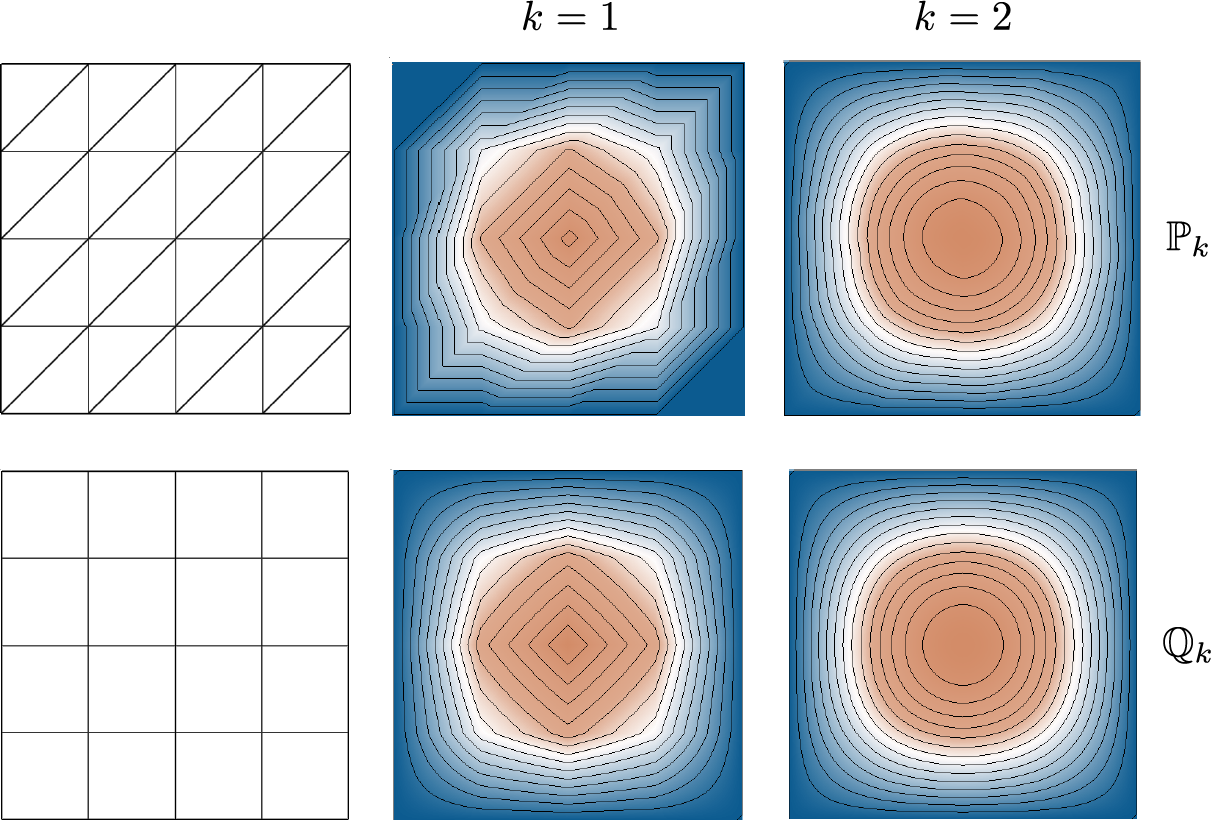
\includegraphics[scale=0.5]{images/comparaison_P_1_P_2.png}
    \caption{Solutions éléments finis de $-\triangle u=2\pi^2sin(\pi x)sin(\pi y)$ dans $\Omega$, $u=0$ sur $\partial\Omega$. Gauche: Maillage triangulaire et quadrilatéral. Milieu: Éléments d’ordre un. Droite: Éléments d’ordre deux. Source : \cite{reberol2018maillages}}.
    \label{fig:p1_vs_p2}
\end{figure}

Les éléments Qk se révèlent être un choix optimal pour aborder des problèmes exigeant une précision extrême, tels que les simulations de déformations, la modélisation géométrique avancée et l'interpolation de formes complexes. Cependant, leur pertinence s'étend bien au-delà de ces domaines, trouvant des applications étendues dans des champs comme la mécanique. Par exemple, des adaptations spécifiques sont souvent appliquées pour répondre aux besoins particuliers de certaines applications, telles que l'utilisation de quadratures réduites ou l'intégration de modes de déplacement incompatibles \cite{reberol2018maillages}.

Ce qui est remarquable du point de vue de la méthode des éléments finis, c'est que les quadrilatères et les hexaèdres se profilent comme des candidats plus intrigants dans certaines situations. Dans ces contextes, les éléments d'ordre 2 peuvent être astucieusement ajustés pour rivaliser avec la précision des tétraèdres quadratiques, mais avec l'avantage non négligeable d'une complexité de calcul notablement réduite. Cette caractéristique rend les quadrilatères et les hexaèdres particulièrement attrayants pour des simulations et des analyses pointues où l'efficacité computationnelle joue un rôle crucial.

Un autre avantage majeur des éléments Qk est leur utilisation plus efficace des nœuds dans le maillage. Contrairement aux éléments Pk, qui nécessitent davantage de nœuds pour représenter des polynômes de degré supérieur, les éléments Qk utilisent moins de degrés de liberté par élément, ce qui entraîne un maillage plus simple et des temps de calcul plus courts. Pour les simulations de grande échelle ou les problèmes nécessitant des ressources de calcul limitées, les éléments Qk sont donc une option attrayante.

\subsubsection{Maillage triangulaire vs maillage quadrilatéral}

Il est également intéressant de noter que les maillages quadrilatéraux ont besoin de moins d’éléments que les maillages triangulaires pour couvrir la même surface. Par exemple il faut au minimum deux triangles pour mailler un carré unité. De plus, il y'a moins d'arêtes dans un maillage quadrilatéral. Ces diférences se révèlent significatives pour des méthodes comme la méthode de Galerkin discontinue où il faut calculer des flux entre éléments, ou encore les méthodes d’hybridation. D'autres part, en élasticité linéaire et avec la formulation en déplacement, les triangles linéaires sont particulièrement connus pour leurs mauvaises performances, car le maillage ne se déforme pas autant qu'il devrait \cite{reberol2018maillages}.

\subsubsection{Etirement anisotropique}

L'étirement anisotropique permet de contrôler la déformation d'un maillage d'une manière plus ciblée. Dans certaines situations, il est nécessaire de préserver la forme dans certaines directions tout en autorisant des déformations plus importantes dans d'autres directions. Selon la théorie de l'approximation, pour une surface donnée et une allocation de points déterminée, la manière la plus optimale d'obtenir une approximation de qualité est d'utiliser un maillage où les éléments sont agencés de manière rapprochée le long des directions principales de courbure \cite{d2000bilinear}. Par exemple, dans la modélisation de tissus biologiques ou de matériaux déformables, un étirement anisotropique peut permettre de simuler avec précision les caractéristiques de déformation du matériau. En mécanique des fluides, particulièrement pour les fluides visqueux, il est très important de modéliser avec un maillage très raffiné le comportement du fluide au contact d’un obstacle, car des variations très fortes des champs ont lieu dans cette couche limite \cite{reberol2018maillages}. De même, il est souhaitable de comprimer les éléments dans la direction normale de l'aile d'un avion car les phénomènes physiques les plus significatifs se produisent dans la couche limite \cite{bommes2013quad}.

Du fait que la couche limite tend généralement à être localement plane, avec une concentration notable dans la direction perpendiculaire à la surface, l'utilisation de maillages structurés se révèle particulièrement appropriée pour son modélisme. Cette pertinence est renforcée par la caractéristique des hexaèdres qui peuvent présenter une grande anisotropie tout en préservant des angles droits. 

\subsubsection{Structure tensorielle}

 La structure tensorielle dans le contexte des éléments quadrilatéraux se réfère au fait que côtés ou les arêtes de ces éléments sont naturellement alignés avec les axes de coordonnées. Cela signifie que les directions tangentes et normales sont bien définies le long de ces côtés ou arêtes. Cette propriété intrinsèque simplifie la définition et l'interprétation des fonctions de base dans les cas où les comportements physiques ou mathématiques dépendent de ces directions.
 
 Lors de la modélisation des ondes électromagnétiques par exemple, il est essentiel de prendre en compte les propriétés de continuité et de compatibilité des composantes tangentielles et normales des champs. Les éléments quadrangulaires offrent une base solide pour satisfaire à ces exigences car leurs arêtes et faces partagées permettent un alignement naturel des composantes. En conséquence, il est généralement plus simple et plus efficace de définir des fonctions de base qui préservent les propriétés de continuité et de compatibilité sur ces types de maillages. Cela se traduit par une formulation discrète plus directe des équations de Maxwell, où les termes de sauts et de sauts normaux entre les éléments adjacents peuvent être calculés plus facilement. De plus, les interpolations des champs électromagnétiques aux nœuds du maillage sont plus cohérentes, ce qui peut conduire à des résultats numériques plus précis et stables.


Cependant, les maillages triangulaires peuvent être modifiés localement, ce qui leur permet de s’adapter plus facilement aux particularités des solutions.
Pour la mécanique, les quadrilatères/hexaèdres semblent plus intéressants, car ceux d'ordre 2 peuvent être modifiés afin d’atteindre des performances équivalentes aux tétraèdres quadratiques tout en conservant un coût de calcul bien inférieur.
Pour la propagation d’ondes électromagnétiques, l'optimisation des calculs numériques semble plus simple et efficace pour les éléments quadrilatéraux/hexaédriques qui ont naturellement une structure tensorielle.


%De plus, un certain nombre de modifications spécifiques à certaines applications (par ex. mécanique), comme l’utilisation de quadratures réduites ou de modes de déplacement incompatibles, sont couramment mises en oeuvre pour les quadrilatères et hexaèdres dans les logiciels commerciaux. Optimisation calculatoire de l’assemblage. Le calcul des coefficients (intégrales) repose sur des quadratures, c’est-à-dire des sommes pondérées. Lorsque les fonctions à intégrer sont des produits de polynômes uni-variés, comme c’est le cas pour Qk, il est possible de réduire le nombre d’opérations en factorisant des termes communs. Cette technique, dite de somme-factorisation, est particulièrement utile pour les polynômes d’ordres élevés et est une des raisons pour laquelle les maillages hexaédriques sont appréciés. Cette structure tensorielle rend également plus facile le développement de solveurs sans matrices, où les coefficients du système sont calculés à la volée lors de la résolution. Maillages structurés par blocs. Les maillages tétraédriques sont fondamentalement non structurés (par ex. valence des sommets très variable), il faut stocker toutes les informations de connectivité. Les maillages hexaédriques ont naturellement plus de régularité. Les maillages hexaédriques structurés sont combinatoirement équivalents à des grilles régulières. Dans ce cas, de nombreuses optimisations de calcul sont possibles, par exemple on peut connaitre à l’avance la largeur de bande des matrices creuses. Pour des géométries complexes, il n’est souvent pas possible d’utiliser des maillages globalement structurés, mais il est parfois possible de se ramener à des maillages structurés par blocs, pour lesquels ces optimisations peuvent être appliquées par bloc. Cette remarque ne s’applique pas à tous les maillages hexaédriques, mais la sous-catégorie des maillages structurés (par blocs) est très intéressante pour des applications hautes performances. Raffinement local. Comme les maillages hexaédriques sont plus ou moins structurés, il n’est généralement pas possible de leur appliquer des opérations de raffinement locales et de conserver un maillage conforme. Raffiner un hexaèdre engendre des modifications qui se propagent à travers une grande partie du modèle. Sur ce point, les maillages tétraédriques sont beaucoup plus flexibles, il existe d’ailleurs de nombreuses techniques de raffinement adaptatif pour ces derniers. Le raffinement adaptatif est particulièrement intéressant dans le cadre de la méthode des éléments finis puisqu’il 23 1.4. Variantes offre la possibilité d’augmenter la précision de la solution approchée tout en impactant peu le temps de calcul. Cette approche est parfois appelée h-FEM, car h caractérise la taille des éléments, en opposition à l’approche p-FEM où la précision de la solution est améliorée en augmentant le degré des polynômes d’interpolation. Les méthodes hp-FEM combinent ces deux outils. Nombre d’éléments et nombre de faces.  Maillages hex-dominants : generation, simulation et evaluation THESE presentee et soutenue publiquement le 23 mars 2018 pour l'obtention du Doctorat de l'Universite de Lorraine (mention informatique) par Maxence Reberol

 \subsubsection{Intégration numérique}

 Les méthodes de quadrature sont fréquemment utilisées dans le contexte de la simulation numérique pour calculer des quantités telles que l'aire d'un quadrilatère déformé, le moment d'inertie, ou d'autres intégrales associées à des propriétés physiques. Ces quantités nécessitent souvent l'intégration de fonctions sur les éléments (triangles, quadrilatères) déformés. Les méthodes de quadrature adaptées à la géométrie et à la structure tensorielle du quadrilatère permettent d'approximer ces intégrales de manière efficace et précise.
 
Lorsqu'on travaille avec des maillages triangulaires, les formules d'intégration numérique doivent prendre en compte les coordonnées barycentriques. Ces coordonnées sont utilisées pour représenter un point à l'intérieur d'un triangle en fonction de ses sommets. Cela peut rendre les formules d'intégration plus complexes à définir et à calculer. Les transformations entre les coordonnées réelles et barycentriques ainsi que les calculs associés peuvent ajouter une couche de complexité. En revanche, les maillages quadrangulaires ont des avantages en termes de simplicité. Puisque les éléments sont des quadrilatères, les coordonnées barycentriques ne sont pas nécessaires pour effectuer des calculs d'intégration. Les formules d'intégration sur des quadrilatères sont plus intuitives, car vous pouvez généralement utiliser des coordonnées cartésiennes standard pour décrire les points à l'intérieur de chaque élément. Cela simplifie grandement les calculs et les rend plus compréhensibles.

Les quadrilatères peuvent être plus facilement paramétrés en utilisant des coordonnées locales qui varient de 0 à 1 dans les deux directions principales. Cette paramétrisation facilite la définition des fonctions d'intégration et réduit la complexité des transformations géométriques et les calculs de jacobienne.\\


Toutefois, si la génération de maillages simplextiques (triangles) est très développée depuis plus d'un demi-siècle, celle de quadrilatères ou d'hexaèdres est plus problématique.
Dans le cas du maillage triangulaires, des algorithmes sont disponibles même pour des géométries très complexe. Cependant, les algorithmes de génération de maillage quadrilatéral automatisé sont disponibles pour une classe de géométries très limitée. Malgré les avancées dans la génération de maillages automatisés, la création de maillages de haute qualité reste un défi dans de nombreux cas, en particulier pour les géométries complexes. De ce fait, la génération de maillages demeure un domaine de recherche actif et important \cite{shepherd2008hexahedral}.

\section{Maillage}

Un maillage est une discrétisation d'un espace ou d'un domaine en cellules élémentaires (triangle ou rectangles en 2D, tétraèdres ou hexaèdres en 3D). De manière plus générale, un assemblage d’éléments, est considéré comme un maillage si \cite{george2013mesh}:\\

\begin{itemize}
\item l’union des éléments est une approximation de l’objet ou du domaine,\\
\item l’intérieur de chaque élément n’est pas vide,\\
\item l’intersection de l’intérieur de deux éléments est vide.\\
\end{itemize}

 Dans le contexte de la résolution des équations aux dérivées partielles en deux dimensions (2D), il existe différents types de maillages utilisés pour la discrétisation du domaine. Passons en revue quelques-uns de ces types de maillages couramment utilisés.

\subsection{Maillages à bases de triangles}


Il y a diverses approches pour créer des maillages en utilisant des triangles. On peut les regrouper en trois grandes catégories : les méthodes de type Delaunay, les méthodes basées sur des fronts et les méthodes de découpe spatiale, comme évoqué dans la référence \cite{botella2016generation}.

\subsubsection{Méthode de Delaunay}
Les méthodes de type Delauney se basent sur le critère de Delauney. Ce critère parfois appelé "propriété de la boule vide", stipule pour tout triangle, aucun sommet ne doit être contenu dans la boule ouverte correspondant au cercle circonscrit au triangle.

Bien que le critère de Delaunay soit connu depuis de nombreuses années, ce n'est que grâce aux travaux de Charles Lawson et Dave Watson que le critère a été largement popularisé et utilisé dans les méthodes de maillage \cite{owen1998survey}. La règle de Delaunay, en soi, ne constitue pas un algorithme pour générer des maillages. Elle représente plutôt un critère qui guide la manière de connecter un ensemble de points préexistants dans l'espace. Pour mettre en place un maillage, il est nécessaire de définir les emplacements des nœuds à l'intérieur de la géométrie. Une approche courante consiste d'abord à mailler la frontière de la géométrie, créant ainsi un ensemble initial de nœuds. Ensuite, les nœuds le long de cette frontière sont connectés pour former des triangles qui respectent la règle de Delaunay. À mesure que de nouveaux nœuds sont insérés itérativement dans le maillage existant, les triangles ou tétraèdres à une échelle locale sont ajustés pour maintenir en permanence la conformité à la règle de Delaunay. Ce qui distingue une méthode de génération de maillage de type Delaunay d'une autre, ce sont les algorithmes spécifiques utilisés pour déterminer les positions des nœuds à l'intérieur de la géométrie.\cite{owen1998survey}.

\paragraph{Maillage de Delauney-Voronoï}
Dans ce processus, on détermine la disposition géométriquement optimale d'un ensemble de sommets. Pour y parvenir, on réalise un échantillonnage du modèle en plaçant les points de manière aléatoire ou en suivant une heuristique spécifique. Ensuite, la position géométrique de ces points est affinée en minimisant une fonction objectif qui reflète une distribution idéale prédéfinie \cite{botella2016generation}. Ensuite, les diagrammes de Voronoï de ces points sont générés :

\begin{definition}[\cite{hecht2007maillage}, voir figure \ref{fig:voronoi_diagram}]
Soit un ensemble de points $\mathcal{S}=\{x^i\in\mathbb{R}^2, i\in\llbracket 1, N_p\rrbracket\}$. Les diagrammes de Voronoï sont les polygones convexes $V^i$, pour $i\in\llbracket 1, N_p\rrbracket$, formés par l’ensemble des points de $\mathbb{R}^2$ qui sont plus proches de $x^i$ que des autres points $x^j$. Formellement, on a:
\begin{eqnarray}
V^i=\{x\in\mathbb{R}^2\ |\ |x-x^i|\leq|x-x^j|,\ \forall j\in\llbracket 1, N_p\rrbracket\}.
\end{eqnarray}
\end{definition}

\begin{figure}[!h]
    \centering
    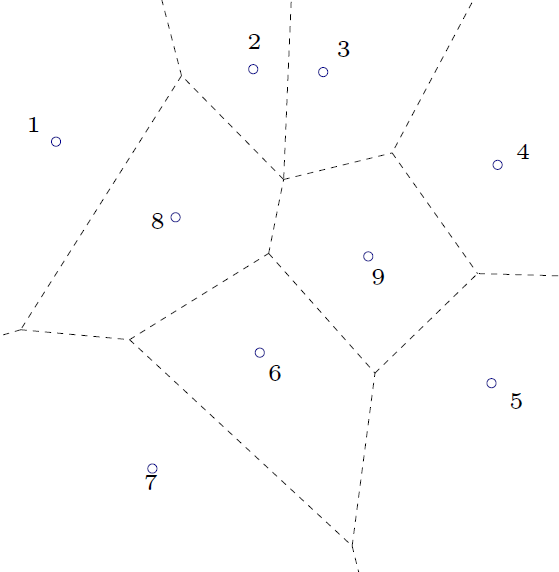
\includegraphics[scale=0.55]{images/voronoi_diagram.png}
    \caption{Diagramme de Voronoï. Source : \cite{hecht2007maillage}.}
    \label{fig:voronoi_diagram}
\end{figure}

Le maillage de Delaunay est ensuite généré en tant que maillage dual des diagrammes de Voronoï. Deux points $x_i$ et $x_j$ sont reliés dans ce maillage si les diagrammes de Voronoï $V_i$ et $V_j$ partagent un segment en commun (voir figure \ref{fig:maillage_delauney}). Afin d'obtenir un maillage triangulaire, il suffit de diviser les polygones qui ne sont pas déjà des triangles en triangles.

\begin{figure}[!h]
    \centering
    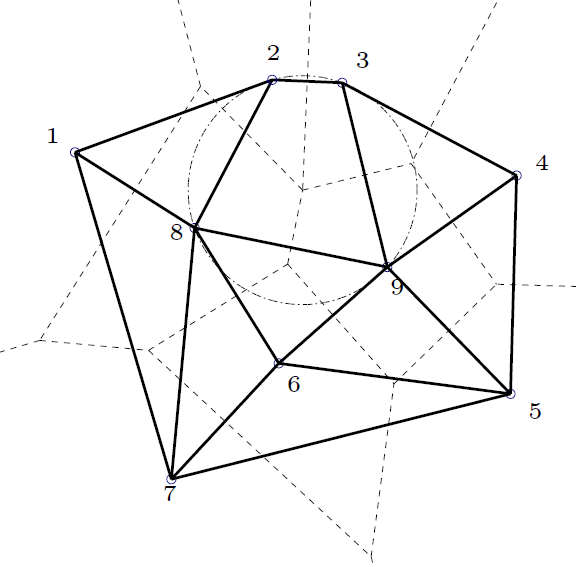
\includegraphics[scale=0.55]{images/Maillage_delauney.png}
    \caption{Maillage de Delauney. Source : \cite{hecht2007maillage}.}
    \label{fig:maillage_delauney}
\end{figure}

\paragraph{L'algorithme de Bowyer-Watson} construit les triangulations de Delaunay par induction \cite{bowyer1981computing, watson1981computing, ern2004theory}.
 est une méthode de triangulation de Delaunay en 2D. Son objectif est de générer un maillage de triangles de Delaunay pour un ensemble de points donné dans le plan. L'algorithme commence par créer un triangle géant qui englobe tous les points de l'ensemble. Ensuite, il ajoute chaque point un par un dans le maillage en respectant la règle de Delaunay, c'est-à-dire que le cercle circonscrit de chaque triangle du maillage doit être vide, ne contenant aucun autre point de l'ensemble. Pour ajouter un point dans le maillage, l'algorithme identifie tous les triangles du maillage qui sont affectés par l'ajout du nouveau point. Il supprime ces triangles du maillage et forme de nouveaux triangles avec le point ajouté comme sommet. Le processus se répète jusqu'à ce que tous les points soient ajoutés et que le maillage respecte la propriété de Delaunay.

Les méthodes de type Delaunay ne fournissent pas de garantie pour préserver la discrétisation des frontières du modèle. Deux stratégies sont mises en œuvre pour assurer que la discrétisation des limites soit préservée dans la triangulation de Delaunay \cite{botella2016generation}:\\

\begin{itemize}
    \item L'ajout de sommets le long des frontières jusqu'à ce qu'elles correspondent géométriquement. Cependant, cela peut altérer la discrétisation initiale \cite{cohen2002conforming}.\\
    \item Effectuer des modifications locales sur le maillage pour obtenir la discrétisation initiale des frontières. Une description détaillée de ce processus est donnée dans les ouvrages de George et Borouchaki \cite{george1997triangulation} ainsi que de Hecht \cite{hecht2007maillage}.
    
    Considérons que l'arête $(\alpha, \beta)$ ne fait pas partie du maillage de Delaunay. Nous analysons les diagonales $(a, c)$ des quadrilatères $(a, b, c, d)$ convexes constitués de deux triangles $(a, b, c)$ et $(b, c, d)$ où la diagonale $(a, c)$ coupe $(\alpha, \beta)$. Si l'arête $(b, d)$ ne coupe pas $(\alpha, \beta)$, nous procédons à l'échange de diagonales. Dans le cas contraire, l'échange de diagonales est effectué de manière aléatoire. Du fait qu'il existe une solution au problème, le recours aux échanges de diagonales de manière aléatoire permet de converger, car, statistiquement, tous les maillages possibles sont parcourus et ils sont en nombre fini.
\end{itemize}


\subsubsection{Méthode frontale}

La méthode d'avancée de front \cite{george1994advancing, lohner1996progress, lohner2014recent} se distingue par son approche qui débute avec une frontière préalablement définie constituée d'un ensemble d'arêtes qui reste inchangée tout au long du processus de génération du maillage. Cette frontière triangulée est considérée comme le front à partir duquel de nouveaux éléments sont progressivement ajoutés.

À chaque itération, il est décidé où positionner le prochain sommet du front. Cette décision est généralement prise en recherchant la position la plus appropriée sur la frontière, dans le but de réduire les déformations des triangles et d'assurer une qualité élevée du maillage. Cependant, dans certaines situations particulières, on peut préférer d'autres critères en fonction des besoins spécifiques de l'application. Par exemple :\\

\begin{itemize}
    \item Critère de Delaunay : le sommet est sélectionné de manière à respecter le critère de Delaunay, ce qui implique que le cercle circonscrit au nouveau triangle formé ne doit pas englober d'autres points de la géométrie.\\
    \item Critère de qualité de l'élément: pour garantir que tous les triangles du maillage ont des angles proches de 60 degrés ou satisfont d'autres propriétés de forme souhaitées\\
    \item Critère de densité: pour contrôler la taille des éléments dans différentes régions du domaine. Par exemple, on peut souhaiter avoir des éléments plus petits dans les régions où des variations importantes du champ numérique sont attendues\\
\end{itemize}


Les bords des triangles initiaux du front deviennent alors des faces intérieures du maillage, tandis qu'un nouveau jeu de faces de front est créé. Ce cycle continue jusqu'à ce que le maillage couvre entièrement le domaine. Ainsi, cette approche assure une discrétisation cohérente du domaine en suivant rigoureusement la frontière prescrite, et ce, de manière incrémentale \cite{baker2005mesh}.

Au fur et à mesure de l'avancement du front, il devient possible d'enrichir la qualité du maillage en procédant à des opérations de raffinement. Ces opérations englobent l'insertion de points au milieu des arêtes ainsi que l'ajustement des positions des sommets, permettant ainsi une meilleure adaptation aux courbes présentes sur la surface. Il est également envisageable de prendre en considération d'autres contraintes particulières, telles que les conditions aux limites, ou encore des critères spécifiques de qualité de maillage au sein de zones spécifiques de l'objet.

Une difficulté particulière avec cette méthode survient dans les étapes finales lorsque le front se réduit progressivement et les derniers espaces vides sont remplis par de nouveaux éléments. Cela est illustré sur la figure \ref{fig:moving_front_method}, où l'on peut voir une triangulation presque achevée de la région autour d'un profil d'aile, avec les arêtes du front actuel marquées en gras.  Une étape d'optimisation peut alors être requis pour une disposition optimale des sommets \cite{botella2016generation}.

\begin{figure}[!h]
    \centering
    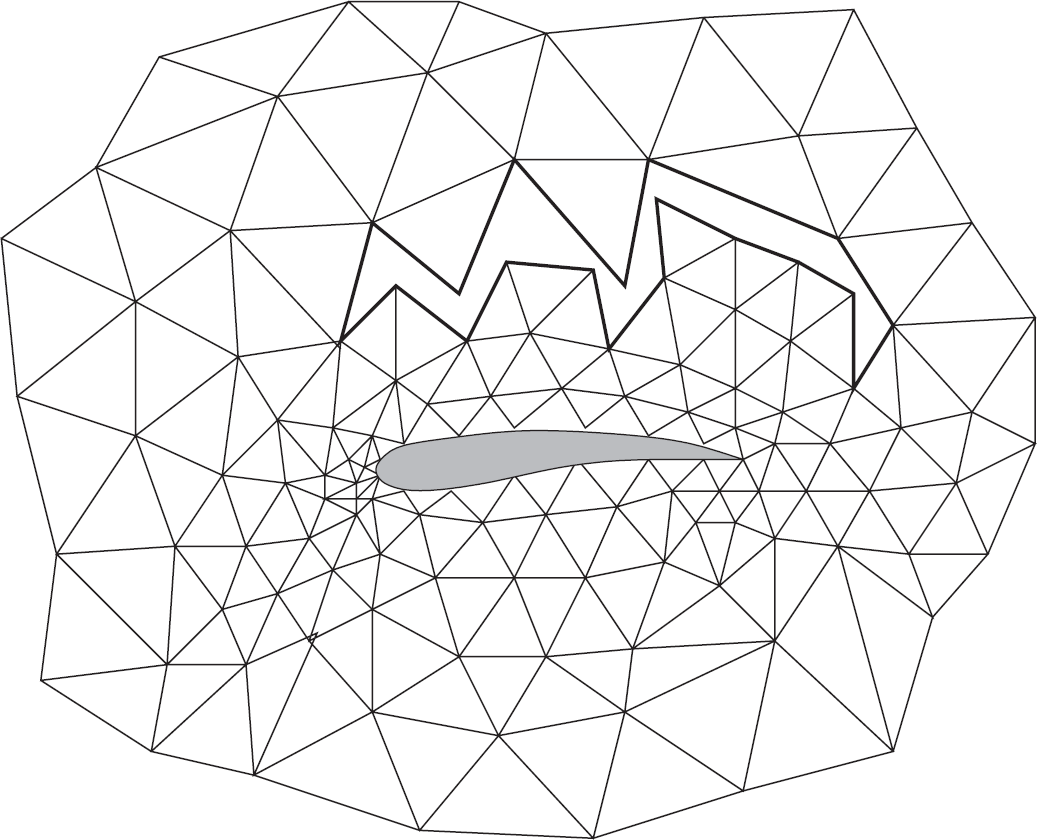
\includegraphics[scale=0.35]{images/moving front method.png}
    \caption{Phase de fermeture de la méthode du frontale. Source : \cite{baker2005mesh}.}
    \label{fig:moving_front_method}
\end{figure}


La méthode d'avancée de front est relativement aisée à implémenter et peut être efficace pour des géométries simples ou modérément complexes. Cependant, pour des géométries très complexes ou avec des trous, il peut être difficile de construire une frontière active appropriée, et le maillage résultant peut contenir des triangles de mauvaise qualité.

Il existe différentes variantes de la méthode d'avancée de front qui peuvent être adaptées en fonction des caractéristiques de la géométrie à mailler et des exigences du problème. Des améliorations peuvent être apportées pour contrôler la qualité des triangles, optimiser la distribution des points, gérer les singularités ou les contours concaves, etc. En général, la méthode d'avancée de front est un outil polyvalent et largement utilisé pour la génération de maillages triangulaires dans de nombreuses applications scientifiques et d'ingénierie.

\subsubsection{Méthode de décomposition spatiale (Quadtree)}

Introduite par  \cite{yerry1983finite}, cette procédure peut être vue comme une division du domaine en une collection de rectangles, suivie d'une division de ces rectangles en triangles \cite{baker2005mesh}.

Ces méthodes se basent sur une structure d'arbre qui est une représentation hiérarchique des différentes subdivisions de l'espace. Schématiquement, l'approche de maillage basée sur les quadtrees se compose des étapes suivantes:

%de trois étapes successives et peut être résumée comme suit  Un premier rectangle est formé, qui contient tous les points du contour. La méthode consiste à découper, à partir de ce rectangle initial, chaque rectangle en 4 rectangle, de façon récursive, tant que les limites du modèle intersectent la cellule, jusqu’à un critère d’arrêt . Ce critère d’arrêt peut être conditionné par la taille d’éléments locale souhaitée, par la courbure du modèle présent dans la cellule, ou un nombre de subdivisions. Un autre critère, permettant de conserver la topologie du modèle, est de minimiser le nombre de composantes connexes de l’intersection entre le modèle et une cellule \cite{botella2016generation}. Schématiquement, l'approche de maillage basée sur les quadtrees se compose de trois étapes successives et peut être résumée comme suit \cite{pascal1998fast}:\\

\begin{enumerate}
    \item Initialisation : on commence par définir le domaine global à mailler puis on crée un quadrilatère initial qui le représente.
    
    \item Subdivision du quadtree : le quadrilatère initial est divisé en quatre sous-quadrants de taille égale en traçant deux lignes verticales et deux lignes horizontales pour former une grille.
    
    \item Évaluation des critères : pour chaque sous-quadrant nouvellement créé, on évalue des critères de qualité de maillage tels que la taille des angles, la longueur des arêtes et d'autres mesures géométriques pour déterminer s'il est nécessaire de subdiviser davantage ou si le sous-quadrant est adéquat pour la triangulation.
    
    \item Triangulation des sous-quadrants : les sous-quadrants jugés appropriés pour la triangulation sont convertis en triangles en reliant leurs coins.
    
    \item Raffinement : si nécessaire, on effectue des opérations de raffinement, telles que l'ajout de points au milieu des arêtes ou l'ajustement des sommets pour mieux s'adapter aux caractéristiques de la surface.
    
    \item Itérations : répétez les étapes 3 à 5 pour les sous-quadrants nouvellement créés, en continuant à subdiviser et à trianguler jusqu'à ce que les critères de qualité de maillage soient satisfaits dans toutes les zones du maillage.
    
    \item Terminaison : on arrête le processus de subdivision et de triangulation lorsque les critères de qualité de maillage sont globalement atteints ou lorsque d'autres conditions de terminaison spécifiques sont satisfaites.
    
    \item Fin : le processus se termine avec un maillage triangulaire satisfaisant les critères de qualité établis pour la région donnée.
\end{enumerate}

Afin de ne pas avoir de trop grandes variations de taille d’éléments dans le maillage, la différence de niveaux de subdivision entre deux cellules adjacentes est limitée. Une fois la décomposition terminée, les sommets du maillage sont les coins des cellules de subdivisions et éventuellement les intersections entre les limites du modèle et les cellules. Les éléments du maillage sont alors construits en découpant les cellules \cite{botella2016generation}.


\begin{figure}[!h]
    \centering
    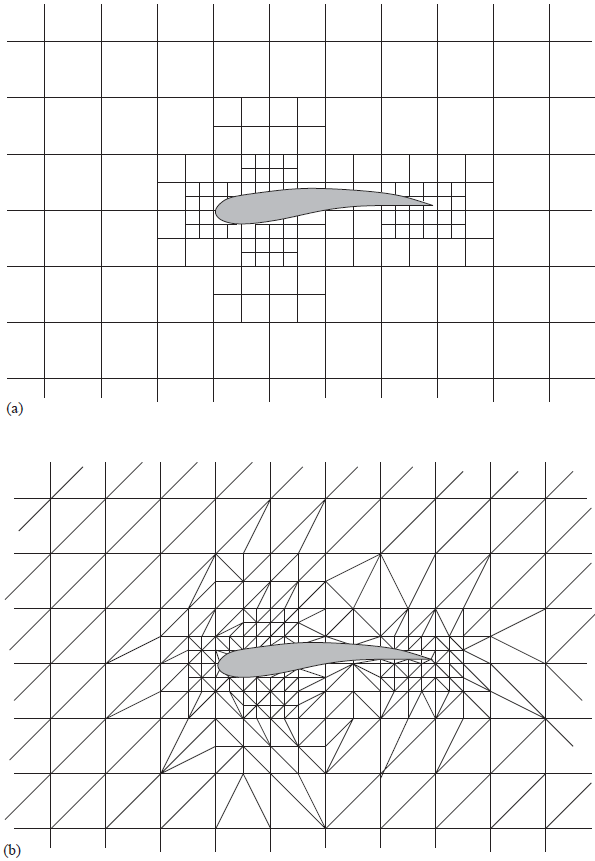
\includegraphics[scale=0.6]{images/octree decomposition.png}
    \caption{(a) Décomposition en octree de la région autour d'un profil aérodynamique. (b) Conversion de la décomposition en octree en une triangulation. Source : \cite{baker2005mesh}}
    \label{fig:octree decomposition}
\end{figure}

La méthode Quadtree permet de concentrer les ressources de maillage dans les zones les plus complexes ou les plus intéressantes, tout en conservant des éléments de maillage plus simples dans les régions homogènes. Cela conduit à une utilisation efficace des ressources de calcul et de stockage. Elle permet d'obtenir des maillages de haute résolution là où c'est nécessaire, tout en réduisant la complexité dans les zones moins critiques. Par ailleurs, elle gère efficacement les discontinuités géométriques et topologiques en adaptant la taille et la forme des éléments de maillage autour de ces régions, ce qui améliore la précision des simulations.

Cependant, la mise en œuvre de cette méthode nécessite des algorithmes sophistiqués pour gérer la subdivision récursive, la fusion de carrés et la gestion des bordures. Le choix des critères pour la subdivision et le raffinement des carrés peut être complexe et dépendant de l'application, ce qui nécessite une expertise dans le domaine concerné. Pour finir, l'adaptation du maillage près des frontières du domaine peut nécessiter une attention particulière pour éviter des problèmes de cohérence.

%Compte tenu de leur régularité, les maillages structurés sont géométriquement peu flexibles et le plus souvent constitués de quadrilatères. Ces maillages sont fréquemment appelés des grilles. En revanche, les maillages non structurés peuvent être composés de polygones quelconques, ce qui augmente leur capacité à représenter des géométries complexes. Si le maillage est composé de plusieurs types d’éléments différents, il est dit multi-éléments ou mixte \cite{ref7}.\\
%Lors des simulations numériques, le maillage se révèle indispensable puisqu'il est le support de méthodes numériques telles que les éléments finis, les volumes finis ou les différences finies. Il joue non seulement le rôle de partition du domaine, mais aussi de support pour les polynômes d'interpolation utilisés. Il permet notamment de générer des systèmes linéaires creux que l’on peut résoudre efficacement.\\
%Les simulations numériques requièrent donc la construction de "bons maillages". Ils doivent représenter suffisamment les géométries présentes dans la scène de calculs en fonction des physiques étudiées et posséder des éléments de "bonnes qualités" afin d'assurer de bonnes propriétés aux schémas numériques (précision, conditionnement du système linéaire). Ci-dessous, nous présentons quelques méthodes de construction de maillages.

\subsection{Maillages à bases de quadrilatères}

Les maillages à bases de quadrilatères sont caractérisé par la nature des sommets qui les composent. Un sommet dans un tel maillage est dit \emph{régulier} si sa \emph{valence} topologique est égale à 4; sinon il est dit \emph{irrégulier}. La valence topologique d'un sommet est le nombre de faces adjacentes à ce sommet. Avec cette propriété, les maillages quadrilatéraux peuvent être décrit en terme de régularité de la manière suivante \cite{bommes2013quad} (voir figure \ref{fig:Quad_meshes_categories}):\\

 \begin{itemize}
    \item Maillage non-structuré : une grande partie des sommets du maillages sont des sommets irréguliers,\\
    \item Maillage à valence semi-régulière : la plupart des sommets du maillage sont des sommets réguliers,\\
    \item Maillage semi-régulière : il s'agit d'un maillage formé de plusieurs partitions. Chaque partition est un réseau de quadrilatères de sommets réguliers, et l'ensemble est assemblé de manière \emph{conforme}, c'est-à-dire que les interfaces entre les partitions s'ajustent de manière cohérente,\\
    \item Maillage régulier :  il ne contient aucun sommet irrégulier. Un maillage régulier est topologiquement équivalent à une grille régulière.\\
 \end{itemize}
 
\begin{figure}[!h]
    \centering
    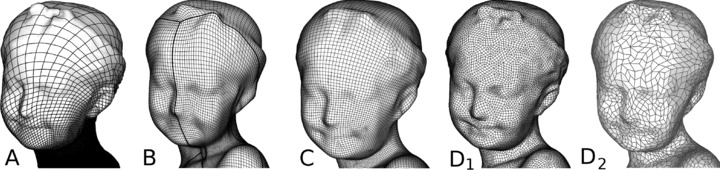
\includegraphics[scale=5.2]{images/Quad_meshes_categories.png}
    \caption{Catégories de maillage quadrilatéral. A: régulier; B: semi-régulier; C: valence semi-régulier; D1-D2: non-structuré (D2 plus irrégulier que D1). Source: \cite{bommes2013quad}.}
    \label{fig:Quad_meshes_categories}
\end{figure}


Dans le contexte des simulations numériques, les caractéristiques recherchées pour les maillages quadrilatéraux revêtent une importance significative. Les attributs visés se déclinent généralement comme suit :\\

\begin{itemize}
    \item Minimalité des irrégularités : il est préférable d'avoir le moins possible de points irréguliers dans les maillages. La minimisation de ces irrégularités contribue à maintenir la cohérence et la régularité du maillage, améliorant ainsi la stabilité et la précision des simulations.\\
    \item Alignement le long de la frontière : il est souhaitable que les éléments du maillage soient alignés le long des bords du domaine permettant ainsi de donné une description fidèle du bord du domaine.\\
    \item Éléments de haute qualité : il est recommandé d'utiliser des éléments dont les contours se rapprochent au maximum de la configuration d'un carré ou d'un rectangle. En utilisant un maillage composé d'éléments qui présentent des formes régulières, on peut minimiser les risques de dégénérescence lors des transformations géométriques causées par des éléments déformés ou excessivement étirés.\\
    \item Respect des contraintes de taille : il est essentiel que les éléments du maillage satisfaissent aux exigences de taille définies. Cette condition garantit que le maillage capture de manière appropriée les variations locales de la solution, en allouant davantage de détails là où c'est nécessaire, tout en maintenant une efficacité numérique globale.\\
    \item Insensible à l'orientation. La rotation ou la translation d'une géométrie donnée ne devrait pas changer la topologie du maillage résultant. Un maillage généré dans une géométrie transformée devrait être équivalent au maillage original transformé.\\
\end{itemize}

Générer des maillages qui incorporent simultanément chacune de ces propriétés constitue un défi ardu. Très souvent, la poursuite de l'une de ces caractéristiques entre en conflit avec la quête d'optimisation d'une autre. Plusieurs approches ont été développées pour la génération de maillages quadriatères. Ces approches varient en fonction des besoins spécifiques des applications, de la complexité de la géométrie à mailler et des contraintes de qualité du maillage requis. 

\subsubsection{Décomposition de maillages triangulaires en quadrangles}

Les méthodes de conversion de maillages triangulaires en maillages quadrangulaires, également appelées \emph{méthodes de maillage tri-to-quad}, visent à transformer des maillages constitués de triangles en maillages contenant principalement des quadrilatères (quads).  Il existe plusieurs approches pour effectuer cette conversion, chacune ayant ses avantages et ses limitations. Voici quelques-unes des méthodes couramment utilisées :

Sous-division de Catmull-Clark: Une approche naïve pour convertir n'importe quel maillage polygonal en un maillage quadrangulaire consiste à appliquer la subdivision topologique de Catmull-Clark \cite{catmull1998recursively} en divisant tous les triangles en trois quadrangles (voir figure \ref{fig:tri_to_quad_1}). Le maillage quadrangulaire ainsi obtenu conserve toutes les arêtes d'origine, mais présente également plusieurs inconvénients majeurs : il augmente le nombre d'éléments et introduit de nombreux sommets irréguliers. Cette option est praticable uniquement si le maillage de départ est déjà principalement constitué de quadrangles et qu'une augmentation de la complexité est acceptable. Dans la plupart des cas, des approches plus élaborées s'avèrent nécessaires \cite{bommes2013quad}.

\begin{figure}[!h]
    \centering
    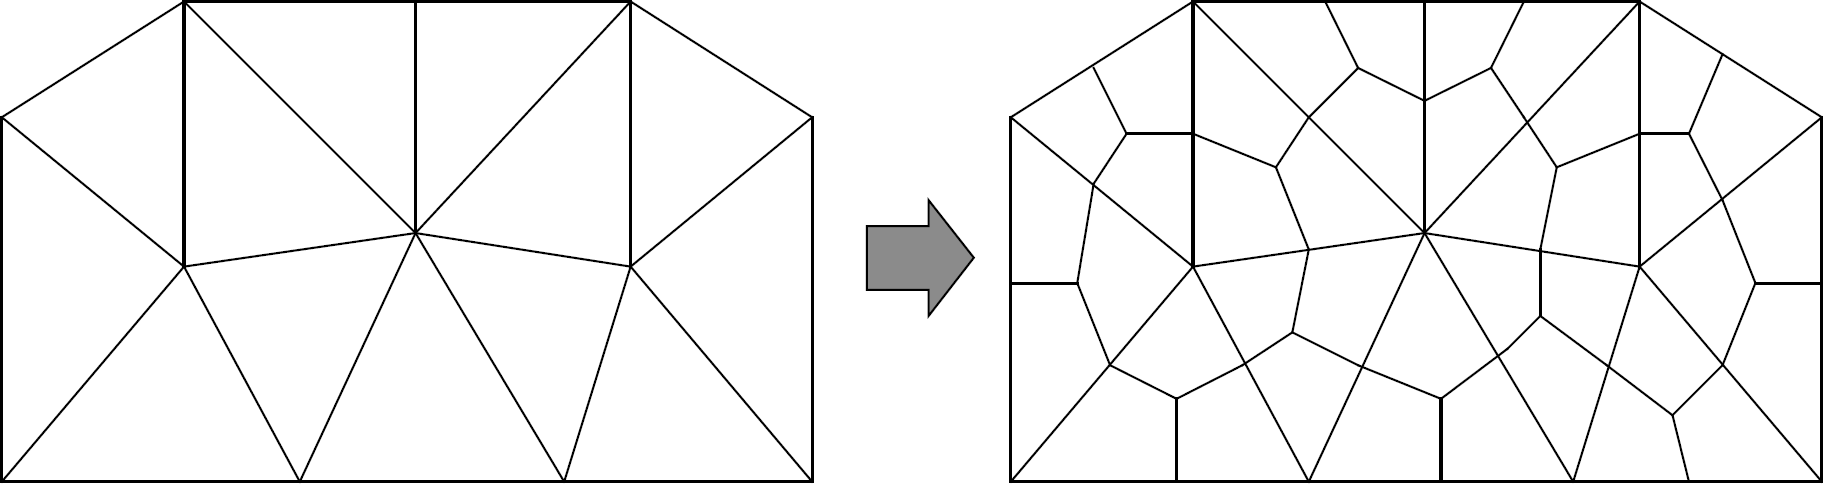
\includegraphics[scale=0.42]{images/tri_to_quad_1.png}
    \caption{Génération de maillage quadrilatéral par subdivision de chaque triangle en quatre quadrangles. Source : \cite{owen1998survey}.}
    \label{fig:tri_to_quad_1}
\end{figure}

Combinaison de triangles: il s'agit de convertir un maillage triangulaire en maillage quadrangulaire via des opérations sur la connectivité. Le mécanisme principal consiste à fusionner deux triangles originaux en un quadrilatère ; en substance, la conversion de maillage triangulaire en maillage quadrangulaire repose sur la mise en paire des triangles adjacents d'origine \cite{bommes2013quad} (voir figure \ref{fig:tri_to_quad_2}). La méthode de combinaison de triangles peut être améliorée si l'on fait attention à l'ordre dans lequel les triangles sont combinés \cite{owen1998survey}. L'algorithme définit dans \cite{lo1989generating} propose plusieurs procédures heuristiques pour l'ordre dans lequel les triangles pourraient être combinés. Il en résulte un maillage à dominante de quadrilatères contenant un nombre minimal de triangles. Dans \cite{owen1998quad}, les auteurs utilisent une approche d'avancée de front pour convertir les triangles en quadrilatères, mais parvient à réduire considérablement le nombre de noeuds irréguliers dans le maillage. Des échanges locaux d'arêtes sont effectués et des nœuds supplémentaires sont introduits afin d'assurer l'alignement avec la frontière et l'orthogonalité. Un nombre quelconque de triangles peut être supprimé pour créer un seul quadrilatère.

\begin{figure}[!h]
    \centering
    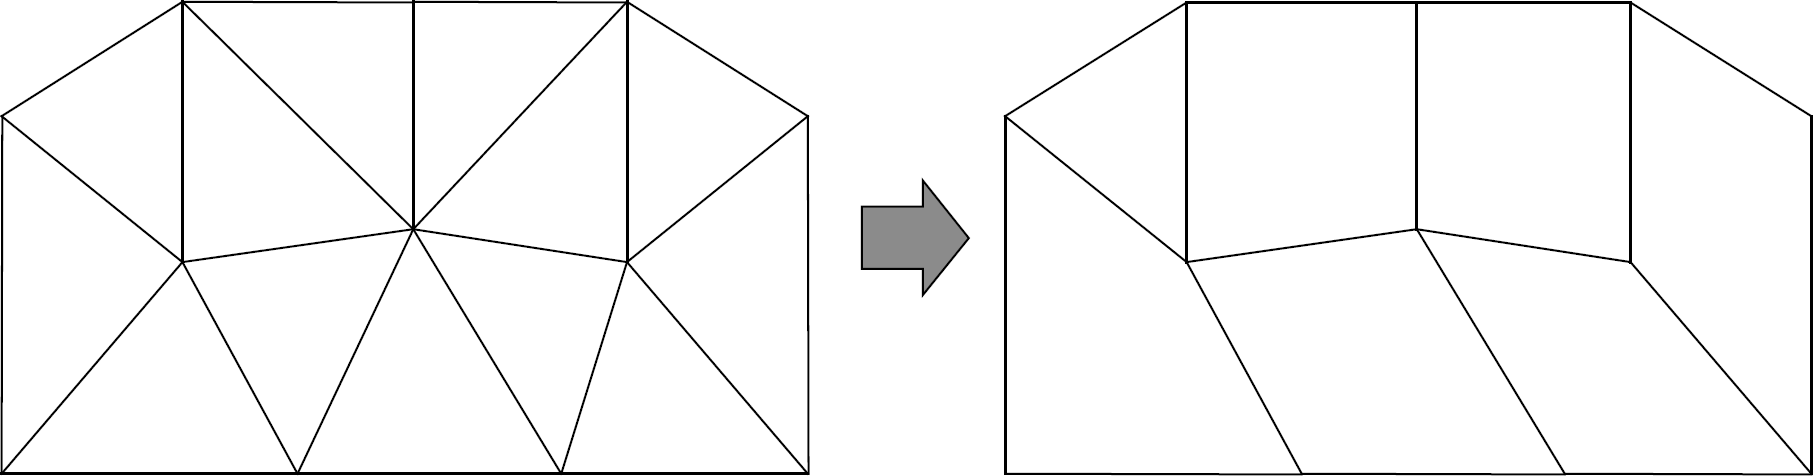
\includegraphics[scale=0.42]{images/tri_to_quad_2.png}
    \caption{Combinaison de triangles. Source : \cite{owen1998survey}.}
    \label{fig:tri_to_quad_2}
\end{figure}

D'autres algorithmes sont présenté dans \cite{bommes2013quad} tel que le SQuad \cite{gurung2011squad} conçu pour améliorer la représentation interne des maillages, mais  qui peut être utilisé pour définir un maillage quadrangulaire à partir d'un maillage triangulaire ou encore BlossomQuad \cite{remacle2012blossom} qui exploite un algorithme d'appariement parfait issu de l'optimisation combinatoire. Cependant, sa complexité algorithmique est quadratique par rapport au nombre d'éléments. Cela rend la méthode chronophage et principalement adaptée aux cas où l'optimalité du résultat est plus importante que le temps d'exécution.

\subsubsection{Méthodes basées sur la paramétrisation}

Les méthodes de paramétrisation sont des techniques utilisées en infographie et en géométrie numérique pour générer des mappages paramétrés d'une surface donnée sur un domaine plus simple, souvent un carré ou un rectangle, qui peut ensuite être utilisé pour générer des maillages quadrilatéraux. Ce processus est couramment utilisé dans la génération de maillages à diverses fins, notamment la modélisation 3D, la simulation et le rendu. Voici quelques méthodes de paramétrisation courantes pour générer des maillages quadrilatéraux:

\paragraph{Paramétrisation plane:} Il s'agit de la forme la plus simple de paramétrisation où la surface est projetée sur un domaine plan, tel qu'un carré ou un rectangle. Cela implique d'attribuer des coordonnées de texture 2D aux sommets du maillage. Cette méthode convient aux surfaces qui peuvent être approximativement aplaties sans distorsion significative.

\paragraph{Paramétrisation harmonique:} La paramétrisation harmonique vise à réduire la déformation entre une surface et le domaine paramétrique. Pour y parvenir, on résout une équation de Laplace sur la surface en imposant des conditions aux limites spécifiques basées sur le domaine paramétrique cible. Cette méthode est particulièrement efficace pour les surfaces de genre zéro (surfaces sans anses ni trous) et peut produire des paramétrisations de haute qualité. Elle a pour effet de préserver les détails de forme locaux, ce qui en fait un outil prisé dans les domaines de l'architecture et de l'ingénierie. Le processus implique les étapes suivantes :\\

\begin{enumerate}
    \item Sélection de points d'ancrage sur la surface, correspondant à des sommets dans le domaine paramétrique.\\
    \item Attribution de valeurs paramétriques fixes à ces points d'ancrage.\\
    \item Résolution de l'équation de Laplace pour le reste de la surface, de manière à obtenir une cartographie fluide qui minimise la déformation.
\end{enumerate}



\subsubsection{Superposition de grille régulière}

Ces méthodes débutent par la création d'un maillage dont la génération dans une étendue convenable autour de l'objet peut varier en complexité. L'algorithme introduit par Schneiders \cite{schneiders1996grid} (voir figure \ref{fig:superpo_grid_1}) déploie une grille structurée pour recouvrir une zone considérable autour de l'objet. La taille de chaque cellule dans cette grille peut être déterminée de manière arbitraire. Il ne reste plus qu'à ajuster la grille à la frontière de l'objet. Pour se faire, les éléments extérieurs à l'objet ou trop proches de sa frontière sont éliminés du maillage initial, laissant les cellules restantes pour former la structure de base du maillage. Ensuite, la zone entre la frontière de l'objet et le maillage initial est comblée en utilisant la technique d'isomorphisme. Cette technique implique que chaque nœud sur la frontière du maillage initial est associé à un nœud correspondant sur la frontière de l'objet, ce qui permet de remplir la région avec des éléments quadrilatéraux.

 \begin{figure}[!h]
    \centering
    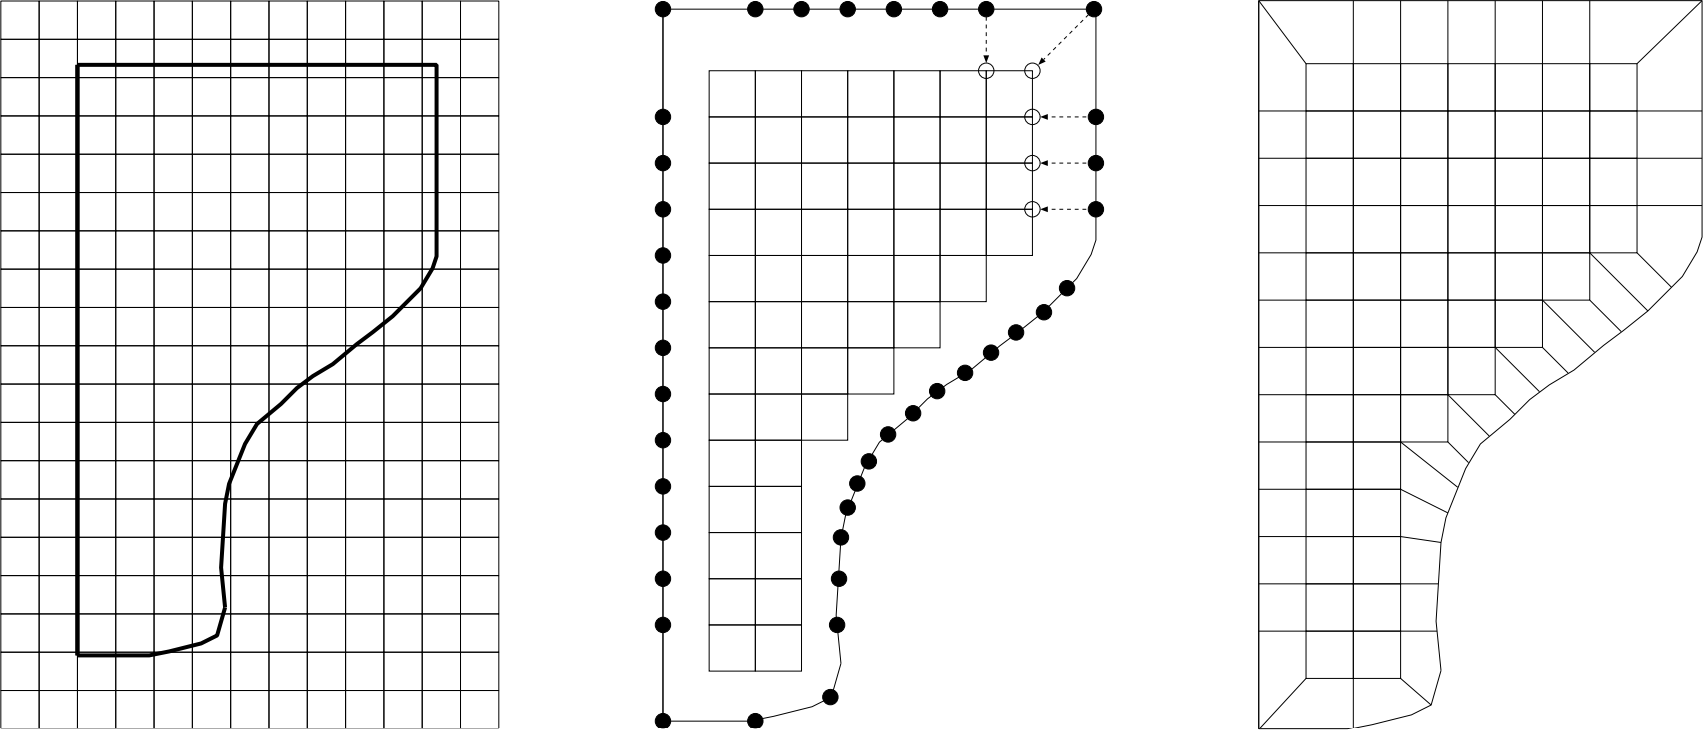
\includegraphics[scale=0.4]{images/superpo_grid_1.png}
    \caption{Méthode de superposition d'une grille régulière. Source : \cite{schneiders1996grid}.}
    \label{fig:superpo_grid_1}
\end{figure}

Dans \cite{taghavi1994automatic, ives1995geometric} les auteurs adoptent une autre méthode appelé méthode de projection  (voir figure \ref{fig:superpo_grid_2}). La grille initiale reste en place et les noeuds du maillage sont déplacés vers les arêtes de l'objet, de sorte que la frontière de l'objet soit entièrement recouverte par les arêtes du maillage. Le maillage est ensuite optimisé par un lissage laplacien.

 \begin{figure}[!h]
    \centering
    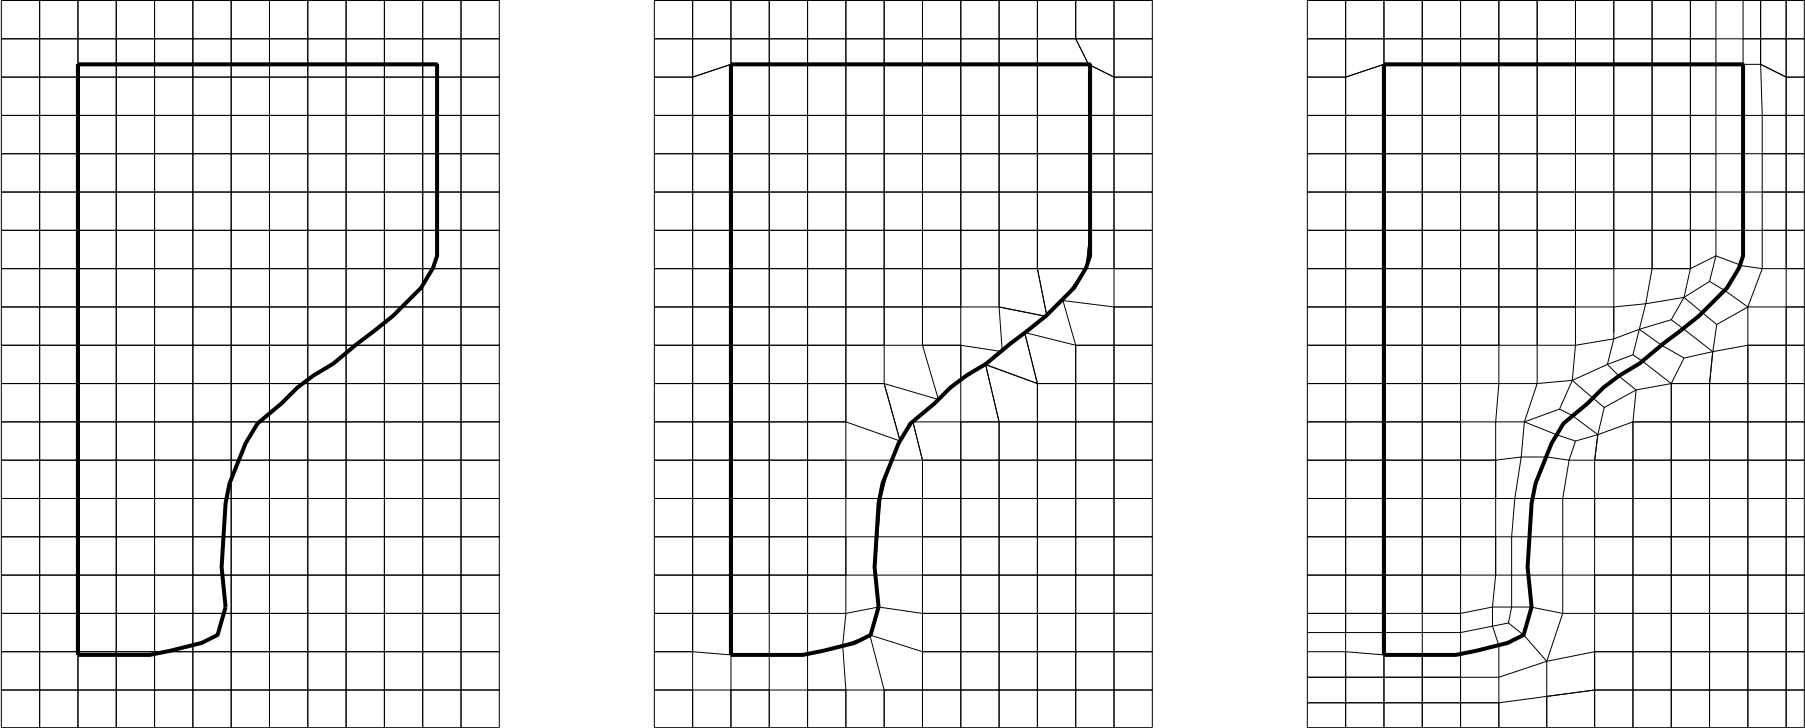
\includegraphics[scale=0.4]{images/superpo_grid_2.png}
    \caption{Méthode de projection. Source : \cite{schneiders1996grid}.}
    \label{fig:superpo_grid_2}
\end{figure}

\subsubsection{Méthode de l'axe médian}

La méthode de l'axe médian, également connue sous le nom de méthode de squelettisation, est une technique utilisée en infographie et en géométrie numérique pour générer des maillages quadrilatéraux à partir de formes complexes. Cette méthode vise à trouver une représentation simplifiée de la forme d'entrée en identifiant le "squelette" central ou l'"axe médian" de la forme. Cette méthode a d'abord été conçue par Nackman et Srinivasan \cite{nackman1989method}. Ils ont remarqué que l'axe médian présentait une décomposition naturelle bien définie de la surface et l'ont utilisé sans modifications pour diviser la surface en blocs. Quelques règles supplémentaires pour fusionner les blocs produits ont été élaborées pour améliorer l'adéquation de la décomposition. Une méthode améliorée a été proposée par Tam et Armstrong \cite{tam19912d} qui produit des décompositions de meilleure qualité.

Voici un aperçu de la manière dont fonctionne la méthode de l'axe médian pour la génération de maillages quadrilatéraux :\\

\begin{itemize}
    \item  Géométrie d'entrée : on commence avec une forme polygonale complexe et irrégulier. Cette forme peut représenter la limite d'un objet en 2D ou la surface d'un objet en 3D.\\

    \item Diagramme de Voronoi : la première étape consiste à calculer le diagramme de Voronoi de la forme d'entrée. Le diagramme de Voronoi divise l'espace autour de chaque point (ou sommet) de la forme en régions. Chaque région contient tous les points qui sont plus proches d'un sommet particulier que de tout autre sommet de la forme. Ces régions sont appelées cellules de Voronoi.\\

    \item Squelettisation (voir Figure \ref{fig:median_axis}): l'axe médian est essentiellement le dual du diagramme de Voronoi. Pour obtenir l'axe médian, on trouve les centres des cercles circonscrits pour chaque cellule de Voronoi. L'axe médian représente le "squelette" central de la forme d'entrée, qui capture ses principales caractéristiques et sa connectivité.\\

    \item Suppression des arêtes : dans l'axe médian, il y a souvent de nombreuses branches et arêtes qui ne sont pas pertinentes pour le maillage quadrilatéral souhaité. Ces branches superflues doivent parfois être supprimées ou élaguées pour simplifier le squelette tout en préservant les caractéristiques essentielles de la forme.\\

    \item Génération du maillage quadrilatéral : une fois que vous avez l'axe médian a été simplifié, on génère des éléments quadrilatéraux en connectant des paires de points proches sur le squelette. Ces connexions doivent former un réseau d'éléments quadrilatéraux qui approximent la forme d'entrée.\\

    \item Affinement : en fonction de la qualité et de la régularité du maillage quadrilatéral initial, on peut effectuer des étapes d'affinement. Cela peut impliquer le lissage du maillage, la redistribution des sommets ou l'optimisation de la disposition des quadrilatères pour répondre à des critères spécifiques tels que l'uniformité ou la préservation de la forme.\\
\end{itemize}

La méthode de l'axe médian est puissante pour la génération de maillages quadrilatéraux, en particulier pour les formes avec des limites irrégulières ou des caractéristiques complexes. Elle offre une manière de représenter la topologie de la forme de manière simplifiée et structurée. Cependant, l'efficacité de la méthode dépend de la qualité de la squelettisation initiale et des étapes ultérieures prises pour affiner et optimiser le maillage quadrilatéral. Divers algorithmes et techniques existent pour chaque étape du processus, et le choix des méthodes peut varier en fonction des exigences spécifiques de l'application.

\begin{figure}
    \centering
    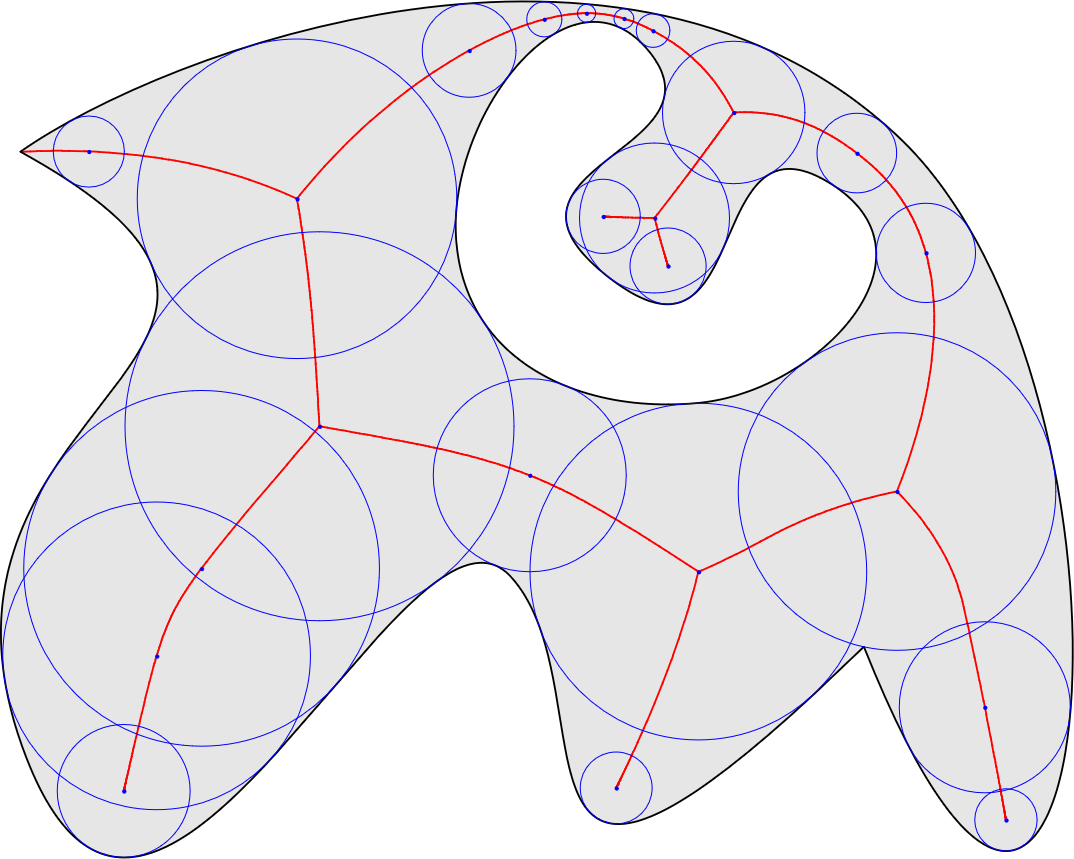
\includegraphics[scale=0.3]{images/median_axis.png}
    \caption{Construction de l'axe médian. Source: \cite{de2009fast}}
    \label{fig:median_axis}
\end{figure}

\subsubsection{Approches basées sur l'avancée de fronts}

Ces méthodologies s'apparentent à celles abordées pour la formation de maillages triangulaires. Une première méthode débute avec un maillage triangulaire puis définit des ensembles de fronts le long des arêtes de triangles de la frontière du domaine. Les triangles sont systématiquement combinés à ces fronts, progressant vers l'intérieur de la zone. Le front agit comme une division entre les quadrilatères déjà formés et les triangles qui doivent encore être combinés. Cette technique garantit un maillage entièrement quadrilatéral, à condition que le nombre initial d'arêtes de la frontière soit pair \cite{owen1999q}. D'autres méthodes se basent sur une approche directe. Le pavage présenté par Blacker et Stephenson \cite{blacker1991paving} consiste à former des rangées complètes d'éléments à partir de la frontière tout en progressant vers l'intérieur. White and Kinney ont avancé des améliorations à l'algorithme de pavage en préconisant l'insertion individuelle d'éléments plutôt que la création de rangées complètes \cite{white1997redesign}. Une alternative intéressante aux méthodes de pavage traditionnelle est l'algorithme Q-Morph. Il s'agit d'une méthode indirecte donc basée sur un maillage triangulaire initial permettant de maintenir des rangées d'éléments bien alignés et de réduire le nombre de nœuds irréguliers internes. Les différentes étapes de cette méthode sont les suivantes \cite{owen1999q}:\\

\begin{itemize}
    \item Maillage initial: initialement, la surface est triangulée en utilisant n'importe quelle méthode de triangulation de surface. Ce maillage devrait intégrer toute information de dimensionnement ou d'adaptativité. Le dimensionnement local pour le maillage quadrilatéral final suivra de près celui du maillage triangulaire.\\

    \item Définition du Front: le front initial est établi à partir des arêtes de la triangulation. Toute arête qui est adjacente à un seul triangle fait partie du front initial.\\

    \item Classification des arêtes de front: chaque arête dans le front est catégorisée en fonction de son état qui détermine comment l'arête sera finalement utilisée pour former un quadrilatère. Les états des arêtes frontales sont déterminés par les angles entre les arêtes adjacentes. Ces arêtes seront mises à jour et réorganisées au fur et à mesure que l'algorithme progresse.\\

    \item Traitement des arêtes frontales: chaque arête frontale est traitée individuellement pour construire un nouveau quadrilatère en utilisant les triangles du maillage triangulaire (voir Figure \ref{fig:step_front_advancing}).

    \begin{figure}[!h]
    \centering
    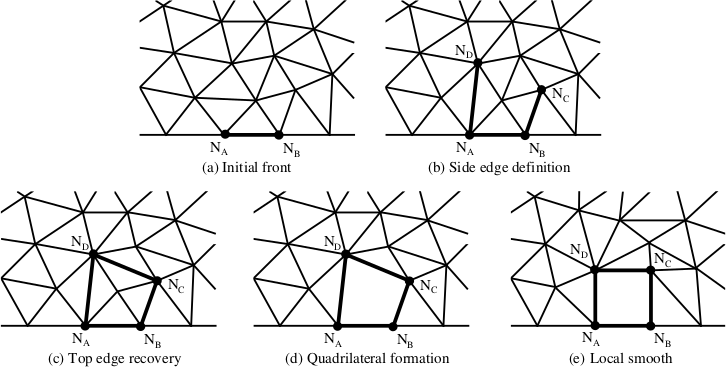
\includegraphics[scale=0.6]{images/step_front_advancing.png}
    \caption{Illustration du processus de génération d'un quadrilatère à partir d'une arête frontale. Source : \cite{owen1999q}.}
    \label{fig:step_front_advancing}
    \end{figure}

    \item Nettoyage topologique: la qualité des éléments est améliorée en effectuant des transformations locales sur les quadrilatères dans le but d'améliorer les valences individuelles des arêtes au niveau des nœuds du maillage.\\

    \item Lissage: une dernière étape de lissage est réalisée pour améliorer davantage la qualité des éléments.\\
\end{itemize}


\section{Maillages quadrilatéraux à partir de champs de croix}

Une méthode de génération de maillages quadrilatéraux intéressante repose sur les \emph{champs de croix}. Un champ de croix sur un domaine est une structure de champ qui attribue une \emph{croix} à presque chaque point du domaine, où une croix est un ensemble de vecteurs du fibré tangent. Elle est constitué d'un vecteur donné et de ses rotations avec un angle de $k\displaystyle\frac{\pi}{2}$, où $k \in \llbracket 0,3\rrbracket$. Les champs de croix sont utilisés pour la première fois dans les applications de graphisme informatique pour contrôler la mise en correspondance de surface pour le rendu non photoréaliste, la synthèse de textures et le ramaillage \cite{ray2008n, bommes2009mixed, nieser2011cubecover}.\\

\paragraph{Lien entre les champ de croix et les maillages quadrilatéraux:} une astuce particulièrement ingénieuse consiste à exploiter les lignes de champ d'un vecteur pour définir les quadrilatères d'un maillage quadrilatéral sur un domaine donné. Toutefois, pour que cela fonctionne, il est impératif de garantir que ces lignes de champ ne se croisent que sous un angle de $\frac{\pi}{2}$. C'est pourquoi l'utilisation d'un champ spécifique constitué de croix en chaque point du domaine est cruciale. L'avantage des champs de croix est de pouvoir représenter les caractéristiques des quadrilatères en deux dimensions. Dans \cite{beaufort2017computing}, les auteurs montrent que les sommets non réguliers d'un maillage quadrilatéral (les sommets qui ne sont pas adjacents à exactement quatre voisins) correspondent précisément aux points critiques d'un champ de croix. Ces points critiques du champ de croix peuvent également être liés à la caractéristique d'Euler de la surface maillée via la formule de Poincaré suivante:
$$
\sum_i index(x_i)=\chi,
$$
où $\chi=V-E+F$ désigne la caractéristique d'Euler, avec $V$ le nombre de sommets, $E$ le nombre d'arêtes et $F$ le nombre de faces.\\

Les méthodes de génération de maillage basées sur les champs de croix se décomposent en deux étapes principales à savoir la génération du champ de croix puis la construction du maillage quadrilatéral correspondant.

\paragraph{Géneration du champ de croix:} l'idée est de calculer un champ de croix le plus lisse possible afin de minimiser les variations brusques de l'orientation des quadrangles. 

Lorsqu'on aborde le cas d'une surface, l'approximation la plus optimale est obtenue en alignant les éléments selon les directions principales de courbure. Ainsi, il est préférable de générer des champs de croix qui suivent ces directions. Cette approche a été mise en œuvre dans des travaux tels que \cite{alliez2003anisotropic, marinov2004direct, kalberer2007quadcover}. Ce choix méthodologique présente l'avantage de créer des champs de croix attrayants qui s'harmonisent avec les propriétés inhérentes de la surface grâce à une méthode simple, ce qui a pour résultat que les singularités se forment naturellement aux points ombilicaux. Cependant, il convient de noter qu'il existe des zones étendues où la courbure normale se rapproche des valeurs de courbure principales, engendrant une définition moins précise du champ de croix \cite{fogg2015automatic}.

Un autre critère necessaire pour les simulations est le respect de la frontiere du domaine lors de la discritisation. Pour se faire, il est necessaire de prendre en compte des contraintes d'alignements par rapport aux frontieres des elements quadrangulaires. Généralement un ensemble d'arêtes d'un maillage triangulaire ou d'une géométrie de CAO est utilisé comme condition aux limites afin de générer un champ de croix aligné avec ces  arêtes. c'est ce qui est mis en oeuvre dans \cite{kowalski2013pde, palacios2007rotational} où un champ vectoriel de représentation est résolu via une équation de la chaleur avec des conditions aux limites de Dirichlet donné par la normale aux bords. Cette méthode ne peut cependant pas traiter facilement les surfaces courbes et elle n'est pas adaptée pour s'ajuster aux tailles et directions d'élements cibles \cite{fogg2015automatic}. \cite{bommes2009mixed} proposent une formulation d`optimisation linéaire à variables mixtes, résolue à l'aide d'un solveur adaptatif. Des contraintes directionnelles éparses permettent de déterminer automatiquement le nombre approprié, le type et la position des singularités. Dans \cite{bunin2008towards}, Bunin résoud directement un probleme de Poisson inverse avec une distribution de sources ponctuelles représentant les irrégularité du maillage. La méthode est attrayante d'un point de vue théorique et montre des résultats impressionnants. Cependant, elle semble contenir des étapes nécessitant un réglage minutieux et des sensibilités élevées aux erreurs numériques sont rapportées pour les problèmes avec un grand nombre de singularités \cite{fogg2015automatic}.


\paragraph{Génération d'un maillage correspondant au champ de croix calculé:}

Une stratégie initiale pour générer des maillages quadrilatéraux à partir de champs de repères croisés consiste en la paramétrisation. Cette méthode implique la création d'une transformation du domaine à mailler vers un espace paramétrique, où l'application d'une grille régulière au domaine transformé devient possible. Inverser cette transformation permet alors de dériver un maillage quadrilatéral du domaine, aligné sur ses contours. L'avantage majeur de cette approche réside dans sa capacité à gérer des discontinuités dans la transformation, ce qui en fait une méthode adaptée pour traiter des singularités \cite{reberol2018maillages}. Il existe des algorithmes robustes basés sur des paramétrisations globales \cite{ray2006periodic, kalberer2007quadcover, myles2014robust, campen2015quantized}. L'élément clé de ces algorithmes est la décomposition du domaine en des cartes de forme quadrilatère en découpant le domaine le long d'un graphe en suivant par exemple les lignes de champ du champ de croix. Ainsi dans \cite{ray2006periodic}, les auteurs paramétrisent des surfaces de genre arbitraire avec des fonctions de potentiel périodiques guidées par deux champs vectoriels d'entrée orthogonaux. Cela conduit à une paramétrisation continue à l'exception des points singuliers sur la surface. Ces régions singulières sont détectées et reparamétrées par la suite. L'algorithme QuadCover \cite{kalberer2007quadcover} calcule automatiquement une paramétrisation globale dont les lignes paramétriques sont guidées par le champ de croix. La méthode génère des maillages quadrilatéraux de bonne qualité avec des éléments de petites tailles mais gère difficilement des tailles de maillages grossières.

Outre la paramétrisation, une autre méthode consiste à générer une partition du domaine en utilisant le champ de croix.  Dans \cite{kowalski2013pde}, les auteurs construisent ce partitionnement en traçant des lignes de séparation à travers le champ croisé. Les champs croisés sont utilisés pour capturer les caractéristiques d'orientation des quadrilatères, permettant ainsi la génération d'une partition bien définie du domaine en sous-domaines. Il est ensuite nécessaire de résoudre un problème d'assignation d'intervalles pour le maillage quadrilatère consistant à attribuer à chaque courbe le nombre d'arêtes (intervalles) en lesquelles elle doit être subdivisée, de manière à ce que chaque surface  puisse être maillée \cite{hohring1997mesh, mitchell2000high, mitchell2014simple}. Par exemple, mailler une surface rectangulaire avec des quadrilatères nécessite que les courbes sur les côtés opposés contiennent exactement le même nombre d'arêtes.


\section{Objectif de la thèse}


L'objectif de cette thèse est d'amener de nouvelles solutions pour gagner en performance lors de résolutions numériques d'équations aux dérivées partielles (en particulier pour l'électromagnétisme, la mécanique des fluides, l'élasticité, etc.).

Dans un premier temps, nous nous intéressons à la possibilité de construire un maillage quadrilatéral à partir d'un champ de croix fournit par un utilisateur. En effet, les champs de croix générer en propageant la normale extérieur à l'intérieur du domaine \cite{kowalski2013pde} produisent une distribution de singularités pouvant conduire à un partitionnement invalide ou non souhaité. Un problème notable survient dans les domaines extrêmement étirés, tandis qu'une autre préoccupation concerne les formes de partitionnement qui entraînent des tailles de cellules très non uniformes (voir figure \ref{fig:dom_etire_mesh_inhomogene}).

\begin{figure}[!h]
    \centering
    %\includegraphics[scale=0.5]{img/cercle non_homogene.pdf}
    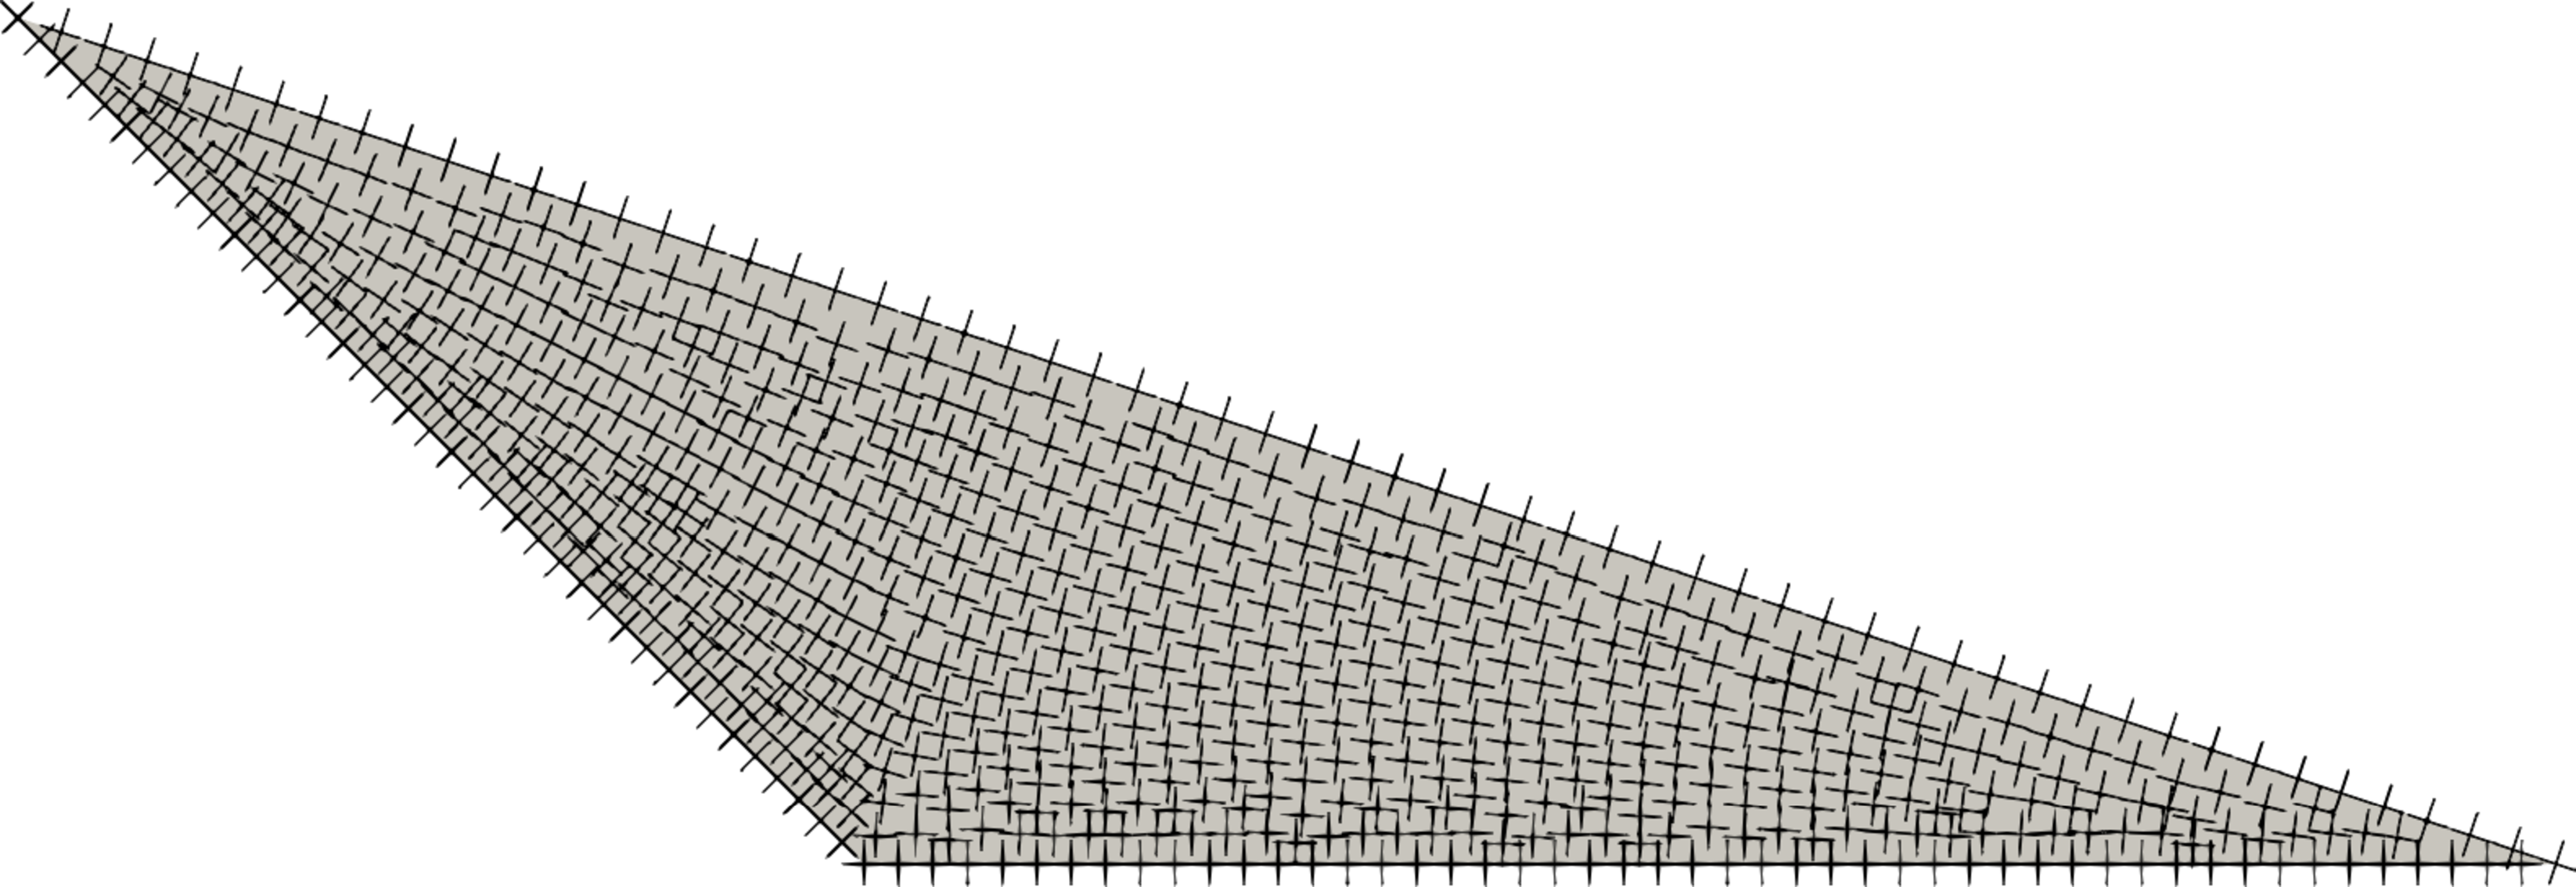
\includegraphics[scale=0.18]{images/stretch.pdf}
    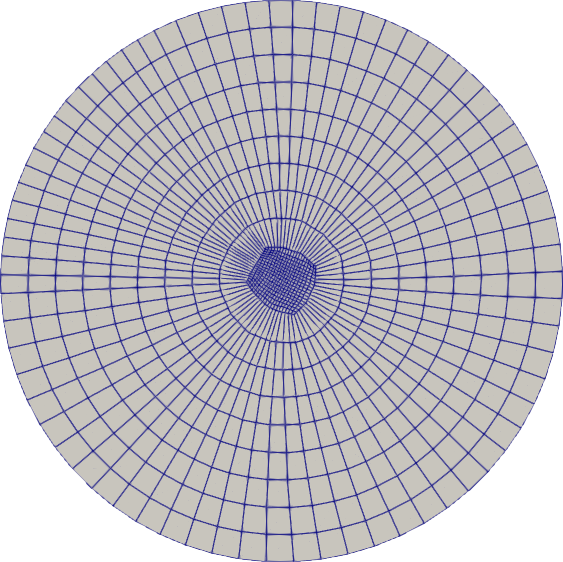
\includegraphics[scale=0.22]{images/new_cercle.png}
    \caption{Gauche: Champ de croix sur un domaine étiré; Droite: Maillage non-homogène d'un disque.}
    \label{fig:dom_etire_mesh_inhomogene}
\end{figure}

Pour surmonter ces problèmes, il est essentiel de focaliser notre attention sur le contrôle à la fois du type et de l'emplacement des points singuliers dans le champ croisé. À cet égard, Jezdimirović et al. \cite{jezdimirovic2021quad} ont présenté un algorithme qui repose sur un modèle de singularité spécifié par l'utilisateur en entrée, pouvant inclure des singularités de grande valence. De même, Alexis Macq et al. \cite{macq2020ginzburg} ont élaboré une formulation basée sur l'énergie de Ginzburg-Landau, qui permet d'imposer des singularités internes en les substituant par de petits trous pratiqués dans le domaine. Dans le cadre de cette thèse, nous explorons une approche qui prend racine dans la sélection d'un champ de croix répondant à un ensemble spécifique de propriétés. Ensuite, nous cherchons à aligner ce champ par rapport aux frontières du domaine de calcul. Par la suite nous élargissons cette approche aux domaines non simplement connexes, dans le but de pouvoir tenir compte des situations où le domaine est constitué de plusieurs matériaux distincts (multi-matériau).

Lors des simulations numériques, prendre en compte les conditions aux limites est une étape fondamentale. Pour ce faire, il est impératif d'introduire des points de passage dans le maillage, créant ainsi des segments de frontières qui correspondent à la localisation de ces conditions aux limites dans la structure du maillage. Dans cette optique, notre intention est d'enrichir le processus mentionné précédemment, qui concerne le champ croisé, en intégrant la prise en compte de ces points de passage, qui se manifestent sous forme de singularités de bord.

Nous étendons enfin cette approche aux surfaces courbes, et à l'instar de \cite{viertel2019approach}, nous établissons un cadre théorique pour analyser la régularité des champs croisés, tout en présentant une série d'opérations qui facilitent leur manipulation.

\section{Organisation du manuscrit}

 Ce mémoire est organisé de la manière suivante:\\

 Dans le \textbf{\color{blue!50!black}{Chapitre 1}}

\newpage
\section{Communications issues de la thèse}

Les travaux de recherche effectués ont mené aux communications suivantes:

\subsubsection{Article soumis}

\subsubsection{Proceeding}

\subsubsection{Communications orales dans des conférences internationales}

\begin{itemize}
    \item \textit{Quadrilateral mesh create from a given cross field}, 10th International Conference on Curves and Surfaces, Arcachon, France, 20-24 Juin 2022.\\
    \item \textit{Quadrilateral mesh of non-simply connected domain and non-planar surfaces from a given cross-field}, The SIAM International Meshing Roundtable Workshop 2023 (SIAM IMR 2023), Amsterdam, Netherlands, 06-09 Mars 2023.
\end{itemize}

\subsubsection{Communications orales dans des conférences nationales}

\begin{itemize}
    \item \textit{Génération de maillages quadrilatéraux à partir de champs de croix donnés}, Journées Ondes du Sud-Ouest 2023 (JOSO 2023), Toulouse, France, 14-16 Mars 2023.\\
    \item \textit{Méthode de maillage en quadrilatères par résolution d'EDP}, Laboratoire de Mathématiques Appliquées à l'Aéronautique et au Spatial (LMA2S), Toulouse, France, Mars 2021.
\end{itemize}



\subsubsection{Communications dans des séminaires doctorants}


\subsubsection{Logiciels}




\chapter{Génération de maillages quadrilatéraux à partir de champs de croix prescrits}
\label{chap:theoritical}
\minitoc

\[\]

Dans le chapitre précédent, nous avons annoncé notre intention d'améliorer la topologie des maillages quadrilatéraux générés par la méthode de partitionnement basée sur les champs de croix, afin de remédier aux différentes limitations mentionnées. Il est important de noter que les champs de croix présentent les mêmes types de singularités que l'on observe dans les maillages quadrilatéraux générés. Par conséquent, la génération d'un maillage quadrilatéral très régulier ou présentant d'autres propriétés est étroitement liée à la génération d'un champ de croix possédant les propriétés souhaitées. À partir de cette observation, nous choisissons d'initier la méthode de partitionnement avec un champ de croix prédéfini, puis, au besoin, de le modifier pour qu'il puisse être utilisé dans le processus de partitionnement du domaine de calcul. Plusieurs questions se posent alors : quel champ choisir? quelle devrait être sa régularité? combien de singularités doit-il contenir? et de quel type doivent-elles être? Toutes ces questions soulignent l'importance de bien définir le concept de champ de croix et d'étudier de manière plus approfondie ses propriétés.

Dans ce chapitre, nous établissons un cadre théorique exhaustif et mettons à disposition une variété d'outils pour la manipulation des champs de croix. Nous prposons des définitions tels que l'angle d'une croix, l'indice d'un point dans un champ de croix, ainsi que de ligne de champ dans un champ de croix. Ensuite, nous abordons la méthode de partitionnement proprement dite. À cet effet, nous présentons différents algorithmes élaborés pour les géométries tant simplement connexes que non simplement connexes, ainsi que diverses opérations permettant d'ajuster un champ de croix donné en fonction du domaine à mailler. Enfin, nous exposons un ensemble de résultats qui justifient les algorithmes présentés et garantissent leur efficacité.



\section{Cadre théorique}

Dans cette section, nous présentons le concept de champ de croix défini sur un domaine donné et explorons quelques-unes de ses propriétés clés. Considérons $\Omega$ comme un domaine borné et fermé de $\mathbb{R}^2$ ayant une frontière $\partial\Omega$ lisse par morceaux.

\subsection{Champ de croix}

Soit $\mathbb{S}^1$ la sphère unité de $\mathbb{R}^2$ définie par $\mathbb{S}^1=\{(x,y)\in\mathbb{R}^2~|~x^2+y^2=1\}$ et soit $\mathcal{Q}$ le groupe de symétrie quadrilatérale défini comme l'ensemble des rotations d'angle $k\pi/2$, $k\in\{0, 1, 2, 3\}$.

\begin{definition}[\cite{beaufort2017computing}]
\label{def:croix}
  Une croix $\mathbf{c}$ est un élément de $\mathbf{C}:=\mathbb{S}^1/\mathcal{Q}\cup\{0\}$.
\end{definition}

En d'autres termes, $\mathbf{c}$ représente une classe d'équivalence dont les éléments, nommés branches de la croix, répondent à la relation suivante (voir figure \ref{fig:croix}):

\begin{equation}
\label{eq:croix}
\forall~(c^1, c^2)\in\mathbf{c}\times\mathbf{c},~\exists~m\in\mathbb{Z},~c^1=\mathbf{R}\left(\frac{m\pi}{2}\right)c^2,
\end{equation}
où $\mathbf{R}(.)$ est l'opérateur de rotation défini par:
\begin{equation}
\label{eq:matricerotation}
\mathbf{R}(.)=
\begin{pmatrix}
\cos(.) & -\sin(.) \\
\sin(.) & \cos(.) \\
\end{pmatrix}.
\end{equation}

\begin{figure}[!h]
  \centering
  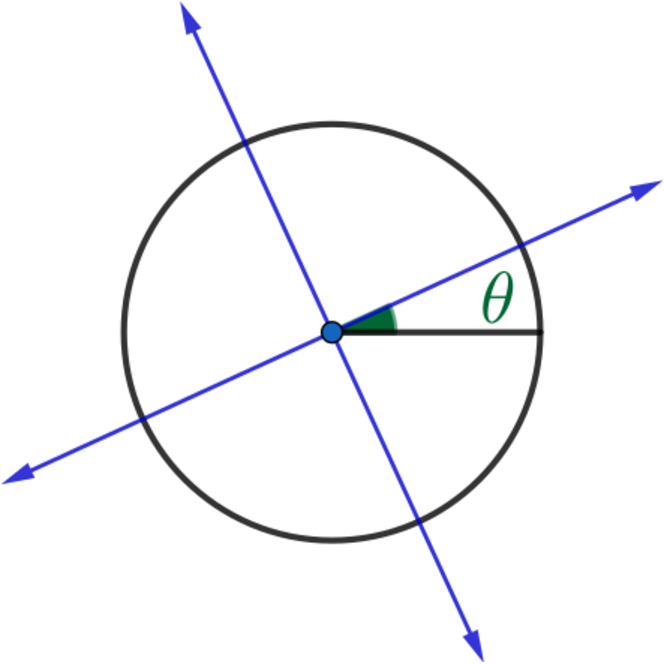
\includegraphics[scale=0.5]{images/cross.pdf}
  \caption{Illustration d'une croix.}
  \label{fig:croix}
\end{figure}

Un champ de croix $\bar{u}$ défini sur $\Omega$ est une fonction qui associe à chaque point $p\in\Omega$ une croix $\bar{u}(p)\in\mathbf{C}$.

\begin{definition}
    Si $\bar{u}(p)=0$ pour $p\in\Omega$ alors on dit que $p$ est un \emph{point singulier} de $\bar{u}$.
\end{definition}

Dans toute la suite, nous désignerons par  $\mathcal{S}_{\bar{u}}:={\bar{u}}^{-1}(\{0\})$ l'ensemble des points singuliers de $\bar{u}$.

\begin{definition}%[ $\mathcal{C}^1$ cross field]
\label{def:cont}
$\bar{u}$ est de classe $\mathcal{C}^1$ en un point $p$ s'il existe une application $\pi_{\bar{u}}$ dans un voisinnage $V_p$ de $p$ tel que $\pi_{\bar{u}}\in\mathcal{C}^1(V_p)$ et $\pi_{\bar{u}}(q)\in\bar{u}(q)$ pour tout $q\in V_p$.
\end{definition}

Comme toutes les composantes de $\bar{u}$ sont obtenues par rotations d'angles $m\pi/2$, où $m\in\mathbb{Z}$, la propriété énoncée précédemment peut être reformulée en tant qu'exigence de continuité $C^1$ pour toutes les composantes dans le voisinage de $p$.

\begin{definition}
\label{def:presqueC1}
    $\bar{u}$ est un champ de croix \emph{presque-$\mathcal{C}^1$} si $Card(\mathcal{S}_{\bar{u}})<\infty$ et si $\bar{u}$ est de classe $\mathcal{C}^1$ en tout point $p\in\Omega\backslash\mathcal{S}_{\bar{u}}$ (où $Card(\mathcal{S}_{\bar{u}})$ est le cardinal de $\mathcal{S}_{\bar{u}}$).
\end{definition}


Le résultat suivant établit la régularité des champs de croix construits à partir de fonctions de représentation \cite{kowalski2013pde, viertel2019approach} puis définit l'opération et la régularité de la rotation d'un champ de croix par rapport à un champ d'angle (voir figure \ref{fig:repr_to_cross} et figure \ref{fig:rot_cross}).

\begin{proposition}
\label{prop:cont1}
\[\]
\vspace{-1cm}
\begin{enumerate}
\item Soit $f : \Omega \rightarrow \mathbb{R}^2$ un champ de vecteur de classe $\mathcal{C}^1$ sauf en un nombre fini de point où $f$ s'annule. La fonction $\bar{u}$ définie pour tout $p\in\Omega$ par :
\begin{equation}
    \bar{u}(p) =
\left\{
    \begin{array}{lc}
        \displaystyle\left\{\mathbf{R}\left(\frac{m\pi}{2}\right)\frac{f(p)}{\left\|f(p)\right\|},~ m\in \mathbb{Z}\right\} &\text{ si }f(p)\neq 0,\\\\
        0& \text{sinon}
    \end{array}
\right.
\label{eq:repr_to_cross}
\end{equation}
est un champ de croix presque-$\mathcal{C}^1$ sur $\Omega$.

\item Soit $\bar{u}$ un champ de croix sur $\Omega$ et $\theta : \Omega \rightarrow \mathbb{R}$ une fonction définie sur $\Omega$. Alors l'application $\bar{v}:p\mapsto \bar{v}(p)=\mathbf{R}(\theta(p))\bar{u}(p):=\{\mathbf{R}(\theta(p)) u,~u\in \bar{u}(p)\}$ est un champ de croix sur $\Omega$. De plus $\mathcal{S}_{\bar{u}}=\mathcal{S}_{\bar{v}}$ et si $\theta$ est de classe $\mathcal{C}^1$ en $p\in\Omega$ (resp. sur $\Omega$) alors $\bar{v}$ est de classe $\mathcal{C}^1$ en $p$ (resp. presque-$\mathcal{C}^1$ sur $\Omega$) si et seulement si $\bar{u}$ l'est.
\end{enumerate}
\end{proposition}

\begin{proof}
\[\]
\vspace{-1cm}
\begin{enumerate}
\item Pour tout $p\in\Omega$, si $\bar{u}(p)\neq 0$ alors pour tout $(u^1, u^2)\in\bar{u}(p)\times\bar{u}(p)$, il existe $m_1,m_2\in\mathbb{Z}$ tel que $u_1=\mathbf{R}(\frac{m_1\pi}{2})\frac{f(p)}{\left\|f(p)\right\|}$ et $u_2=\mathbf{R}(\frac{m_2\pi}{2})\frac{f(p)}{\left\|f(p)\right\|}$. On a donc $u^1=\mathbf{R}(\frac{(m_1-m_2)\pi}{2})u^2$ ce qui implique que $\bar{u}(p)\in\mathbf{C}\backslash\{0\}$. Autrement, $\bar{u}(p)=0$. Il vient donc que $\bar{u}$ est un champ de croix.

Soit $F$ l'ensemble des points où $f$ s'annule. L'application $\pi_{\bar{u}}:=f/\|f\|^{-1}$ définie sur $\Omega\backslash F$ est de classe $\mathcal{C}^1$ puisque $f$ l'est. De plus, pour tout $p\in\Omega\backslash F$, $\pi_{\bar{u}}(p)\in\bar{u}(p)$ donc $\bar{u}$ est de classe $\mathcal{C}^1$ sur $\Omega\backslash F$. Par définition on a donc $\mathcal{S}_{\bar{u}}=F$ de cardinal fini, donc $\bar{u}$ est un champ de croix presque-$\mathcal{C}^1$ sur $\Omega$.\\

\item Soit $p\in\Omega$. Si $\bar{u}(p)=0$ alors $\bar{v}(p)=0$, sinon $\bar{u}(p)\in\mathbf{C}\backslash\{0\}$ ce qui implique que $\bar{v}(p)\in\mathbf{C}\backslash\{0\}$. En effet, soit $(v^1, v^2)\in\bar{v}(p)\times\bar{v}(p)$. Par définition, il existe $(u^1, u^2)\in\bar{u}(p)\times\bar{u}(p)$ tel que $v^1=\mathbf{R}(\theta)u^1$ et $v^2=\mathbf{R}(\theta)u^2$. Or $\bar{u}(p)\in\mathbf{C}\backslash\{0\}$, donc il existe $m\in\mathbb{Z}$ tel que $u^1=\mathbf{R}\left(\frac{m\pi}{2}\right)u^2$. Ainsi:
$$
\mathbf{R}(\theta)u^1=\mathbf{R}(\theta)\mathbf{R}\left(\frac{m\pi}{2}\right)u^2,\mbox{ et donc }
v^1=\mathbf{R}\left(\frac{m\pi}{2}\right)v^2.
$$
Ce qui implique que $\bar{v}(p)\in\mathbf{C}\backslash\{0\}$. Autrement dit, $\bar{v}$ est un champ de croix sur $\Omega$. De plus $\mathcal{S}_{\bar{u}}=\mathcal{S}_{\bar{v}}$ puisque pour tout $p\in\Omega$, on a:
$$\bar{v}(p)=\{0\} \Leftrightarrow \left(\forall u\in \bar{u}(p),~\mathbf{R}(\theta(p)) u=0\right)\Leftrightarrow \left(\forall u\in \bar{u}(p),~u=0\right) \Leftrightarrow \bar{u}(p)=\{0\}.$$
Maintenant considérons que $\theta$  et $\bar{u}$ soient de classe $\mathcal{C}^1$ au voisinage de $p\in\Omega$. Par définition, il existe une application $\pi_{\bar{u}}$ de classe $\mathcal{C}^1$ dans un voisinnage $V_p$ de $p$. $\theta$ étant de classe $\mathcal{C}^1$, l'application $\pi_{\bar{v}}:=\mathbf{R}(\theta)\pi_{\bar{u}}$ est de classe $\mathcal{C}^1$ sur $V_p$. De plus, pour tout $q\in V_p$, $\pi_{\bar{v}}(q)=\mathbf{R}(\theta(q))\pi_{\bar{u}}(q)$ et comme $\pi_{\bar{u}}(q)\in\bar{u}(q)$ on a par définition $\pi_{\bar{v}}(q)\in\bar{v}(q)$. En conclusion, $\bar{v}$ est de classe $\mathcal{C}^1$ au voisinage de $p$.\\
Réciproquement, si $\bar{v}$ est de classe $\mathcal{C}^1$ au voisinage de $p\in\Omega$, alors par définition il existe une application $\pi_{\bar{v}}$ de classe $\mathcal{C}^1$ dans un voisinnage $V_p$ de $p$. $\theta$ étant de classe $\mathcal{C}^1$, l'application $\pi_{\bar{u}}:=\mathbf{R}(-\theta)\pi_{\bar{v}}$ est de classe $\mathcal{C}^1$ sur $V_p$. De plus, pour tout $q\in V_p$, $\pi_{\bar{u}}(q)=\mathbf{R}(-\theta(q))\pi_{\bar{v}}(q)$. Or $\pi_{\bar{v}}(q)\in\bar{v}(q)$ donc par définition il existe $u\in\bar{u}(q)$ tel que $\pi_{\bar{v}}(q)=\mathbf{R}(\theta(q))u$. On a donc :
$$
\pi_{\bar{u}}(q)=\mathbf{R}(-\theta(q))\mathbf{R}(\theta(q))u=u\Longrightarrow\pi_{\bar{u}}\in\bar{u}(q).
$$
En conclusion, $\bar{u}$ est de classe $\mathcal{C}^1$ au voisinage de $p$.\\
Pour finir, puisque $\mathcal{S}_{\bar{u}}=\mathcal{S}_{\bar{v}}$ alors $\bar{u}$ est un champ de croix presque-$\mathcal{C}^1$ sur $\Omega$ si et seulement si $\bar{v}$ est un champ de croix presque-$\mathcal{C}^1$ sur $\Omega$.
\end{enumerate}
\end{proof}

\begin{figure}[h!]
  \centering
  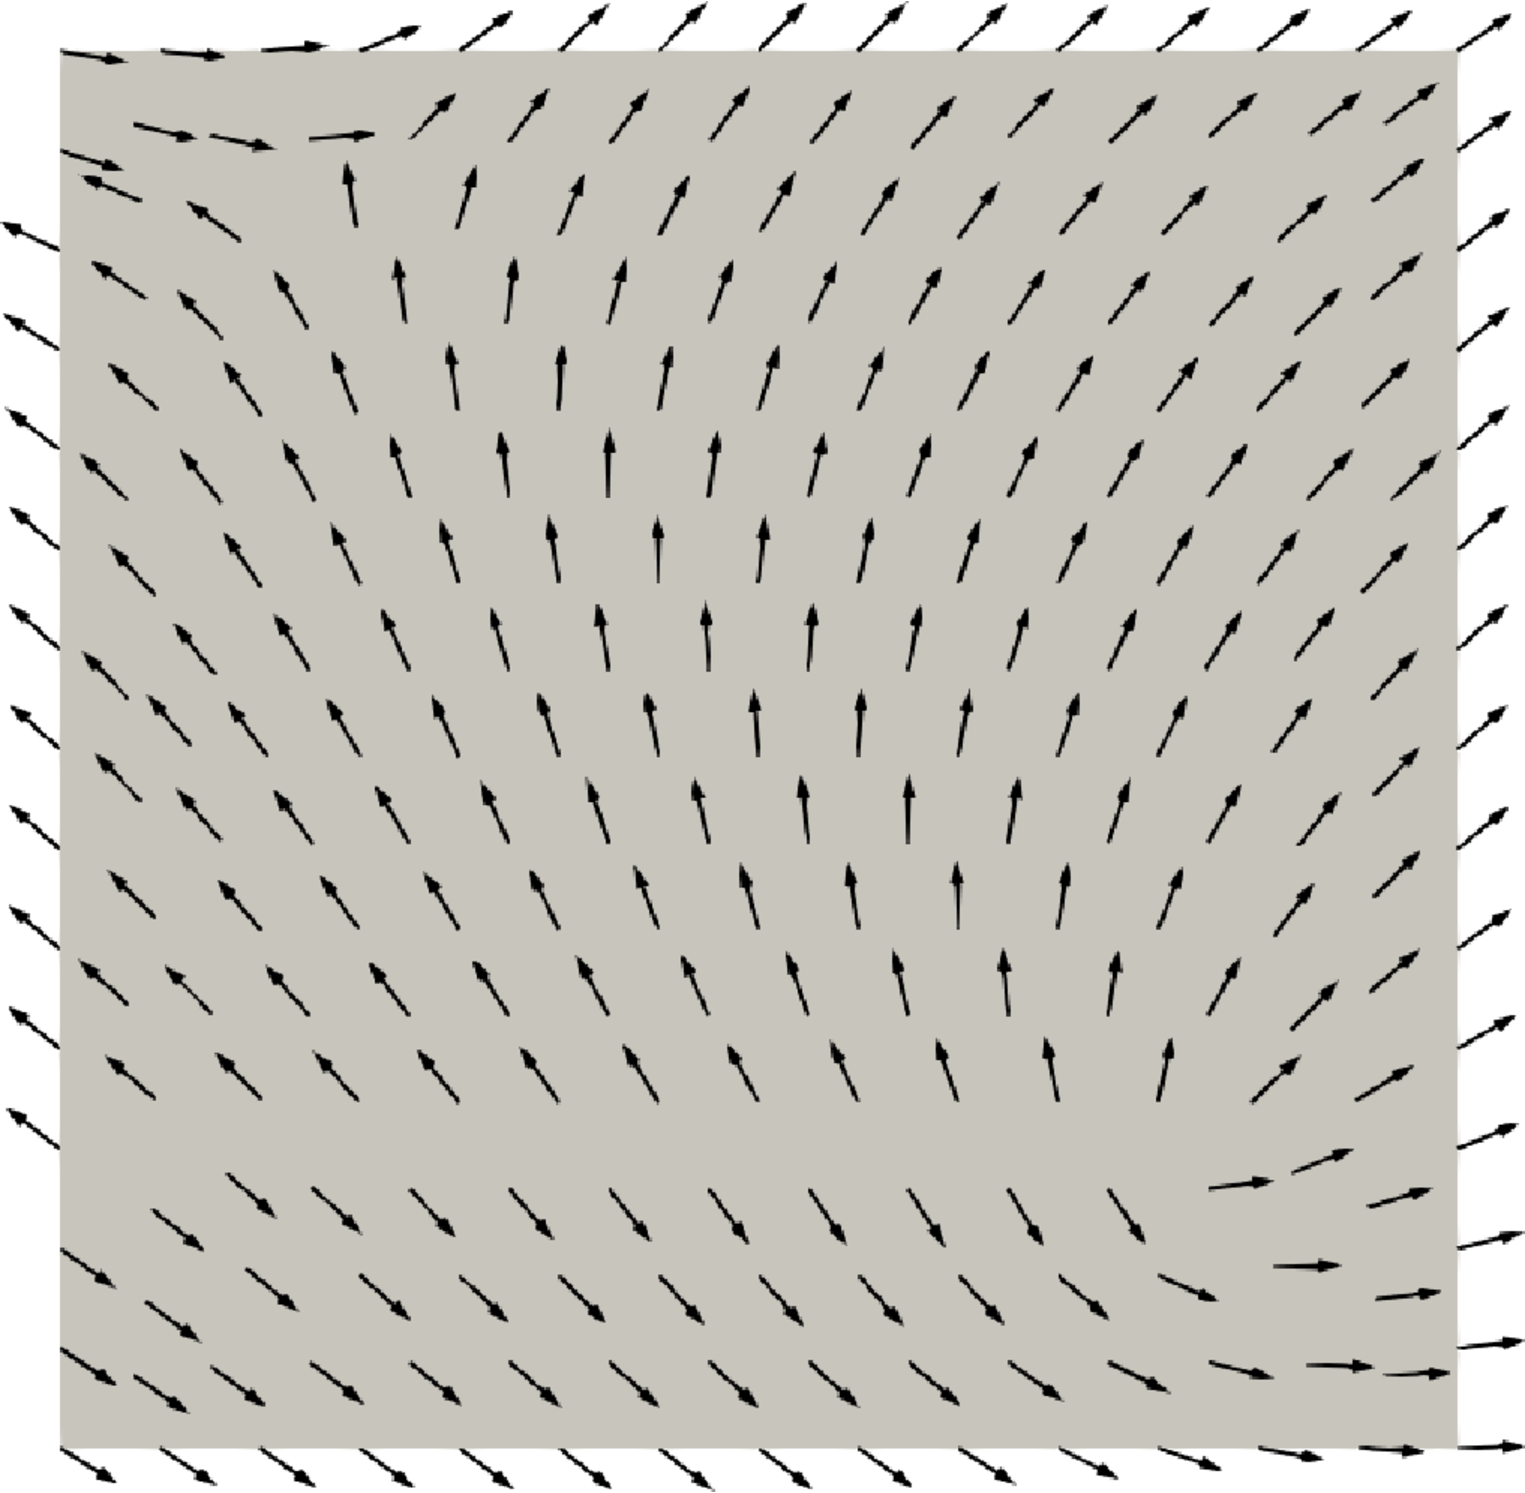
\includegraphics[scale=0.26]{images/repre_field.pdf}
  \hfill
  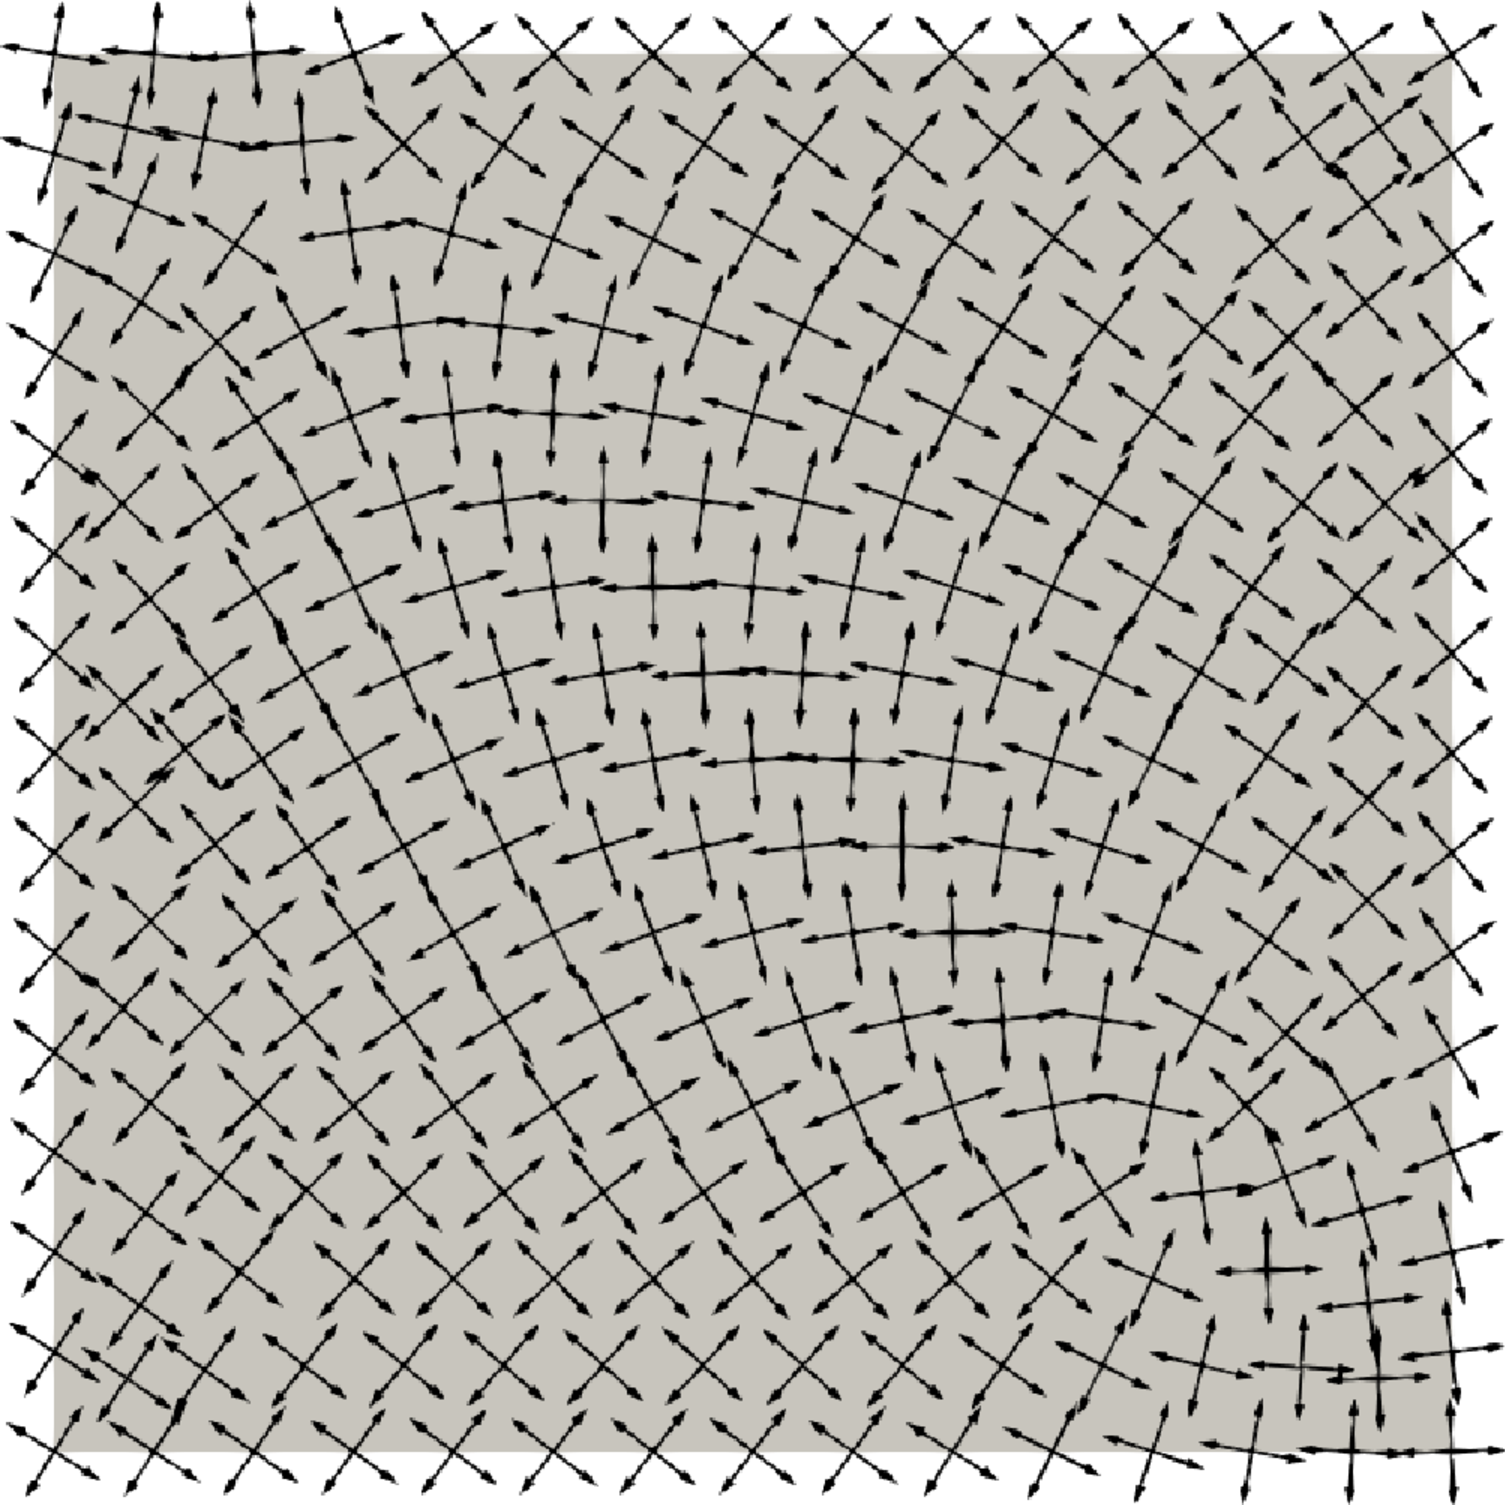
\includegraphics[scale=0.26]{images/cross_from_repre_field.pdf}
  \caption{Illustration d'un champ de représentation (en gauche) et du champ de croix associé (à droite).}
  \label{fig:repr_to_cross}
\end{figure}

\begin{figure}[h!]
  \centering
  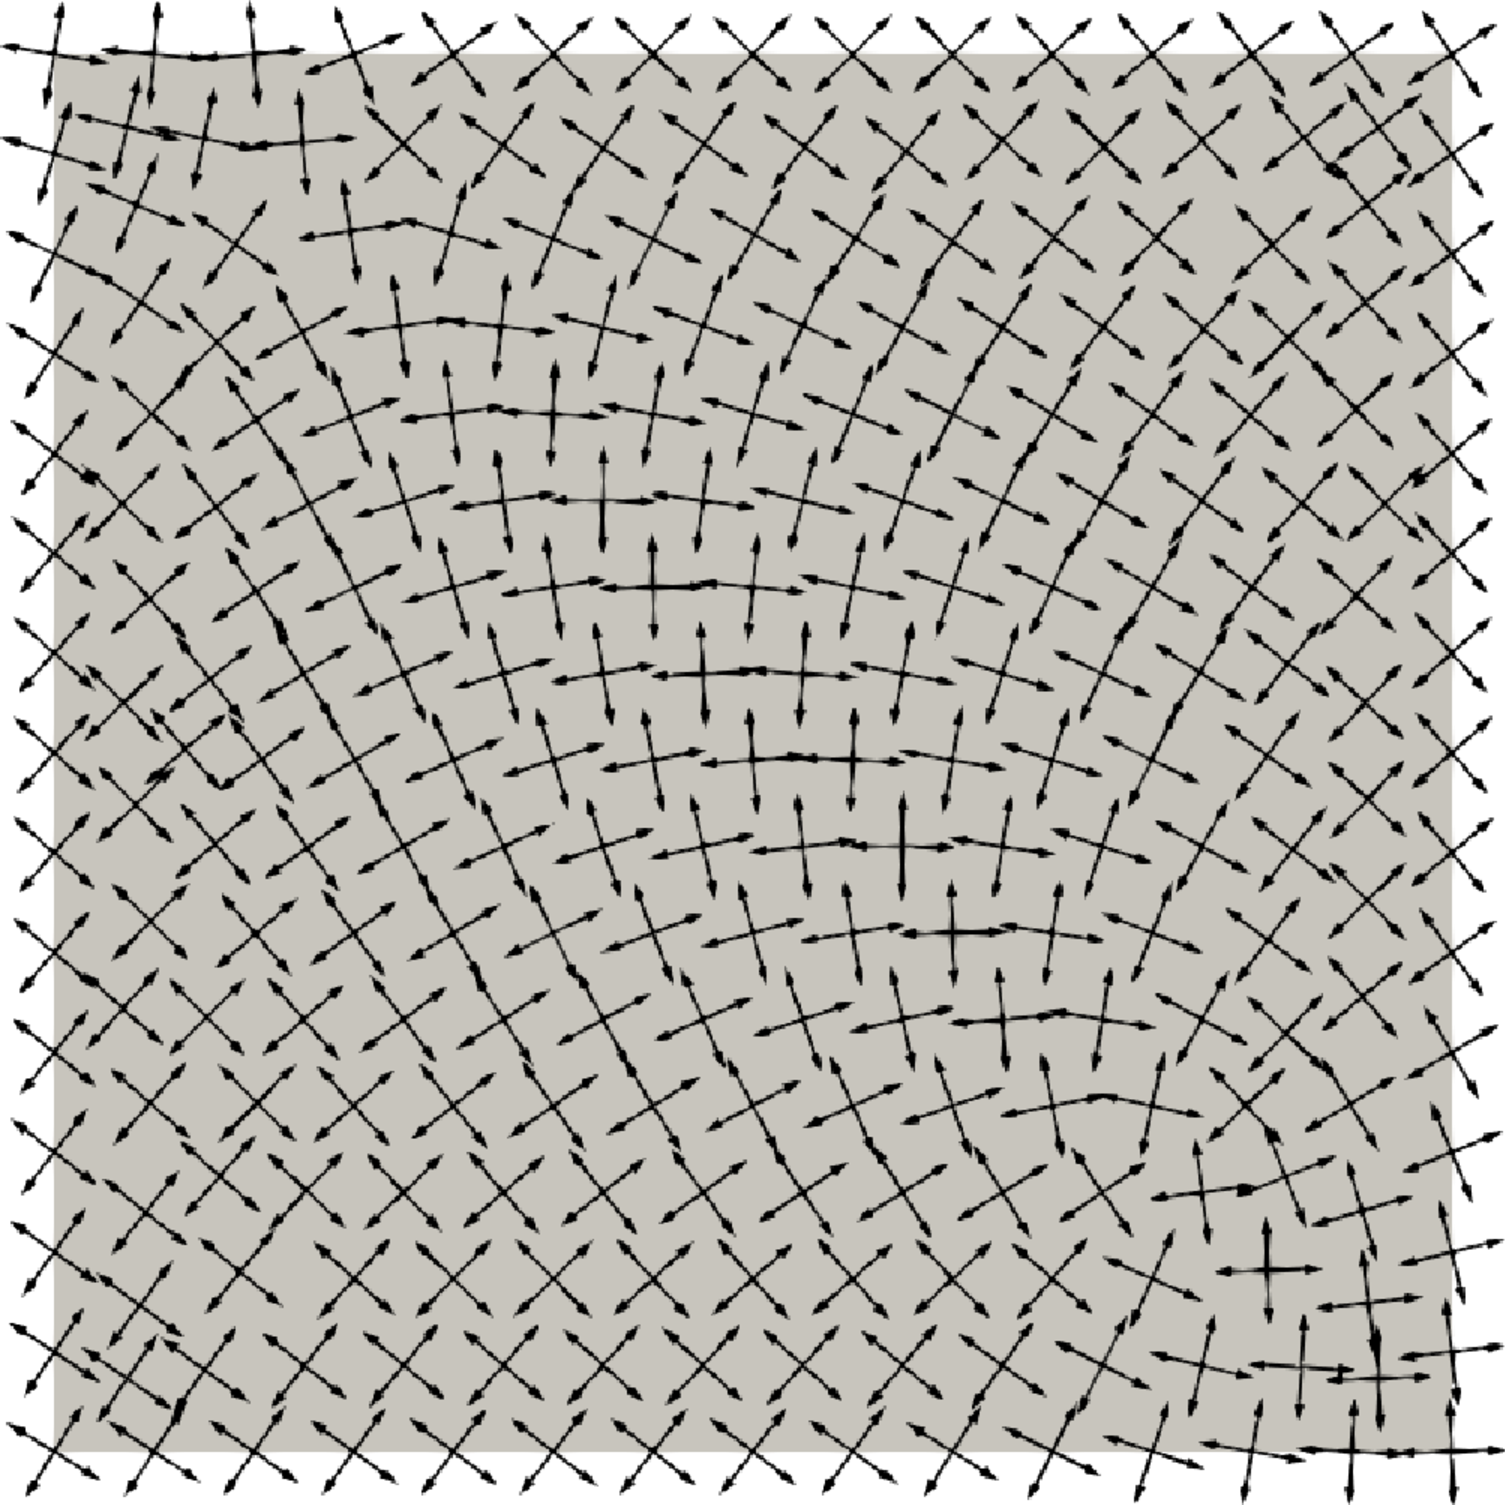
\includegraphics[scale=0.171]{images/cross_from_repre_field.pdf}
  \hfill
  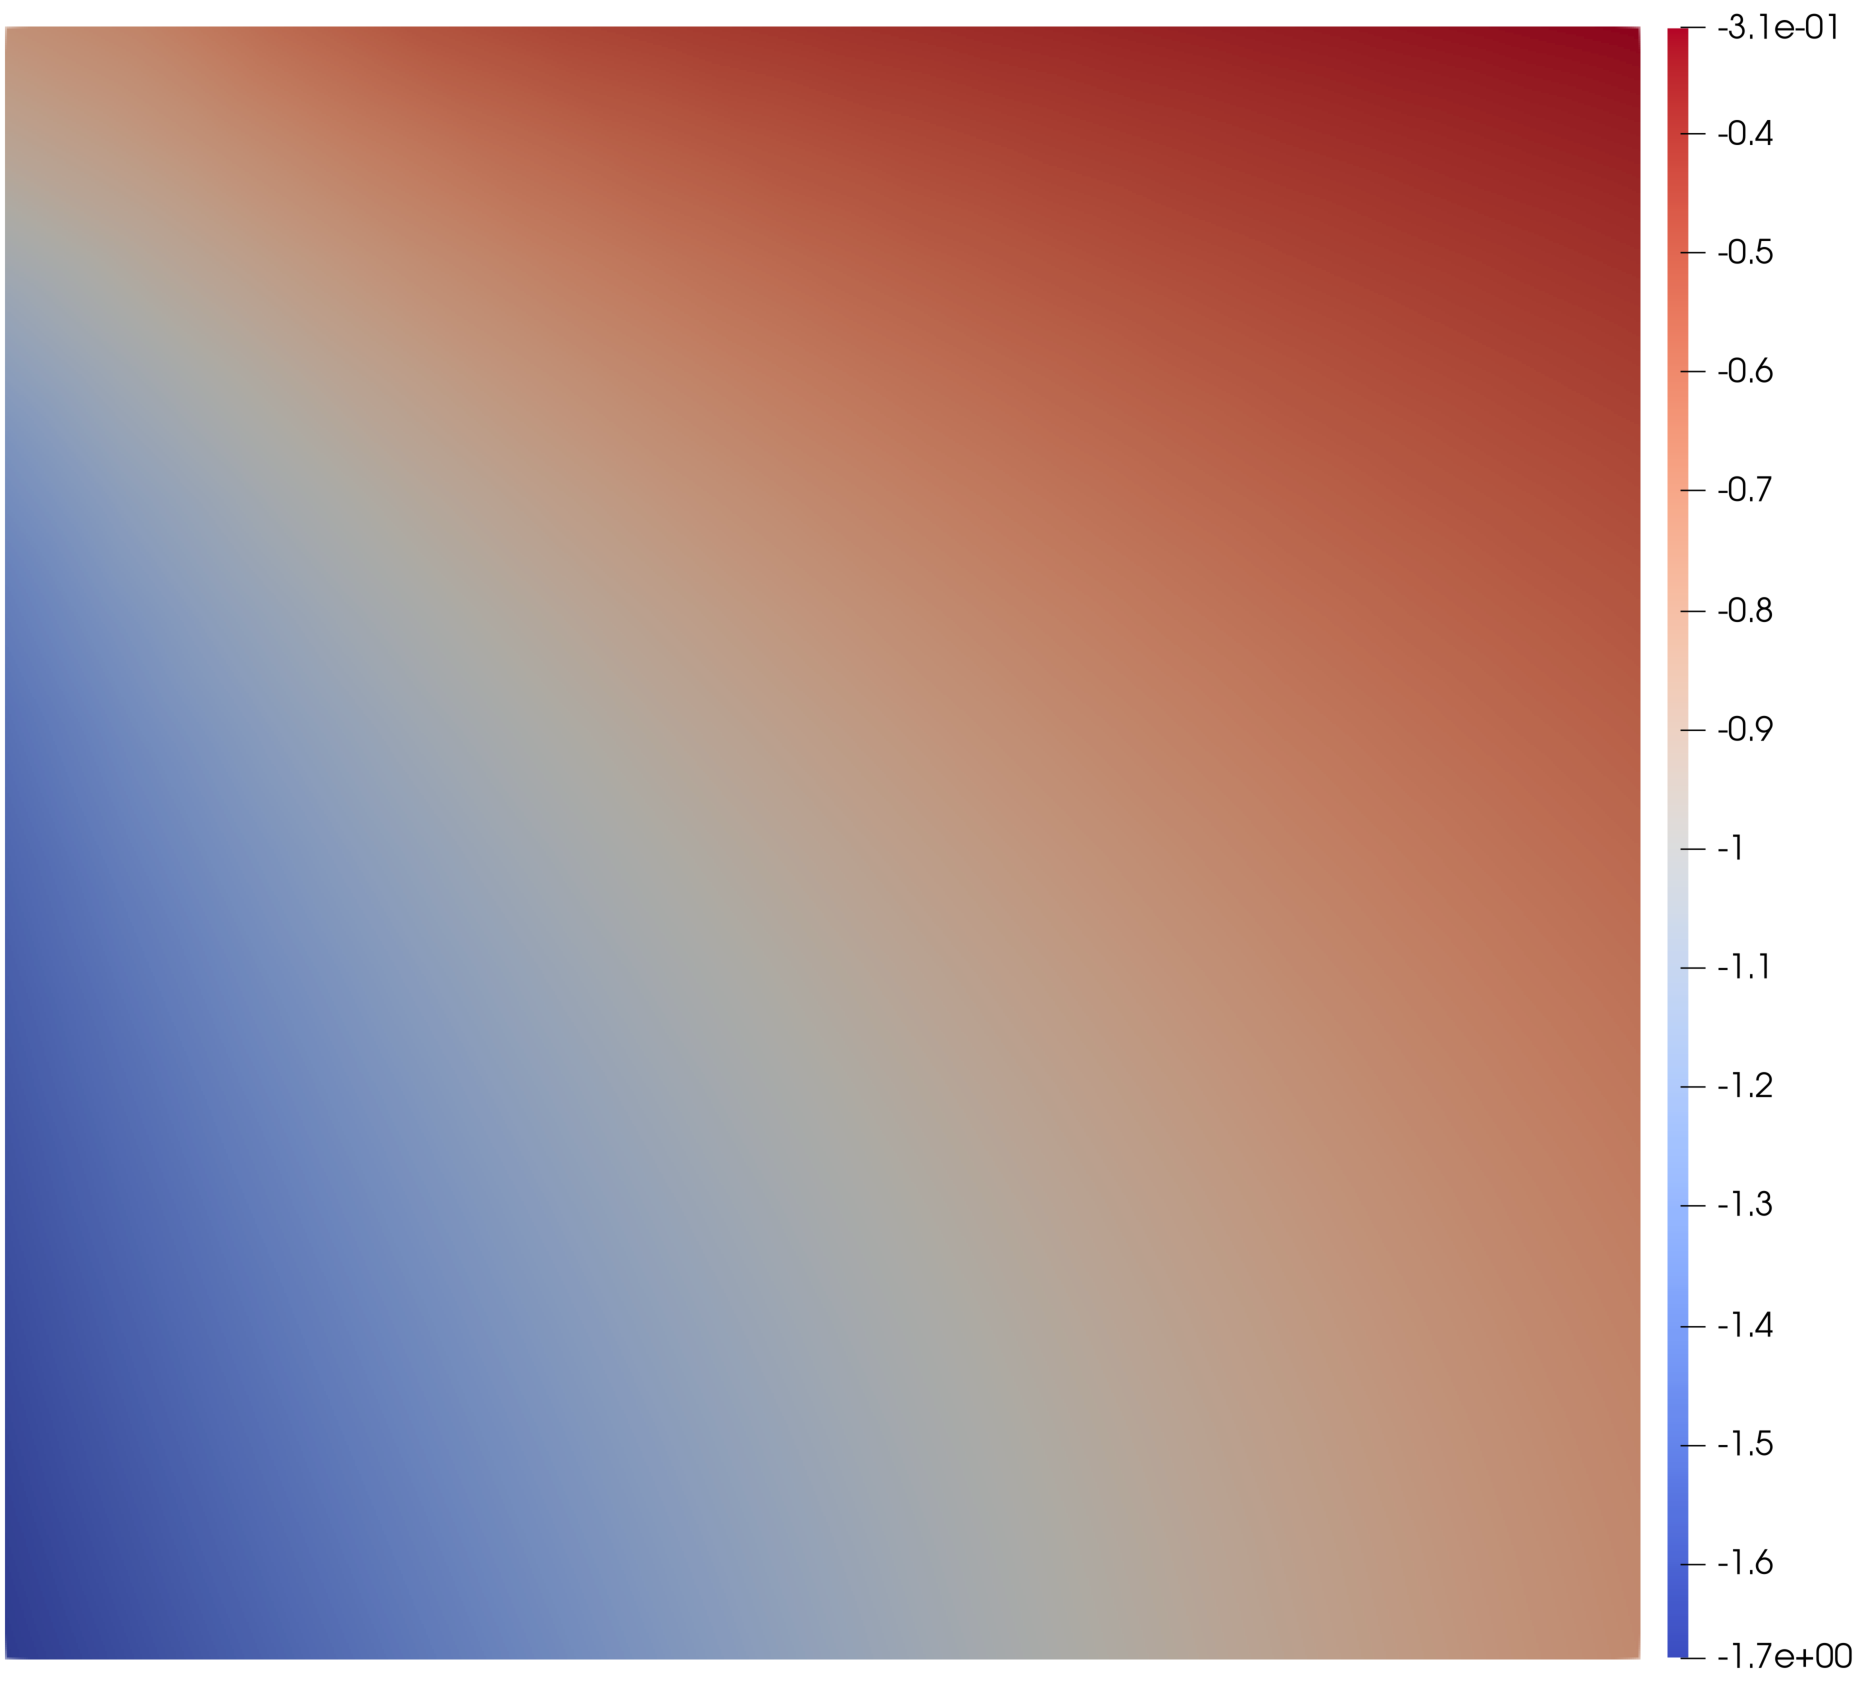
\includegraphics[scale=0.176]{images/scal_field.pdf}
  \hfill
  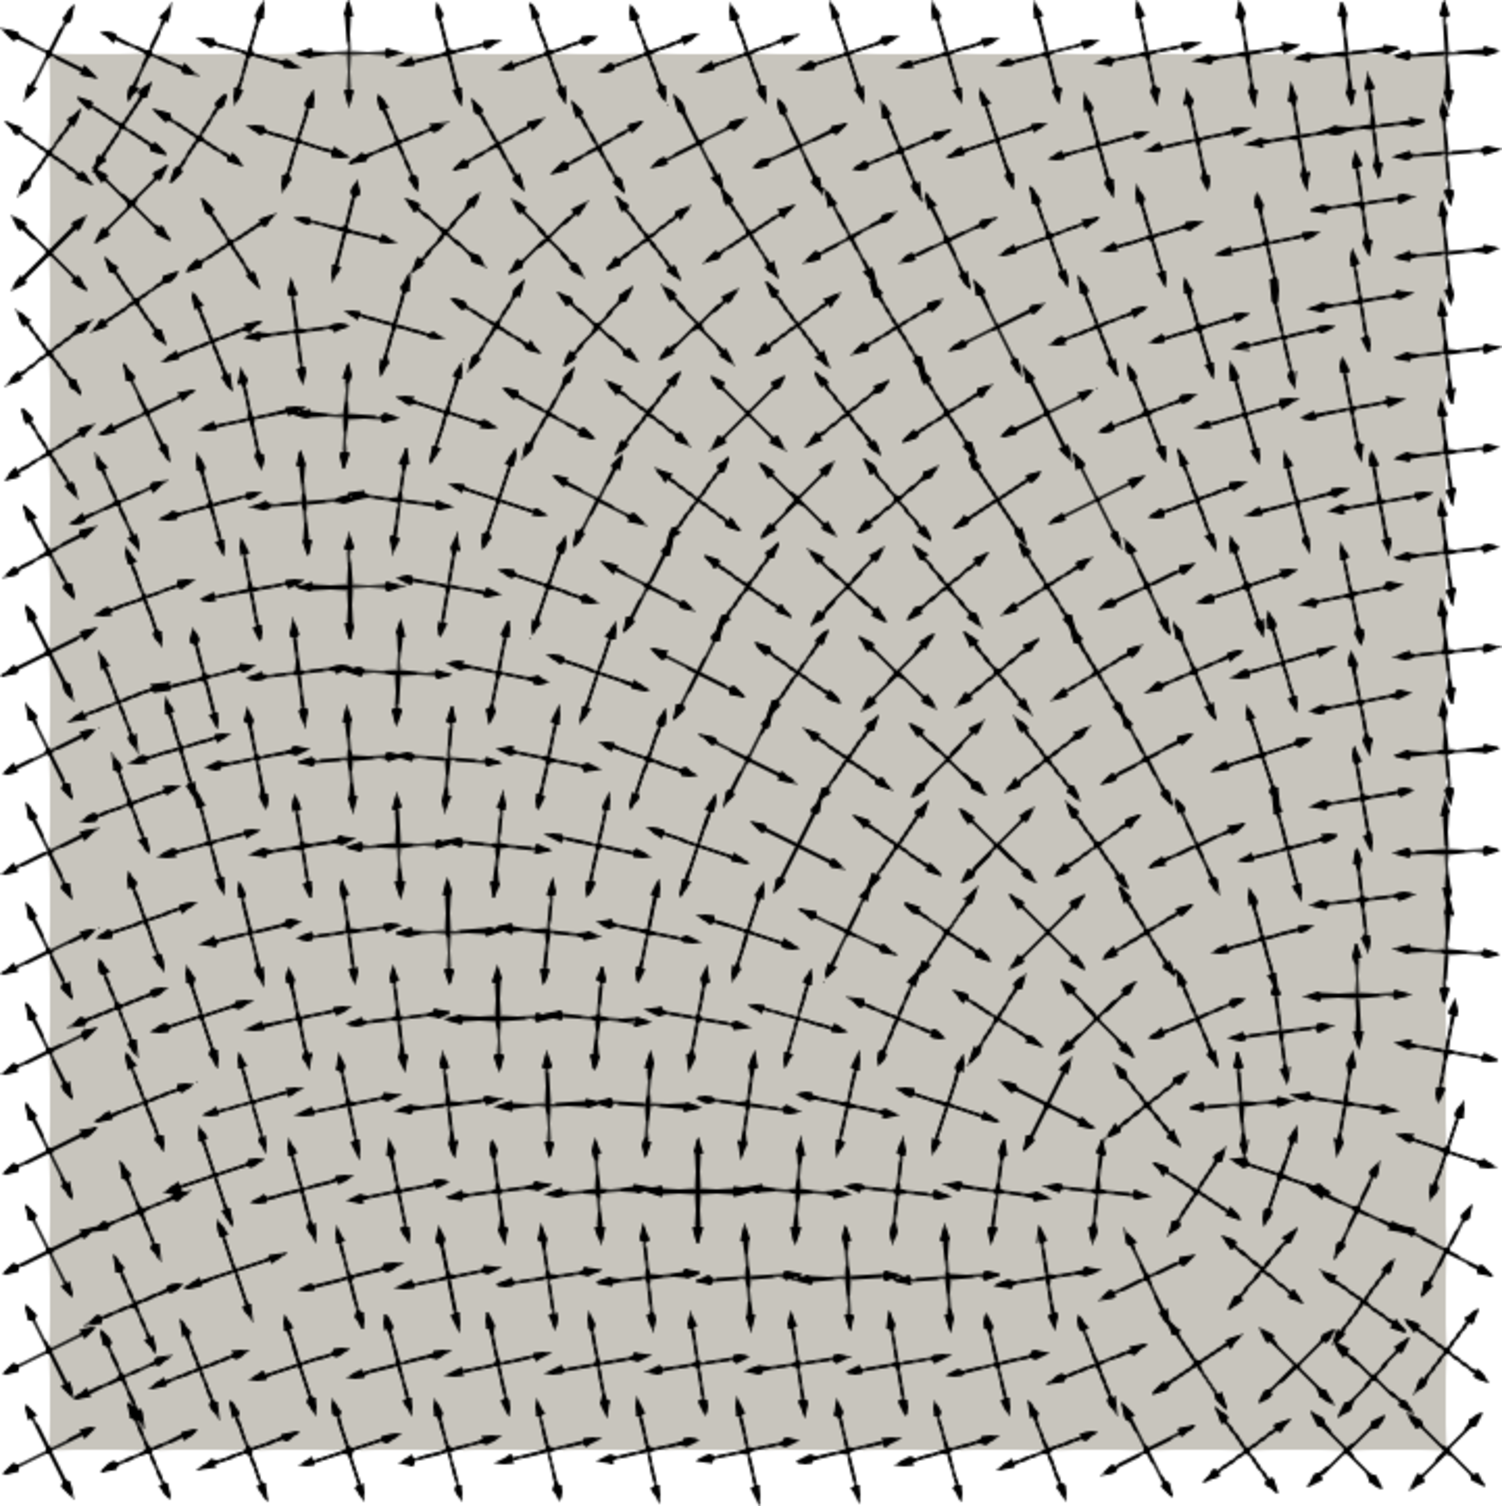
\includegraphics[scale=0.171]{images/result_field.pdf}
  \caption{Illustration de la rotation d'un champ de croix par rapport à un champ d'angle sur un domaine quelconque. \'A gauche : champ de croix initial, au milieu: champ d'angle (en radian), à droite: champ de croix résultant.}
  \label{fig:rot_cross}
\end{figure}

Pour tout point $p$ situé sur la frontière $\partial\Omega$, nous définissons $n(p)$ comme étant la normale extérieure unitaire. Lorsque la normale n'est pas définie en $p$, nous posons $n(p)=(0,0)$. En accord avec la proposition \ref{prop:cont1}, nous introduisons un champ de croix particulier associé à la frontière de $\Omega$, dite \emph{champ de croix normal} et définit par:
\begin{equation}
    \bar{n}(p) =
\left\{
    \begin{array}{ll}
        \left\{\mathbf{R}\left(\frac{m\pi}{2}\right)n(p),~ m\in \mathbb{Z}\right\} &\text{ si }n(p)\neq (0,0),\\\\
        0& \text{ sinon }.
    \end{array}
\right.
\end{equation}
Nous pouvons alors introduire la notion d'alignement du champ de croix par la définition suivante:
\begin{definition}
    Le champ de croix $\bar{u}$ est dit aligné par rapport à $\partial\Omega$ ou aligné sur le bord de $\Omega$ si pour tout point $p\in\partial\Omega$, $\bar{u}(p)\in\{\bar{n}(p), 0\}$.
\end{definition}
Nous donnons sur la figure \ref{fig:align_bord} une illustration d'un champ de croix aligné sur le bord d'un domaine.

\begin{figure}[h!]
  \centering
  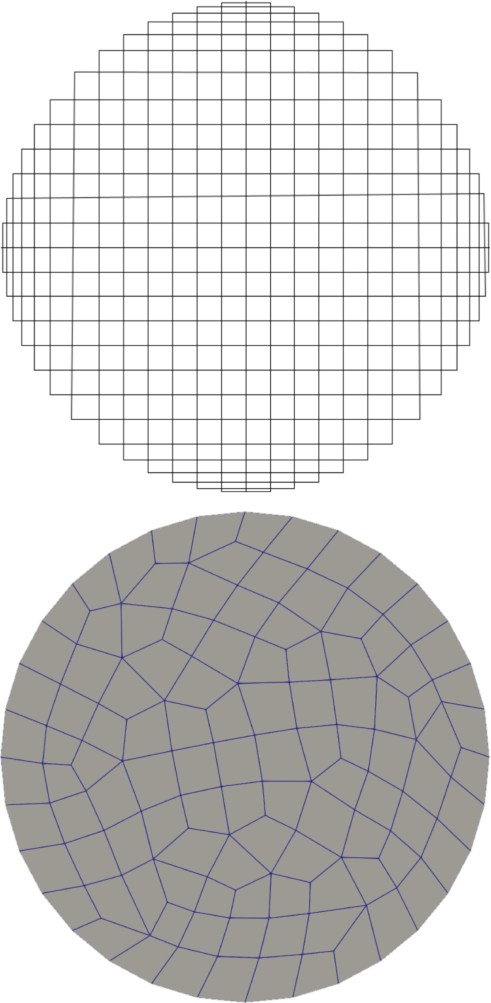
\includegraphics[scale=0.32]{images/align_bord.pdf}
  \caption{Mise en évidence d'un champ de croix aligné le long du bord d'un carré, avec une annulation du champ dans les coins.}
  \label{fig:align_bord}
\end{figure}

\subsection{Indice}

L'indice de Poincaré est un concept mathématique très usité dans la topologie et la géométrie différentielle. Il permet de quantifier le comportement des courbes et des champs de vecteurs à travers leurs singularités. Dans cette partie, à l'instar du concept d'indices pour les champs de vecteurs, nous introduisons un indice spécifique pour les champs de croix. Cet indice sera plus tard relié à la notion de \emph{séparatrices}.

Pour commencer, nous définissons la notion d'angle pour une croix. À chaque croix, nous associons une représentation angulaire. Cette approche consiste à attribuer à la croix une valeur représentant son orientation par rapport à une référence donnée.

\begin{definition}
    \label{def:cross_angle}
    Soit une croix $\mathbf{c}\in\mathbf{C}\backslash\{0\}$. L'angle associé à $\mathbf{c}$ est donné par l'unique élément de l'ensemble:
    %$$\left\{\theta_{\bar{u}}\right\} :=
    $$\{\theta_{\mathbf{c}}\} := \left\{\arg c,~c\in \mathbf{c}\right\} \cap \left]-\frac{\pi}{4},\frac{\pi}{4}\right],$$
    où $\arg c\equiv atan2(c_y, c_x)\pmod{2\pi}$ est l'argument complexe de $c=(c_x, x_y)$ pour tout $c\in\mathbf{c}$.
\end{definition}

\begin{lemma}
    L'angle donné par la définition \ref{def:cross_angle} est bien défini.
\end{lemma}

\begin{proof}
    Existence: L'ensemble $\left\{\arg c,~c\in \mathbf{c}\right\} \cap \left]-\frac{\pi}{4},\frac{\pi}{4}\right]$ est non vide. En effet, $\mathbf{c}$ étant une croix, par définition on a $\left\{\arg c,~c\in \mathbf{c}\right\} \cap \left]-\frac{\pi}{4},\frac{\pi}{4}\right]\neq\emptyset$ sauf si $\mathbf{c}=0$ ce qui est exclut.\\
    Unicité: Supposons que $\mathbf{c}$ ait deux angles $\theta_{\mathbf{c}}$ et $\theta^{'}_{\mathbf{c}}$. Par définition il existe $m, m'\in\mathbb{Z}$ et $c,c^{'}\in\mathbf{c}$ tel que:
    $$
    \theta_{\mathbf{c}}-\theta^{'}_{\mathbf{c}}=atan2(c_y, c_x)+2m\pi-atan2(c^{'}_y, c^{'}_x)-2m'\pi.
    $$
    De plus par définition il existe $l\in\mathbb{Z}$ tel que:
    $$
    atan2(c^{'}_y,c^{'}_x)=atan2(c_y,c_x)+l\frac{\pi}{2}.
    $$
    On a donc:
    $$
    \theta_{\mathbf{c}}-\theta^{'}_{\mathbf{c}}=2m\pi-2m'\pi-l\frac{\pi}{2}=k\frac{\pi}{2},
    $$
    où $k=4m-4m'-l$.
    Sachant que $\theta_{\mathbf{c}},\theta_{\mathbf{c}}^{'}\in\left]-\frac{\pi}{4},\frac{\pi}{4}\right]$, on a $\theta_{\mathbf{c}}-\theta^{'}_{\mathbf{c}}\in\left]-\frac{\pi}{2},\frac{\pi}{2}\right[$ ce qui implique que:
    $$
    -\frac{\pi}{2}<k\frac{\pi}{2}<\frac{\pi}{2}.
    $$
    Il vient donc que $k=0$ puisque $k\in\mathbb{Z}$. Autrement dit, $\theta_{\mathbf{c}}=\theta_{\mathbf{c}}^{'}$.
\end{proof}

%Comme dans \cite{beaufort2017computing}, $\Theta$ peut être vue comme l'angle minimum des vecteurs composant la croix $\mathbf{c}$.

En considérant un champ de croix $\bar{u}$, la définition précédente nous autorise donc à attribuer à $\bar{u}$ un champ scalaire formé par les angles des croix de $\bar{u}$. Ce champ est défini de la manière suivante :

\begin{definition}
    Soit $\bar{u}$ un champ de croix presque-$\mathcal{C}^1$ sur $\Omega$. Le champ d'angle associé à $\bar{u}$ est l'application définie par:
    $$\theta_{\bar{u}}:p\in\Omega\backslash\mathcal{S}_{\bar{u}}\longmapsto\theta_{\bar{u}}(p):=\theta_{\bar{u}(p)},$$
    où $\theta_{\bar{u}(p)}$ est l'angle de la croix $\bar{u}(p)$ donné par la définition \ref{def:cross_angle}.
\end{definition}

\begin{figure}[!h]
  \centering
  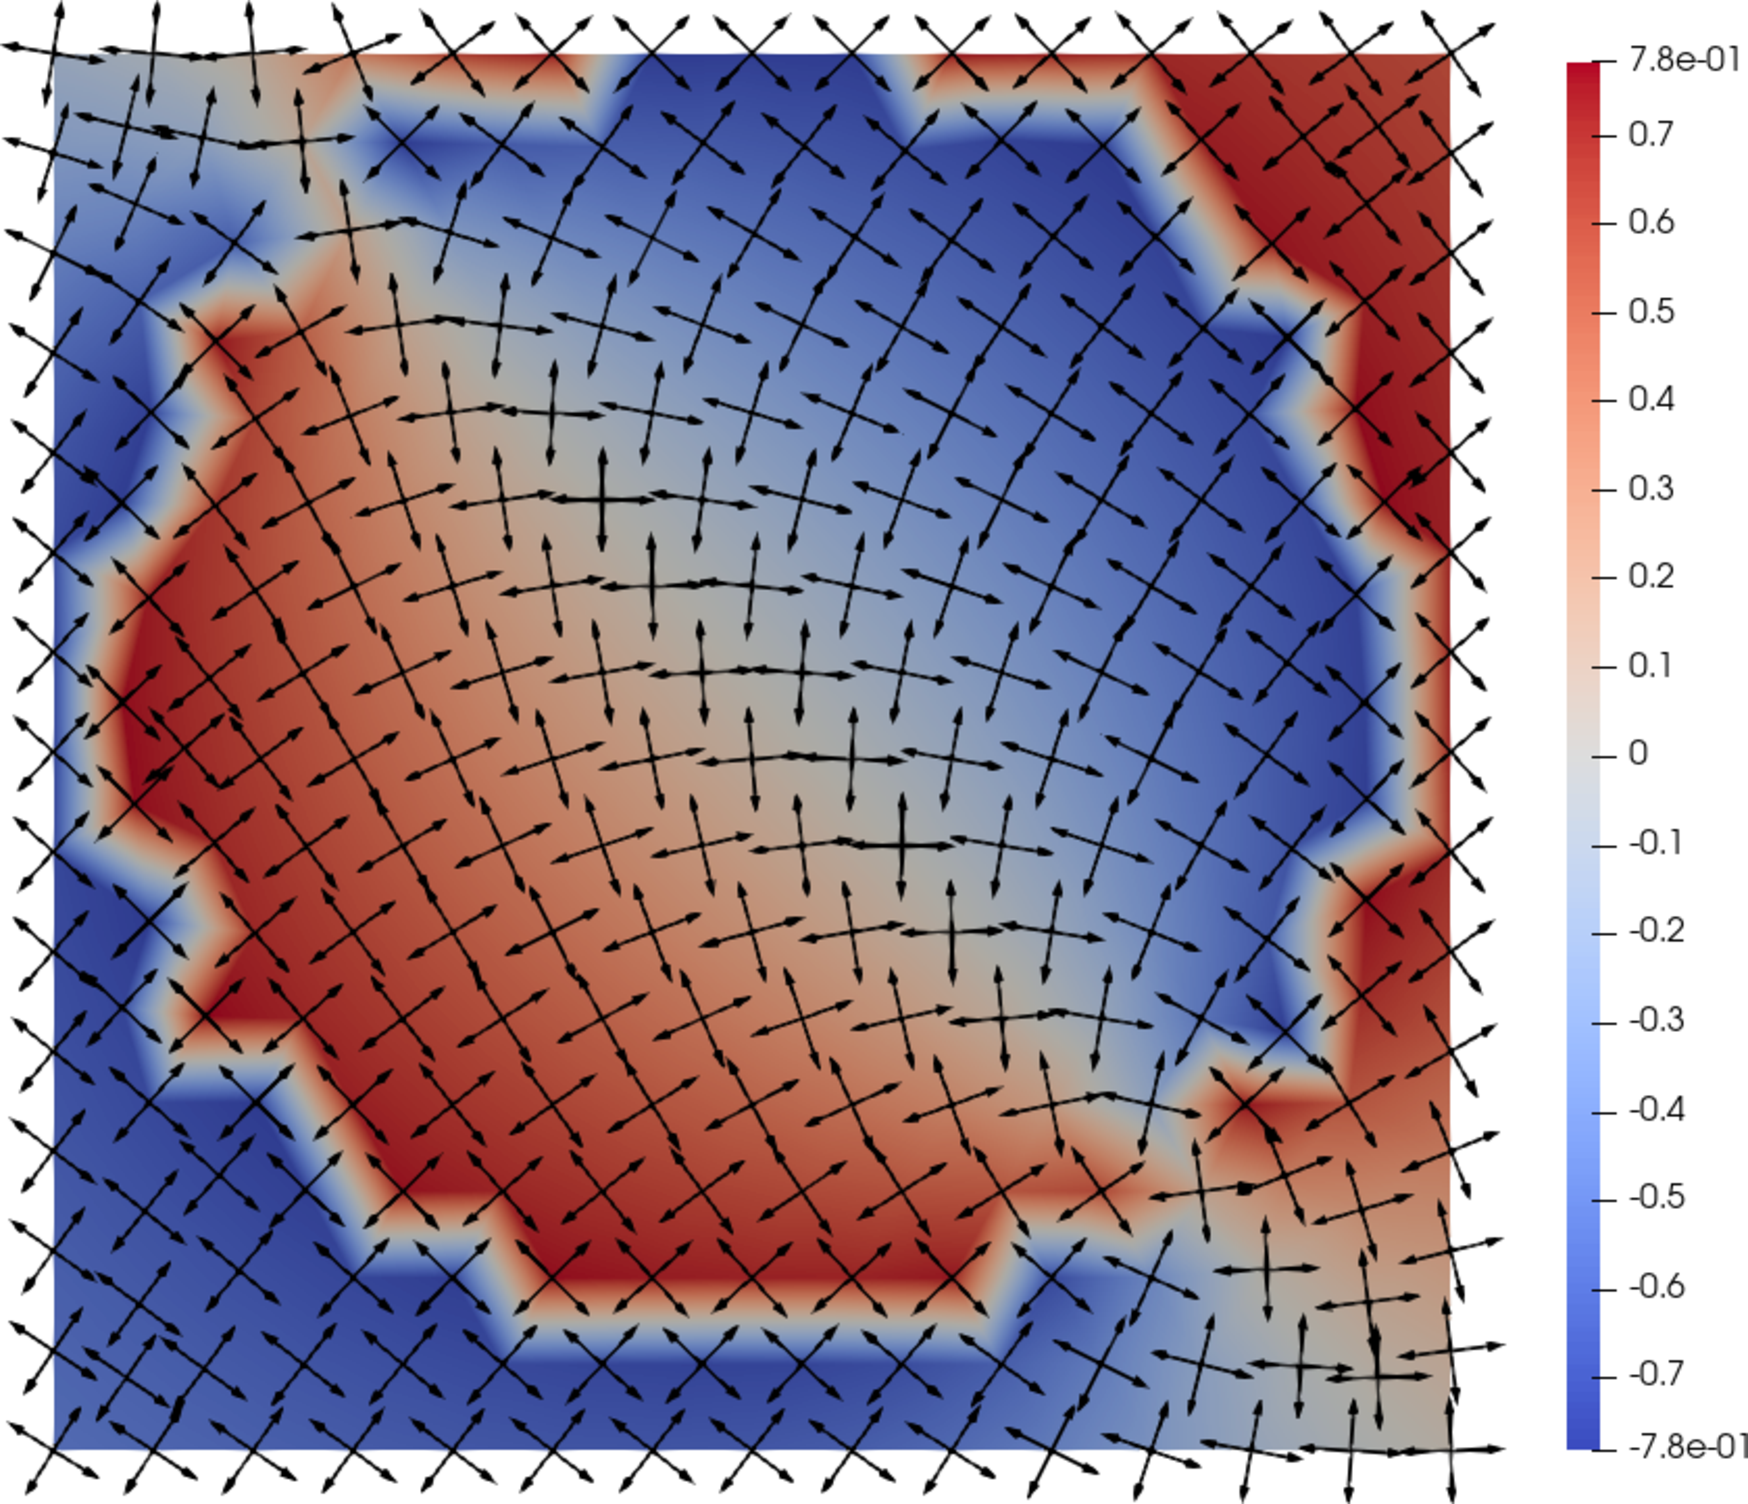
\includegraphics[scale=0.35]{images/cross_ang_field.pdf}
  \caption{Illustration d'un champ de croix et du champ d'angle (en radian) correspondant.}
  \label{fig:cross_field}
\end{figure}


Nous énonçons à présent le résultat suivant, qui constitue un outil précieux pour analyser la régularité d'un champ de croix donné à partir de la régularité du champ d'angle qui lui est associé.

\begin{proposition}
    \label{prop:angular_cont}
    Soit $\bar{u}$ un champ de croix sur $\Omega$. $\bar{u}$ est de classe $\mathcal{C}^1$ en un point $p\in\Omega$ si et seulement s'il existe $V_p\subset \Omega \backslash \mathcal{S}_{\bar{u}}$, un voisinage de $p$, et une fonction $\theta_{\bar{u}}^{V_p}:V_p \rightarrow \mathbb{R}$ telle que $\theta_{\bar{u}}^{V_p}\in \mathcal{C}^1(V_p)$ et vérifiant $\theta_{\bar{u}}^{V_p}(q)\equiv\theta_{\bar{u}}(q) \pmod{\frac{\pi}{2}}$, pour tout $q\in V_p$.
\end{proposition}


\begin{proof}
    Supposons que $\bar{u}$ est de classe $\mathcal{C}^1$ en un point $p\in\Omega$. Par définition, il existe une application $\pi_{\bar{u}}$ de classe $\mathcal{C}^1$ dans un voisinage $V_p$ de $p$. Par conséquent, la fonction $\theta_{\bar{u}}^{V_p}:=\arg \pi_{\bar{u}}$ est de classe $\mathcal{C}^1$ dans $V_p$. De plus, pour tout $q\in V_p$, $\pi_u(q)\in\bar{u}(q)$ autrement dit, pour tout $q\in V_p$, il existe $m\in\mathbb{Z}$ tel que $\arg\pi_{\bar{u}}(q)=\theta_{\bar{u}}(q)+m\frac{\pi}{2}$. On en déduit que $\theta_{\bar{u}}^{V_p}$ vérifie $\theta^{V_p}_{\bar{u}}(q)\equiv\theta_{\bar{u}}(q)\pmod{\frac{\pi}{2}}$ pour tout $q\in V_p$.

    Réciproquement, supposons qu'il existe $V_p\subset \Omega \backslash \mathcal{S}_{\bar{u}}$, un voisinage de $p$, et une fonction $\theta_{\bar{u}}^{V_p}:V_p \rightarrow \mathbb{R}$ telle que $\theta_{\bar{u}}^{V_p}\in \mathcal{C}^1(V_p)$ et vérifiant $\theta_{\bar{u}}^{V_p}(q)\equiv\theta_{\bar{u}}(q) \pmod{\frac{\pi}{2}}$, pour tout $q\in V_p$. Il vient que l'application $\pi_{\bar{u}}:=\mathbf{R}(\theta_{\bar{u}}^V)(1,0)$ est de classe $\mathcal{C}^1$ sur $V_p$. De plus, pour tout $q\in V_p$, $\pi_{\bar{u}}(q)\in \bar{u}(q)$ puisqu'il existe $m\in\mathbb{Z}$ tel que $\arg\pi_{\bar{u}}(q)=\theta_{\bar{u}}(q)+m\frac{\pi}{2}$. Ainsi $\bar{u}$ est de classe $\mathcal{C}^1$ en $p$.
\end{proof}


Grâce au résultat précédent, nous pouvons déduire le corollaire suivant permettant de construire le relèvement continu de l'angle d'un champ de croix le long d'une courbe paramétrée.

\begin{corollary}
    \label{cor:relevement_continu}
    Soit $\gamma: [0, 1] \longrightarrow \Omega$ un arc sur $\Omega$ et $\bar{u}$ un champ de croix presque-$\mathcal{C}^1$ défini sur $\Omega$ tel que pour tout $p\in\gamma([0, 1])$, $\bar{u}(p)\neq 0$. Alors, il existe $\theta^\gamma_{\bar{u}}: [0, 1] \longrightarrow \mathbb{R}$  une fonction de classe $\mathcal{C}^1$ sur $]0,1[$ telle que $\theta^\gamma_{\bar{u}}(t) \equiv \theta_{\bar{u}}(\gamma(t)) \pmod{\frac{\pi}{2}}$. De plus, si $\alpha_{\bar{u}}^\gamma$ et $\beta_{\bar{u}}^\gamma$ sont deux fonctions de classe $\mathcal{C}^1$ satisfaisant cette propriété, alors il existe $m \in \mathbb{Z}$ tel que $\alpha_{\bar{u}}^\gamma(t) = \beta_{\bar{u}}^\gamma(t) + m\frac{\pi}{2}$ pour tout $t \in [0, 1]$.
\end{corollary}

\begin{proof}
    Pour démontrer ce résultat, nous commençons par construire un recouvrement fini de $\gamma$. Nous construisons ensuite $\theta_{\bar{u}}^\gamma$ par morceaux sur les éléments du recouvrement.

    \paragraph{Construction d'un recouvrement de la courbe $\gamma$:} Soit $p\in\gamma([0, 1])$. D'après la proposition \ref{prop:angular_cont}, il existe $V_p\subset\Omega\backslash\mathcal{S}_{\bar{u}}$ et une fonction $\theta_{\bar{u}}^{V_p}\in\mathcal{C}^1$ vérifiant $\theta_{\bar{u}}^{V_p}(q)\equiv\theta_{\bar{u}}(q)\pmod{\frac{\pi}{2}}$ pour tout $q\in V_p$. Notons maintenant $\widetilde{V_p}$ la composante connexe de l'ensemble $V_p\cap\gamma([0, 1])$ et contenant $p$. Il est clair que la famille $(\widetilde{V_p})_{p\in\gamma([0, 1])}$ recouvre $\gamma([0, 1])$ puisque $\displaystyle\cup_{p\in\gamma([0, 1])}\widetilde{V_p}$ contient $\gamma([0, 1])$. $\gamma$ étant continu et $[0, 1]$ étant compact, on peut extraire de ce recouvrement, un sous-recouvrement fini de $\gamma([0, 1])$. Autrement dit, il existe $I\subset\mathbb{N}$ une partie finie de $\mathbb{N}$ et une sous-famille $(V_i)_{i\in I}$ de $(\widetilde{V_p})_{p\in\gamma([0, 1])}$ recouvrant $\gamma([0, 1])$.

    \paragraph{Construction de $\theta_{\bar{u}}^\gamma$ par morceau:} Soit $\{p_0\}=\gamma^{-1}(0)$ et $V_0\in(V_i)_{i\in I}$ tel que $p_0\in V_0$. On définit $\theta_{\bar{u}}^\gamma(t):=\theta_{\bar{u}}^{V_0}\circ\gamma(t)$ pour tout $t\in\gamma^{-1}(V_0\cap\gamma([0, 1]))$. Il est clair que $\theta_{\bar{u}}^\gamma\in\mathcal{C}^1(\gamma^{-1}(V_0\cap\gamma(]0, 1[))$ et $\theta_{\bar{u}}^\gamma(t)\equiv\theta_{\bar{u}}(\gamma(t))\pmod{\frac{\pi}{2}}$ pour tout $t\in\gamma^{-1}(V_0\cap\gamma([0, 1]))$. À partir de là, nous itérons la construction de $\theta^\gamma_{\bar{u}}$ de la manière suivante: pour $n>0$, on choisit le point $p_n$ tel que $p_n\in\partial V_{n-1}\cap\gamma([0, 1])$ et $p_n\notin\{p_0,\dots,p_{n-1}\}$. On choisit ensuite $V_n$ tel que $V_n\in(V_i)_{i\in I}$, $V_n\neq V_k,~k<n$ et $p_n\in V_n$. D'après la proposition \ref{prop:angular_cont}, il existe $\theta_{\bar{u}}^{V_n}\in\mathcal{C}^1(V_n)$ et pour tout $q\in V_n$, $\theta_{\bar{u}}^{V_n}(q)\equiv\theta_{\bar{u}}(q)\pmod{\frac{\pi}{2}}$. Soit $m\in\mathbb{Z}$ tel que $\theta^{V_n}_{\bar{u}}\circ\gamma(t)+m\frac{\pi}{2}=\theta^\gamma_{\bar{u}}(t)$ pour tout $t\in\gamma^{-1}(V_{n-1}\cap\gamma([0, 1]))\cap\gamma^{-1}(V_n\cap\gamma([0, 1]))$. On définit alors $\theta_{\bar{u}}^\gamma(t):=\theta^{V_n}_{\bar{u}}\circ\gamma(t)+m\frac{\pi}{2}$ pour tout $t\in\gamma^{-1}(V_n\cap\gamma([0, 1)])$. Il est clair que $\theta_{\bar{u}}^\gamma$ ainsi définit est de classe $\mathcal{C}^1$ sur $\cup_{k=0}^n\gamma^{-1}(V_k\cap\gamma(]0, 1[))$ et $\theta_{\bar{u}}^\gamma(t)\equiv\theta_{\bar{u}}\circ\gamma(t)\pmod{\frac{\pi}{2}}$ pour tout $t\in\cup_{k=0}^n\gamma^{-1}(V_k\cap\gamma([0, 1]))$. On poursuit itérativement cette construction jusqu'à ce que $\cup_{k=0}^n\gamma^{-1}(V_k\cap\gamma([0, 1]))=\gamma([0, 1])$. Le nombre d'itération à faire est fini puisque $(V_i)_{i\in I}$ est un recouvrement fini de $\gamma([0, 1])$.
    \[\]
    Supposons maintenant que $\alpha_{\bar{u}}^\gamma$ et $\beta_{\bar{u}}^\gamma$ soient deux fonctions de classe $\mathcal{C}^1$ qui satisfont cette propriété, alors, il existe des fonctions $g:[0, 1]\longrightarrow\mathbb{Z}$ et $h:[0, 1]\longrightarrow\mathbb{Z}$ telles que $\alpha^\gamma_{\bar{u}}(t) = \theta_{\bar{u}}(\gamma(t)) + g(t)\frac{\pi}{2}$ et $\beta^\gamma_{\bar{u}}(t) =\theta_{\bar{u}}(\gamma(t)) + h(t)\frac{\pi}{2}$. Par conséquent, pour tout $t\in[0, 1]$ on a:
    $$\alpha_{\bar{u}}^\gamma(t) = \beta_{\bar{u}}^\gamma(t) + g(t)\frac{\pi}{2}-h(t)\frac{\pi}{2}.$$
    $\alpha^\gamma_{\bar{u}}$ et $\beta^\gamma_{\bar{u}}$ étant continue sur $[0, 1]$, il vient que la fonction $g-h$ est continue sur $[0, 1]$. Autrement dit, $g-h$ est constant car continue et à valeur dans $\mathbb{Z}$. Soit $m\in\mathbb{Z}$ tel que $m=(g-h)(t)$, pour tout $t\in[0, 1]$, On a:
    $$\forall t\in[0, 1],\quad\alpha_{\bar{u}}^\gamma(t) = \beta_{\bar{u}}^\gamma(t) + m\frac{\pi}{2}.$$
\end{proof}

Le relèvement continu du champ de croix le long d'une courbe paramétrée permet de quantifier le nombre de fois que le champ tourne sur lui-même le long de la courbe. Cependant, la construction du Corollaire \ref{cor:relevement_continu} ne fonctionne pas si $\mathcal{S}_{\bar{u}}\cap\gamma([0,1])\neq\emptyset$. Dans ce cas, nous construisons le relèvement par morceaux le long de $\gamma$ de la manière suivante :

Soit $I:=\gamma^{-1}(\mathcal{S}_{\bar{u}}\cap\gamma([0, 1]))\cup\{0, 1\}$. On a $Card(I)<\infty$ puisque $Card(\mathcal{S}_{\bar{u}})<\infty$. Il existe donc $(t_i)_{i\in\llbracket 1, n_I\rrbracket}\subset[0,1]$ tel que $I=(t_i)_{i\in\llbracket 1, n_I\rrbracket}$ avec $0=t_1<\dots<t_{n_I}=1$ et $n_I=Card(I)$. Par construction, il est clair que pour tout $i\in\llbracket 1, n_I-1 \rrbracket$, on a $\mathcal{S}_{\bar{u}}\cap\gamma(]t_i, t_{i+1}[)=\emptyset$. Ainsi, à partir du Corollaire \ref{cor:relevement_continu}, nous pouvons construire pour tout $i\in\llbracket 1, n_I-1\rrbracket$ une fonction $\theta^{\gamma_i}_{\bar{u}}$ sur $[0,1]$ et de classe $\mathcal{C}^1$ sur $]0,1[$ telle que $\theta_{\bar{u}}^{\gamma_i}(t)\equiv\theta_{\bar{u}}(\gamma_i(t))\pmod{\frac{\pi}{2}}$ avec $\gamma_i$, l'arc défini sur $[0, 1]$ par :
$$
\forall t\in[0, 1],~\gamma_i(t)=\gamma(t_i+t(t_{i+1}-t_i)).
$$
Finalement, le relèvement $\theta_{\bar{u}}^\gamma$ le long de $\gamma$ est donné par:
\begin{eqnarray*}
    \forall i\in\llbracket 1, n_I\rrbracket,~\forall t\in]t_i, t_{i+1}[,~\theta_{\bar{u}}^\gamma(t)=\theta_{\bar{u}}^{\gamma_i}\left(\frac{t-t_i}{t_{i+1}-t_i}\right).
\end{eqnarray*}



Grâce à cette notion, nous sommes désormais en mesure de définir l'indice d'un point dans un champ de croix.



\begin{comment}
    \begin{figure}[!h]
  \centering
  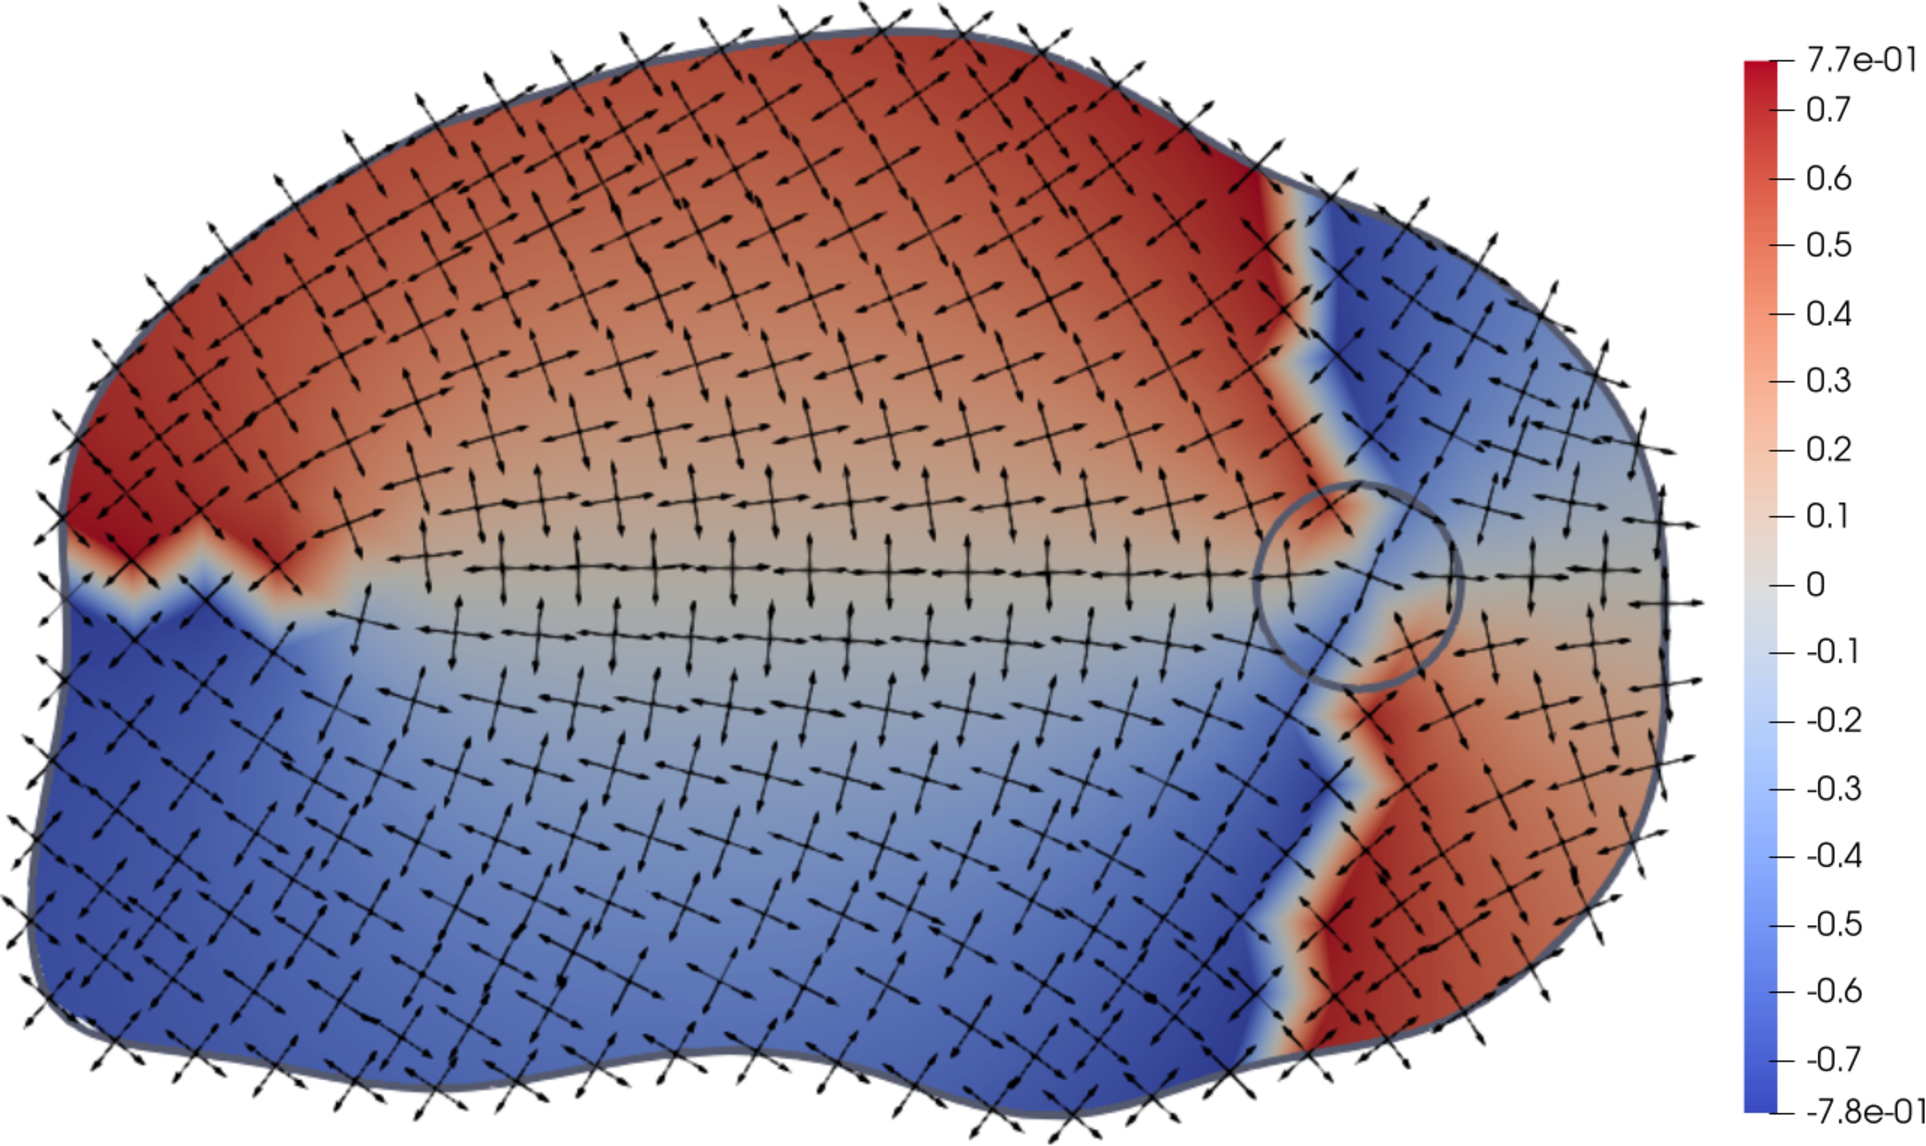
\includegraphics[scale=0.25]{images/lifting_cross_ang.pdf}\hspace{0.5cm}
  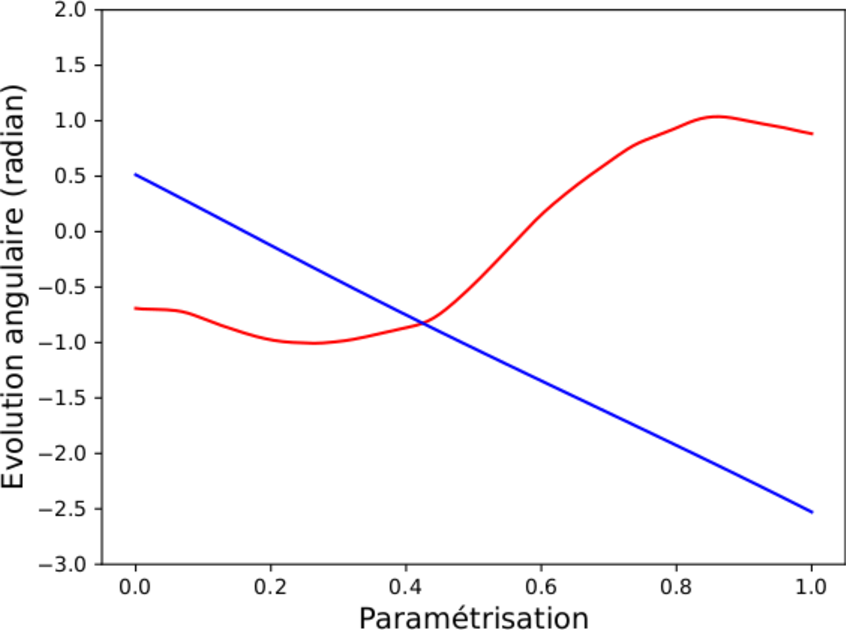
\includegraphics[scale=0.45]{images/lifting_courbe.pdf}
  \caption{Illustration du relèvement continu d'un champ de croix (à gauche avec son champ d'angle associé en radian) le long de courbes paramétriques. En bleu: la courbe paramétrique intérieur, en rouge la courbe paramétrique représentant le bord du domaine.}
  \label{fig:lifting}
\end{figure}
\end{comment}

\begin{definition}
    On appelle chemin fermé tout lacet $\Gamma$ qui est $\mathcal{C}^0\cap\mathcal{C}^1_m$. On appellera paramétrisation simple de $\Gamma$, toute paramétrisation $\gamma : I\subset\mathbb{R}\longrightarrow\Gamma$ telle que l’ensemble $\{s\in I, \exists t\in I,~s\neq t,~ \gamma(s) = \gamma(t)\}$ est d’intérieur vide dans $\mathbb{R}$.
\end{definition}

Dans tout ce qui suit, les paramétrisations des lacets seront supposées être des paramétrisations simple et on aura par définition l'intégrale sur $\Gamma$ d'une fonction notée $f$ par rapport au lacet $\gamma$ de $\Gamma$
$$
\int_\gamma f:=\int_If(\gamma(s))\gamma'(s)ds,
$$
indépendante de $\gamma$. On notera $V^\Gamma$ une partie de $\Omega$ délimitée par $\Gamma$. Soit $\overrightarrow{n}(q)$ la normale extérieur en $q$ à $V^\Gamma$. On dit que $\gamma$ paramétrise $\Gamma$ dans le sens positif si pour tout $t\in I$, $(\gamma'(t)\wedge\overrightarrow{n}(\gamma(t))).(0,0,1)^t>0$ Dans la suite, nous adoptons la notation suivante:

$$
\int_\Gamma d\theta_{\bar{u}}:=\int_\gamma d\theta_{\bar{u}}:=\int_a^b d\theta_{\bar{u}}^\gamma.
$$

\begin{lemma}
    \label{lem:index_saga_first}
    Soit $\bar{u}$ un champ de croix presque-$\mathcal{C}^1$ et $\Gamma$ un chemin fermé dont $\gamma$ est une paramétrisation sur $[a,b]$. La fonction $F(\Gamma)$ suivante
    $$
    F_{\bar{u}}(\Gamma):=\frac{1}{2\pi}\int_a^b d\theta_{\bar{u}}^\gamma,
    $$
    vérifie $4F_{\bar{u}}(\Gamma)\in\mathbb{Z}$. En outre, si $(V^{\Gamma_i})_{i\in\llbracket 1, n_\Gamma\rrbracket}$ forme une partition de $V^\Gamma$ telle que $\bar{u}(p)\neq 0,~\forall p\in\Gamma_i,~\forall i\in\llbracket 1, n_\Gamma\rrbracket$, alors on a:
    \begin{equation}
        F_{\bar{u}}(\Gamma)=\sum_{i=1}^{n_\Gamma}F_{\bar{u}}(\Gamma_i).
        \label{eqn:sum_F_u}
    \end{equation}
\end{lemma}

\begin{proof}
    Soit $w(p)-z=e^{4i\theta_{\bar{u}}^\gamma(p)}$ si $\bar{u}(p)\neq 0$ et $w(p)-z=0$ sinon, avec $z\in\mathbb{C}$ alors on a (comme dans \cite{rudin1998analyse}):
    $$
    \int_\gamma\frac{dw}{w-z}=\int_\gamma d \ln(w-z)=\int_\gamma 4id\theta_{\bar{u}}^\gamma.
    $$
    Il vient donc que:
    $$
    2\pi F_{\bar{u}}(\Gamma)=\frac{1}{4}Im\left(\int_\gamma\frac{dw}{w-z}\right).
    $$
    Montrer que $4F_{\bar{u}}(\Gamma)\in\mathbb{Z}$ revient alors à montrer que:
    $$
    exp\left(\int_a^b\frac{w'(\gamma(t))\gamma'(t)}{w(\gamma(t))-z}dt\right)=1,
    $$
    si $w\circ\gamma(t)\neq z$ hormis un sous-ensemble discret de valeurs $t\in[a, b]$ (ce qui est le cas pour $z = 0$ avec $\bar{u}$ n’ayant que des zéros isolés).\\
    Posons
    $$
    \varphi(t):=exp\left(\int_a^t\frac{w'(\gamma(t))\gamma'(t)}{w(\gamma(t))-z}dt\right),~t\in[a,b],
    $$
    $\varphi$ est de classe $\mathcal{C}^1$ par morceau et vérifie:
    $$
    \frac{\varphi'}{\varphi}=\frac{\gamma'.w'\circ\gamma}{w'\circ\gamma-z},
    $$
    Il vient alors que la fonction $\varphi/(w\circ\gamma-z)$ est continue, dérivable presque partout ($w\in\mathcal{C}^1$ et $\gamma\in\mathcal{C}^0\cap\mathcal{C}^1_m$) de dérivée nulle donc elle est constante (presque partout, donc partout car continue) et comme $\varphi(a)=1$, on a:
    $$
    \varphi(t)=\frac{w(\gamma(t))-z}{w(\gamma(a))-z},
    $$
    En utilisant maintenant le fait que $\gamma(a)=\gamma(b)$, il vient que $\varphi(b)=1$ et donc finalement
    $$
    \exists k\in\mathbb{Z},~\int_a^b\frac{w'(\gamma(t))\gamma't)}{w(\gamma(t))-z}dt=2ik\pi.
    $$
    Ainsi $4F_{\bar{u}}(\Gamma)\in\mathbb{Z}$.\\\\
    Pour la propriété d'additivité de $F_{\bar{u}}$ on commence par décomposer les frontières de chaque $V^{\Gamma_i}$ de la manière suivante: $\Gamma_{i,0}=\Gamma_i\cap\Gamma$ et $\Gamma_{i,j}=\Gamma_i\cap\Gamma_j$ pour $j\neq i$. Par convention on pose $\Gamma_{i,i}=\emptyset$, $\forall i\in\llbracket 1, n_\Gamma\rrbracket$. On a alors $\Gamma_i=\cup_{j\in\llbracket1, n_\Gamma\rrbracket}\Gamma_{i,j}$ et $\Gamma_{i,j}=\Gamma_{j,i}$ et on peut écrire:
    $$
    \sum_{i=1}^{n_\Gamma}F_{\bar{u}}(\Gamma_i)=\frac{1}{2\pi}\sum_{i=1}^{n_\Gamma}\sum_{j=0}^{n_\Gamma}\int_{\Gamma_{i,j}}d\theta_{\bar{u}}^\gamma=\frac{1}{2\pi}\sum_{i=1}^{n_\Gamma}\int_{\Gamma\cap\Gamma_i}d\theta_{\bar{u}}+\frac{1}{2\pi}\sum_{i=1}^{n_\Gamma}\sum_{j=1}^{n_\Gamma}\int_{\Gamma_{i,j}}d\theta_{\bar{u}}.
    $$
    Autrement dit,
    $$
    \sum_{i=1}^{n_\Gamma}F_{\bar{u}}(\Gamma_i)=F_{\bar{u}}(\Gamma)+\frac{1}{2\pi}\sum_{i=1}^{n_\Gamma}\int_{\Gamma_{i,i}}d\theta_{\bar{u}}+\frac{1}{2\pi}\sum_{1\leq i<j\leq n_\Gamma}\int_{\Gamma_{i,j}\cup\Gamma_{j,i}}d\theta_{\bar{u}}.
    $$
    Dans l'équation précédente, le second terme s'annule car $\Gamma_{i,i}=\emptyset$ et le dernier terme vaut lui aussi zéro car $\Gamma_{i,j}\cup\Gamma_{j,i}$ représente un lacet et par hypothèse $\bar{u}$ est $\mathcal{C}^1$ sur $\Gamma_i\cap\Gamma_j$. D'où le résultat.
\end{proof}

\begin{lemma}
    \label{lem:index_saga_second}
    Sous les hypothèses du lemme \ref{lem:index_saga_first}, si $\bar{u}$ est $\mathcal{C}^1$ sur un ensemble convexe $V\subset\Omega$ alors pour tout arc $\Gamma$
    %de longueur assez petite
    telle que $V^\Gamma\subset V$ on a $F_{\bar{u}}(\Gamma)=0$.
\end{lemma}

\begin{proof}
    Il suffit de remarquer que si $u$ est de classe $\mathcal{C}^1$ sur $V^\Gamma$ alors $w'$ est bornée par une constante $M>0$ sur $V^\Gamma$ et donc on a:
    $$
    \left|\int_a^b\frac{w'(\gamma(t))\gamma't)}{u(\gamma(t))-z}dt\right|\leq M\int_a^b|\gamma'(t)|dt<2\pi,
    $$
    pour $\Gamma$ décrivant un arc de longueur inférieure à $2\pi/M$, tel que $V^\Gamma\subset V$ et donc $F_u(\Gamma)=0$. On généralise ensuite ce résultat à un arc $\Gamma$ de taille quelconque en pavant $V^\Gamma$ avec des boules de rayon plus petit que $1/4\pi$ puis on conclut en utilisant le lemme \ref{lem:index_saga_first}.
\end{proof}

\begin{lemma}
    \label{lem:index_saga_third}
    Pour tout voisinnage $V^\Gamma$ de $p$ tel que $u\in\mathcal{C}^1(V^\Gamma\backslash\{p\})$, on a pour tous chemins fermés $\Gamma_1$ et $\Gamma_2$ on a:
    $$
    p\in V^{\Gamma_i}\subset V^\Gamma, \forall i=1, 2\Longrightarrow F_{\bar{u}}(\Gamma_1)=F_{\bar{u}}(\Gamma_2).
    $$
\end{lemma}

\begin{proof}
    Soient $\Gamma_1$ et $\Gamma_2$ deux lacets vérifiant les hypothèses du lemme. En notant $V_3=V^{\Gamma_1}\cap V^{\Gamma_2}$ et $\Gamma_3=\partial V^{\Gamma_3}$ qui est $\mathcal{C}^0\cap\mathcal{C}^1_m$ et $(V^i_j)_{j\in\llbracket 1, k_i\rrbracket}$ les composantes connexes de $V^{\Gamma_i}\backslash V^3$, pour $i=1,2$. En notant $\Gamma_i^j=\partial V^i_j$, qui est donc $\mathcal{C}^0\cap\mathcal{C}^1_m$. En appliquant \eqref{eqn:sum_F_u}, on obtient:
    $$
    \forall i=1,2,~F_{\bar{u}}(\Gamma_i)=\sum_{j=1,\dots,k_i}F_{\bar{u}}(\Gamma_i^j)=F_{\bar{u}}(\Gamma_3),
    $$
    par le lemme \ref{lem:index_saga_second} car $u$ est $\mathcal{C}^1$ sur chaque $V^i_j\subset V^\Gamma\backslash\{p\}$. D'où le résultat.
\end{proof}

En combinant les lemmes \ref{lem:index_saga_first} et \ref{lem:index_saga_second}, on obtient alors:

\begin{definition}
    Pour un champ $u$ n'ayant que des irrégularités isolées, on appelle indice du point p dans le champ $u$ la valeur:
    $$
    id_{\bar{u}}(p):=F_{\bar{u}}(\Gamma),
    $$
    où $\Gamma$ est un chemin fermé paramétré dans le sens positif tel que $p\in V^\Gamma$ et $u\in\mathcal{C}^1(V^\Gamma\backslash\{p\})$.
    \label{def:index}
\end{definition}

\begin{proposition}
    La définition \ref{def:index} est bien posée.
\end{proposition}

\begin{proof}
    Il s'agit d'une conséquence directe du lemme \ref{lem:index_saga_third}.
\end{proof}

On peut alors retrouver les propriétés principales de l'indice, résumées dans le théorème suivant:

\begin{theorem}
    \label{thm:index}
    L'indice du point $p$ dans le champ $u$ vérifie les propriétés suivantes:
    \begin{enumerate}
        \item $id_{\bar{u}}^\gamma(p)=k/4$, $k\in\mathbb{Z}$,
        \item si $u$ est $\mathcal{C}^1$ en $p$ alors $id_{\bar{u}}(p)=0$,
        \item pour tout chemin fermé $\Gamma$ tel que $p\in V^\Gamma$ et que $\bar{u}\in\mathcal{C}^1(V^\Gamma\backslash\{p\})$, $id_{\bar{u}}^\gamma(p)=F_{\bar{u}}(\Gamma)$.
    \end{enumerate}
\end{theorem}

\begin{proof}
    Ces résultats sont respectivement des conséquences directes des lemmes \ref{lem:index_saga_first}, \ref{lem:index_saga_second} et \ref{lem:index_saga_third}.
\end{proof}

Par extension, en utilisant le lemme \ref{lem:index_saga_first} on a:

\begin{corollary}
    \label{cor:sum_index}
Soit $V^\Gamma$ une partie de $\Omega$ délimitée par $\Gamma$. On a:
\begin{equation}
\label{eqn:Fu_sum}
 F_{\bar{u}}(\Gamma)=\sum_{p\in V^\Gamma\cap\mathcal{S}_{\bar{u}}} id_{\bar{u}}(p).
\end{equation}
\end{corollary}

\begin{proof}
Il suffit de recouvrir $V^\Gamma$ en utilisant des boules qui isolent tous les points $p\in V^\Gamma\cap\mathcal{S}_{\bar{u}}$. On applique ensuite le théorème \ref{thm:index} à chaque boule puis l'équation \eqref{eqn:Fu_sum} est obtenue en utilisant le lemme \ref{lem:index_saga_first}.
\end{proof}


\begin{comment}
    \begin{definition}[Indice]
    \label{def:index}
    Soit $\bar{u}$ un champ de croix presque-$\mathcal{C}^1$ définit sur $\Omega$ et un point $p$ dans $\Omega\backslash\partial\Omega$. L'indice de $p$ dans le champ de croix $\bar{u}$ est donné par la quantité:
    \begin{equation}
    id_{\bar{u}}(p) =\frac{1}{2\pi}\int_0^1d\theta_{\bar{u}}^\gamma,
    \label{eqn:Indexinterior}
    \end{equation}
    où $\gamma :[0 ; 1]\longrightarrow \Omega$ est un lacet entourant $p$, n'englobant aucun autre point singulier de $\bar{u}$ et paramétrisé dans le sens anti-horaire.
    \end{definition}
\end{comment}

De manière intuitive, l'indice d'un point dans un champ exprime combien de fois le champ semble s'enrouler autour de lui-même près de ce point (voir la figure \ref{fig:index_illustration}).

\begin{figure}[!h]
  \centering
  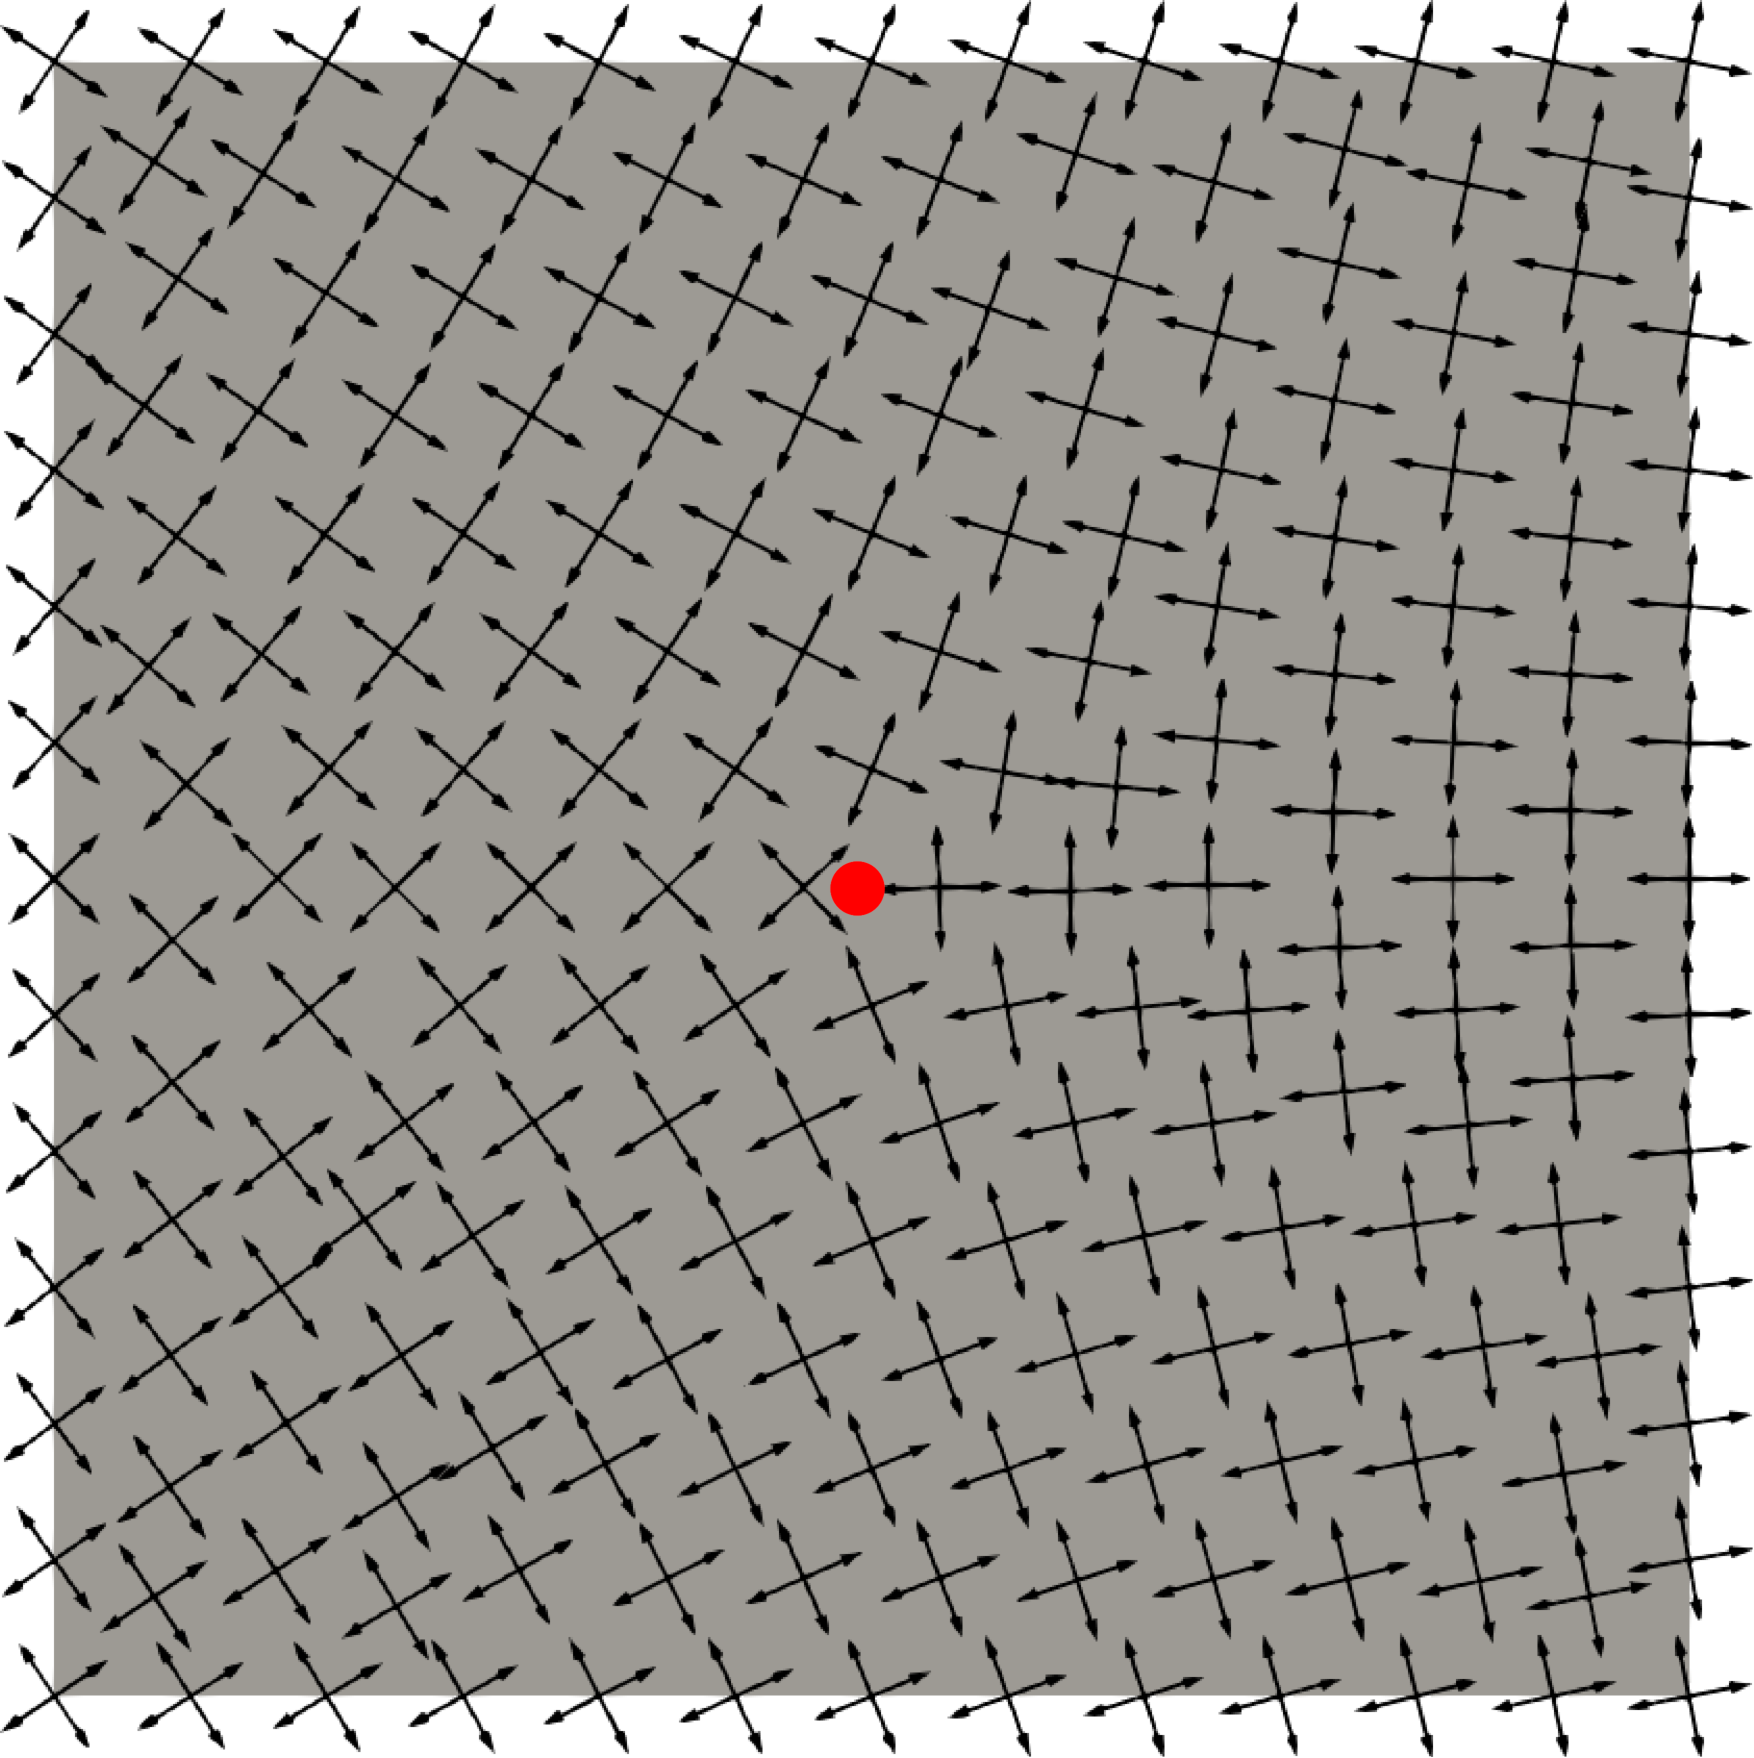
\includegraphics[scale=0.1765]{images/index_-025.pdf}
  \hfill
  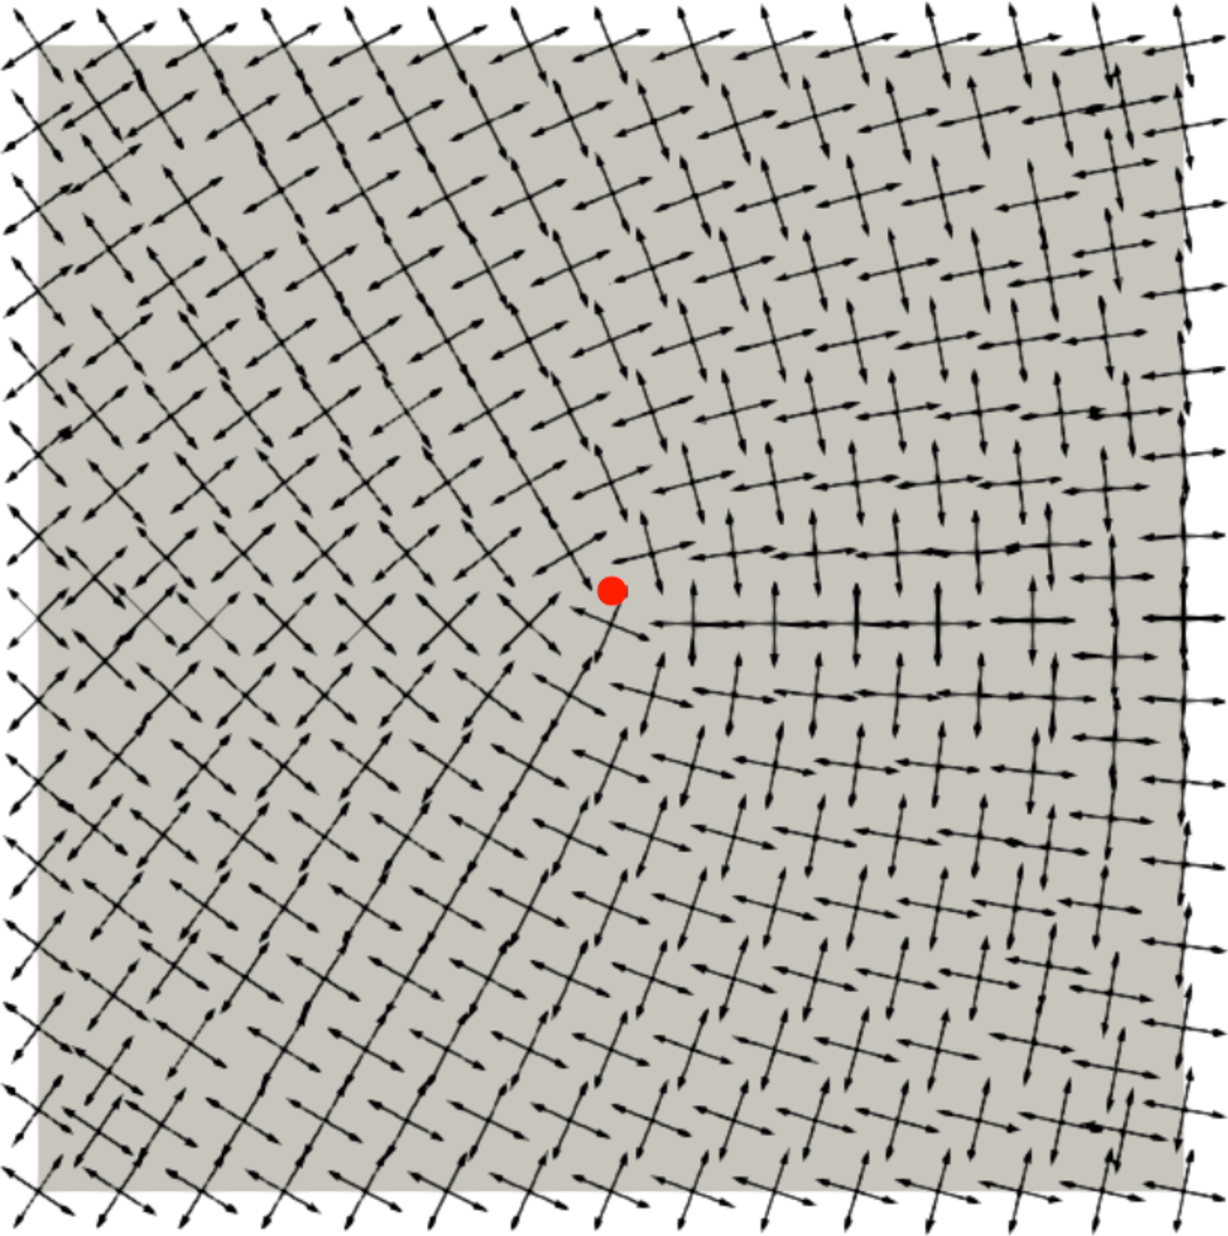
\includegraphics[scale=0.1765]{images/index_025.pdf}
  \hfill
  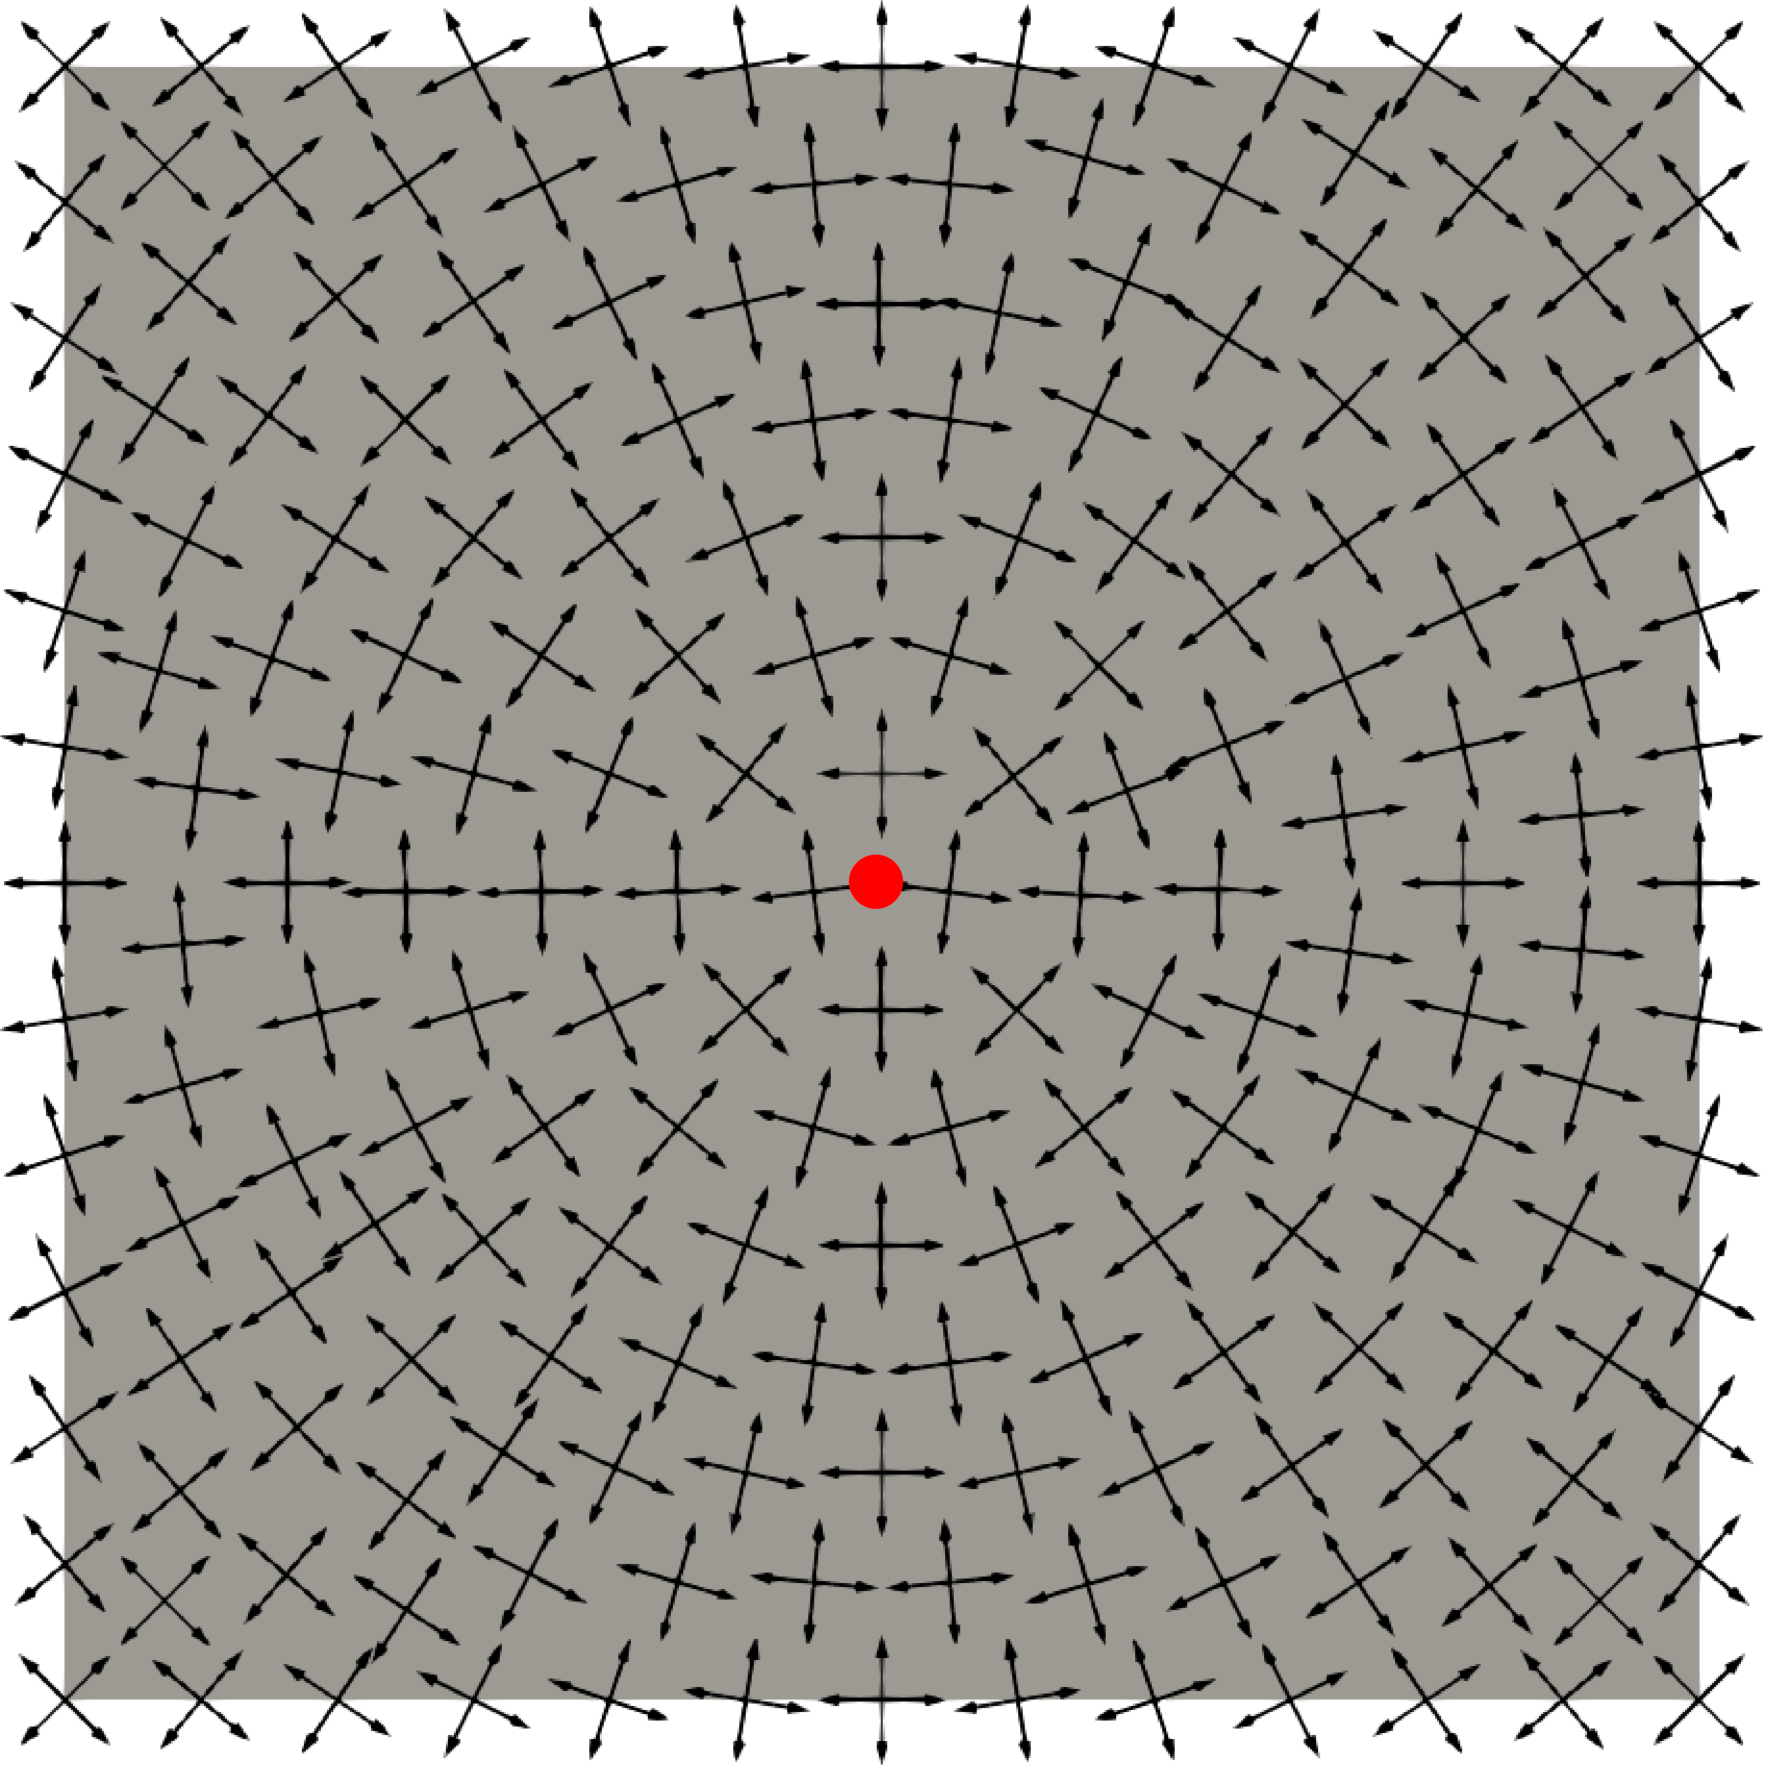
\includegraphics[scale=0.1765]{images/index_1.pdf}
  \caption{Gauche: $id_{\bar{u}}(p)=-\frac{1}{4}$, milieu: $id_{\bar{u}}(p)=\frac{1}{4}$, droite: $id_{\bar{u}}(p)=1$}
  \label{fig:index_illustration}
\end{figure}

Après avoir énoncé cette définition, on peut se demander comment l'indice d'un point évolue lorsqu'on effectue la rotation sur le champ de croix. Le résultat suivant fournit une réponse à cette interrogation.

\begin{proposition}
\label{prop:relation_u_Rthetau}
Soit $\bar{u}$ un champ de croix presque-$\mathcal{C}^1$ sur $\Omega$ et $\theta:\Omega \rightarrow \mathbb{R}$ une fonction de classe $\mathcal{C}^1$ sur $\Omega$, alors pour tout $p\in \Omega\backslash\partial\Omega,~id_{\bar{u}}(p)=id_{\mathbf{R}(\theta)\bar{u}}(p)$.
\end{proposition}

\begin{proof}
Posons $\bar{v}:=\mathbf{R}(\theta)\bar{u}$. Soit $p\in\Omega\backslash\partial\Omega$ et $\gamma:[0, 1]\longrightarrow\Omega$ un lacet dans $\Omega$ entourant $p$ et n'englobant aucun autre point singulier de $\bar{u}$. $\bar{u}$ étant un champ de croix presque-$\mathcal{C}^1$ sur $\Omega$, il existe donc $\theta_{\bar{u}}^\gamma\in\mathcal{C}^1(]0, 1[)$. Soit $\theta_{\bar{v}}^\gamma:=\theta\circ\gamma+\theta_{\bar{u}}^\gamma$. D'une part $\theta_{\bar{v}}^\gamma$ est de classe $\mathcal{C}^1$ sur $]0, 1[$ puisque $\theta\in\mathcal{C}^1(\Omega)$. D'autre part d'après la proposition \ref{prop:angular_cont}, $\theta_{\bar{v}}^\gamma(t)\equiv\theta(\gamma(t))+\theta_{\bar{u}}(\gamma(t))\pmod{\frac{\pi}{2}}$ et en utilisant la proposition \ref{prop:cont1} il vient que $\theta_{\bar{v}}^\gamma(t)\equiv\theta_{\bar{v}}(\gamma(t))\pmod{\frac{\pi}{2}}$. On a donc:
\begin{eqnarray*}
    id_{\bar{v}}(p)&=&\frac{1}{2\pi}\int_0^1 d\theta_{\bar{v}}^\gamma,\\
    &=&\frac{1}{2\pi}\left[\int_0^1 d(\theta\circ\gamma)+\int_0^1 d\theta_{\bar{u}}^\gamma\right],\\
    id_{\bar{v}}(p)&=&\frac{1}{2\pi}\left[\oint_\gamma d\theta+\int_0^1 d\theta_{\bar{u}}^\gamma\right].
\end{eqnarray*}
Or $\oint_\gamma d\theta=0$ puisque $\theta\in\mathcal{C}^1(\Omega)$. Autrement dit on a:
$$id_{\bar{v}}(p)=\frac{1}{2\pi}\int_0^1 d\theta_{\bar{u}}^\gamma=id_{\bar{u}}(p).$$
\end{proof}

Si $p\in\partial\Omega$ et le champ de croix $\bar{u}$ est aligné avec $\partial\Omega$, nous construisons une extension à la définition \ref{def:index} de la manière suivante: nous choisissons un lacet $\gamma\subset\Omega$ et paramétré sur $[0, 1]$ tel que $\gamma(0)=p=\gamma(1)$ et les vecteurs $\gamma'(0)$ et $\gamma'(1)$ sont tangents à $\partial\Omega$. On suppose de plus que $\gamma$ n'englobe pas d'autres points singulier de $\bar{u}$ à par $p$. L'indice de $p$ est alors donné par:

\begin{equation}
id^\partial_{\bar{u}}(p) = \frac{1}{2\pi}\left[\pi-\hat{p}+\lim\limits_{s\rightarrow 0}\int_s^{1-s}d\theta_{\bar{u}}^\gamma\right],
\label{eqn:Indexboundary}
\end{equation}
où $\hat{p}$ est la mesure de l'angle d'ouverture du bord en $p$. %Nous reviendrons sur cette définition dans la partie \ref{subsec:etude_de_la_methode} pour donner un lien entre l'index intérieur et l'index de bord.

\subsection{Théorème de Poincaré-Hopf}
\label{subsec:Poincare_Hopf}

Le théorème de Poincaré-Hopf constitue un résultat fondamental en topologie différentielle, établissant un lien profond entre les propriétés topologiques d'une variété différentielle compacte et les singularités d'un champ de vecteurs défini sur cette variété. Ce théorème fournit une manière précise de quantifier le nombre et le type de points singuliers d'un champ de vecteurs sur une variété compacte. En particulier, il établit une relation entre la somme des indices de ces points singuliers et la caractéristique d'Euler de la variété. Les auteurs de \cite{ray2008n} fournissent une adaptation de ce théorème aux champs de croix. Ainsi si $\bar{u}$ est un champ de croix presque-$\mathcal{C}^1$ sur $\Omega$ et aligné avec $\partial\Omega$ alors nous avons la formule suivante:

\begin{equation}
    \label{eqn:first_Poincare_Hopf}
    \sum_i id_{\bar{u}}(s_i)=\chi(\Omega),
\end{equation}
où la somme est celle des indices des points singuliers de $\bar{u}$ et $\chi(\Omega)$ est la caractéristique d'Euler de $\Omega$.

\begin{figure}[!h]
  \centering
  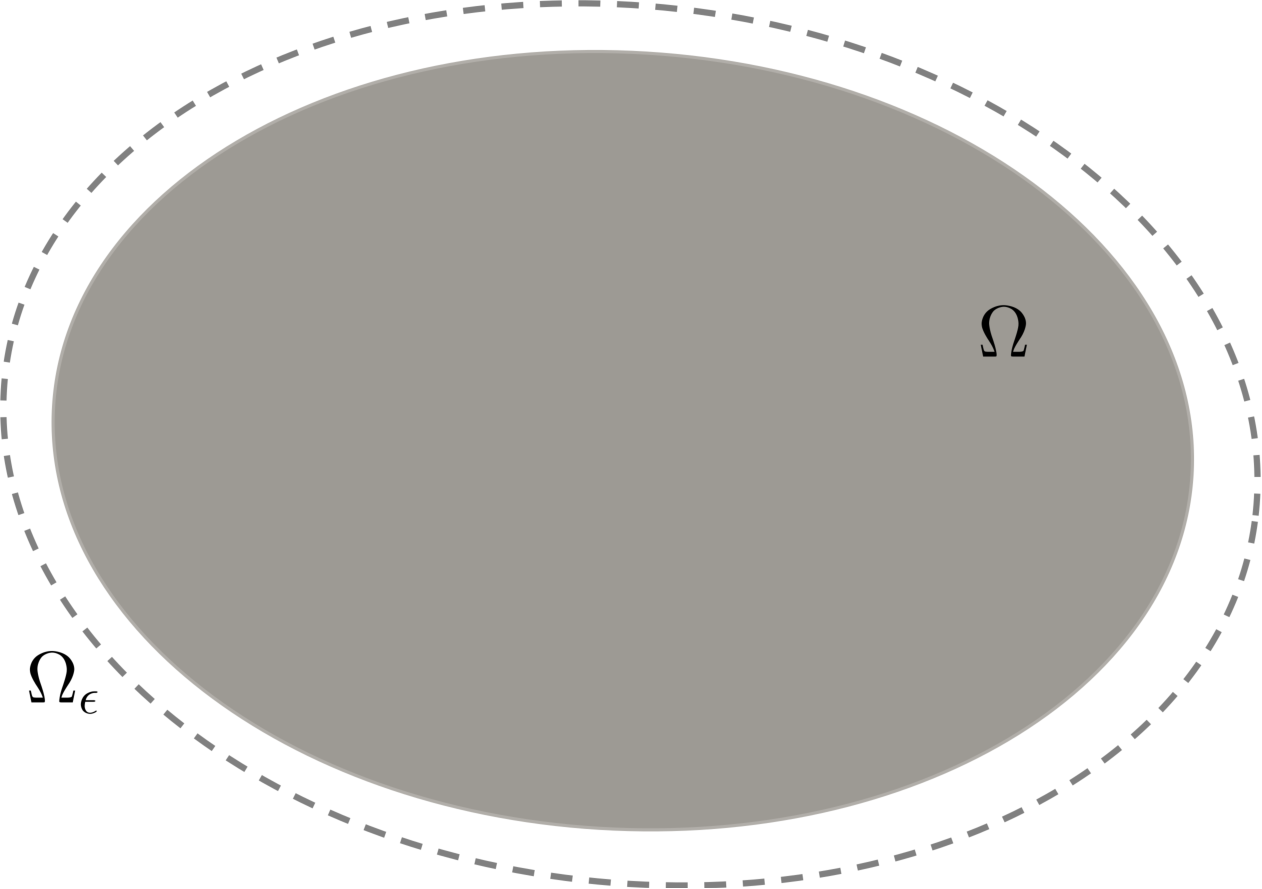
\includegraphics[scale=0.35]{images/Poincare_etendu.pdf}
  \caption{Extension du domaine pour la prise en compte des points singuliers de bord dans la formule de Poincaré-Hopf.}
  \label{fig:Poincare_etendu}
\end{figure}

Pour prendre en considération les champs de croix comportant des points singuliers situés sur la frontière du domaine, nous construisons un domaine $\Omega^\epsilon$ (voir la figure   \ref{fig:Poincare_etendu}) englobant $\Omega$ dont la frontiere est une isoline de valeur $\epsilon$ obtenu via la résolution de l'équation de la chaleur dans $\mathbb{R}^2\backslash\Omega$ et tel que $\partial\Omega^\epsilon\cap\Omega=\emptyset$. On construit ensuite le champ de croix $\bar{u}^\epsilon$ pour tout $p\in\Omega^\epsilon$ par:
$$
\bar{u}^\epsilon(p)=
\left\{
\begin{array}{ll}
\bar{u}(p)& \mbox{ si } p\in\Omega,\\[0.5cm]
\left\{\mathbf{R}\left(\displaystyle\frac{m\pi}{2}\right)f(p),~ m\in \mathbb{Z}\right\} & \mbox{ sinon },
\end{array}
\right.
$$
où pour tout $p\in\Omega^\epsilon\backslash\Omega$, $f$ désigne le vecteur gradient à l'isoline en $p$. Par construction, $\bar{u}^\epsilon$ est aligné sur le bord de $\Omega^\epsilon$ et $\mathcal{S}_{\bar{u}^\epsilon}\cap\partial\Omega^\epsilon=\emptyset$ Autrement dit, on a:
$$
\sum_{p\in\mathcal{S}_{\bar{u}^\epsilon}} id_{\bar{u}^\epsilon}(p)=\chi(\Omega^\epsilon).
$$
Or $\chi(\Omega^\epsilon)=\chi(\Omega)$ donc on a par le corollaire \ref{cor:sum_index}:
$$
\sum_{p\in\mathcal{S}_{\bar{u}^\epsilon}\backslash\partial\Omega} id_{\bar{u}^\epsilon}(p)+\sum_{p\in\mathcal{S}_{\bar{u}^\epsilon}\cap\partial\Omega} id_{\bar{u}^\epsilon}(p)=\chi(\Omega).
$$
Sachant que pour tout $p\in\partial\Omega$ on a $id_{\bar{u}^\epsilon}(p)=id^\partial_{\bar{u}}(p)$ alors
\begin{eqnarray}
    \label{eqn:poin_hopf_gen}
    \sum_{p\in\mathcal{S}_{\bar{u}}\backslash\partial\Omega} id_{\bar{u}}(p)+\sum_{p\in\mathcal{S}_{\bar{u}}\cap\partial\Omega} id^\partial_{\bar{u}}(p)&=&\chi(\Omega).
\end{eqnarray}
Nous posons alors l'équation \eqref{eqn:poin_hopf_gen} comme la généralisation de la formule de Poincaré-Hopf aux champs de croix aligné sur le bord du domaine et possédant des points singuliers de bord.


\begin{comment}
Pour prendre en considération les champs de croix comportant des points singuliers situés sur la frontière du domaine, nous introduisons le lemme suivant. Celui-ci établit une relation entre l'indice d'un point sur la frontière dans un champ de croix et l'indice intérieur de ce point dans un champ de croix étendu sur une zone englobant le point.
 \begin{lemma}
    \label{lem:lemme_poinc_hopf}
    Soit $\bar{u}$ un champ de croix presque-$\mathcal{C}^1$ sur $\Omega$ et aligné avec le bord de $\Omega$ et soit $p\in\partial\Omega$. Il existe un voisinnage $V_p\subset\mathbb{R}^2$ de $p$ et un champ de croix $\bar{v}$ presque-$\mathcal{C}^1$ sur $\Omega\cup V_p$ tel que $\mathcal{S}_{\bar{v}}=\mathcal{S}_{\bar{u}}$ et $id_{\bar{v}}(p) = id^\partial_{\bar{u}}(p)$.
\end{lemma}

\color{red}
\begin{proof}
    Soit $V_p=\bar{\mathcal{D}(p, \epsilon)}\backslash\mathring{\Omega}$ où $\bar{\mathcal{D}(p, \epsilon)}$ est le disque fermé centré en $p$ et de rayon $\epsilon>0$, tel que $\bar{\mathcal{D}(p, \epsilon)}\cap\partial\Omega=[pa]\cup[pb]$ avec $\{a, b\} = \partial\bar{\mathcal{D}(p, \epsilon)}\cap\partial\Omega$. $[pa]$ (respectivement $[pb]$) désigne le segment de droite $(pa)$ (respectivement $(pb)$) et les points $a$ et $b$ sont choisis de tel sorte que $\overrightarrow{ap}\wedge\overrightarrow{pb}>0$. On suppose de plus que $(V_p\cap\mathcal{S}_{\bar{u}})\backslash\{p\}=\emptyset$. Remarquons que $\Omega\cap V_p=[pa]\cap[pb]$. Soit $f$ la fonction définie pour tout $q\in V_p$ par:

    \begin{equation}
    f(q)=
    \left\{
    \begin{array}{ll}
        n(q) & \mbox{ si } q\in[pa],\\[0.5cm]
        \mathbf{R}\left(\alpha(\tau(q))\left(1-\displaystyle\frac{\pi}{2\pi-\hat{p}}\right)\right)n(\tau(q)) & \mbox{ sinon },
    \end{array}
    \right.
    \end{equation}
    où $\tau(q)=p+\|\overrightarrow{pq}\|.\|\overrightarrow{pa}\|^{-1}\overrightarrow{pa}$ et $\alpha(\tau(q))=\widehat{\tau(q)pq}$ est l'angle orienté entre les vecteurs $\overrightarrow{p\tau(q)}$ et $\overrightarrow{pq}$. Il est clair que $f$ est de classe $\mathcal{C}^1$ dans $V_p\backslash\{p\}$ puisque $\tau,\alpha\in\mathcal{C}^1(V_p\backslash\{p\}))$ et que la normale $n$ est $\mathcal{C}^1$ sur $]pa]$. Par conséquent, d'après la Propostion \ref{prop:cont1} le champ de croix $\bar{w}$ défini pour tout $q\in V_p$ par:
    \begin{equation}
    \bar{w}(q)=
    \left\{
    \begin{array}{ll}
        \bar{n}(p) & \mbox{ si } q=p,\\[0.5cm]
        \left\{\mathbf{R}\left(\displaystyle\frac{m\pi}{2}\right)f(q),~ m\in \mathbb{Z}\right\} & \mbox{ sinon },
    \end{array}
    \right.
    \end{equation}
    est presque-$\mathcal{C}^1$ sur $V_p\backslash\Omega$. Remarquons que pour tout $q\in\Omega\cap V_p$, $\bar{u}(q)=\bar{w}(q)$ puisque par définition si $q\in[pa]$, $\bar{u}(q)=\bar{w}(q)$ et pour tout $q\in]pb]$, $f(q)$maintenant $\bar{v}$, le champ de croix défini pour tout $q\in\Omega\cup V_p$ par:
    \begin{equation}
    \bar{v}(q)=
    \left\{
    \begin{array}{lcll}
    \bar{u}(q) & \mbox{ si } q\in\Omega,\\[0.5cm]
    \bar{w}(q) & \mbox{ sinon }.
    \end{array}
    \right.
    \end{equation}
    $\bar{v}$ est presque-$\mathcal{C}^1$ sur $\Omega\cup V_p$ avec $\mathcal{S}_{\bar{v}}=\mathcal{S}_{\bar{u}}$ et $id_{\bar{v}}(p)=id_{\bar{u}}(p)$. On a alors:
    \begin{eqnarray*}
        id_{\bar{w}}(p)&=&\int_{\partial V_p}d\theta_{\bar{w}},\\
        &=&\int_{\partial V_p\backslash\Omega}d\theta_{\bar{w}}+\int_{\partial V_p\backslash(\partial V_p\backslash\Omega)d\theta_{\bar{w}}}d\theta_{\bar{w}}\\\\
        id_{\bar{w}}(p)&=&\pi-\hat{p}+2\pi id^\partial_{\bar{u}}(p)-\pi+\hat{p}.
    \end{eqnarray*}
Ce qui montre que $id_{\bar{w}}(p)=id^\partial_{\bar{u}}(p)$.
\end{proof}
\color{black}
Grâce à ce lemme, la formule de Poincaré-Hopf \eqref{eqn:first_Poincare_Hopf} peut être écrite sur le domaine $\Omega\cup(\cup_{p\in\mathcal{S}_{\bar{u}}\cap\partial\Omega}V_p)$. Autrement dit, on a:
$$
\sum_{p\in\mathcal{S}_{\bar{w}}} id_{\bar{w}}(p)=\chi(\Omega\cup(\cup_{p\in\mathcal{S}_{\bar{u}}\cap\partial\Omega}V_p))
$$
Or $\chi(\Omega\cup(\cup_{p\in\mathcal{S}_{\bar{u}}\cap\partial\Omega}V_p))=\chi(\Omega)$ donc on a:
$$
\sum_{p\in\mathcal{S}_{\bar{w}}\backslash\partial\Omega} id_{\bar{w}}(p)+\sum_{p\in\mathcal{S}_{\bar{w}}\cap\partial\Omega} id_{\bar{w}}(p)=\chi(\Omega).
$$
D'après le lemme \ref{lem:lemme_poinc_hopf} on a $id_{\bar{w}}(p)=id^\partial_{\bar{u}}(p)$ pour tout $p\in\mathcal{}$:
\begin{eqnarray}
    \label{eqn:poin_hopf_gen}
    \sum_{p\in\mathcal{S}_{\bar{u}}\backslash\partial\Omega} id_{\bar{u}}(p)+\sum_{p\in\mathcal{S}_{\bar{w}}\cap\partial\Omega} id^\partial_{\bar{u}}(p)&=&\chi(\Omega).
\end{eqnarray}
Nous posons alors l'équation \eqref{eqn:poin_hopf_gen} comme la généralisation de la formule de Poincaré-Hopf aux champs de croix aligné sur le bord du domaine et possédant des points singuliers de bord.
\end{comment}

\subsection{Ligne de champ et séparatrices}

Le dernier point de cette section concerne un outil indispensable dans la technique de maillage qui est la construction de lignes de champ. En réalité, ces lignes seront les frontières des sous-régions générées par l'algorithme.
Comme pour les champs vectoriels, une ligne de champ d'un champ de croix $\bar{u}$ est définie comme une courbe continûment différentiable dans $\Omega$. Plus précisément, nous avons la définition suivante :

\begin{definition}
\label{def:SL}
Soit $\bar{u}$ un champ croisé presque-$\mathcal{C}^1$. Étant donné un point $p_0\in \Omega\backslash \mathcal{S}_{\bar{u}}$ et une direction $\overrightarrow{u_0}\in \bar{u}(p_0)$, une ligne de champ émanant de $p_0$ selon $\overrightarrow{u_0}\in \mathbb{R}^2$, notée par $SL{\bar{u}}(p_0,\overrightarrow{u_0})$, est la courbe $S$ telle que :

\begin{enumerate}
\item il existe $\pi_{\bar{u}}^S:\Omega\longrightarrow\mathbb{R}^2$ une application telle que $\pi_{\bar{u}}^S(p_0)=\overrightarrow{u_0}$ et pour tout $p\in Im S$ il existe un voisinnage $V_p$ de $p$ tel que:
\begin{equation}
\label{eqn:pi_u_S}
\pi_{\bar{u}}^S\in\mathcal{C}^1(V_p) \mbox{ et }  \forall q\in V_p, \pi_{\bar{u}}^S(q)\in \bar{u}(q),
\end{equation}
\item $S$ est une solution maximale dans $\Omega$ de l'équation différentielle
\begin{equation}
\label{eqn:streamline}
\frac{dS(t)}{dt}=\pi_{\bar{u}}^S(S(t)),t\in \mathbb{R} \text{ et }  S(0)=p_0.
\end{equation}
\end{enumerate}
\end{definition}

\begin{lemma}
\label{lem:def_streamline_lemma}
La courbe $SL_{\bar{u}}(p_0,\overrightarrow{u_0})$ proposée dans la définition~\ref{def:SL} est bien définie.
\end{lemma}

\begin{proof}
Pour établir ce lemme, nous construisons d'abord l'application $\pi$ restreinte au voisinage de $p$ et procédons ensuite à la construction de la ligne de champ restreinte au voisinage de $p$. La ligne de champ complète est ensuite formée en étendant itérativement cette construction à chaque voisinage successif (voir figure \ref{fig:streamline_construction}).\
\begin{figure}[!h]
\centering
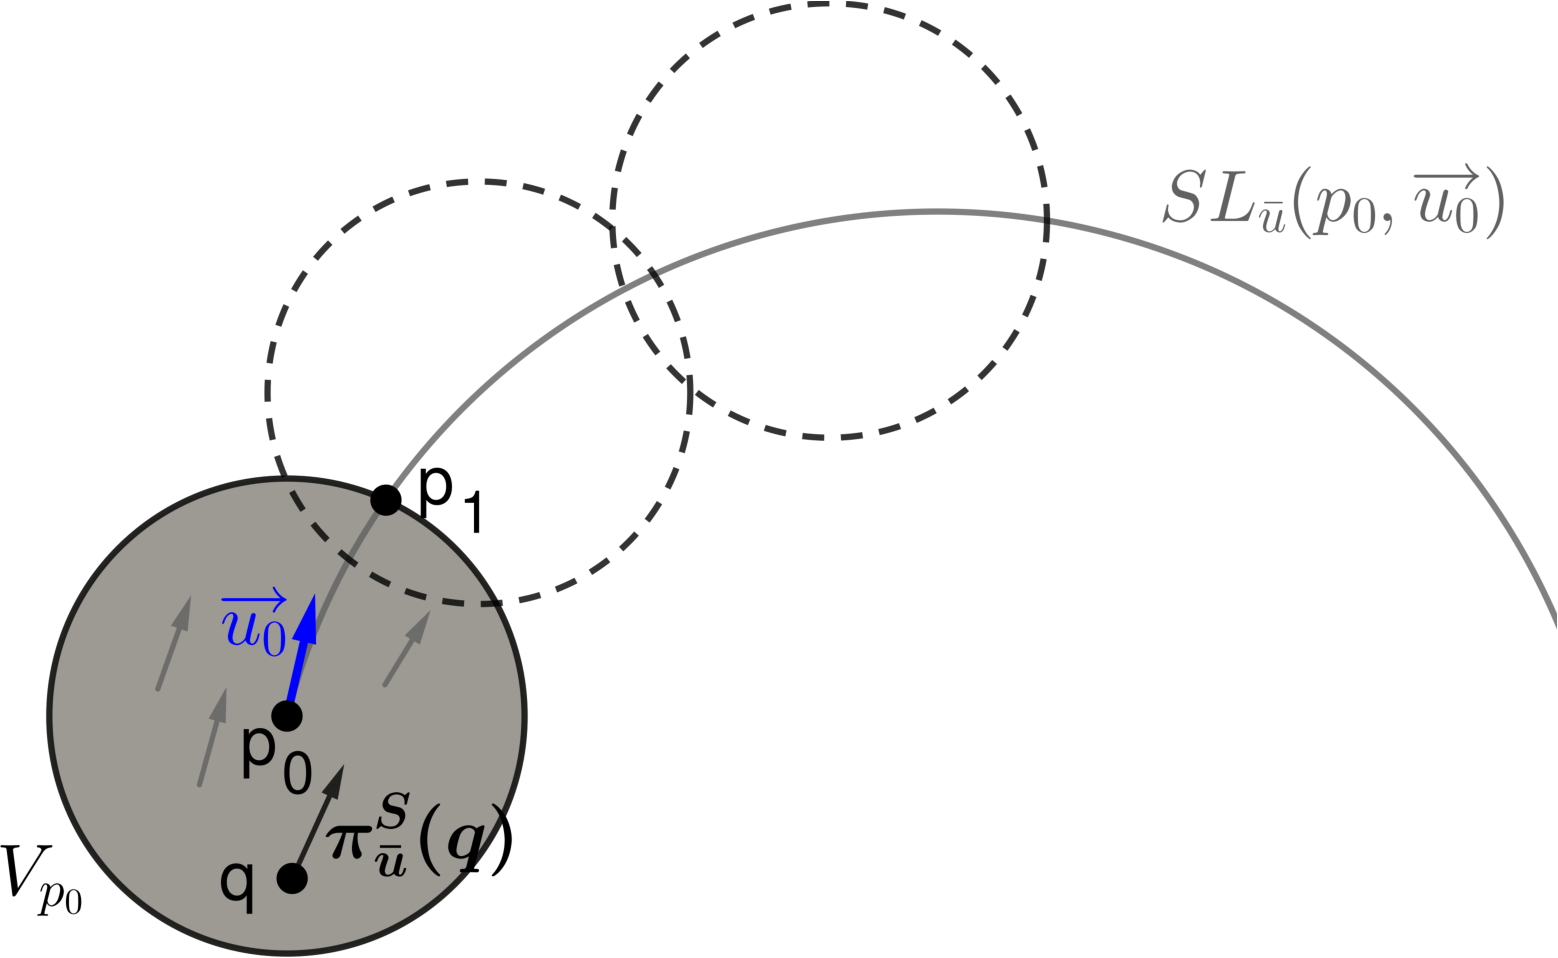
\includegraphics[scale=0.45]{images/streamline_construction.pdf}
\caption{Illustration de la preuve du lemme \ref{lem:def_streamline_lemma}.}
\label{fig:streamline_construction}
\end{figure}

\paragraph{Définition d'un champ de vecteur de classe $\mathcal{C}^1$ dans un voisinnage de $p_0$.} D'après la proposition \ref{prop:angular_cont}, il existe une application $\theta_{\bar{u}}^{V_{p_0}}$ de classe $\mathcal{C}^1$ dans un voisinnage $V_{p_0}$ de $p_0$ telle que pour tout $q\in V_{p_0}$, $\theta_{\bar{u}}^{V_{p_0}}(q)\equiv\theta_{\bar{u}}(q)\pmod{\frac{\pi}{2}}$. Il vient alors qu'il existe $m\in\mathbb{Z}$ tel que l'application $\tau_{p_0}:=\mathbf{R}(\theta_{\bar{u}}^{V_{p_0}}+m\frac{\pi}{2})(1, 0)$ est un champ de vecteur de classe $\mathcal{C}^1$ sur $V_{p_0}$ vérifiant $\tau_{p_0}(p_0)=\overrightarrow{u_0}$.

\paragraph{Construction de la restriction de $\pi_{\bar{u}}^S$ au voisinage de $p_0$.}
Montrons que si $\pi_{\bar{u}}^S\in\mathcal{C}^1(V_{p_0})$ tel que $\pi_{\bar{u}}^S(p_0)=\overrightarrow{u_0}$ satisfaisant \eqref{eqn:pi_u_S} et \eqref{eqn:streamline}, alors $\pi_{\bar{u}}\circ S=\tau_{p_0}\circ S$ sur $V_{p_0}$. Supposons qu'il existe $t\in\mathbb{R}$ tel que $p'=S(t)\in V_{p_0}$ et $\pi_{\bar{u}}^S\circ S(t)\neq\tau_{p_0}\circ S(t)$.

Soit $\epsilon>0$. $\tau_{p_0}$ étant continue sur $V_{p_0}$, pour $p$ assez proche de $p_0$, on a:
$$|\tau_{p_0}(p)-\pi^S_{\bar{u}}(p_0)|=|\tau_{p_0}(p)-\tau_{p_0}(p_0)|\leq\epsilon.$$
Par inégalité triangulaire, il vient que:
$$|\pi^S_{\bar{u}}(p)-\pi^S_{\bar{u}}(p_0)|\geq|\tau_{p_0}(p)-\pi^S_{\bar{u}}(p^)|-\epsilon.$$
Or on sait que $\pi^S_{\bar{u}}(p')\in{\bar{u}}(p')$, $\tau_{p_0}(p')\in{\bar{u}}(p')$ et $\pi_{\bar{u}}^S(p')\neq\tau_{p_0}(p')$, ce qui implique que $\pi^S_{\bar{u}}(p')=R(k\pi/2)\tau_{p_0}(p')$ où $k\in\mathbb{Z}\backslash 4\mathbb{Z}$, et donc que $|\pi^S_{\bar{u}}(p')-\tau_{p_0}(p')|\geq\sqrt{2}$. Par conséquent, si $p'$ est assez proche de $p_0$, en l'occurrence nous prenons $p'\in\mathcal{B}(p_0,\epsilon)$ on a:
\[
\epsilon \geq |p' - p_0| \geq |\pi^S_{\bar{u}}(p') - \pi^S_{\bar{u}}(p_0)| \geq |\sqrt{2} - \epsilon|,
\]
puisque $\pi^S_{\bar{u}}$ est uniformément continue avec une constante de $1$. Cela conduit à une contradiction en prenant $\epsilon = \sqrt{2}/4$. % contredit le fait que $\pi_{\bar{u}}^S\in\mathcal{C}^1(V_{p_0})$.

Si $p' \notin \mathcal{B}(p_0, \epsilon)$, on choisit un nouveau point $p_0^1$ à la frontière de cette boule. Ensuite, on établit le raisonnement précédent avec ce nouveau point si $p' \in \mathcal{B}(p_0^1, \epsilon)$. Dans le cas contraire, on avance itérativement jusqu'à avoir $p'$ dans la boule.



\paragraph{Construction de la restriction de la ligne de courant au voisinage de $p$.}
Selon ce qui a été établi précédemment, $S$ satisfait l'équation suivante dans $V_{p_0}$ :\begin{equation}
\label{eqn:streamline_in_V}
\frac{dS(t)}{dt}=\tau_{p_0}(S(t)),t\in \mathbb{R} \text{ et }  S(0)=p_0.
\end{equation}
Nous obtenons la séparatrice $S$ en intégrant l'équation \eqref{eqn:streamline_in_V} jusqu'à ce que $u(s(t))=0$ ou que $s(t)\in\partial V_{p_0}$ pour $t>0$ (respectivement, $t<0$). Sans perte de généralité, notons $t_1$ le moment auquel cela se produit et $S(t_1)=p_1$.\\
\begin{itemize}
\item[-] Si $\bar{u}(p_1)=0$, alors $S(t)$ est la ligne de champ construite existe et est unique,\\
\item[-] Sinon, nous pouvons étendre l'ensemble $S$ en répétant la construction précédemment décrite dans un voisinage de $p_1$. Cela implique de définir un champ vectoriel continu à proximité de $p_1$ et de construire la ligne de champ en fonction de ce champ étendu. En appliquant itérativement ce processus dans chaque voisinage, nous pouvons étendre et affiner progressivement la ligne de courant, en garantissant sa régularité dans tout le domaine.
\end{itemize}
\end{proof}


\begin{remark}
Notons que si $\bar{u}$ est aligné avec la frontière, alors pour tout $p\in \partial \Omega \backslash \mathcal{S}_{\bar{u}}$ tel que la normale extérieure unitaire $n(p)$ au point $p$, est définie, nous avons $SL{\bar{u}}\left(p,\mathbf{R}\left(\pm \frac{\pi}{2}\right)n(p)\right) \subset \partial \Omega$.
\end{remark}

\begin{definition}[Séparatrice] \label{def:sep}
Une séparatrice dans un champ de croix est une ligne de champ qui commence ou se termine en un point singulier.
\end{definition}

Cette définition d'une séparatrice induit un problème bien connu dans les équations différentielles ordinaires : comment tracer une ligne de champ à partir d'un point singulier donné ? Cette question peut être difficile étant donné que $\bar{u}(p)={0}$ pour tout $p\in \mathcal{S}_{\bar{u}}$. Cependant, nous proposons le résultat suivant qui sera utilisé par la suite pour résoudre ce problème.
\begin{proposition}
\label{prop:stream_from_interior_sing}
Soit $\bar{u}$ un champ de croix presque-$\mathcal{C}^1$ et $p\in \Omega\backslash\partial\Omega$. Soit $V_p\subset\Omega$ un voisinnage de $p$ tel que le bord $\partial V_p$ de $V_p$ est de classe $\mathcal{C}^1$ et $\partial V_p\cap\mathcal{S}_{\bar{u}}=\emptyset$. On suppose de plus que $V_p$ est étoilé par rapport à $p$. Alors il existe un champ de croix $\bar{v}$ tel que:\\[-0.3cm]
\begin{enumerate}
\item $\bar{v}$ est presque-$\mathcal{C}^1$ sur $\Omega$,\\[-0.3cm]
\item $\mathcal{S}_{\bar{v}}\cap V_p =\{p\}$ et $id_{\bar{v}}(p)=\sum_{q\in \mathcal{S}_{\bar{u}}\cap V_p} id_{\bar{u}}(q)$,\\[-0.3cm]
\item pour tout $q\in \partial V_p$ tel que $\overrightarrow{v_q}:=\overrightarrow{pq}.\|\overrightarrow{pq}\|^{-1}\in \bar{u}(q)$, le point $p$ appartient à la ligne de champ $SL_{\bar{v}}(q,\overrightarrow{v_q})$.\\[-0.3cm]
\end{enumerate}
\end{proposition}

\begin{proof}
Soit $\bar{v}$ défini pour tout $q\in\Omega$ par :
\begin{equation}
\label{eqn:equa_etoilage}
\bar{v}(q)=
\left\{
\begin{array}{ll}
0&\mbox{ si }q=p\\[0.25cm]
\bar{u}(q)&\mbox{ si } q\notin V_p,\\[0.25cm]
\bar{u}\circ\pi(q)&\mbox{ sinon},
\end{array}
\right.
\end{equation}
où $\pi$ est défini pour tout $q\in V_p\backslash\{p\}$ par l'intersection de la demi-droite $[pq)$ avec la courbe $\partial V_p$ (voir la figure \ref{fig:illustr_etoilage}):
\begin{equation*}
\left\{
\begin{array}{ll}
\pi(q)=p+\displaystyle\frac{\overrightarrow{\|p\pi(q)\|}}{\overrightarrow{\|pq\|}}\overrightarrow{pq},\\[0.5cm]
\pi(q)\in\partial V_p.
\end{array}
\right.
\end{equation*}
\begin{figure}[!h]
\centering
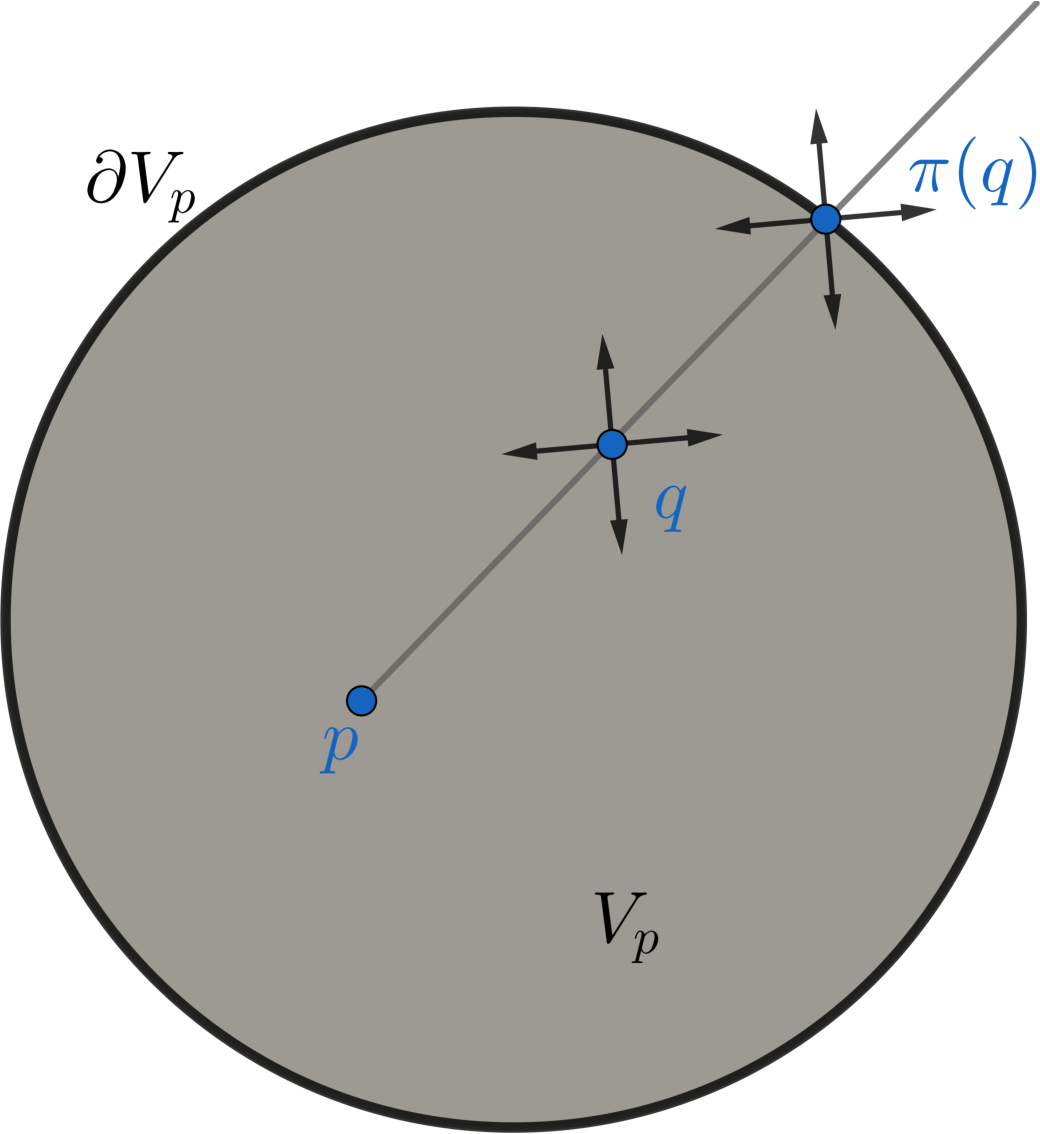
\includegraphics[scale=0.4]{images/illustr_etoilage.pdf}
\caption{Illustration de la construction du champ de croix $\bar{v}$ dans $\partial V_p$.}
\label{fig:illustr_etoilage}
\end{figure}
Notons que $\pi$ est bien défini. En effet, puisque $V_p$ est étoilé et que $\partial V_p$ est de classe $\mathcal{C}^1$, alors pour tout $q\in V_p\backslash\{p\}$, il existe un unique point $\pi(q)\in\partial V_p$. Nous montrons que $\bar{v}$ est presque continue dans $\Omega$ en démontrant cette propriété successivement dans $V_p$, dans $\Omega\backslash V_p$, et sur $\partial V_p$.\\
\begin{itemize}
\item Dans $V_p$ (voir Figure \ref{fig:v_bar_almost_continuous}) : Soit $x \in V_p$ fixé et $\epsilon > 0$. Nous voulons montrer qu'il existe $\eta > 0$ tel que pour tout $y \in V_p$, si $|x-y|\leq\eta$, alors $|\widetilde{g}(x)-\widetilde{g}(y)|\leq\epsilon$. Puisque $g'$ est continue, il existe $\eta_g$ tel que pour tout $x', y' \in \partial V_p$, si $|x'-y'|\leq\eta_g$, alors $|g'(x')-g'(y')|\leq\epsilon$. Soit $t^\pm=t_x\pm\eta_g$ avec $\gamma(t_x)=\pi(x)$, et soit $\mathcal{H}_x=V_p\cap\mathrm{C}(\gamma(t^-), p, \gamma(t^+))$, où $\mathrm{C}(\gamma(t^-), p, \gamma(t^+))$ désigne la région du plan délimitée par les demi-droites $[p\gamma(t^-))$ et $[p\gamma(t^+))$. Puisque $p\in V_p$, nous avons $\mathcal{H}_x \neq\emptyset$. De plus, $\mathcal{H}_x$ est ouvert par construction. Cela implique l'existence d'un certain $\eta>0$ tel que $\mathcal{B}(x,\eta)\subset \mathcal{H}_x$, et pour tout $y$ tel que $|x-y|\leq\eta$, nous avons $|\pi(x)-\pi(y)|\leq\eta_g$. Ceci prouve la continuité de $\pi$ et donc la continuité de $\widetilde{g}$ puisque $\bar{u}$ est continue dans $V_p$.\\
\item Dans $\Omega\backslash V_p$ : $\bar{v}$ est presque continue dans $V_p$ par définition.\\
\item Sur $\partial V_p$ : $\bar{v}$ est presque continue sur $\partial V_p$ grâce à une jonction continue de deux fonctions continues.\\
\end{itemize}
\begin{figure}[!h]
\centering
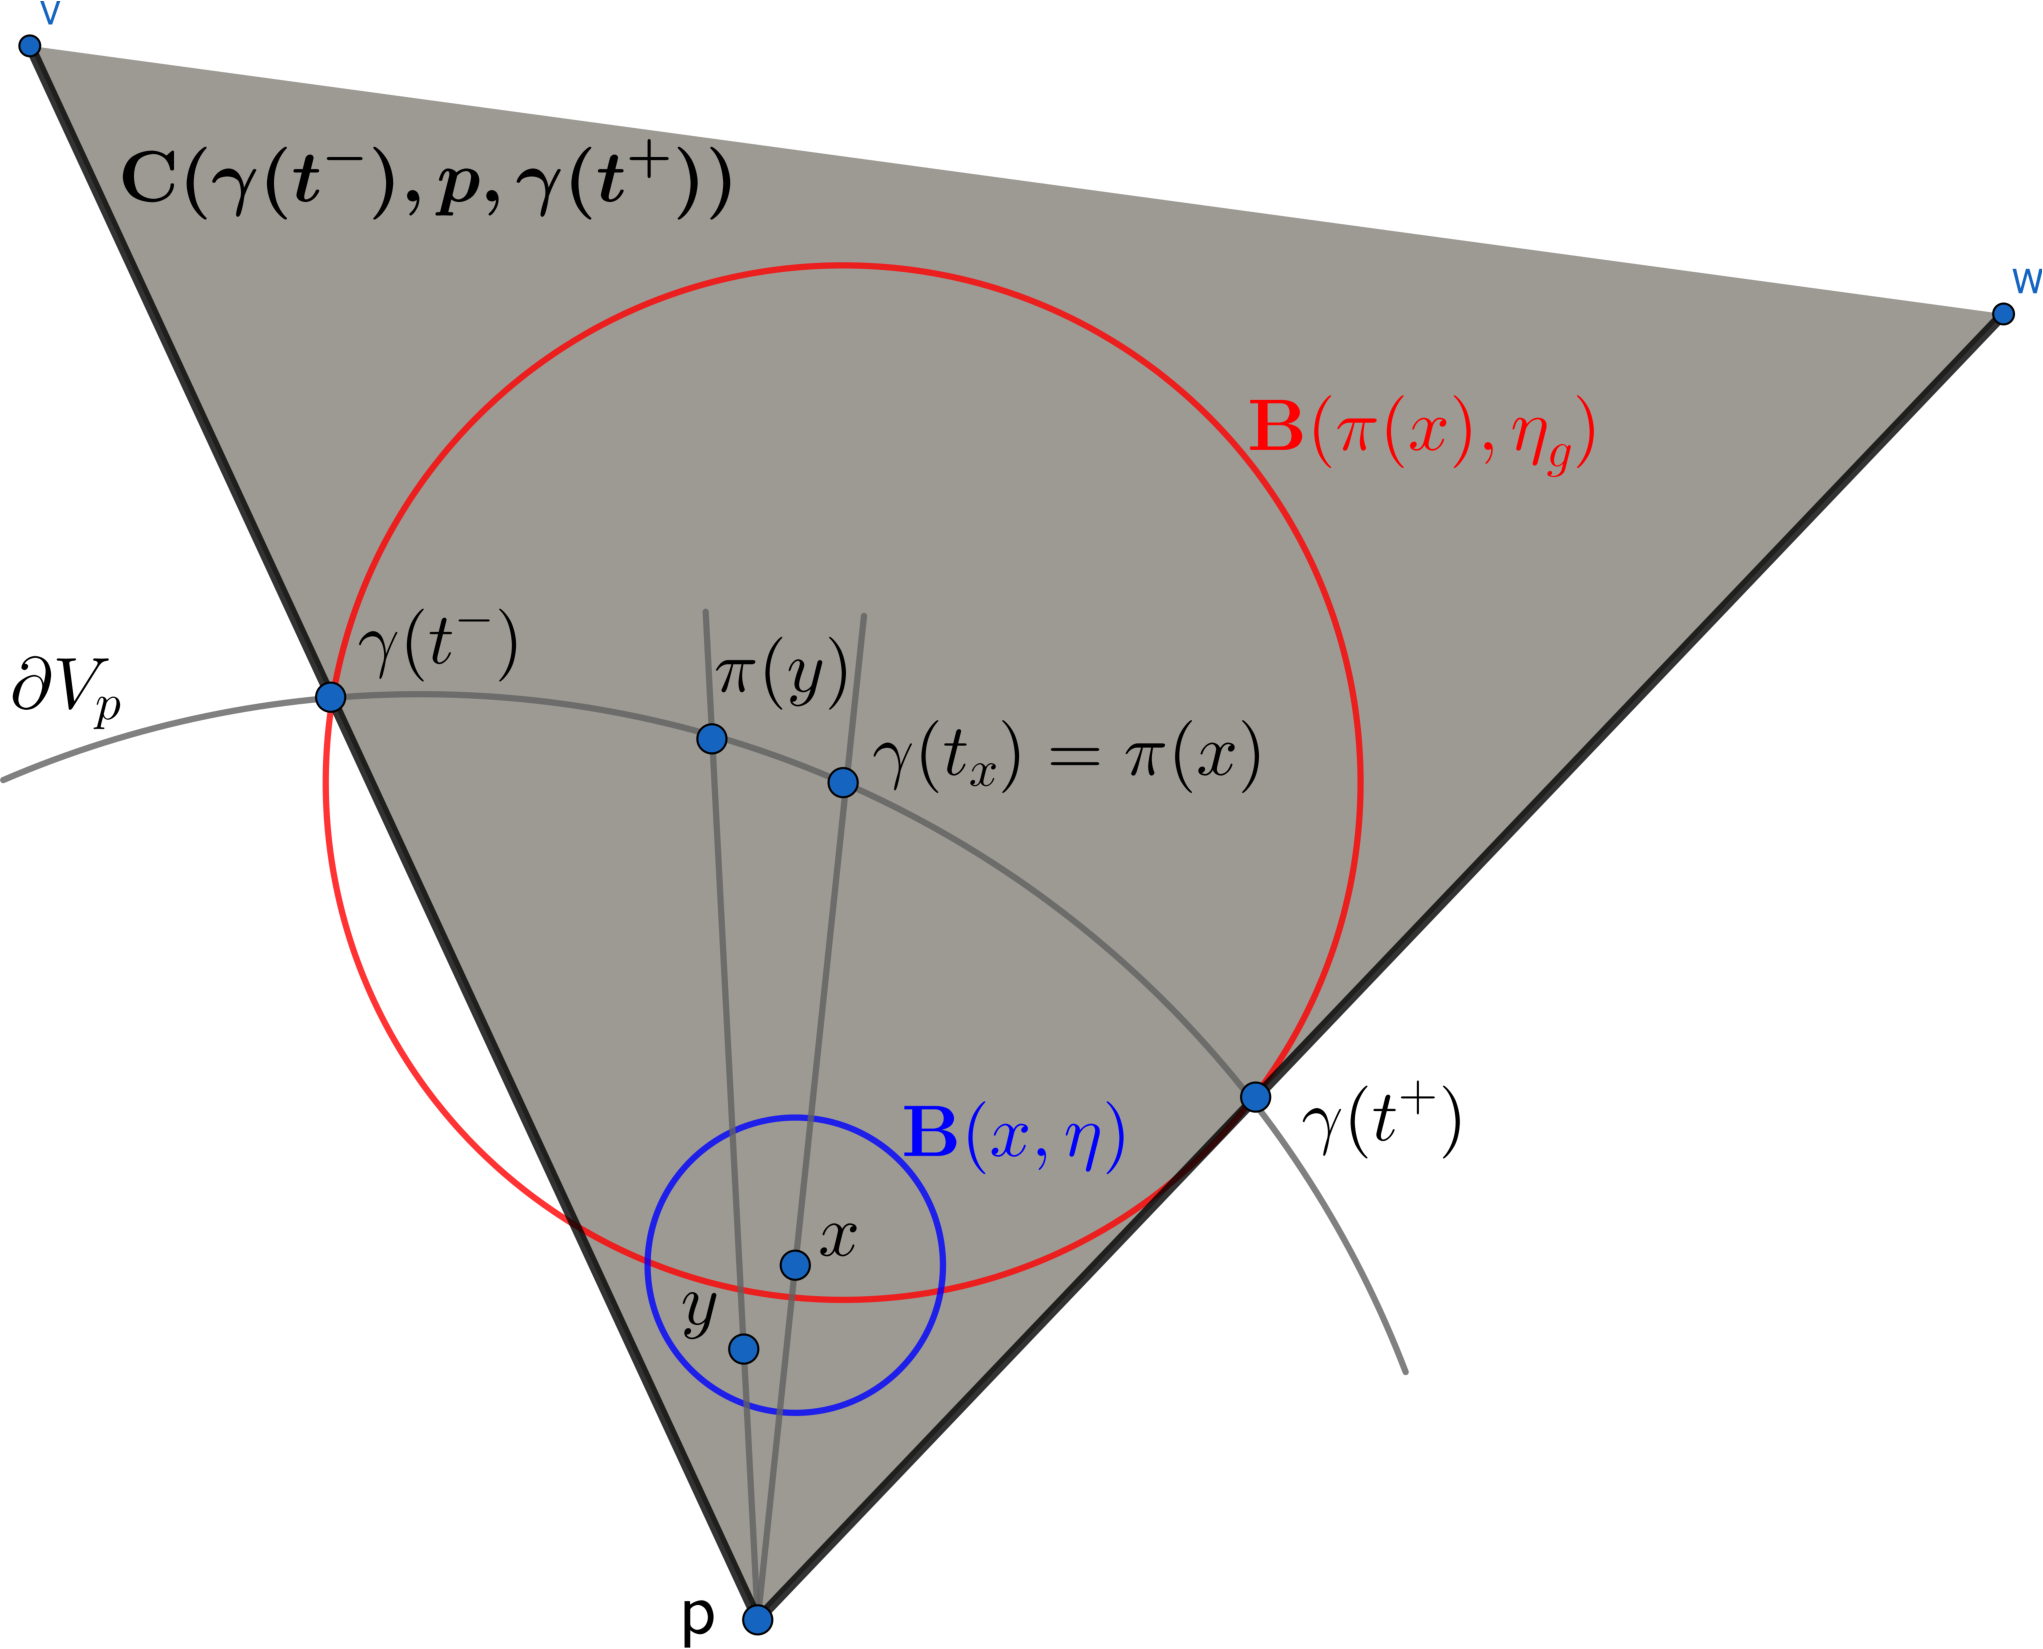
\includegraphics[scale=0.35]{images/v_bar_almost_continuous_++.pdf}
\caption{Illustration of the construction of the restriction of $\pi$}
\label{fig:v_bar_almost_continuous}
\end{figure}

Pour montrer que $\bar{v}$ est presque-$\mathcal{C}^1$ dans $V_p\backslash\{p\}$, il suffit de montrer que $\pi$ est $\mathcal{C}^1$ puisque $\bar{u}$ est $\mathcal{C}^1$ sur $\partial V_p$. Pour ce faire, nous essayons de calculer la differentielle de $\pi$ et de montrer qu'elle est $\mathcal{C}^0$. Soit $q\in V_p$ et $h\in\mathbb{R}^2$. Calculons $\pi(q+h)$.
\begin{eqnarray*}
    \pi(q+h)&=&p+\frac{\|\overrightarrow{p\pi(q+h)}\|}{\|\overrightarrow{p(q+h)}\|}\overrightarrow{p(q+h)}\\[0.2cm]
    &=&p+\left(\frac{\|\overrightarrow{p\pi(q)}\|}{\|\overrightarrow{pq}\|}+\frac{<\overrightarrow{p\pi(q)}, (\nabla\pi(q).h)>}{\|\overrightarrow{pq}\|\|\overrightarrow{p\pi(q)}\|}\right)\left(1-\frac{\overrightarrow{pq}.h}{\|\overrightarrow{pq}\|^2}\right)\left(\overrightarrow{pq}+h\right) + o(h^2)\\[0.2cm]
    &=&\pi(q)+\frac{<\overrightarrow{p\pi(q)}, (\nabla\pi(q).h)>}{\|\overrightarrow{pq}\|\|\overrightarrow{p\pi(q)}\|}\overrightarrow{pq}-\frac{\|\overrightarrow{p\pi(q)}\|}{\|\overrightarrow{pq}\|}\frac{\overrightarrow{pq}.h}{\|\overrightarrow{pq}\|^2}\overrightarrow{pq}+\frac{\|\overrightarrow{p\pi(q)}\|}{\|\overrightarrow{pq}\|}h+o(h^2)\\[0.2cm]
    \pi(q+h)&=&\pi(q)+\frac{<\overrightarrow{p\pi(q)}, (\nabla\pi(q).h)>}{\|\overrightarrow{pq}\|\|\overrightarrow{p\pi(q)}\|}\overrightarrow{pq}+\frac{\|\overrightarrow{p\pi(q)}\|}{\|\overrightarrow{pq}\|}\left(\frac{\overrightarrow{pq}.h}{\|\overrightarrow{pq}\|^2}\overrightarrow{pq}+h\right)+o(h^2)
\end{eqnarray*}

En posant $e_q=\displaystyle\frac{\overrightarrow{pq}}{\|\overrightarrow{pq}\|}$ et $\lambda_q=\displaystyle\frac{\|\overrightarrow{p\pi(q)}\|}{\|\overrightarrow{pq}\|}$ on obtient:

\begin{eqnarray*}
    \pi(q+h) = \pi(q)+<e_q,\nabla\pi(q).h>e_q+\lambda_q(-(e_q.h)e_q+h)+o(h^2).
\end{eqnarray*}
Posons $L(h)=<e_q,\nabla\pi(q).h>e_q+\lambda_q(-(e_q.h)e_q+h)$. La composante de $L(h)$ suivant $\overrightarrow{e_q^\perp}$ est donnée par $X=L(h).e_q^\perp=\lambda_q(h.e_q^\perp)$ qui est continue en $q$. Nous cherchons ensuite la composante suivant $\overrightarrow{e_q}$: soit $\gamma$ une paramétrisation de $\partial V_p$ sur $I\subset\mathbb{R}$. Puisque $\pi(q+h),\pi(q)\in\partial V_p$, il existe $t_1, t_2\in I$ tel que $\pi(q)=\gamma(t_1)$ et $\pi(q+h)=\gamma(t_2)$. $\gamma$ étant $\mathcal{C}^1$, il existe une fonction dépendant de $h$ notée $m(h)$ telle que $\pi(q+h)-\pi(q)=m(h).\overrightarrow{t}+o(h^2)$ avec $\overrightarrow{t}=\gamma'(t_1).\|\gamma'(t_1)\|^{-1}$. Ce qui implique que $L(h)$ est colinéaire au vecteur $\overrightarrow{t}$. Il vient alors que:
$$
X=L(h).\overrightarrow{e_q^\perp}=\|L(h)\|\cos{\alpha},\mbox{ avec }\cos{\alpha}=\overrightarrow{t}.\overrightarrow{e_q^\perp}.
$$
Autrement dit, la composante de $L(h)$ suivant $e_q$ notée $Y$ est donnée par:
$$
Y=\pm\sqrt{\|L(h)\|^2-X^2}=\frac{\pm 1}{\cos{\alpha}}\sqrt{X^2(1+\cos^2\alpha)},
$$
\begin{comment}
\begin{figure}[!h]
\centering
\includegraphics[scale=0.4]{img/im_future.png}
\caption{}%Illustration de la construction de la restriction de $\pi$.}
%\label{fig:v_bar_almost_continuous}
\end{figure}
\end{comment}
avec $\cos{\alpha}\neq 0$. Si $\cos{\alpha}= 0$ alors on a $\overrightarrow{t}.\overrightarrow{e_q^\perp}=0$ ce qui exclut puisque $V_p$ est étoilé par rapport à $p$. Finalement, on a $L(h)=X\overrightarrow{e_q^\perp}+ Y\overrightarrow{e_q}$ avec $X$ et $Y$ linéaire en $h$ et continue en $q$. Par conséquent, $\pi$ est bien de classe $\mathcal{C}^1$.\\\\
2.\quad Pour tout $q\in V_p\backslash\{p\}$, $\bar{v}(q)\neq 0$ et $\bar{v}(p)=0$. Par conséquent, $\mathcal{S}_{\bar{v}}\cap V_p=\{p\}$. Soit $\gamma$ une paramétrisation de $\partial V_p$ sur $[0, 1]$. Sachant que l'indice de $p$ dans le champ de croix $\bar{v}$ ne dépend pas du chemin, on peut écrire que:
$$id_{\bar{v}}(p)=\frac{1}{2\pi}\int_{\partial V_p}d\theta_{\bar{v}}.$$
Or par construction, on a $\bar{v}=\bar{u}$ sur $\partial V_p$ donc on a:
$$id_{\bar{v}}(p)=\frac{1}{2\pi}\int_{\partial V_p}d\theta_{\bar{u}}=\sum_{q\in\mathcal{S}_{\bar{u}}\cap V_p}id_{\bar{u}}(q).$$\\\\
3.\quad Soit $q\in\partial V_p$ tel que $\overrightarrow{v_q}:=\overrightarrow{pq}.\|\overrightarrow{pq}\|^{-1} \in \bar{u}(q)$. Alors pour tout $p'\in~]pq)\cap V_p$ on a $\overrightarrow{v_q}\in\bar{v}(p')$. Par conséquent, pour tout $p'\in]pq]$ on a $p'\in SL_{\bar{v}}(q,\overrightarrow{v_q})$. Ainsi en passant à la limite avec $p'\longrightarrow p$ on a $p\in SL_{\bar{v}}(q,\overrightarrow{v_q})$.
\end{proof}

En extension de la proposition \ref{prop:stream_from_interior_sing}, nous introduisons la proposition suivante, qui décrit une procédure pour tracer une ligne de courant à partir d'un point singulier spécifié sur la frontière.

\begin{proposition}
\label{prop:stream_from_bord_sing}
Soit $\bar{u}$ un champ de croix presque-$\mathcal{C}^1$ et $p\in\partial\Omega$. Considérons un voisinage $V_p\subset\Omega$ de $p$ tel que $p\in\partial V_p$ et $\partial V_p$ soit de classe $\mathcal{C}^1$. On suppose de plus que $(\partial V_p\backslash\{p\})\cap\mathcal{S}_{\bar{u}}=\emptyset$ et que $V_p$ est étoilé par rapport à $p$. Alors, il existe un champ de croix $\bar{v}$ tel que:
\begin{enumerate}
\item[1.] $\bar{v}$ est presque-$\mathcal{C}^1$ sur $\Omega$,\\[-0.3cm]
\item[2.] pour tout $q\in \partial V_p$ tel que $\overrightarrow{v_q}:=\overrightarrow{pq}.\|\overrightarrow{pq}\|^{-1}\in \bar{u}(q)$, le point $p$ appartient à la ligne de champ $SL_{\bar{v}}(q,\overrightarrow{v_q})$.\\[-0.3cm]
\end{enumerate}
De plus, si $\partial V_p$ est tangent à $\partial\Omega$ en p, alors on a:
\begin{enumerate}
\item[3.] $\mathcal{S}_{\bar{v}}\cap V_p =\{p\}$ et $id^\partial_{\bar{v}}(p)=\sum_{q\in \mathcal{S}_{\bar{u}}\cap V_p} id_{\bar{u}}(q)$.\\[-0.3cm]
\end{enumerate}
\end{proposition}

\begin{proof}
Soit $\bar{v}$ défini pour tout $q\in\Omega$ par l'équation \eqref{eqn:equa_etoilage}:\\\\
1.\quad La proposition \ref{prop:stream_from_interior_sing} montre que $\bar{v}$ est presque-$\mathcal{C}^1$ sur $\Omega$.\\\\
2.\quad Voir la preuve de la proposition \ref{prop:stream_from_interior_sing}.\\\\
3.\quad Supposons maintenant que $\partial V_p$ est tangent à $\partial V_p$ en p. Pour tout $q\in V_p\backslash\{p\}$, $\bar{v}(q)\neq 0$ et $\bar{v}(p)=0$. Par conséquent, $\mathcal{S}_{\bar{v}}\cap V_p=\{p\}$. Soit $\gamma$ une paramétrisation de $\partial V_p$ sur $[0, 1]$ avec $\gamma(0)=p=\gamma(1)$. Puisque $\partial V_p$ est tangent à $\partial\Omega$ en p, les vecteurs $\gamma'(0)$ et $\gamma'(1)$ sont tangents à $\partial\Omega$. On a donc par le corollaire \ref{cor:sum_index}:
$$
id^\partial_{\bar{v}}(p)=\frac{1}{2\pi}\left[\pi-\hat{p}+\lim\limits_{s\rightarrow 0}\int_s^{1-s}d\theta_{\bar{v}}^\gamma\right].
$$
Or par construction, on a $\bar{v}=\bar{u}$ sur $\partial V_p$ donc on a:
$$id^\partial_{\bar{v}}(p)=\frac{1}{2\pi}\left[\pi-\hat{p}+\lim\limits_{s\rightarrow 0}\int_s^{1-s}d\theta_{\bar{u}}^\gamma\right]=\sum_{q\in\mathcal{S}_{\bar{u}}\cap V_p}id_{\bar{u}}(q).$$

\end{proof}


\begin{comment}
Dans la suite de ce travail, nous faisons systématiquement correspondre un champ de croix donné avec un champ reconstruit obtenu en applicant la construction donnée dans les propositions \ref{prop:stream_from_interior_sing} et \ref{prop:stream_from_bord_sing}, en utilisant la même notation pour les deux (le champ et sa reconstruction) afin de ne pas alourdir la présentation. Ainsi étant donné un champ de croix $\bar{u}$ presque-$\mathcal{C}^1$ sur $\Omega$, nous adoptons les notations suivantes : pour tout point $p\in\mathcal{S}_{\bar{u}}$, nous notons $V_p^*$ le voisinage dans lequel le champ a été reconstruit, et $\gamma$ une paramétrisation sur $[0, 1]$ de $\partial V_p^*$ dans le sens anti-horaire.
\end{comment}

D'après les propositions \ref{prop:stream_from_interior_sing} et \ref{prop:stream_from_bord_sing}, pour tracer une séparatrice à partir d'un point singulier dans un champ de croix, il est nécessaire de disposer d'un vecteur dont le point d'application coïncide avec le point singulier en question et qui est aligné avec le champ de croix dans un voisinage de ce point singulier. Voisinnage dans lequel le champ a préalablement été modifié grâces aux propositions \ref{prop:stream_from_interior_sing} et \ref{prop:stream_from_bord_sing}. La question qui se pose alors est de savoir si de tels vecteurs existent, et combien de ces vecteurs sont disponibles pour chaque point singulier. Autrement dit, on cherche à déterminer combien de séparatrices peuvent être associées à un point singulier donné, ainsi que leurs orientations initiales. Nous exposons ci-après plusieurs résultats permettant de répondre à cette problématique.

Dans ce qui suit, nous adopterons les notations suivantes. \'Etant donné $p\in\Omega$ nous désignons par $V_p\subset\Omega$ un voisinnage de $p$ tel que le bord $\partial V_p$ de $V_p$ est de classe $\mathcal{C}^1$ et $\partial V_p\cap\mathcal{S}_{\bar{u}}=\emptyset$. Soit $\gamma$ une paramétrisation sur $[0, 1]$ dans le sens positif de $\partial V_p$. Nous désignons par $W_p^\gamma$ la fonction définie par:
\begin{equation}
\label{eqn:Winding}
W_p^\gamma:t\in[0, 1]\longmapsto \theta^\gamma_{\bar{u}}(t)-\arg \overrightarrow{p\gamma(t)},
\end{equation}
qui indique la différence angulaire relative entre le champ de croix et le champ radial au point $p$ (où $\arg \overrightarrow{p\gamma(t)}$ désigne l'argument complexe de $\overrightarrow{p\gamma(t)}$).

\begin{remark}
\label{rmk:W_p_gamma}
La définition de $W_p^\gamma$ dépend du choix de $\theta_{\bar{u}}^\gamma$ donné par le Corollaire \ref{cor:relevement_continu}, qui n'est pas unique mais est défini à une constante près de $m\pi/2$ avec $m\in\mathbb{Z}$. Cela signifie que différents choix de $\theta_{\bar{u}}^\gamma$ peuvent conduire à différentes valeurs de $W_p^\gamma$, mais ils diffèrent seulement d'un multiple de $\pi/2$ ce qui n'aura pas d'impact sur ce qui suit.
\end{remark}
Le lemme suivant donne un partitionnement du voisinnage d'un point dans un champ de croix en fonction de l'indice du point dans le champ.
\begin{lemma}
\label{lem:decoup_voisinnage}
Soit $p\in\Omega\backslash\partial\Omega$ tel que $id_{\bar{u}}(p)=k/4$ avec $k\in\mathbb{Z}$ et $k\leq 1$. Pour tout $t_0\in[0, 1]$, il existe une suite de points $(t_i)_{i\in\llbracket1, N_s\rrbracket}\subset[0, 1]$ avec $N_s=4-k$ tels que $0\leq t_1<\dots< t_{N_s}\leq 1$ et il existe $i\in [0, 1]$ tel que $t_0=t_i$, et pour tout $i\in\llbracket 1, N_s\rrbracket$,
$$\int_{t_i}^{t_{i+1}}dW_p^\gamma=-\frac{\pi}{2},\mbox{ où }t_{N_s+1}:=t_1.$$
\end{lemma}

\begin{proof}
Par le théorème \ref{thm:index}, on a:
$$\int_0^1 d\theta^\gamma_{\bar{u}}=k\frac{\pi}{2}\mbox{ avec }id_{\bar{u}}(p)=k/4.$$
Or on a $\displaystyle\int_0^1 d\arg{\overrightarrow{p\gamma(t)}}=2\pi$ donc:
$$\int_0^1 dW_p^\gamma=(k-4)\frac{\pi}{2}=-N_s\frac{\pi}{2} \mbox{ avec } N_s=4-k.$$
$\gamma$ étant un lacet, on introduit une nouvelle paramétrisation $\gamma\circ h:[t_0, t_0+1[\longrightarrow\partial V_p$ définie par:
$$
h(t) =
    \begin{cases}
        t&\mbox{ for }t\in[t_0, 1], \\
        t+1&\mbox{ for }t\in[0,t_0[.
    \end{cases}
$$
Par régularité de $\partial V_p$, $h\in\mathcal{C}^1([t_0, t_0+1[)$. Il vient alors que:
$$\int_0^1 dW_p^\gamma(t)=\int_{t_0}^{t_0+1} d(W_p^\gamma \circ h).$$
Posons $t'_1 := t_0$ et définissons la fonction $f$ par:
$$f: \tau \mapsto \int_{t'_1}^\tau d(W_p^\gamma \circ h).$$
Comme $f$ est continue sur $[0,1]$, l'application du théorème des valeurs intermédiaires, conduit à l'existence de $(t'_i)_{i\in\llbracket 2,N_s\rrbracket}\subset[0, 1]$ tels que $t'_1<t'_2<\dots<t'_{N_s}$ avec pour tout $i\in\llbracket1, N_s\rrbracket$:
$$\int_{t'_i}^{t'_{i+1}}d(W_p^\gamma\circ h)=-\frac{\pi}{2},$$
où $t'_{N_s+1}:=t'_1$. Enfin, nous pouvons définir $t_i=h^{-1}(t'_i)$ pour tout $i\in\llbracket 1,N_s\rrbracket$, ce qui donne une suite de $N_s=4-k$ points $0\leq t_1\leq\dots\leq t_{N_s}\leq 1$ tels que $\exists i\in\llbracket 1,N_s\rrbracket$ avec $t_i=t_0$. De plus nous avons $\forall i\in\llbracket 1,N_s\rrbracket$:
$$\int_{t_i}^{t_{i+1}}dW_p^\gamma=-\frac{\pi}{2},\mbox{ où }t_{N_s+1}:=t_1.$$
\end{proof}

En se basant sur ce résultat, nous sommes en mesure d'énoncer la proposition suivante, laquelle permet de déterminer le nombre de séparatrices à attribuer à un point singulier ainsi que leurs orientations initiales.

\begin{proposition}
    \label{prop:align_sepa_voisinnage}
    Soit $p\in\Omega\backslash\partial\Omega$ tel que $id_{\bar{u}}(p)=k/4$ avec $k\in\mathbb{Z}$ et $k\leq 1$. Il existe une suite de points $(t_i)_{i\in\llbracket1, N_s\rrbracket}$ tel que $N_s=4-k$ et $0\leq t_1\leq\dots\leq t_{N_s}\leq 1$ avec $\overrightarrow{p\gamma(t_i)}.\|\overrightarrow{p\gamma(t_i)}\|^{-1}\in\bar{u}(\gamma(t_i))$. De plus pour tout $i\in\llbracket 1, N_s\rrbracket$,
    $$\int_{t_i}^{t_{i+1}}dW_p^\gamma=-\frac{\pi}{2},\mbox{ où }t_{N_s+1}:=t_1.$$
\end{proposition}

Selon la Remarque \ref{rmk:W_p_gamma}, il est en effet correct que $W_p^\gamma$ ne soit pas unique et puisse être défini à une constante près de $m\pi/2,~m\in\mathbb{Z}$. Cependant, dans le contexte du lemme \ref{lem:decoup_voisinnage}, nous pouvons observer que les valeurs de $t_i,~\forall i\in\llbracket 1, N_s\rrbracket$ données ne dépendent pas du choix spécifique de $W_p^\gamma$.

\begin{proof}
S'il existe $t_0\in[0, 1]$ tel que $\overrightarrow{u_0}=\overrightarrow{p\gamma(t_0)}.\|\overrightarrow{p\gamma(t_0)}\|^{-1}\in\bar{u}(\gamma(t_0))$, alors selon le lemme \ref{lem:decoup_voisinnage}, il existe une suite de points $(t_i)_{i\in\llbracket1, N_s\rrbracket}$ tel que $N_s=4-k$ et $0\leq t_1\leq\dots\leq t_{N_s}\leq 1$. De plus, il existe $i\in [0, 1]$ tel que $t_i=t_0$, et pour tout $i\in\llbracket 1, N_s\rrbracket$,
$$\int_{t_i}^{t_{i+1}}dW_p^\gamma=-\frac{\pi}{2},\mbox{ où }t_{N_s+1}:=t_1.$$
Remarquons alors que pour tout $i\in\llbracket 1, N_s\rrbracket$, nous aurons bien:$$\overrightarrow{u_i}=\overrightarrow{p\gamma(t_i)}.\|\overrightarrow{p\gamma(t_i)}\|^{-1}\in\bar{u}(\gamma(t_i)).$$
Cela peut être démontré de manière itérative comme suit: puisque $\int_{t_{i-1}}^{t_{i}}dW_p^\gamma=-\frac{\pi}{2}$ alors $\theta^\gamma_{\bar{u}}(t_i)=\arg \overrightarrow{p\gamma(t_i)} +\theta^\gamma_{\bar{u}}(t_{i-1})-\arg \overrightarrow{p\gamma(t_{i-1})}-\frac{\pi}{2}$. Étant donné que $\overrightarrow{p\gamma(t_{i-1})}.\|\overrightarrow{p\gamma(t_{i-1})}\|^{-1}\in\bar{u}(\gamma(t_{i-1}))$, on a $\theta^\gamma_{\bar{u}}(t_{i-1})\equiv\arg \overrightarrow{p\gamma(t_{i-1})}\pmod{\frac{\pi}{2}}$. Par conséquent, on peut en déduire que $\theta^\gamma_{\bar{u}}(t_{i})\equiv\arg \overrightarrow{p\gamma(t_i)}\pmod{\frac{\pi}{2}}$, ce qui prouve que $\overrightarrow{p\gamma(t_i)}.\|\overrightarrow{p\gamma(t_i)}\|^{-1}\in\bar{u}(\gamma(t_i))$.

Pour compléter la preuve, on doit montrer qu'il existe $t_0\in[0,1]$ tel que $\overrightarrow{p\gamma(t_0)}.\|\overrightarrow{p\gamma(t_0)}\|^{-1}\in\bar{u}(\gamma(t_0))$. Soit $s_0\in[0,1]$ tel que $0<W_p^\gamma(s_0)<\frac{\pi}{2}$. D'après le lemme \ref{lem:decoup_voisinnage}, il existe $s_1>s_0$ tel que $\int_{s_0}^{s_1}dW_p^\gamma=-\frac{\pi}{2}$, ce qui signifie que $W_p^\gamma(s_1)=W_p^\gamma(s_0)-\frac{\pi}{2}<0$. Par le théorème des valeurs intermédiaires, il existe donc $t_0\in[s_0, s_1]$ tel que $W_p^\gamma(t_0)=0$, ce qui implique que $\arg\overrightarrow{p\gamma(t_0)}\in\bar{u}(\gamma(t_0))$. Par conséquent, $\overrightarrow{p\gamma(t_0)}.\|\overrightarrow{p\gamma(t_0)}\|^{-1}\in\bar{u}(\gamma(t_0))$, ce qui complète la preuve.
\end{proof}

Ce résultat peut être étendu à un point de bord de la manière suivante:

\begin{proposition}
\label{prop:align_sepa_voisinnage_bord}
Soit $p\in\partial\Omega$ tel que $id_u(p)=k/4$ avec $k\in\mathbb{Z}$ et $k\leq 1$. Au point $p$, il y a $N_s=3-k$ séparatrices qui convergent, incluant les frontières de $\Omega$, divisant ainsi le voisinage de $p$ en $2-k$ secteurs. De plus, à l'intérieur de chaque secteur, on a:
$$\int_0^1W_p^\gamma(t)dt=-\frac{\pi}{2}.$$
\end{proposition}

\begin{proof}
Étant donné que $id_u(p)=k/4$, en utilisant l'équation \eqref{eqn:Indexboundary}, on a:
\begin{eqnarray*}
    \lim\limits_{s\rightarrow 0}\displaystyle\int_s^{1-s} dW_p^\gamma&=&\frac{k\pi}{2}+\hat{p}-\pi-\hat{p}\\
    &=&(k-2)\frac{\pi}{2}=-(N_s-1)\frac{\pi}{2},
\end{eqnarray*}
et donc $N_s=3-k$.
\begin{itemize}
\item Si $k=1$, alors $\lim\limits_{s\rightarrow 0}\displaystyle\int_s^{1-s} dW_p^\gamma= -\frac{\pi}{2}$. En conséquence, on observe l'existence d'un seul secteur.\vspace{0.1cm}
\item Sinon, si $k<1$, la fonction $t\longmapsto\displaystyle\int_{0}^t dW_p^\gamma$ étant continue sur $[0,1]$, selon le théorème des valeurs intermédiaires, il existe $(t_i)_{i\in\llbracket 1, N_s-2\rrbracket}\subset[0, 1]$ tels que:
$$\displaystyle\int_{0}^{1} dW_p^\gamma= \displaystyle\int_{0}^{t_1} dW_p^\gamma+\sum_{i=1}^{N_s-3}\displaystyle\int_{t_i}^{t_{i+1}} dW_p^\gamma+\displaystyle\int_{t_{N_s-2}}^{1} dW_p^\gamma,$$
avec
$$\displaystyle\int_{0}^{t_1} dW_p^\gamma=-\frac{\pi}{2},\displaystyle\int_{t_{N_s-2}}^{1} dW_p^\gamma=-\frac{\pi}{2}\mbox{ et }\displaystyle\int_{t_i}^{t_{i+1}} dW_p^\gamma=-\frac{\pi}{2}\mbox{ pour }i\in\llbracket 1, N_s-3\rrbracket.$$
En conséquence, on observe l'existence de $2-k$ secteurs.
\end{itemize}
\end{proof}
La figure \ref{fig:separatrice_illustration} illustre le partitionnement du voisinnages de points singulier par les séparatrices issues de ces points singuliers. En effet, en fonction de l'index du point ces séparatrices divisent le voisinnage du point en un nombre fini de de secteur. Par rapport à ces secteurs, nous avons la proposition suivante:
\begin{figure}[!h]
  \centering
  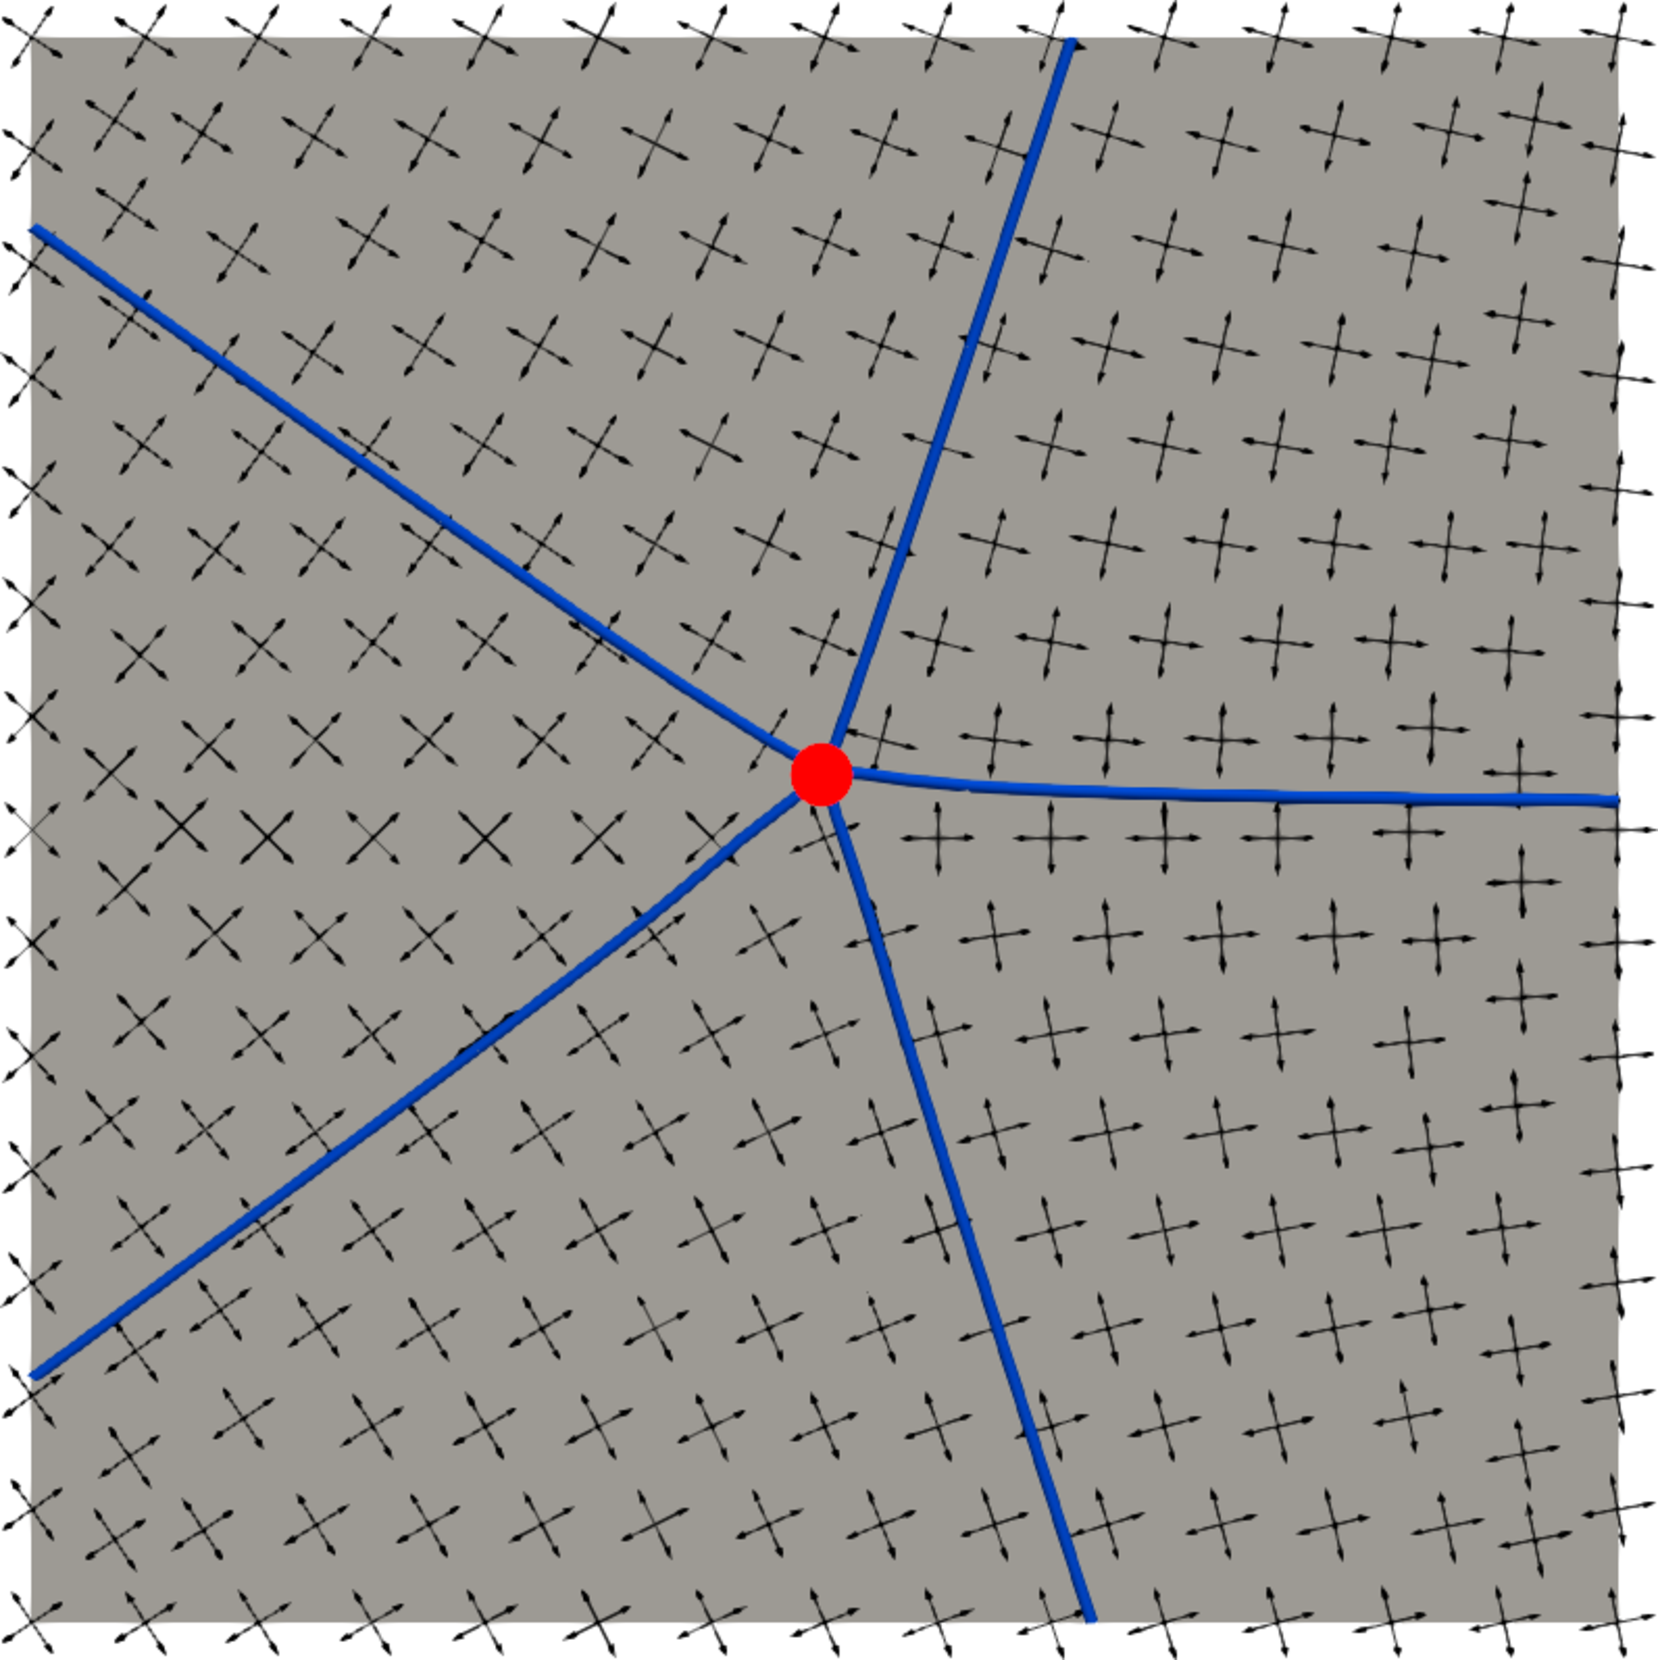
\includegraphics[scale=0.282]{images/sepa_5.pdf}
  \hfill
  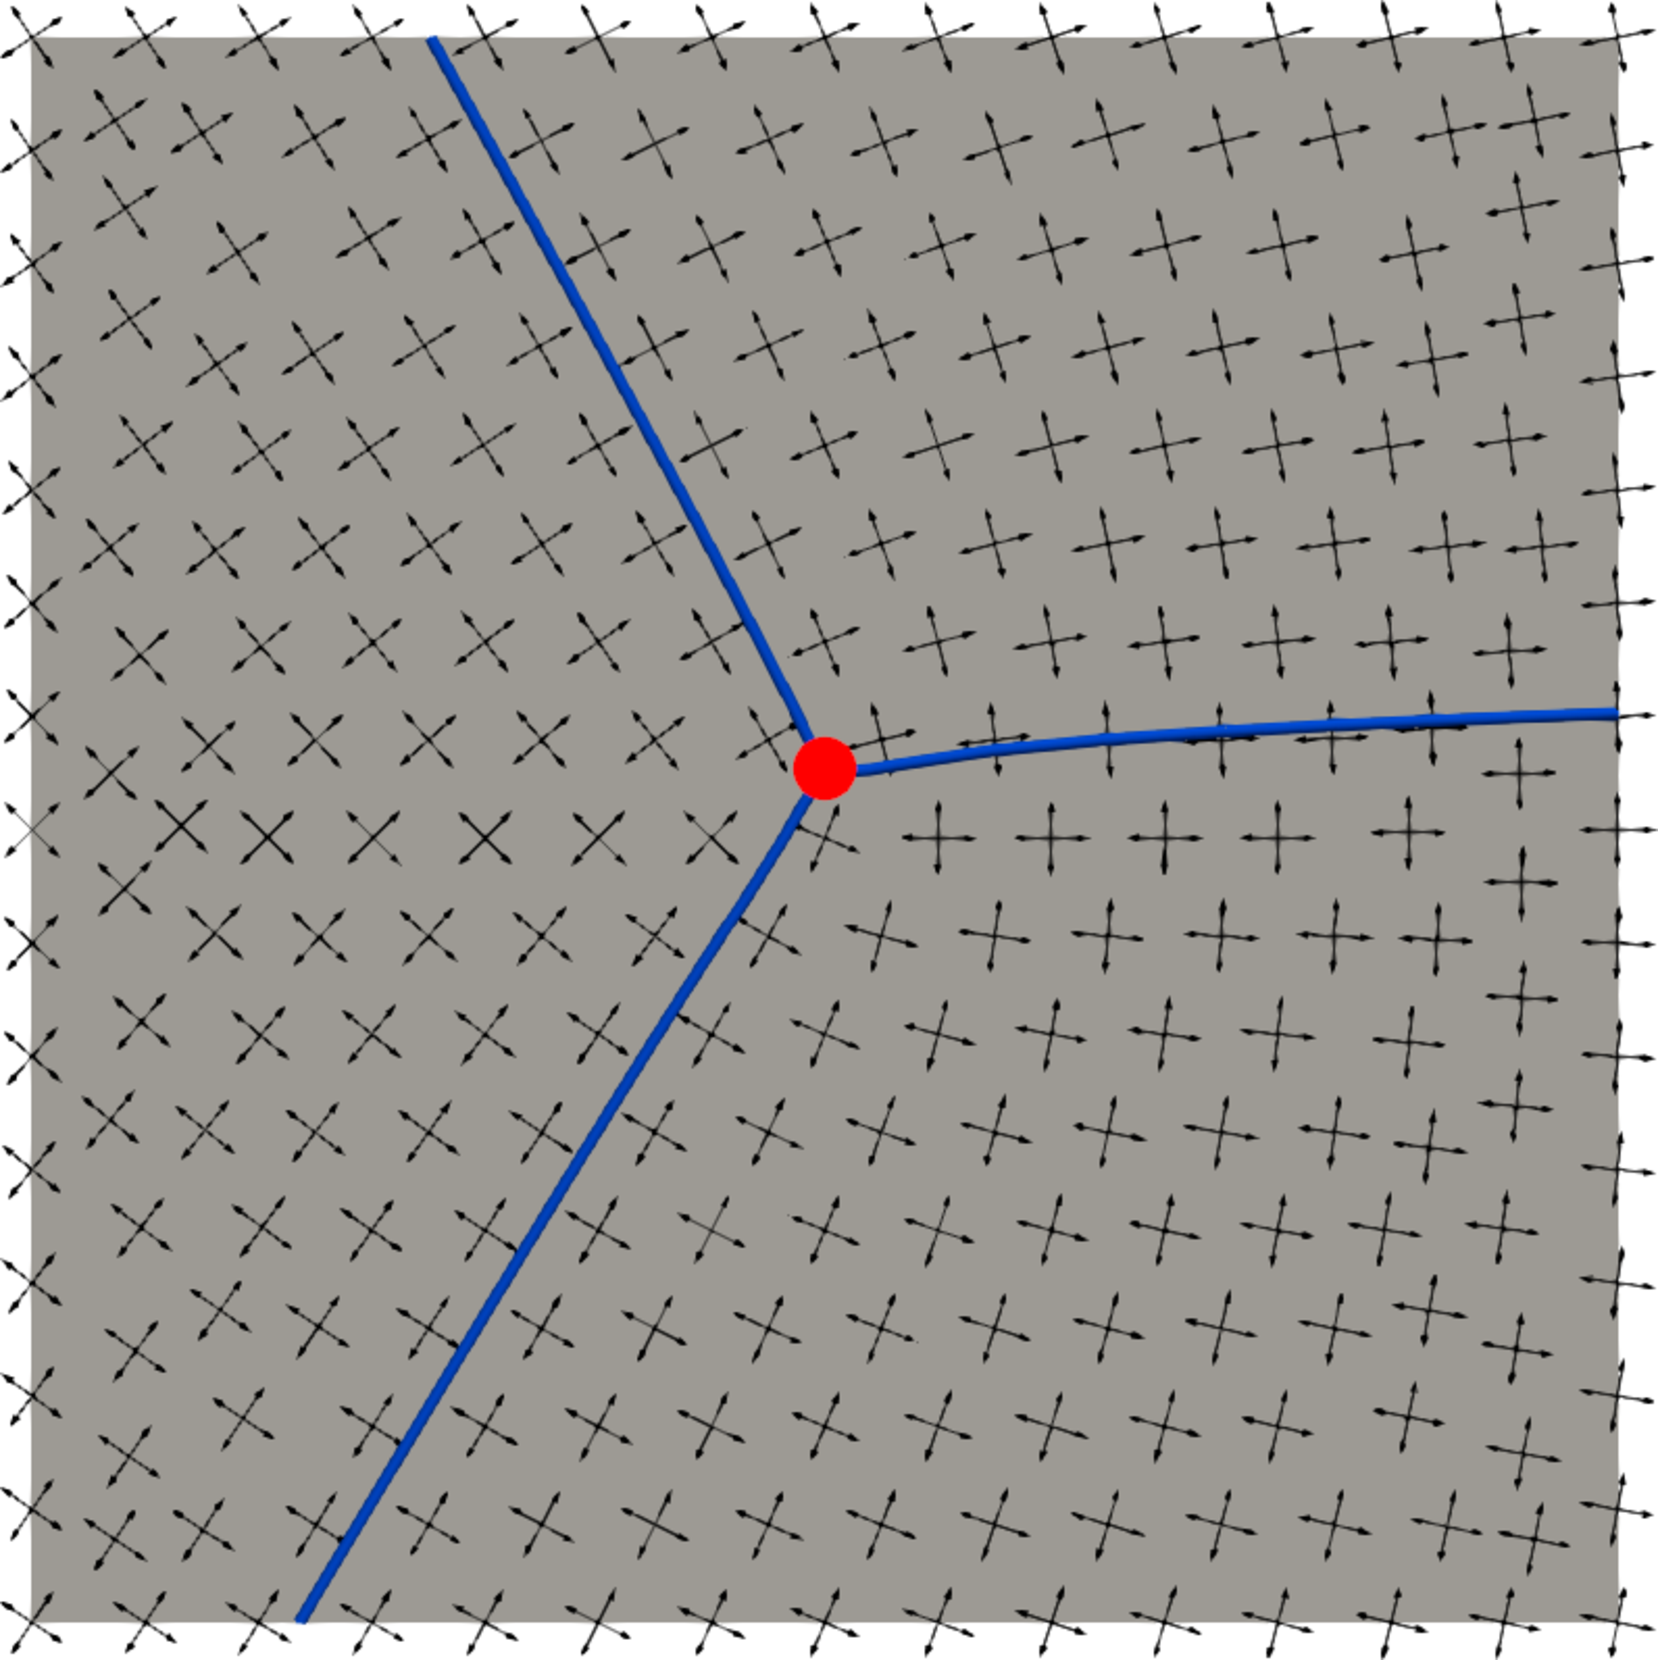
\includegraphics[scale=0.282]{images/sepa_3.pdf}
  \caption{Gauche: Illustration des séparatrices émanant de points singuliers d'indice $-1/4$ (à gauche) et d'indice $1/4$ (à droite).}
  \label{fig:separatrice_illustration}
\end{figure}

\begin{proposition}
\label{prop:loveprop}
Considérons un secteur tel que décrit ci-dessus. Lorsqu'il est traité comme une singularité de bord du secteur, le point $p$ a un indice de $1/4$.
\end{proposition}

\begin{proof}
Supposons que le secteur soit défini par deux séparatrices avec des directions initiales $\overrightarrow{p\gamma(t_i)}$ et $\overrightarrow{p\gamma(t_{i+1})}$, qui sont alignées avec la frontière du secteur. Soit $C$, la paramétrisation de la courbe définie par $p\gamma(t_i)$, $p\gamma(t_{i+1})$ et la partie de $\gamma$ coincé dans le secteur. L'indice de $p$ est alors donné par:
\begin{eqnarray*}
id^\partial_{\bar{u}}(p)&=&\frac{1}{2\pi}\left[\pi-\hat{p}+\lim\limits_{s\rightarrow 0}\int_{s-t_i}^{s-t_{i+1}}d\theta_{\bar{u}}^\gamma\right]\\
&=&\frac{1}{2\pi}\left[\pi-\hat{p}+\left(\hat{p}+\lim\limits_{s\rightarrow 0}\int_{s-t_i}^{s-t_{i+1}}dW_p^\gamma\right)\right]\\
&=&\frac{1}{2\pi}\left[\pi-\frac{\pi}{2}\right]\\
id^\partial_{\bar{u}}(p)&=&\frac{1}{4}.
\end{eqnarray*}
\end{proof}

De manière analogue à ce qui est fait dans \cite{viertel2019approach}, la proposition \ref{prop:loveprop} implique que l'apparence de chaque coin d'un secteur est celle d'un angle droit par rapport au champ de croix.

\begin{comment}
\[\]
commentaires sur les secteurs\\
on retrouve ici la notion de valence évoqué dans l'introduction.
un point sera dit régulier si Ns= autrement dit si id=
reprendre les dessin sur l'illustration des index, tracer les sepatrices pour visulaiser ce qu'est un secteur.
\end{comment}


\section{Méthode de partitionnement à partir d'un champ de croix}

Nous abordons maintenant le cœur de ce chapitre en présentant la méthode de partitionnement de domaine basée sur les champs de croix. Dans un premier temps, nous exposons l'algorithme de partitionnement ainsi que les différentes conditions requises sur le champ de croix, garantissant ainsi que le partitionnement obtenu résulte en un maillage quadrilatéral du domaine de départ. Par la suite, nous analysons en détail les différents algorithmes présentés et fournissons des résultats permettant de garantir leur bon fonctionnement.

\subsection{Principe de la méthode}
\label{subsec:principe_methode}

Considérons un domaine $\Omega$ borné et fermé dans $\mathbb{R}^2$ possédant une frontière $\partial\Omega$ régulière par morceaux. L'algorithme suivant permet de partitionner ce domaine en régions distincts.

\vspace{0.5cm}
\RestyleAlgo{ruled}
\begin{algorithm}[H]
\label{alg:algo_main}
\renewcommand{\algorithmcfname}{Algorithme}%
\SetAlgoLined
\Entrees{$\Omega$ un domaine borné et fermé; Un champ de croix presque-$\mathcal{C}^1$ défini sur $\Omega$ est tel que l'indice des points dans ce champ est égal à $k/4$, où $k\in\mathbb{Z}$ et $k\leq 1$.}
\Sortie{Partition de $\Omega$ en ensembles de régions.}
\vspace{0.2cm}
1.\quad Identification des points singuliers du champ de croix,\\\vspace{0.2cm}
2.\quad Détermination du nombre de séparatrices pour chaque point singulier,\\\vspace{0.2cm}
3.\quad Intégration des lignes de champ pour construire les séparatrices,\\\vspace{0.2cm}
4.\quad Identification des régions.\\\vspace{0.2cm}
\caption{Algorithme de partitionnement}
\end{algorithm}
\vspace{0.5cm}

\begin{enumerate}
\item \textbf{Identification des points singuliers :} l'algorithme commence par identifier les points singuliers dans le champ de croix fourni. Ces points singuliers jouent un rôle critique dans la détermination de la structure du maillage. Ils correspondent à des points $p\in\Omega$, tels que $\bar{u}(p)=0$ (voir la première image de la figure \ref{fig:demi_disc_align_first}).\\
\item \textbf{Détermination du nombre de séparatrices pour chaque point singulier :}
le nombre de lignes de champ provenant de chaque point singulier est directement lié à l'indice du point dans le champ de croix Plus précisément, si $p\in\Omega\backslash\partial\Omega$, alors $N_s(p) = 4 - 4id_{\bar{u}}(p)$, tandis que si $p\in\partial\Omega$, alors $N_s(p) = 4 - 4id_{\bar{u}}^\partial(p)$ où $N_s(p)$ représente le nombre de séparatrices associé au point $p$ (voir les propositions \ref{prop:align_sepa_voisinnage} et \ref{prop:align_sepa_voisinnage_bord}).\\
\item \textbf{Construction des séparatrices :} les séparatrices de chaque point singulier sont initialisées selon la proposition $\ref{prop:stream_from_interior_sing}$ puis les lignes de champs sont intégrées à travers le domaine en utilisant l'équation \eqref{eqn:streamline} (voir la deuxième image de la figure \ref{fig:demi_disc_align_second}). Les directions initiales de ces séparatrices sont déterminées en cherchant des directions alignées avec le champ de croix dans le voisinnage du points singuliers  (voir les propositions \ref{prop:align_sepa_voisinnage} et \ref{prop:align_sepa_voisinnage_bord}).\\
\item \textbf{Identification des régions :} si aucune des séparatrices ne converge vers un cycle limite alors l'algorithme à converger et les séparatrices construites partitionnent avec le bord du domaine en un ensemble fini de régions.\\
\end{enumerate}

On considère que l'algorithme
\ref{alg:algo_main} a convergé si les constructions de séparatrices ne convergent pas vers des cycles limites. Examinons à présent les conditions sur le champ de croix qui permettent, à partir de l'algorithme présenté ci-dessus, d'obtenir un maillage quadrilatéral d'un domaine donné.

\subsubsection*{Construction à partir d'un champ de croix aligné sur le bord de $\Omega$}

Lorsque le champ de croix est aligné par rapport à $\partial\Omega$, on peut montrer (voir le Théorème \ref{thm:theorem1}) que le partionnement issue de l'Algorithme \ref{alg:algo_main} est constitué de régions ayant 4 côtés. Chacune de ces régions peut alors être maillée en quadrilatères en utilisant une méthode de paramétrisation comme l'interpolation transfinie. Par exemple, sur la figure \ref{fig:demi_disc_align}, nous considérons un champ de croix aligné avec le bord du domaine (voir figure \ref{fig:demi_disc_align_first}). Ce champ comporte deux points singuliers intérieurs d'indice $1/4$ chacun, ainsi que deux points singuliers de bord d'indice $1/4$ chacun. L'application de l'algorithme de partitionnement permet d'obtenir le partitionnement présenté sur la figure \ref{fig:demi_disc_align_second}. Chaque région est ensuite maillé sur la figure \ref{fig:demi_disc_align_third}.

\begin{figure}[!h]
\centering
\begin{subfigure}{0.64\textwidth}
    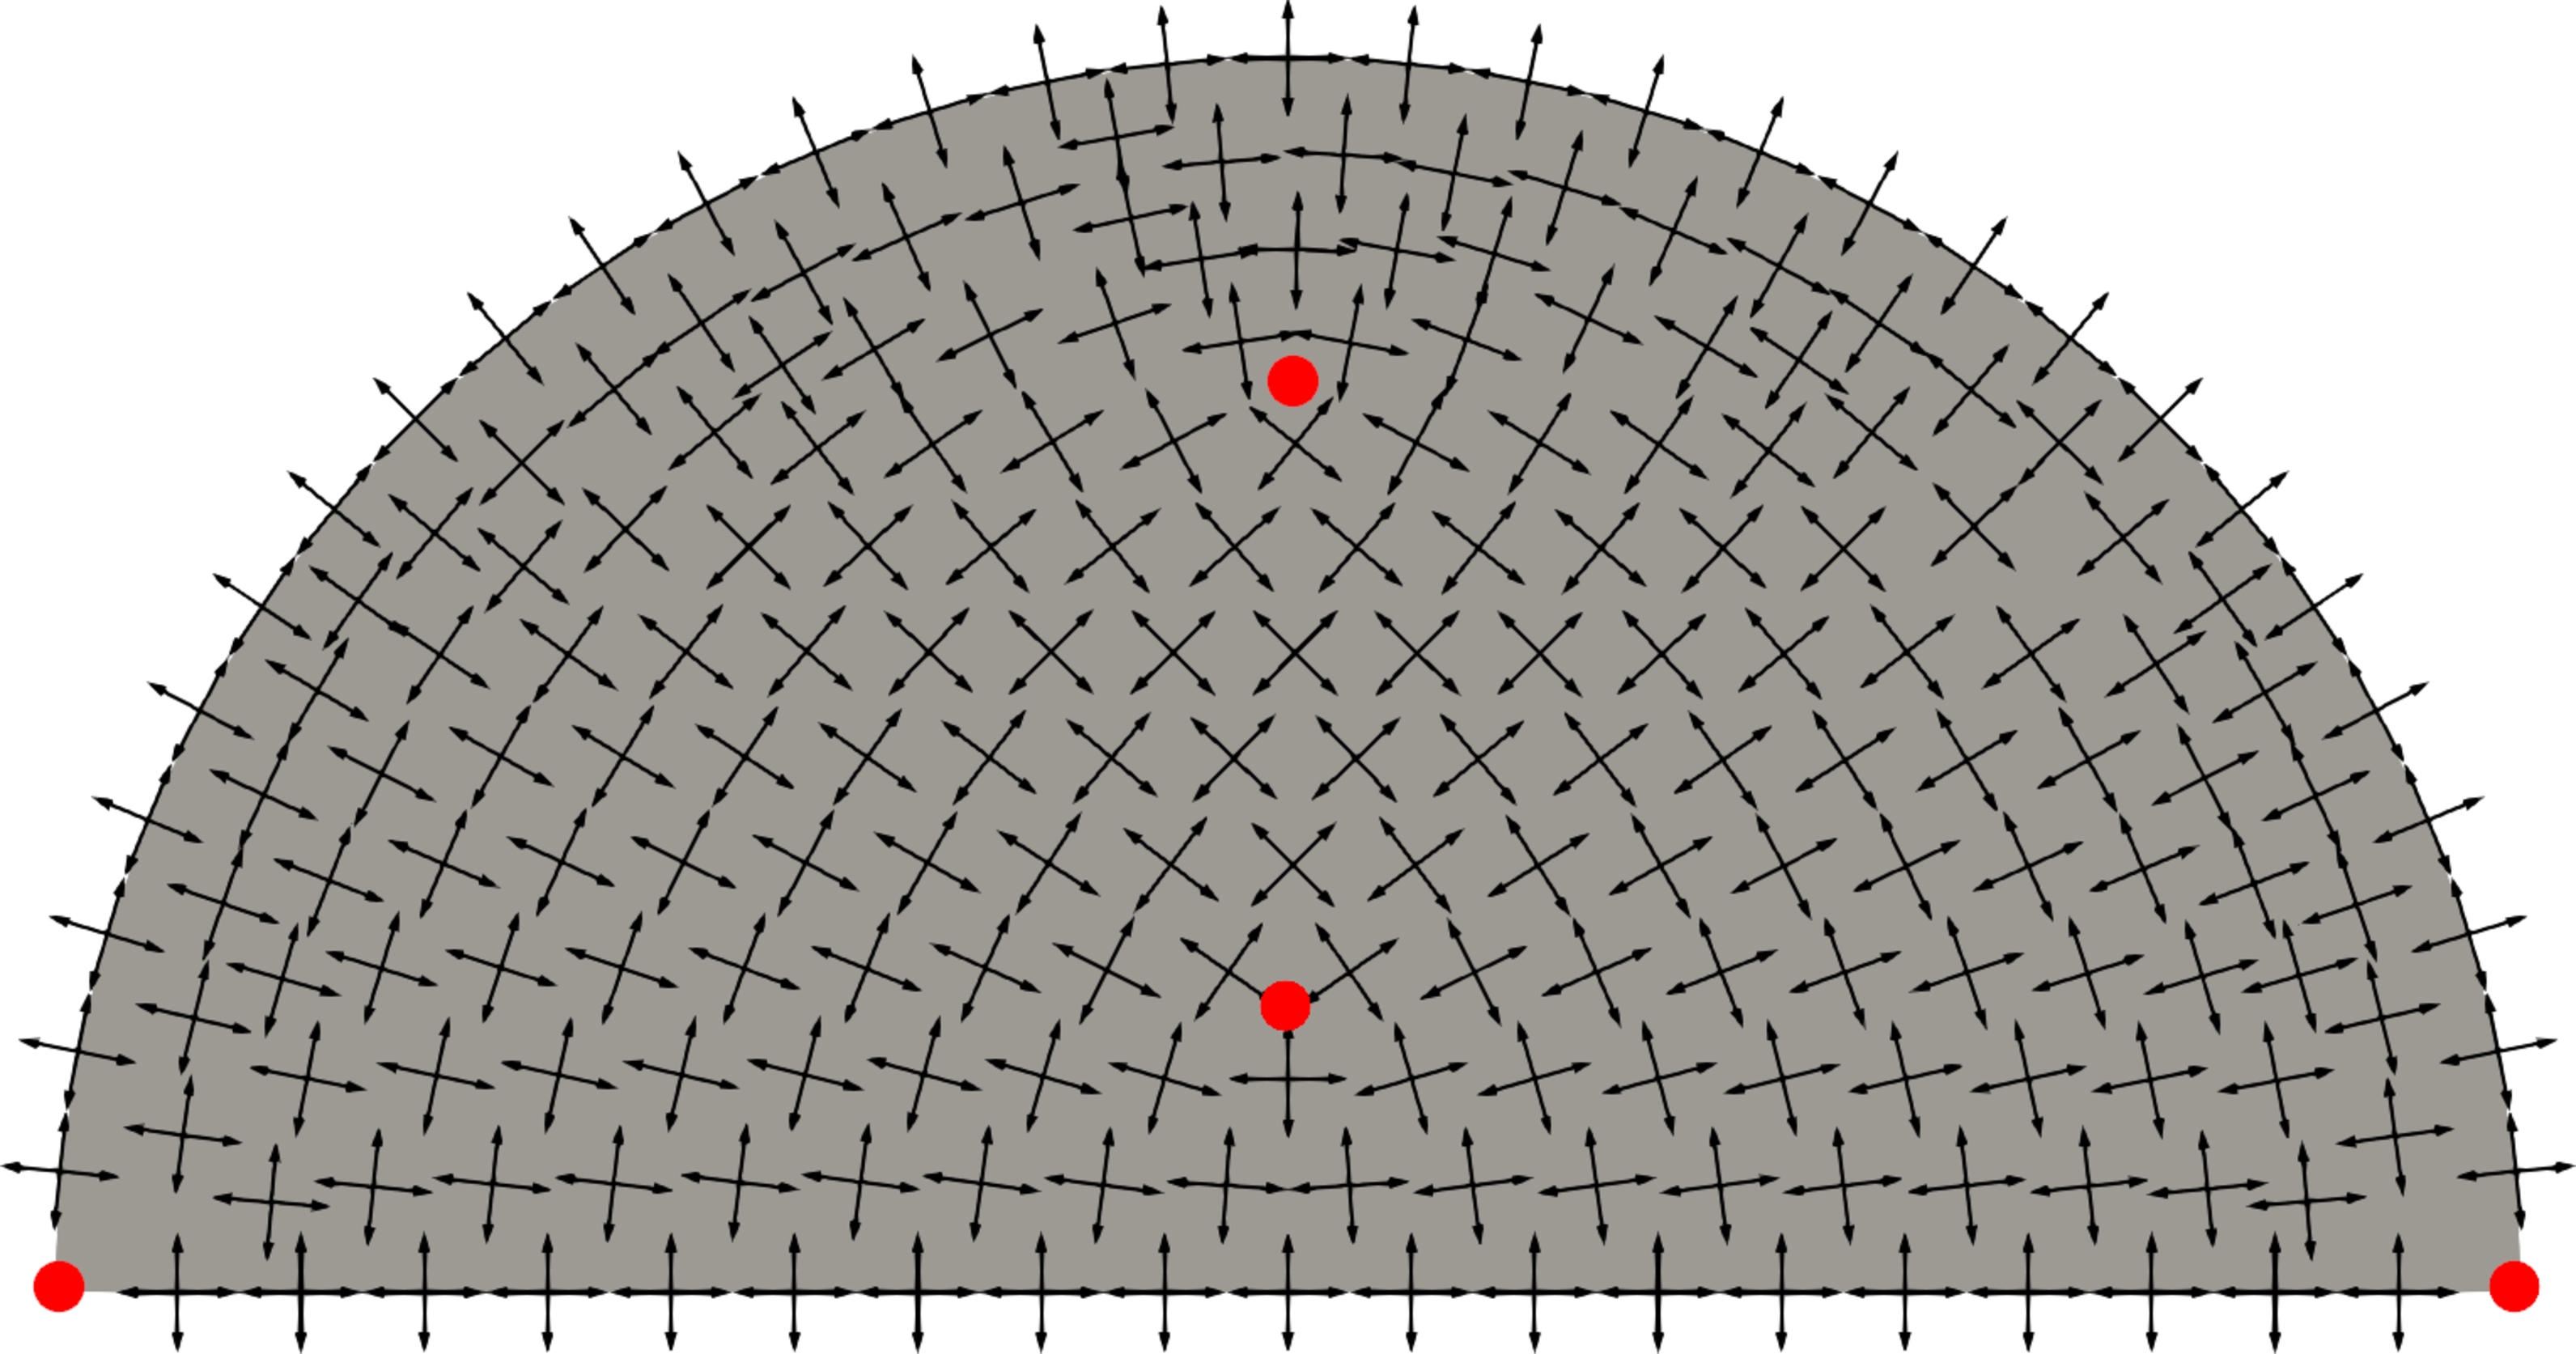
\includegraphics[width=\textwidth]{images/demi_disc_align_first.pdf}
    \caption{Champ de croix aligné sur le bord du domaine (points singuliers en rouge).}
    \label{fig:demi_disc_align_first}
\end{subfigure}
\\[3ex]
\begin{subfigure}{0.64\textwidth}
    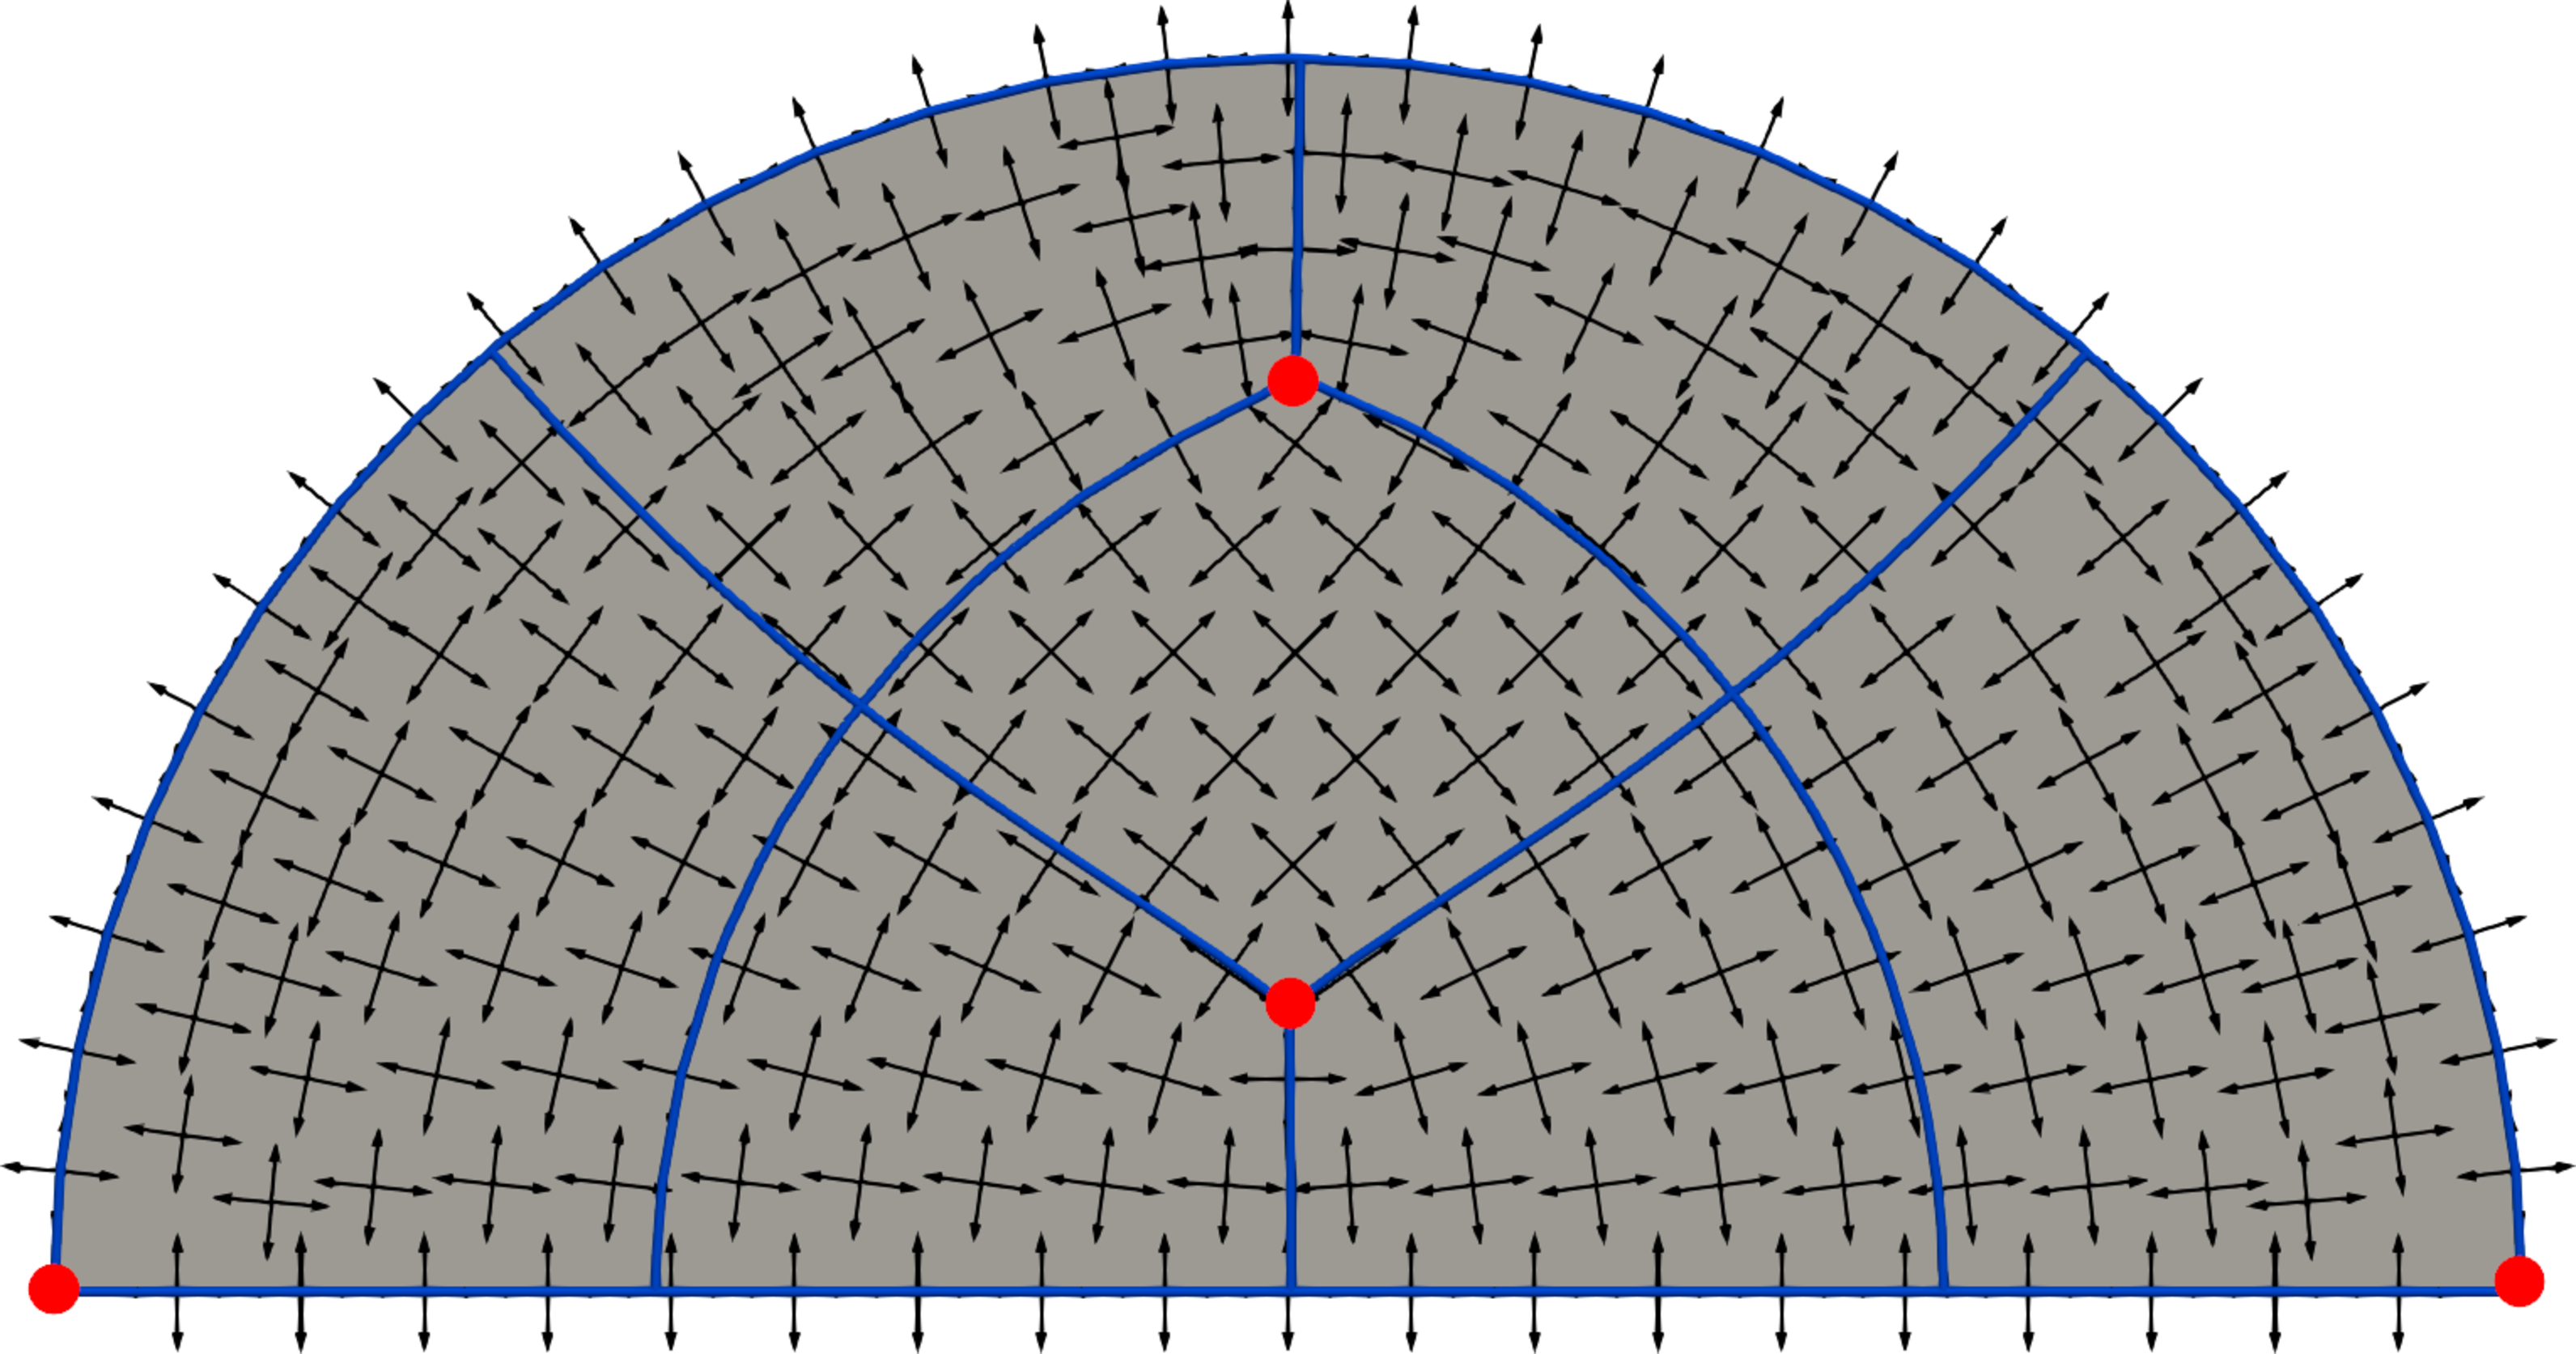
\includegraphics[width=\textwidth]{images/demi_disc_align_second.pdf}
    \caption{Partitionnement du Domaine.}
    \label{fig:demi_disc_align_second}
\end{subfigure}
\\[3ex]
\begin{subfigure}{0.64\textwidth}
    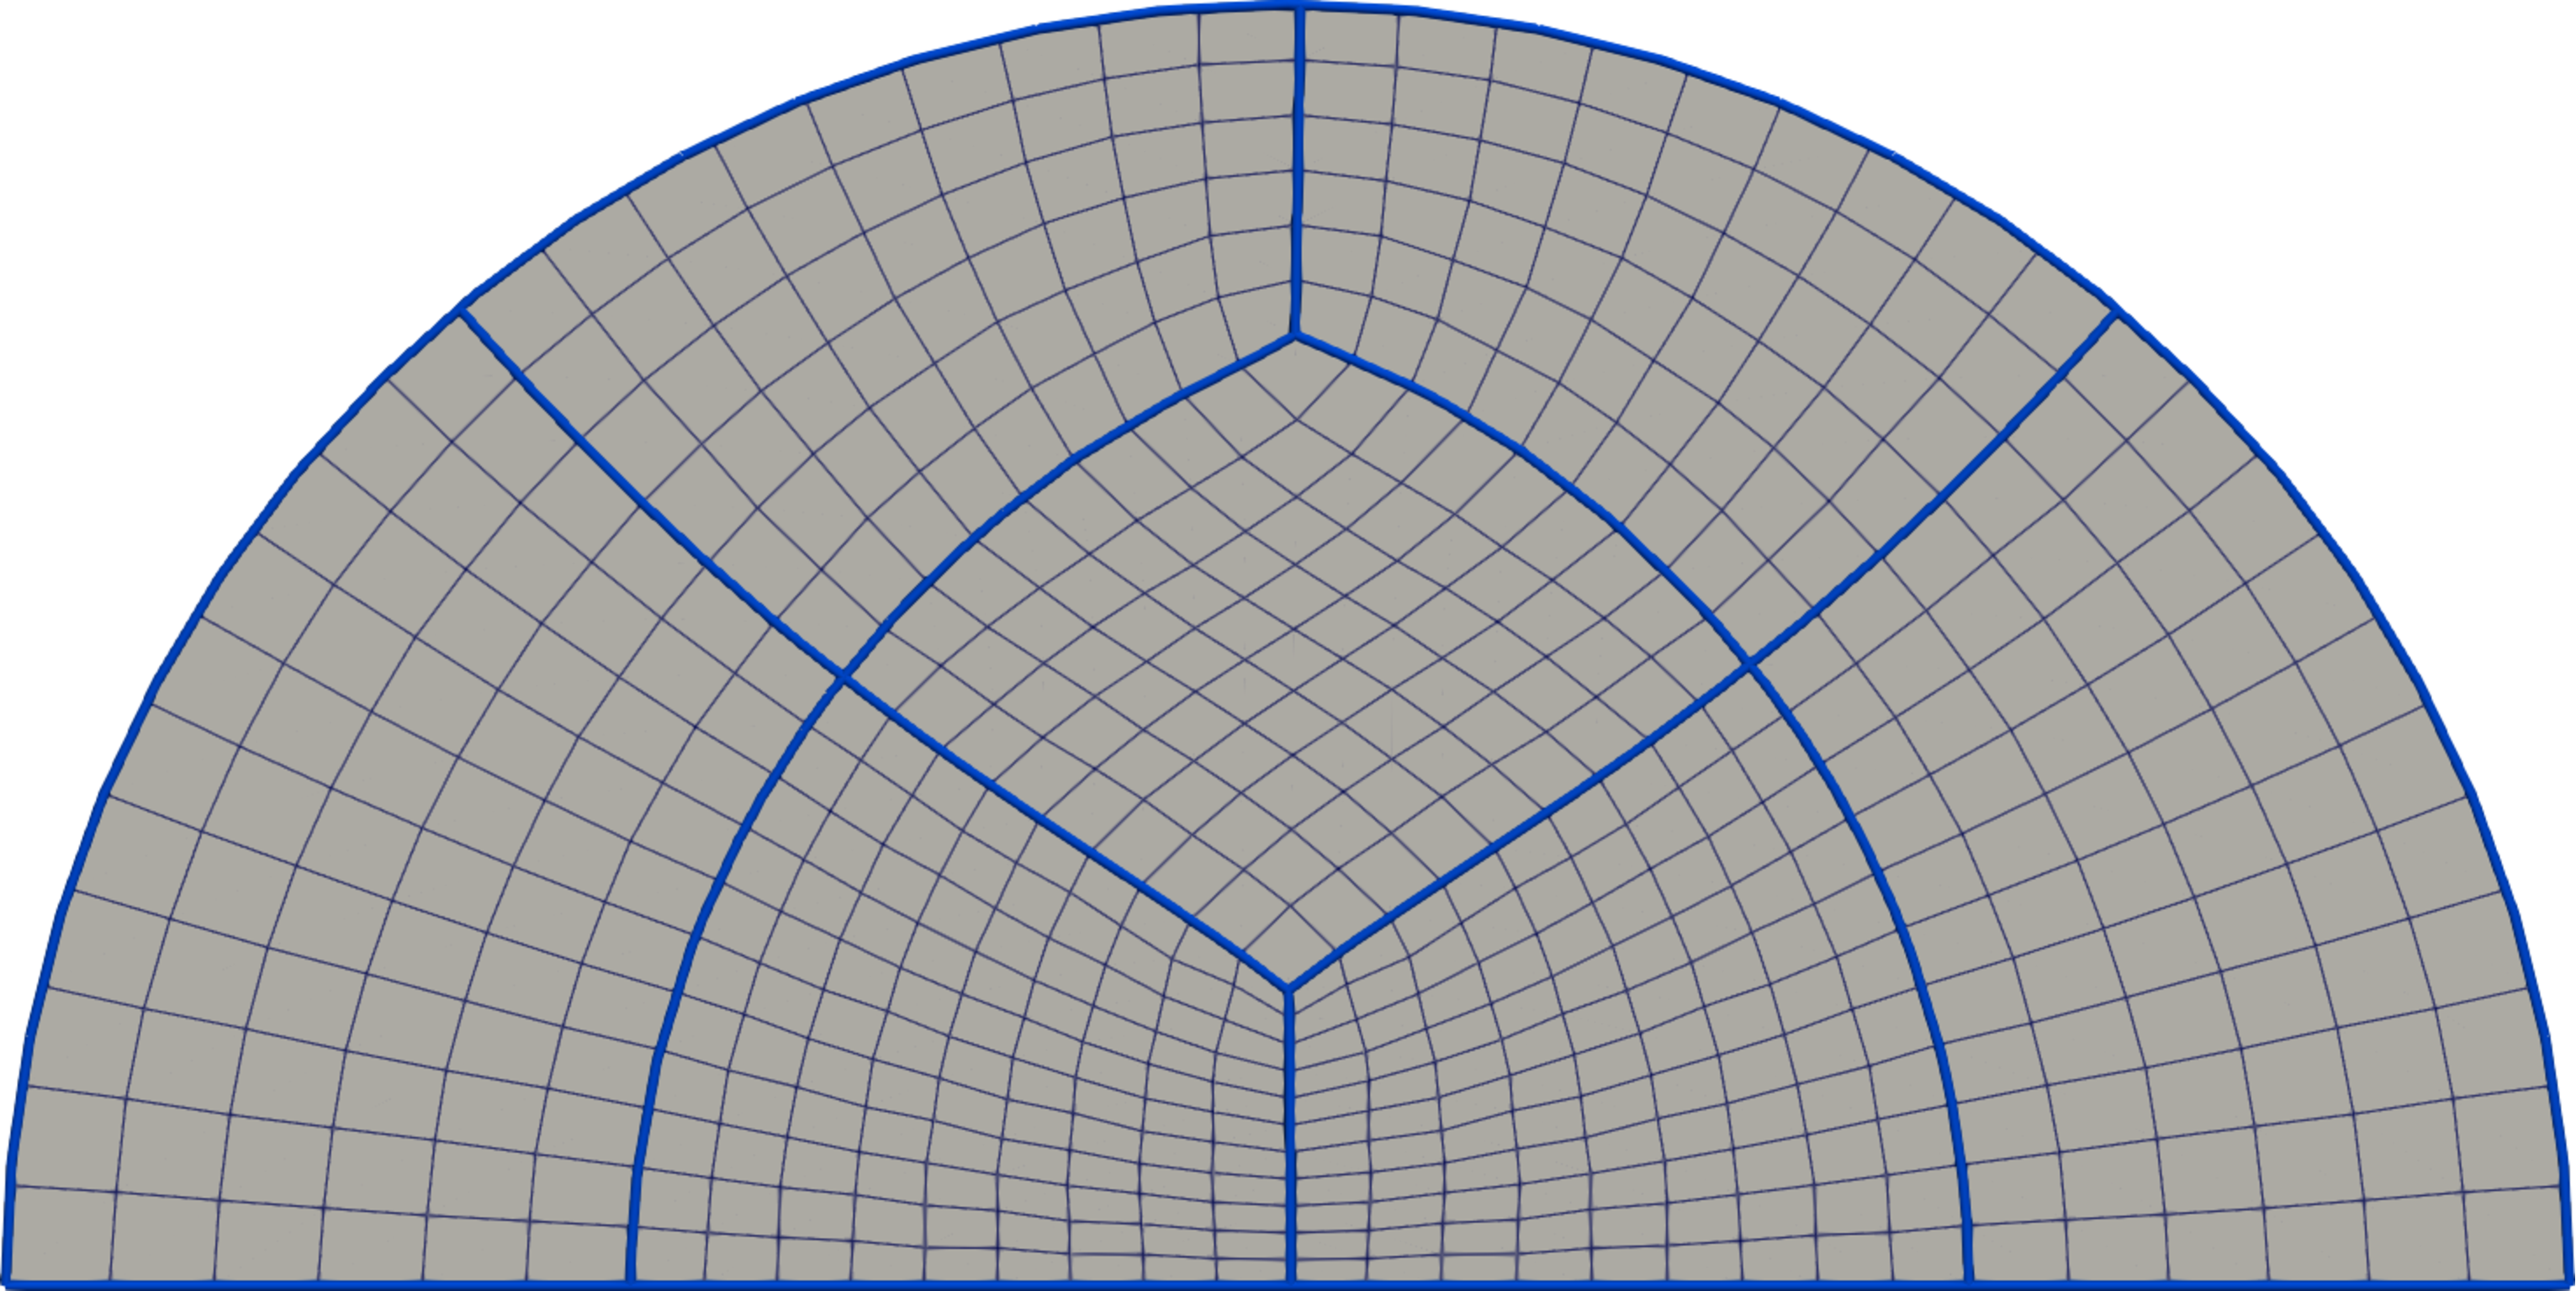
\includegraphics[width=\textwidth]{images/demi_disc_align_third.pdf}
    \caption{Maillage quadilatéral du domaine.}
    \label{fig:demi_disc_align_third}
\end{subfigure}

\caption{Maillage quadrilatéral d'un domaine à partir d'un champ de croix aligné sur le bord du domaine.}
\label{fig:demi_disc_align}
\end{figure}

\subsubsection*{Construction à partir d'un champ de croix non-aligné sur le bord de $\Omega$}

Comme indiqué dans l'introduction, notre objectif est de permettre l'utilisation de différents types de champs de croix. Par exemple, un champ de croix peut être construit en prenant le quart de l'angle des vecteurs du champ de gradient d'un mode propre particulier du Laplacien (voir la figure \ref{fig:demiDisc_valProp}). La même construction peut être appliquée aux lignes de niveau.

\begin{figure}[!h]
\centering
\begin{subfigure}{0.65\textwidth}
    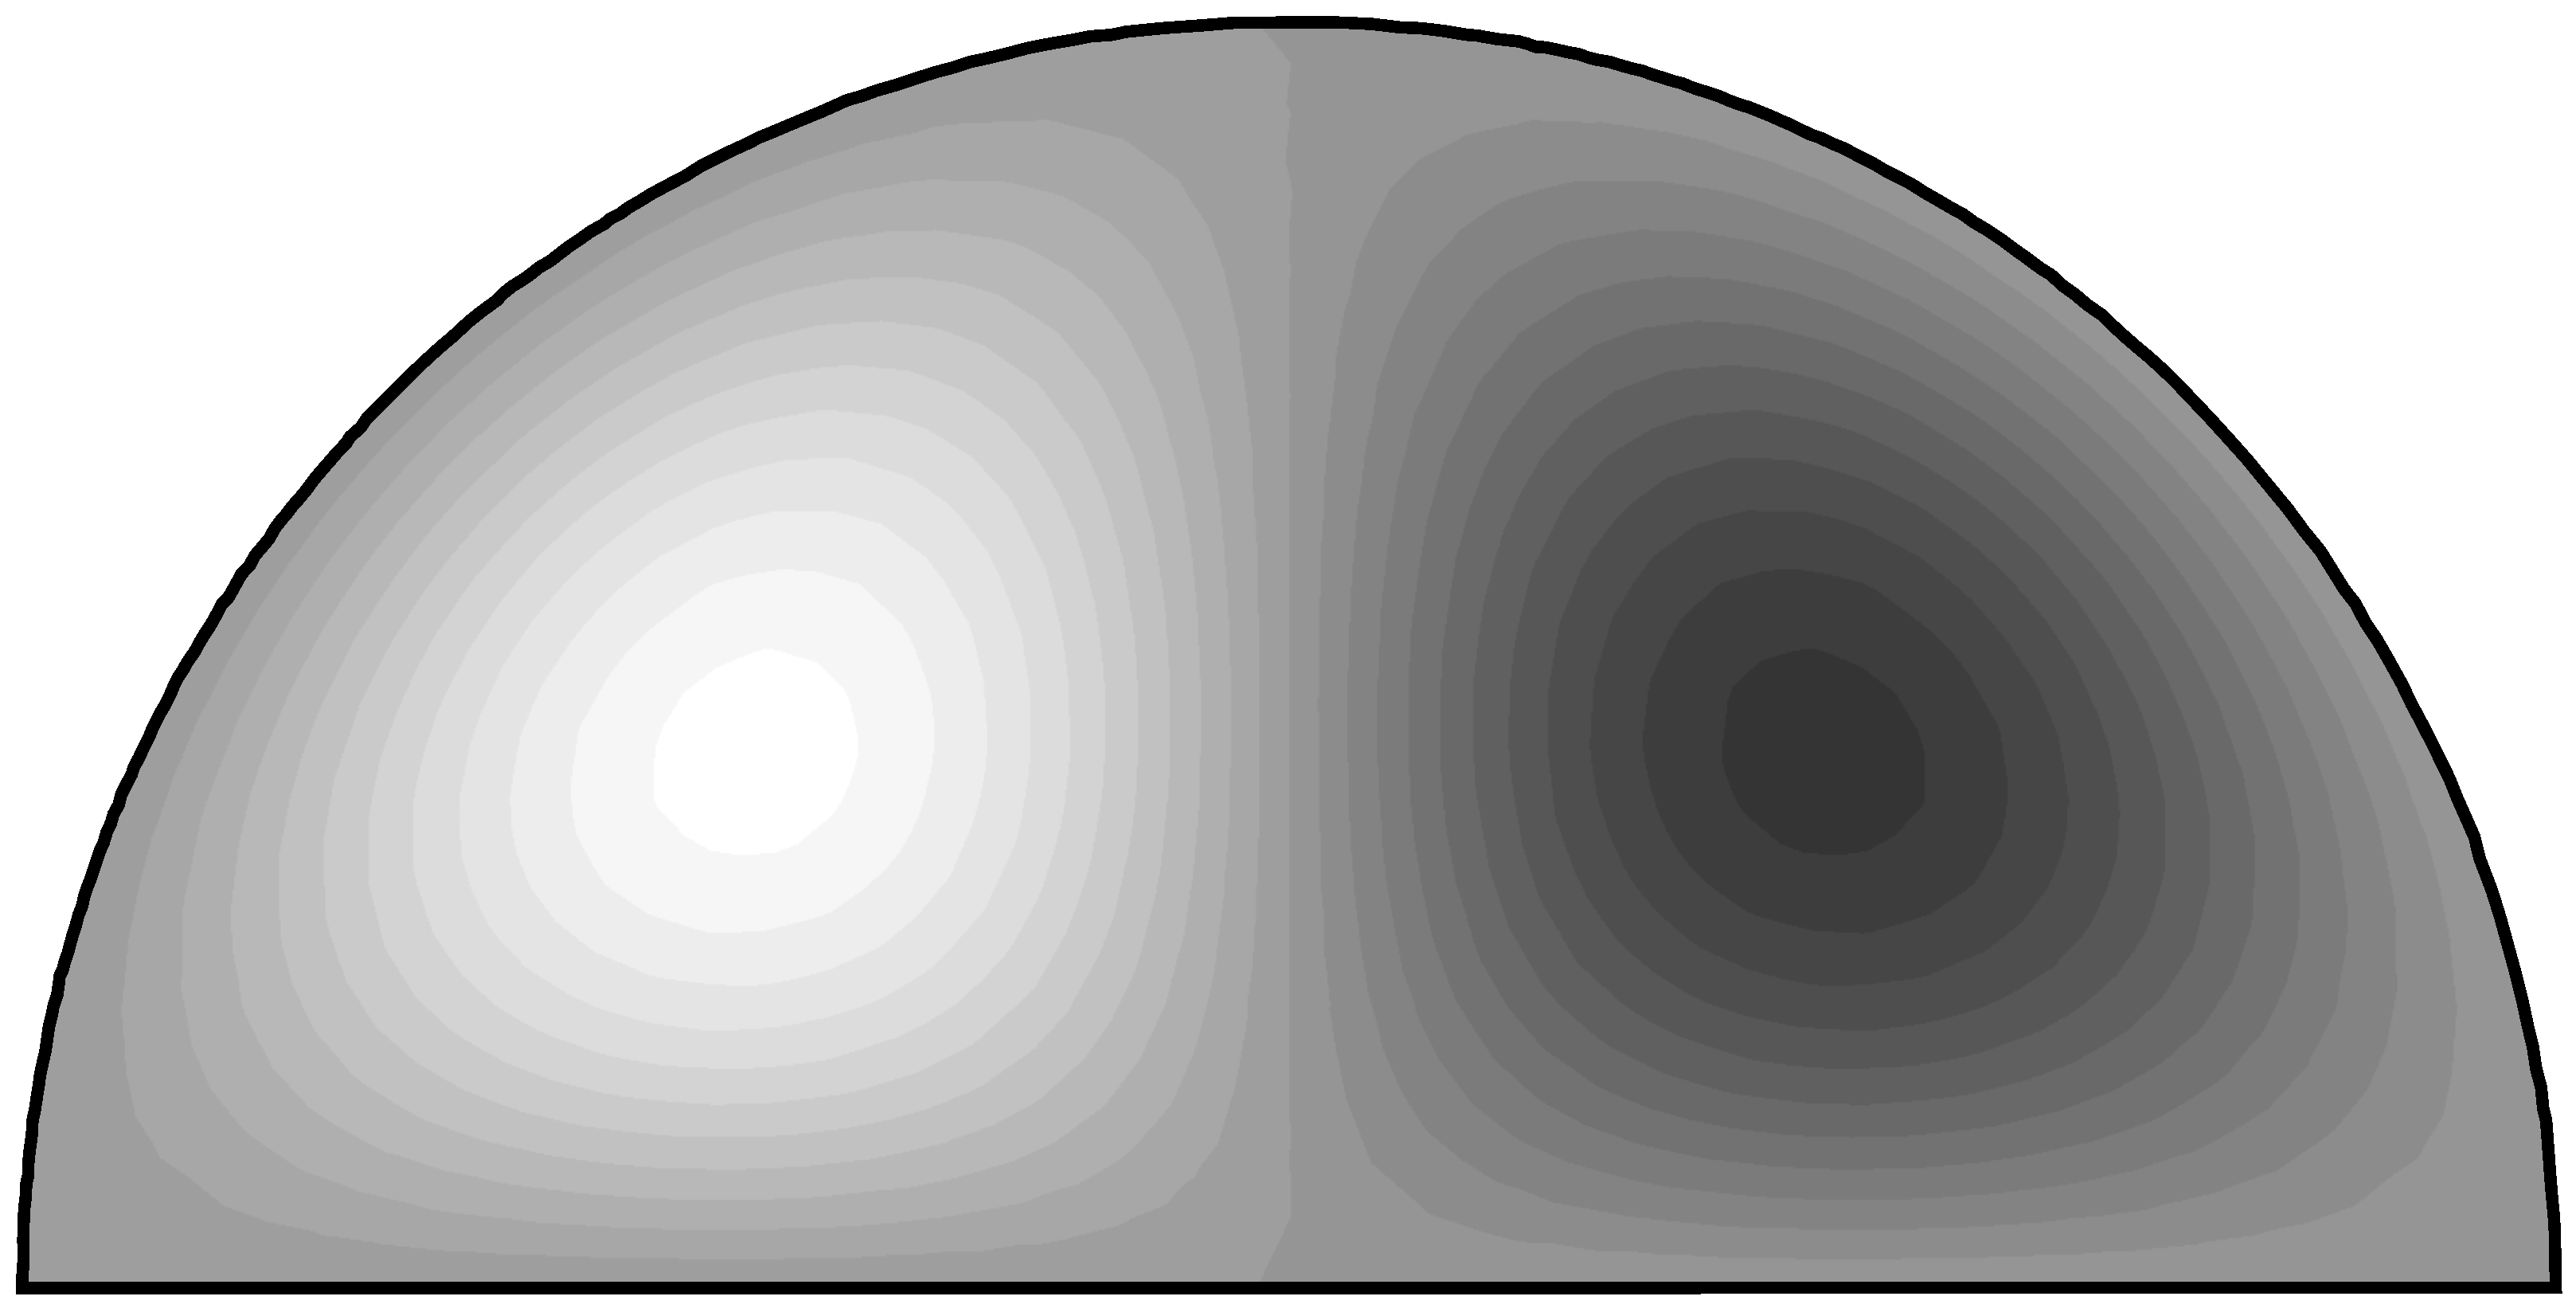
\includegraphics[width=\textwidth]{images/demiDiscValProp.eps}
    \caption{Un mode propre du Laplacien sur le demi disque.}
    \label{fig:demiDiscValPropSheet_first}
\end{subfigure}
\\[3ex]
\begin{subfigure}{0.75\textwidth}
    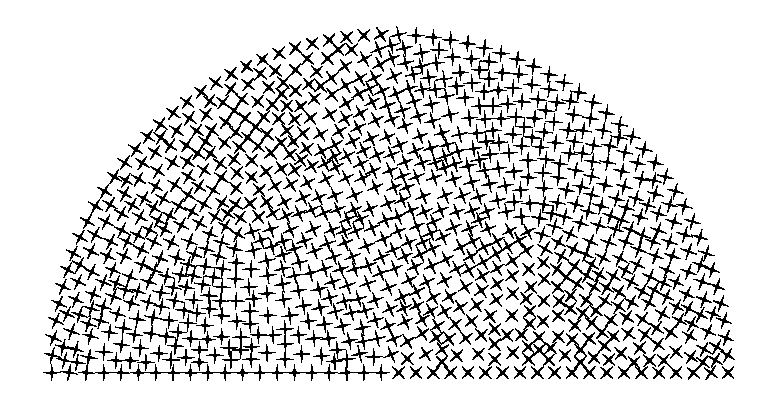
\includegraphics[width=\textwidth]{images/demiDiscValPropSheet.eps}
    \caption{Champ de croix construit à partir du mode propre.}
    \label{fig:demiDiscValPropSheet_second}
\end{subfigure}

\caption{Génération d'un champ de croix à partir d'un mode propre du Laplacien.}
\label{fig:demiDisc_valProp}
\end{figure}

On observe que les extrémas du mode propre coïncident avec les points singuliers correspondants du champ de croix construit. Ces points singuliers sont donc approximativement à une distance égale les uns des autres et de la frontière. Nous visons à conserver cette caractéristique du champ de croix dans le maillage final, ce qui aboutira à une distribution plus uniforme des éléments du maillage. Plus généralement, notre motivation est de choisir d'autres types de champs de croix de manière à ce que le maillage quadrilatéral résultant hérite de certaines propriétés du champ de croix initialement choisi, notamment la position et la nature des points singuliers.

Cependant, lorsqu'un champ de croix, tel que décrit ci-dessus, est utilisé pour diviser le domaine (via l'Algorithme \ref{alg:algo_main}), on constate que certaines régions s'éloignent de la forme quadrilatérale habituelle, comme illustré dans la figure \ref{fig:demiDisc_valProp_mauvaix_decoup}. Cette déviation est due au fait que le champ de croix n'est pas aligné correctement avec les frontières du domaine. Par conséquent, certaines partitions ne possèdent pas quatre côtés.

\begin{figure}[!h]
\centering
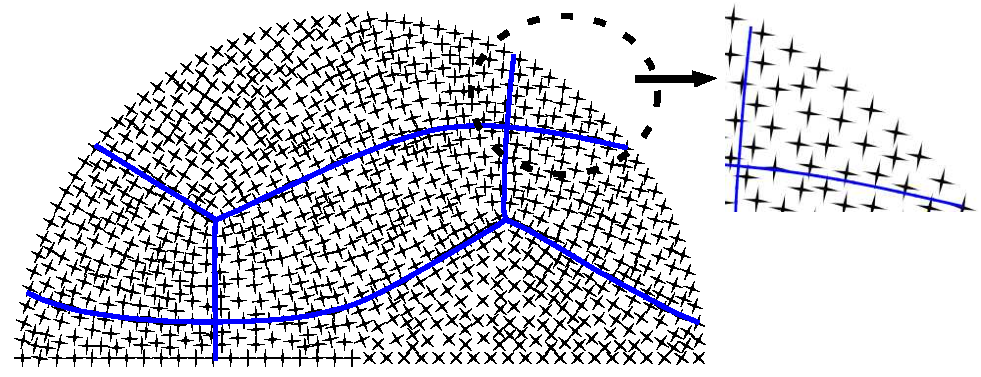
\includegraphics[scale=0.8]{images/gagaga.pdf}
\caption{Découpage invalide obtenue à partir du champ de croix de la figure \ref{fig:demiDisc_valProp}.}
\label{fig:demiDisc_valProp_mauvaix_decoup}
\end{figure}


Pour remédier à cette difficulté, nous introduisons une opération sur le champ de croix appelée \emph{opération d'alignement}. L'objectif est d'ajuster le champ de croix pour qu'il soit aligné avec la frontière du domaine. Pour ce faire, nous cherchons un champ scalaire avec une certaine régularité tel que la rotation du champ de croix initial par rapport à ce champ scalaire donne un nouveau champ de croix aligné avec les frontières du domaine tout en préservant certaines propriétés du champ de croix initial. Dans la suite, nous détaillerons cette opération tout en désignant par \emph{champ d'alignement} le champ scalaire décrit ci-dessus. Pour simplifier la présentation, nous mettons en place l'opération d'alignement dans un premier temps sur un domaine simplement connexe avant de l'étendre aux domaines non-simplement connexes.

\paragraph{Domaines simplement connexes:}
On suppose $\Omega$ simplement connexe. Soit $\bar{u}$ un champ de croix presque-$\mathcal{C}^1$ défini sur $\Omega$ et non-nécessairement aligné sur le bord de $\Omega$ tel que $0<Card(\mathcal{S}_{\bar{u}})<\infty$ et pour tout point $p\in\mathcal{S}_{\bar{u}}\backslash\partial\Omega$, $id_{\bar{u}}(p)=k/4$, avec $k\in\mathbb{Z}$ et $k\leq 1$. A priori, une façon simple de réaliser l'opération d'alignement serait de calculer la différence angulaire entre le champ de croix $\bar{u}$ et le champ de croix normal $\bar{n}$ puis de diffuser continûment cette différence angulaire à l'intérieur du domaine. En faisant cela on construirait un champ scalaire régulier sur tout le domaine tel que la rotation du champ de croix par rapport à ce champ scalaire donnerait un champ de croix aligné sur le bord du domaine et n'affectant pas les points singuliers du champ de croix initial en vertu de la proposition $\ref{prop:cont1}$. Un bon candidat pour la diffusion serait alors l'équation de Laplace donné par:
\begin{equation}
\left\{
\begin{array}{lcll}
\Delta\phi &=& 0 &\mbox{ dans }\Omega,\\[0.5cm]
\phi(p) &=& \widehat{(\bar{n}(p); \bar{u}(p))}=\theta_{\bar{n}}(p)-\theta_{\bar{u}}(p)&\mbox{ sur } \partial\Omega,
\end{array}
\right.
\label{eqn:first_phi_computation}
\end{equation}
où $\widehat{(\bar{n}(p); \bar{u}(p))}$ représente l'angle entre $\bar{n}(p)$ et $\bar{u}(p)$. En définissant $\bar{v}:=\mathbf{R}(\phi)\bar{u}$, il est évident que $\bar{v}=\bar{n}$ sur $\partial\Omega$, impliquant ainsi que $\bar{v}$ est aligné avec $\partial\Omega$. De plus, grâce à la proposition \ref{prop:relation_u_Rthetau}, nous savons que pour tout $p\in\Omega\backslash\partial\Omega$, $id_{\bar{v}}(p)=id_{\bar{u}}(p)$. Par conséquent, si l'algorithme de partitionnement \ref{alg:algo_main} converge lorsqu'il est appliqué à $\bar{v}$, nous obtenons un partitionnement de $\Omega$ en régions à quatre côtés (voir le Théorème \ref{thm:theorem1}). Cependant, une question demeure en suspens : quelle est la valeur des indices des points situés sur le bord de $\Omega$ dans le champ de croix $\bar{v}$? Cela va dépendre de la représentation angulaire choisie pour $\phi$ à un multiple de $\pi/2$ près dans la condition de bord de l'équation \eqref{eqn:first_phi_computation}.

\begin{figure}[!h]
\centering
\begin{subfigure}{0.65\textwidth}
    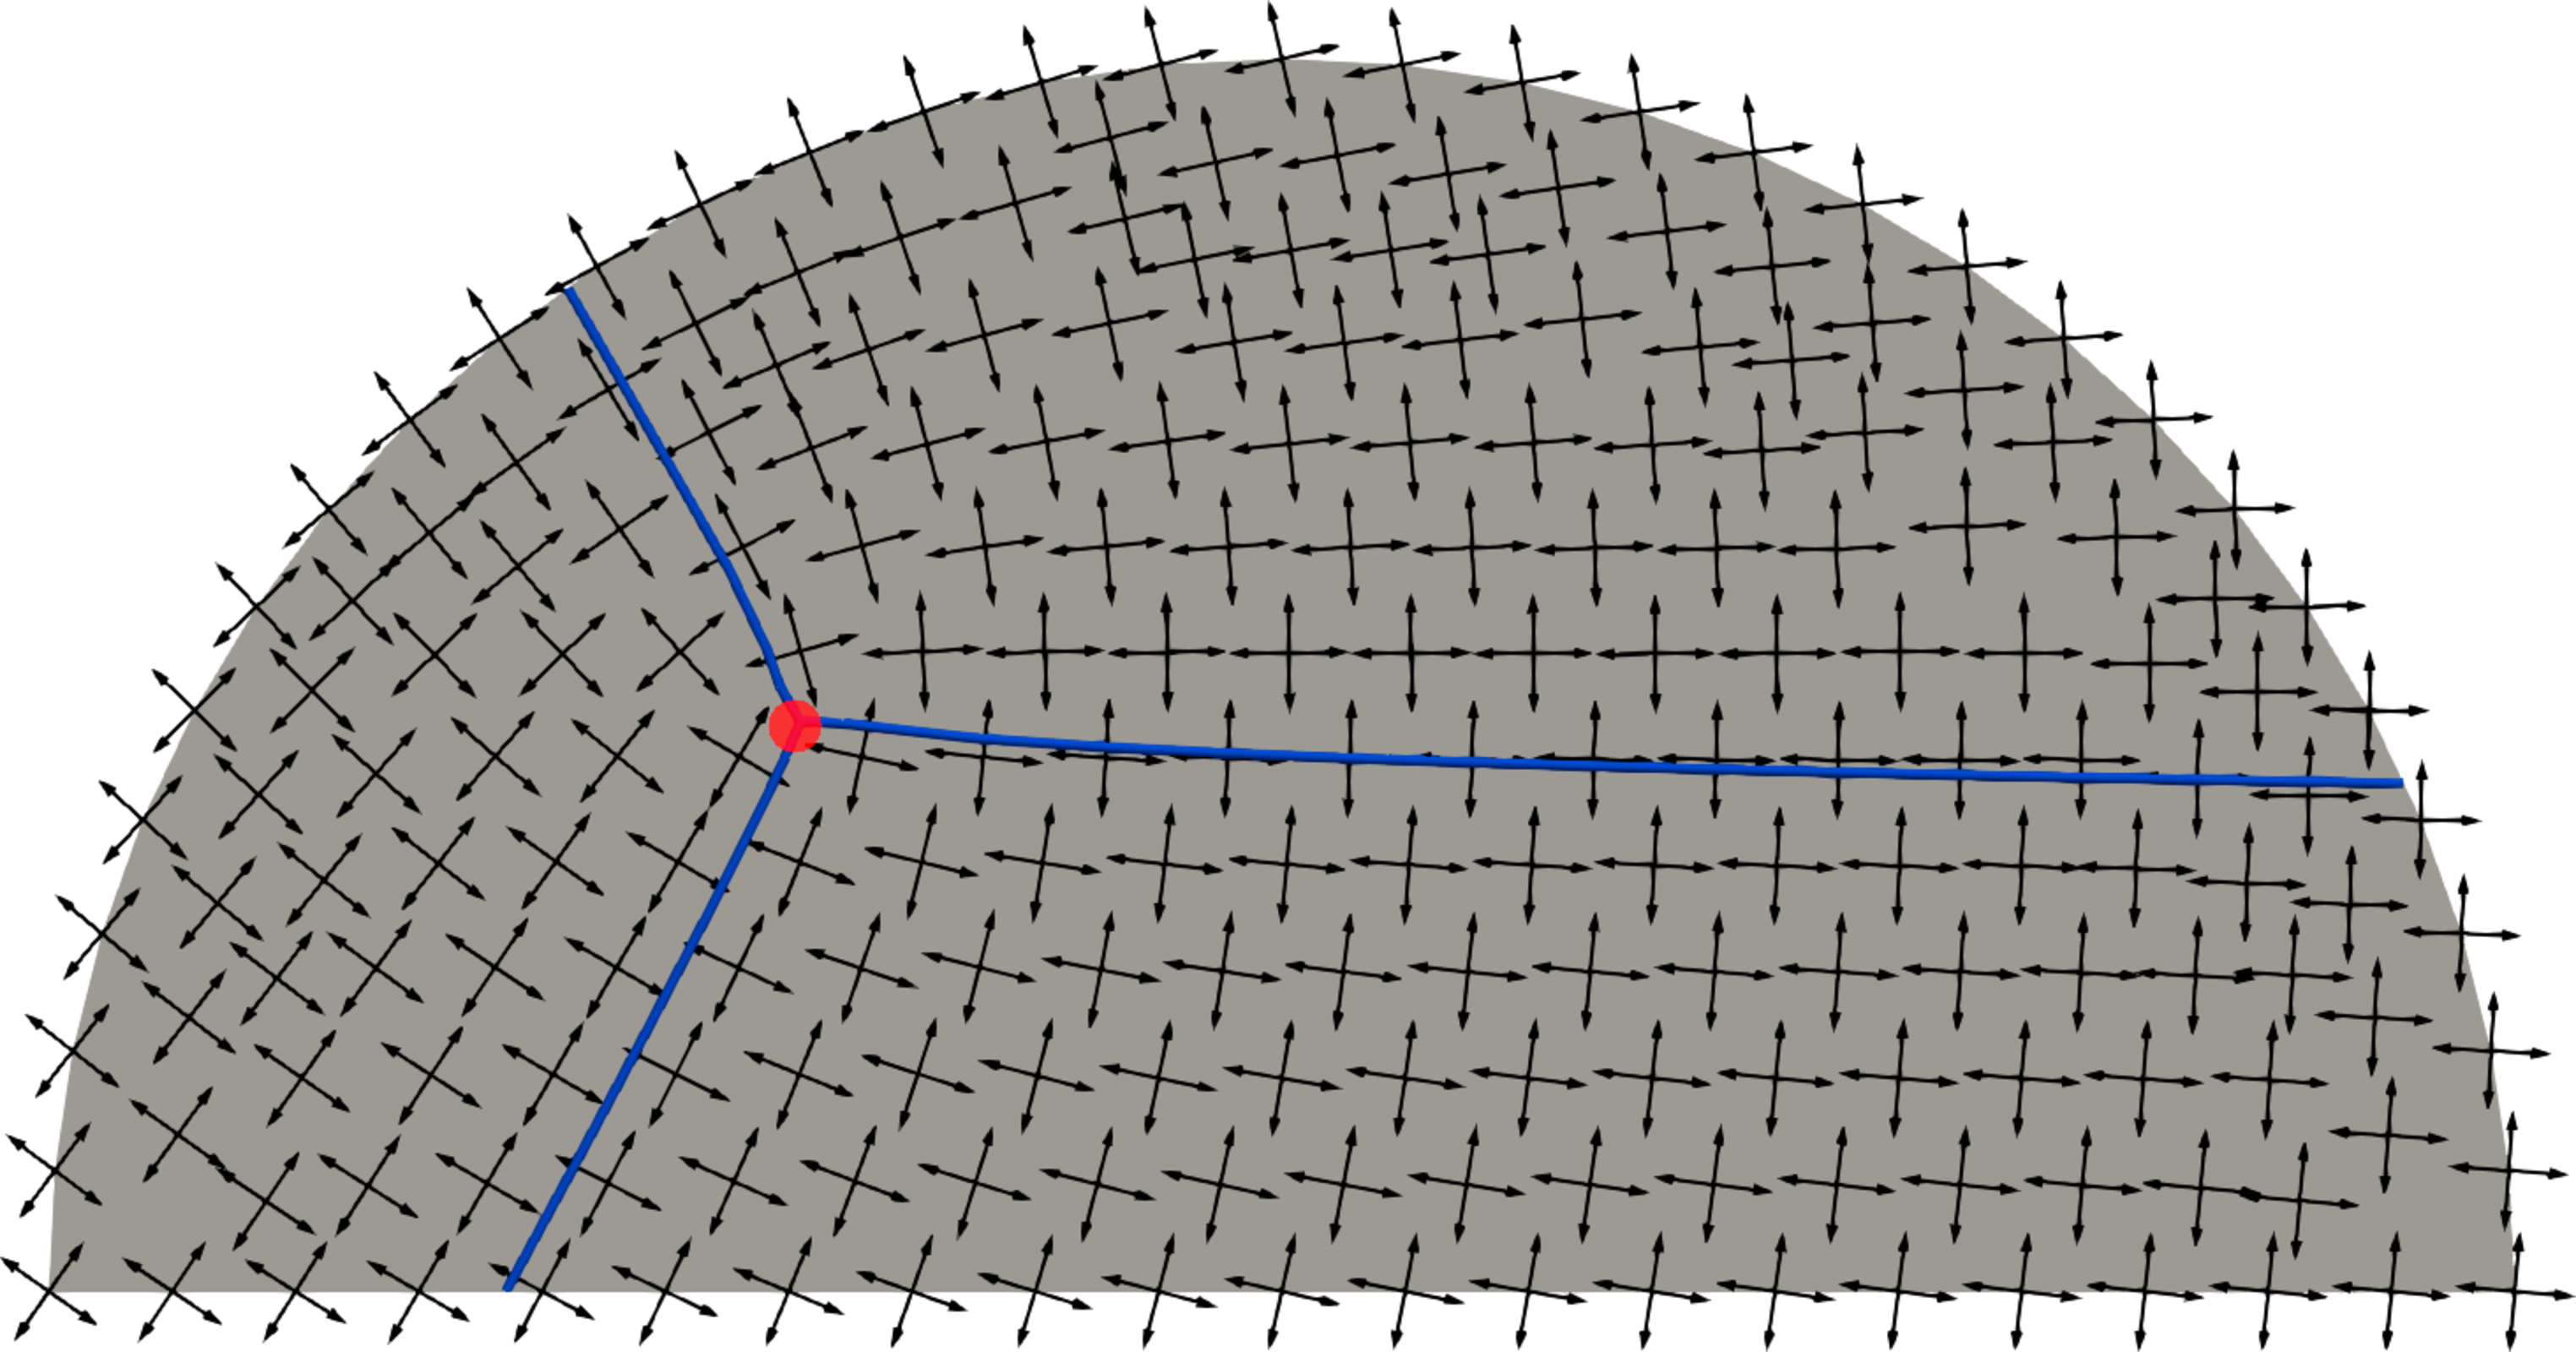
\includegraphics[width=\textwidth]{images/demi_disc_first_phi_first.pdf}
    \caption{Champ de croix initial avec un point singulier interne d'indice $1/4$.}
    \label{fig:demi_disc_first_cond_phi_first}
\end{subfigure}
\\[0.4cm]
\begin{subfigure}{0.65\textwidth}
    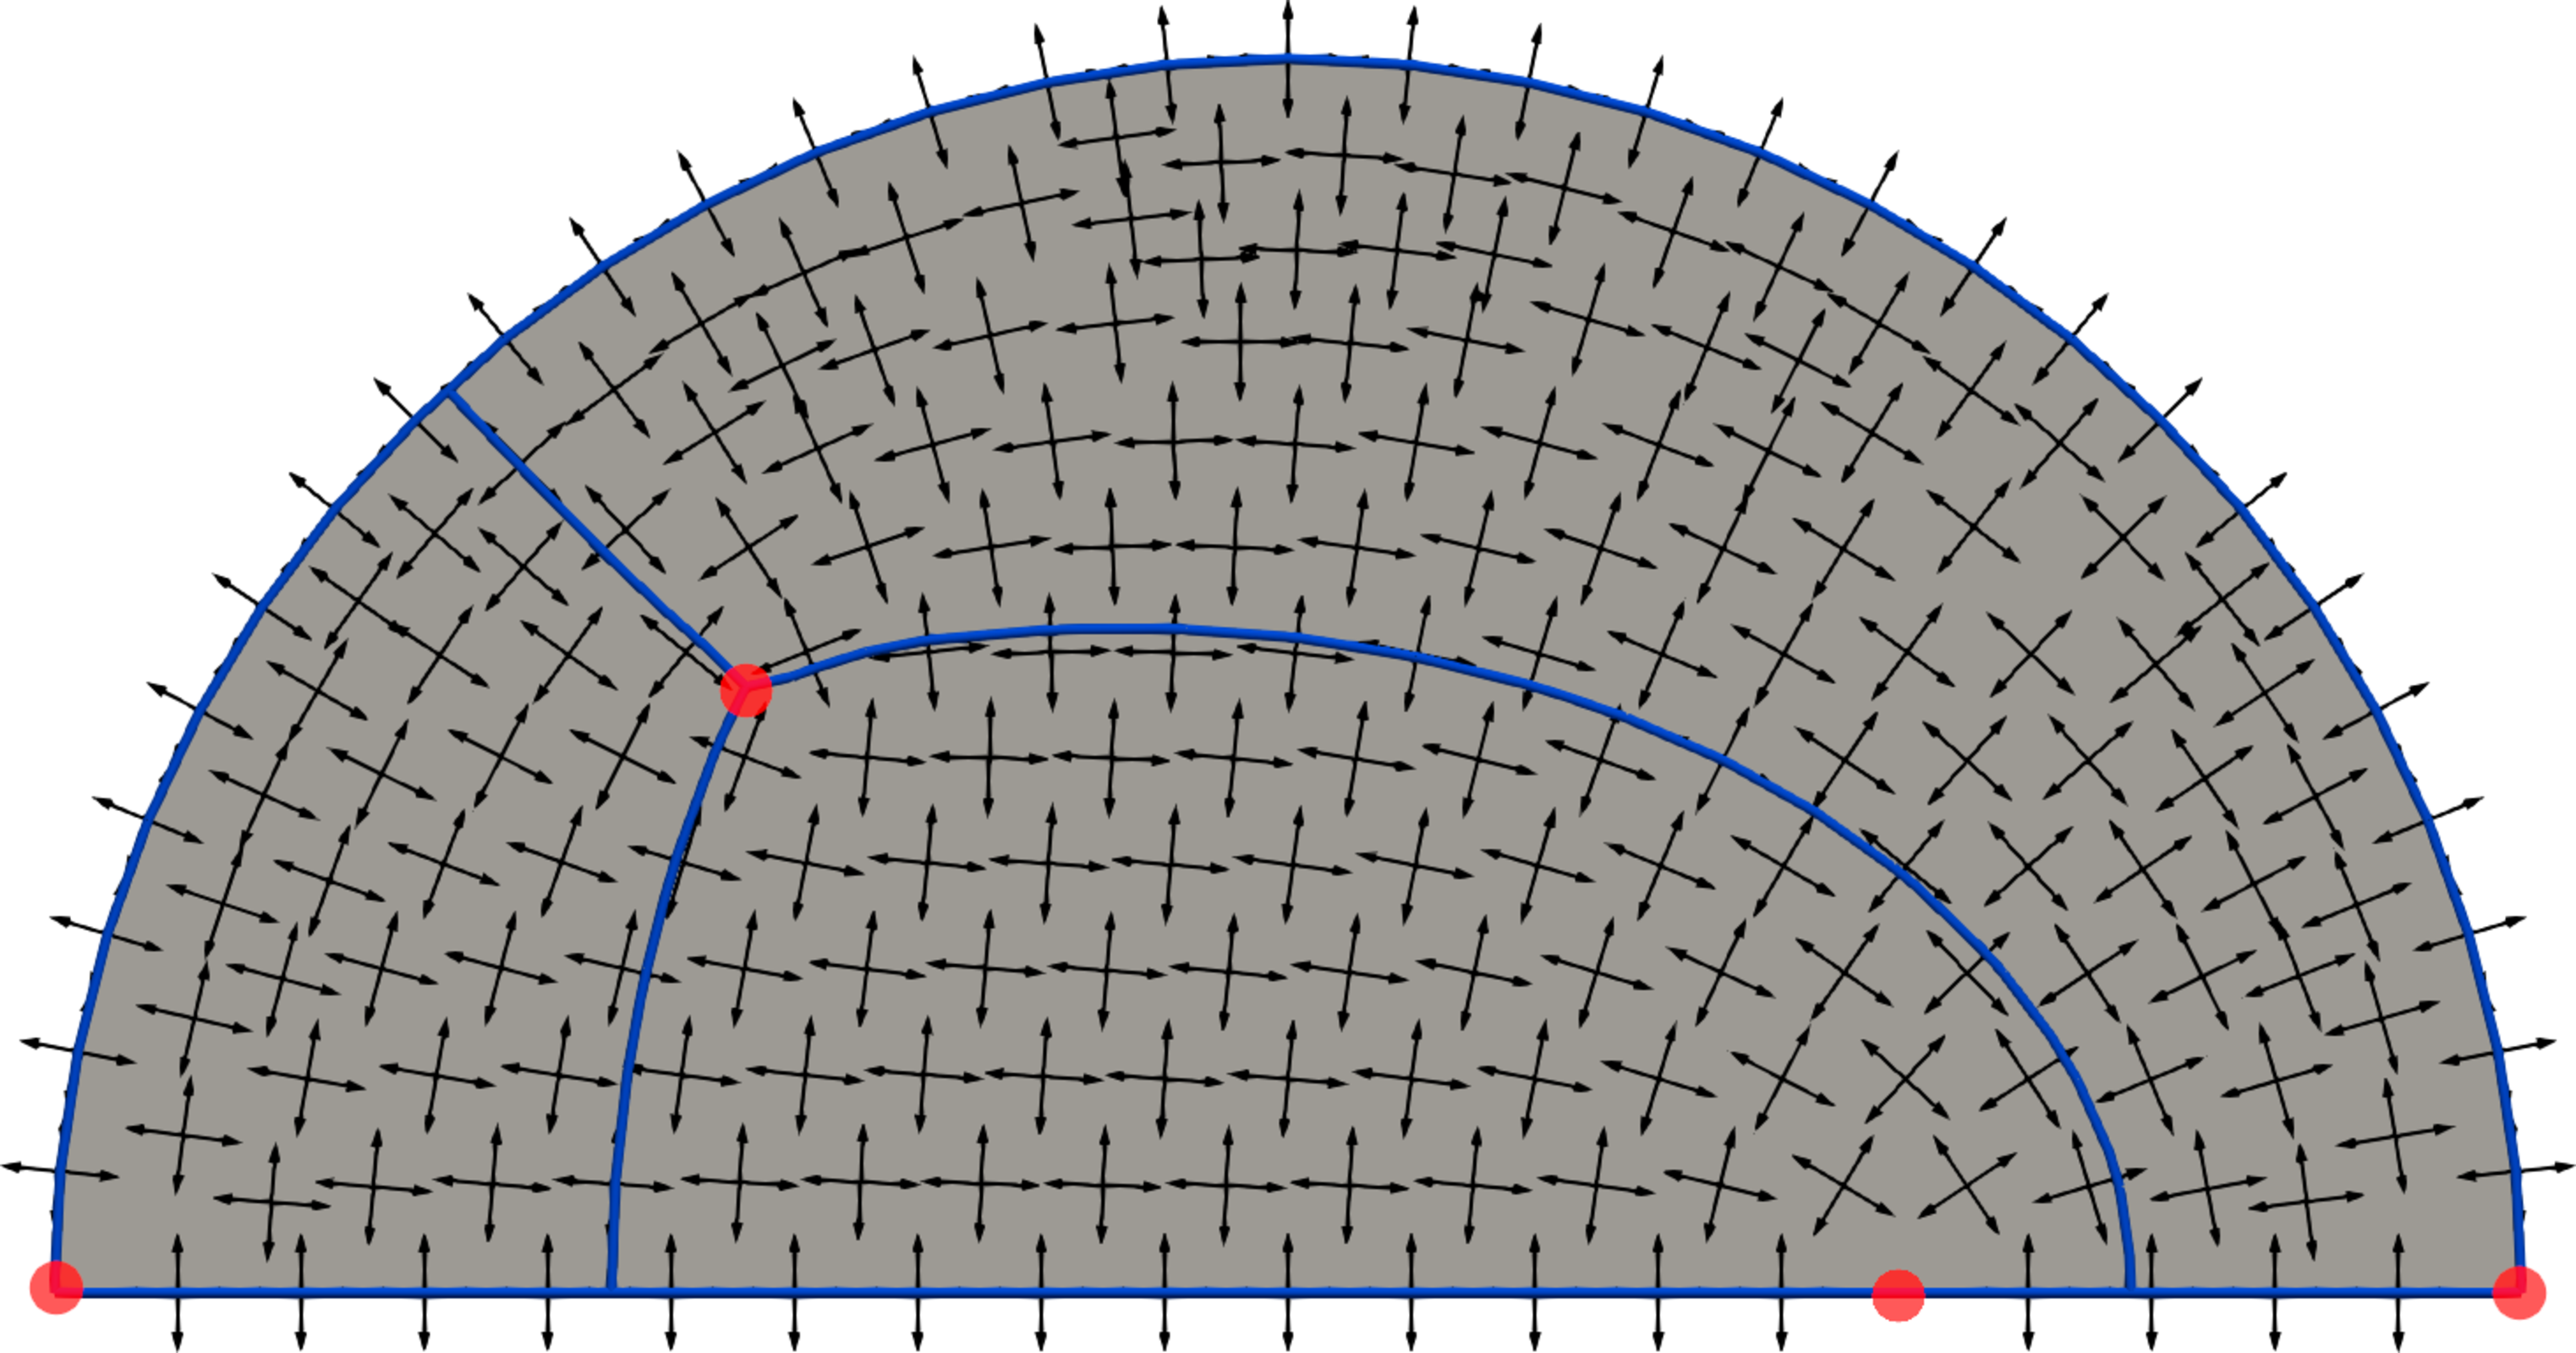
\includegraphics[width=\textwidth]{images/demi_disc_first_phi_second.pdf}
    \caption{Alignement du champ de croix initial sur le bord du domaine et partitionnement du domaine.}
    \label{fig:demi_disc_first_cond_phi_second}
\end{subfigure}
\\[0.4cm]
\begin{subfigure}{0.65\textwidth}
    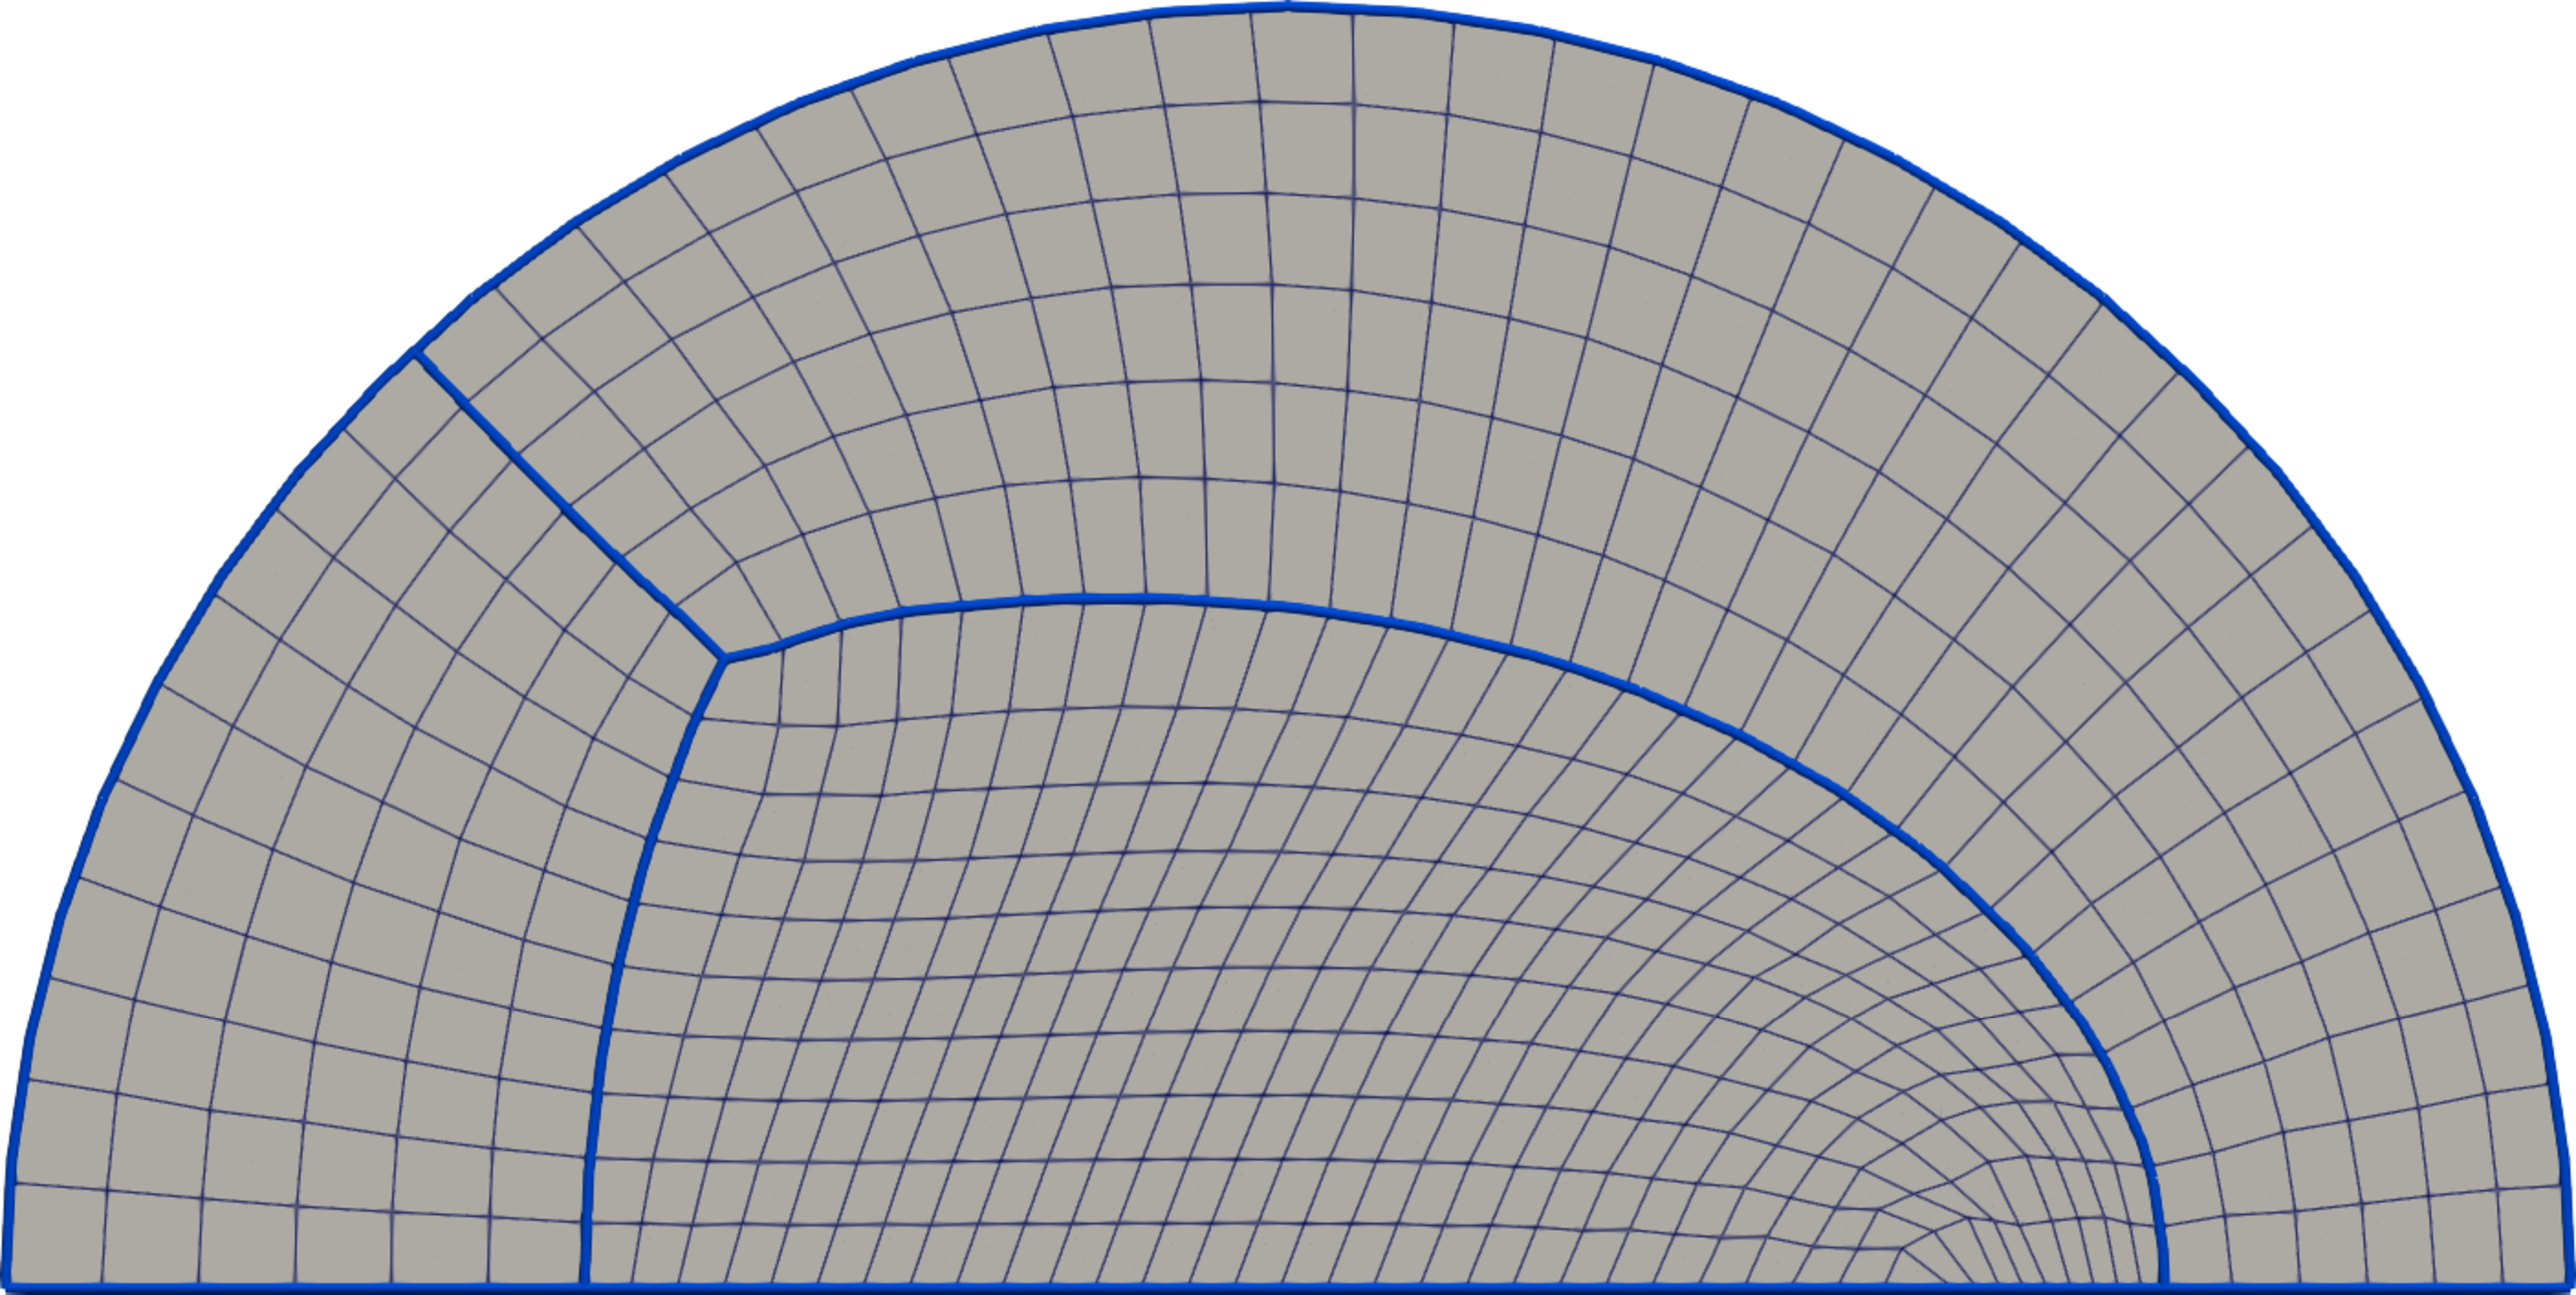
\includegraphics[width=\textwidth]{images/demi_disc_first_phi_third.pdf}
    \caption{Maillage quadilatéral du domaine présentant un quadrangle dégénéré.}
    \label{fig:demi_disc_first_cond_phi_third}
\end{subfigure}

\caption{Illustration de l'opération d'alignement à partir du champ d'angle donné par l'équation \eqref{eqn:first_phi_computation}.}
\label{fig:demi_disc_first_cond_phi}
\end{figure}

En l'état, nous n'avons donc aucun contrôle sur la régularité de cette condition de bord, ce qui entraînera des effets indésirables dans le maillage quadrilatéral construit à partir du partitionnement obtenu. Par exemple, sur la figure \ref{fig:demi_disc_first_cond_phi}, nous considérons un champ de croix initial possédant une singularité d'indice $1/4$ à l'intérieur du domaine (figure \ref{fig:demi_disc_first_cond_phi_first}). Le champ d'alignement est calculé avec l'équation \eqref{eqn:first_phi_computation}, puis le champ de croix $\bar{v}$ est construit. On observe clairement que $\bar{v}$ est bien aligné avec le bord du domaine et conserve la singularité interne du champ de croix initial. Cependant, on remarque l'apparition de singularités de bord dans le champ de croix $\bar{v}$. En appliquant l'algorithme de partitionnement \ref{alg:algo_main} sur $\bar{v}$, le partitionnement obtenu présente des régions à quatre côtés (figure \ref{fig:demi_disc_first_cond_phi_second}) mais, la présence de points singuliers de bord non contrôlés (en termes de positionnement et d'indice) conduit à un maillage quadrilatéral comportant des quadrangles dégénérés (figure \ref{fig:demi_disc_first_cond_phi_third}).


Afin de contrôler cette situation, nous allons modifier le processus d'alignement en ajustant la condition de Dirichlet de l'équation \eqref{eqn:first_phi_computation} et en imposant des conditions sur le champ de croix initial $\bar{u}$.

Pour commencer, nous associons à chaque point $p\in\partial\Omega$, un paramètre $I_p$ vérifiant:
\begin{equation}
I_p=\displaystyle\frac{k}{4}\mbox{ avec }k\in\mathbb{Z}\mbox{ et }k\leq 1
\end{equation}
Ce paramètre représente l'indice désiré pour les points de bord dans le champ de croix $\bar{v}$ (une fois l'opération d'alignement réalisée). Un critère a priori pour le choix automatique de ce paramètre sera exposé ultérieurement dans la sous-section \ref{subsec:sing_bord}. Nous définissons ensuite l'ensemble $\mathcal{B}$ qui regroupe les points pour lesquels le paramètre $I_p\neq 0$. Ces points seront singuliers dans le champ de croix $\bar{v}$ (une fois l'opération d'alignement réalisée). %L'ensemble $\mathcal{B}$ doit aussi inclure les points singuliers du champ $\bar{n}$. Ces points étant déjà singulier dans $\bar{n}$, ils resteront singuliers dans $\bar{v}$ après l'opération d'alignement.
Pour finir, il est impératif que le champ de croix $\bar{u}$ ainsi que l'ensemble $\mathcal{B}$ satisfassent:\\
\begin{itemize}
 \item[$\bullet$] $0< Card(\mathcal{S}_{\bar{u}})+Card(\mathcal{B})< \infty$,\\
 \item[$\bullet$] Pour tout point $p\in\mathcal{S}_{\bar{u}}$, $id_{\bar{u}}(p)=k/4$, avec $k\in\mathbb{Z}$ et $k\leq 1$,\\
 \item[$\bullet$] Soit $\gamma$ une paramétrisation de $\partial\Omega$ dans le sens positif. Il existe $\theta_{\bar{u}}^\gamma$ vérifiant:
 \begin{equation}
    \label{eqn:principe_hypothese_u}
    \theta_{\bar{u}}^\gamma(1)-\theta_{\bar{u}}^\gamma(0)=2\pi\chi(\Omega)-2\pi\sum_{p\in\mathcal{B}}I_p.
\end{equation}
\end{itemize}
L'opération d'alignement est alors formulé de la manière suivante:\\\\
\textbf{Opération d'alignement:} étant donné $\bar{u}$, nous définissons le champ de croix $\bar{v}$ pour tout $p\in\Omega$ par:
\begin{equation}
\bar{v}(p)=
\left\{
\begin{array}{ll}
\mathbf{R}(\phi(p))\bar{u}(p) & \mbox{ si } p\in\Omega\backslash(\mathcal{B}\cup\mathcal{S}_{\bar{n}}\cup\mathcal{S}_{\bar{u}}),\\[0.5cm]
\bar{n}(p) & \mbox{ si } p\in(\mathcal{S}_{\bar{u}}\cap\partial\Omega)\backslash(\mathcal{B}\cup\mathcal{S}_{\bar{n}}),\\[0.5cm]
0 & \mbox{ si } p\in\mathcal{B}\cup\mathcal{S}_{\bar{n}}.
\end{array}
\right.
\label{eqn:principe_def_v}
\end{equation}
où $\phi:\Omega\longrightarrow\mathbb{R}$ est définie comme la solution de l'équation de Laplace suivante:
\begin{equation}
\left\{
\begin{array}{lcll}
\Delta\phi &=& 0 &\mbox{ dans }\Omega,\\[0.5cm]
\phi(\gamma(t))&=&\theta_{\bar{n}}^\gamma(t)+\mathcal{I}(t)-\theta_{\bar{u}}^\gamma(t)& \mbox{ sur } \gamma^{-1}(\partial\Omega\backslash(\mathcal{B}\cup\mathcal{S}_{\bar{n}}\cup\mathcal{S}_{\bar{u}})),
\end{array}
\right.
\label{eqn:principe_def_phi}
\end{equation}
où la fonction $\mathcal{I}$ est donnée pour tout $t\in\gamma^{-1}(\partial\Omega\backslash(\mathcal{B}\cup\mathcal{S}_{\bar{n}}\cup\mathcal{S}_{\bar{u}}))$ par:
$$
\mathcal{I}(t)=\sum_{s\in\gamma^{-1}(\mathcal{B}\cup\mathcal{S}_{\bar{n}})}\left[\left(\pi-\widehat{\gamma(s)}-2\pi I_{\gamma(s)}\right)-\left(\lim\limits_{r\rightarrow s^+}\theta^{\gamma}_{\bar{n}}(r) - \lim\limits_{r\rightarrow s^-}\theta^{\gamma}_{\bar{n}}(r)\right)\right]\mathbb{1}_{[0, t]}(s),
$$
avec $\widehat{\gamma(s)}$ la mesure de l'ouverture angulaire de la frontière en $\gamma(s)$.

\begin{figure}[!h]
\centering
\begin{subfigure}{0.65\textwidth}
    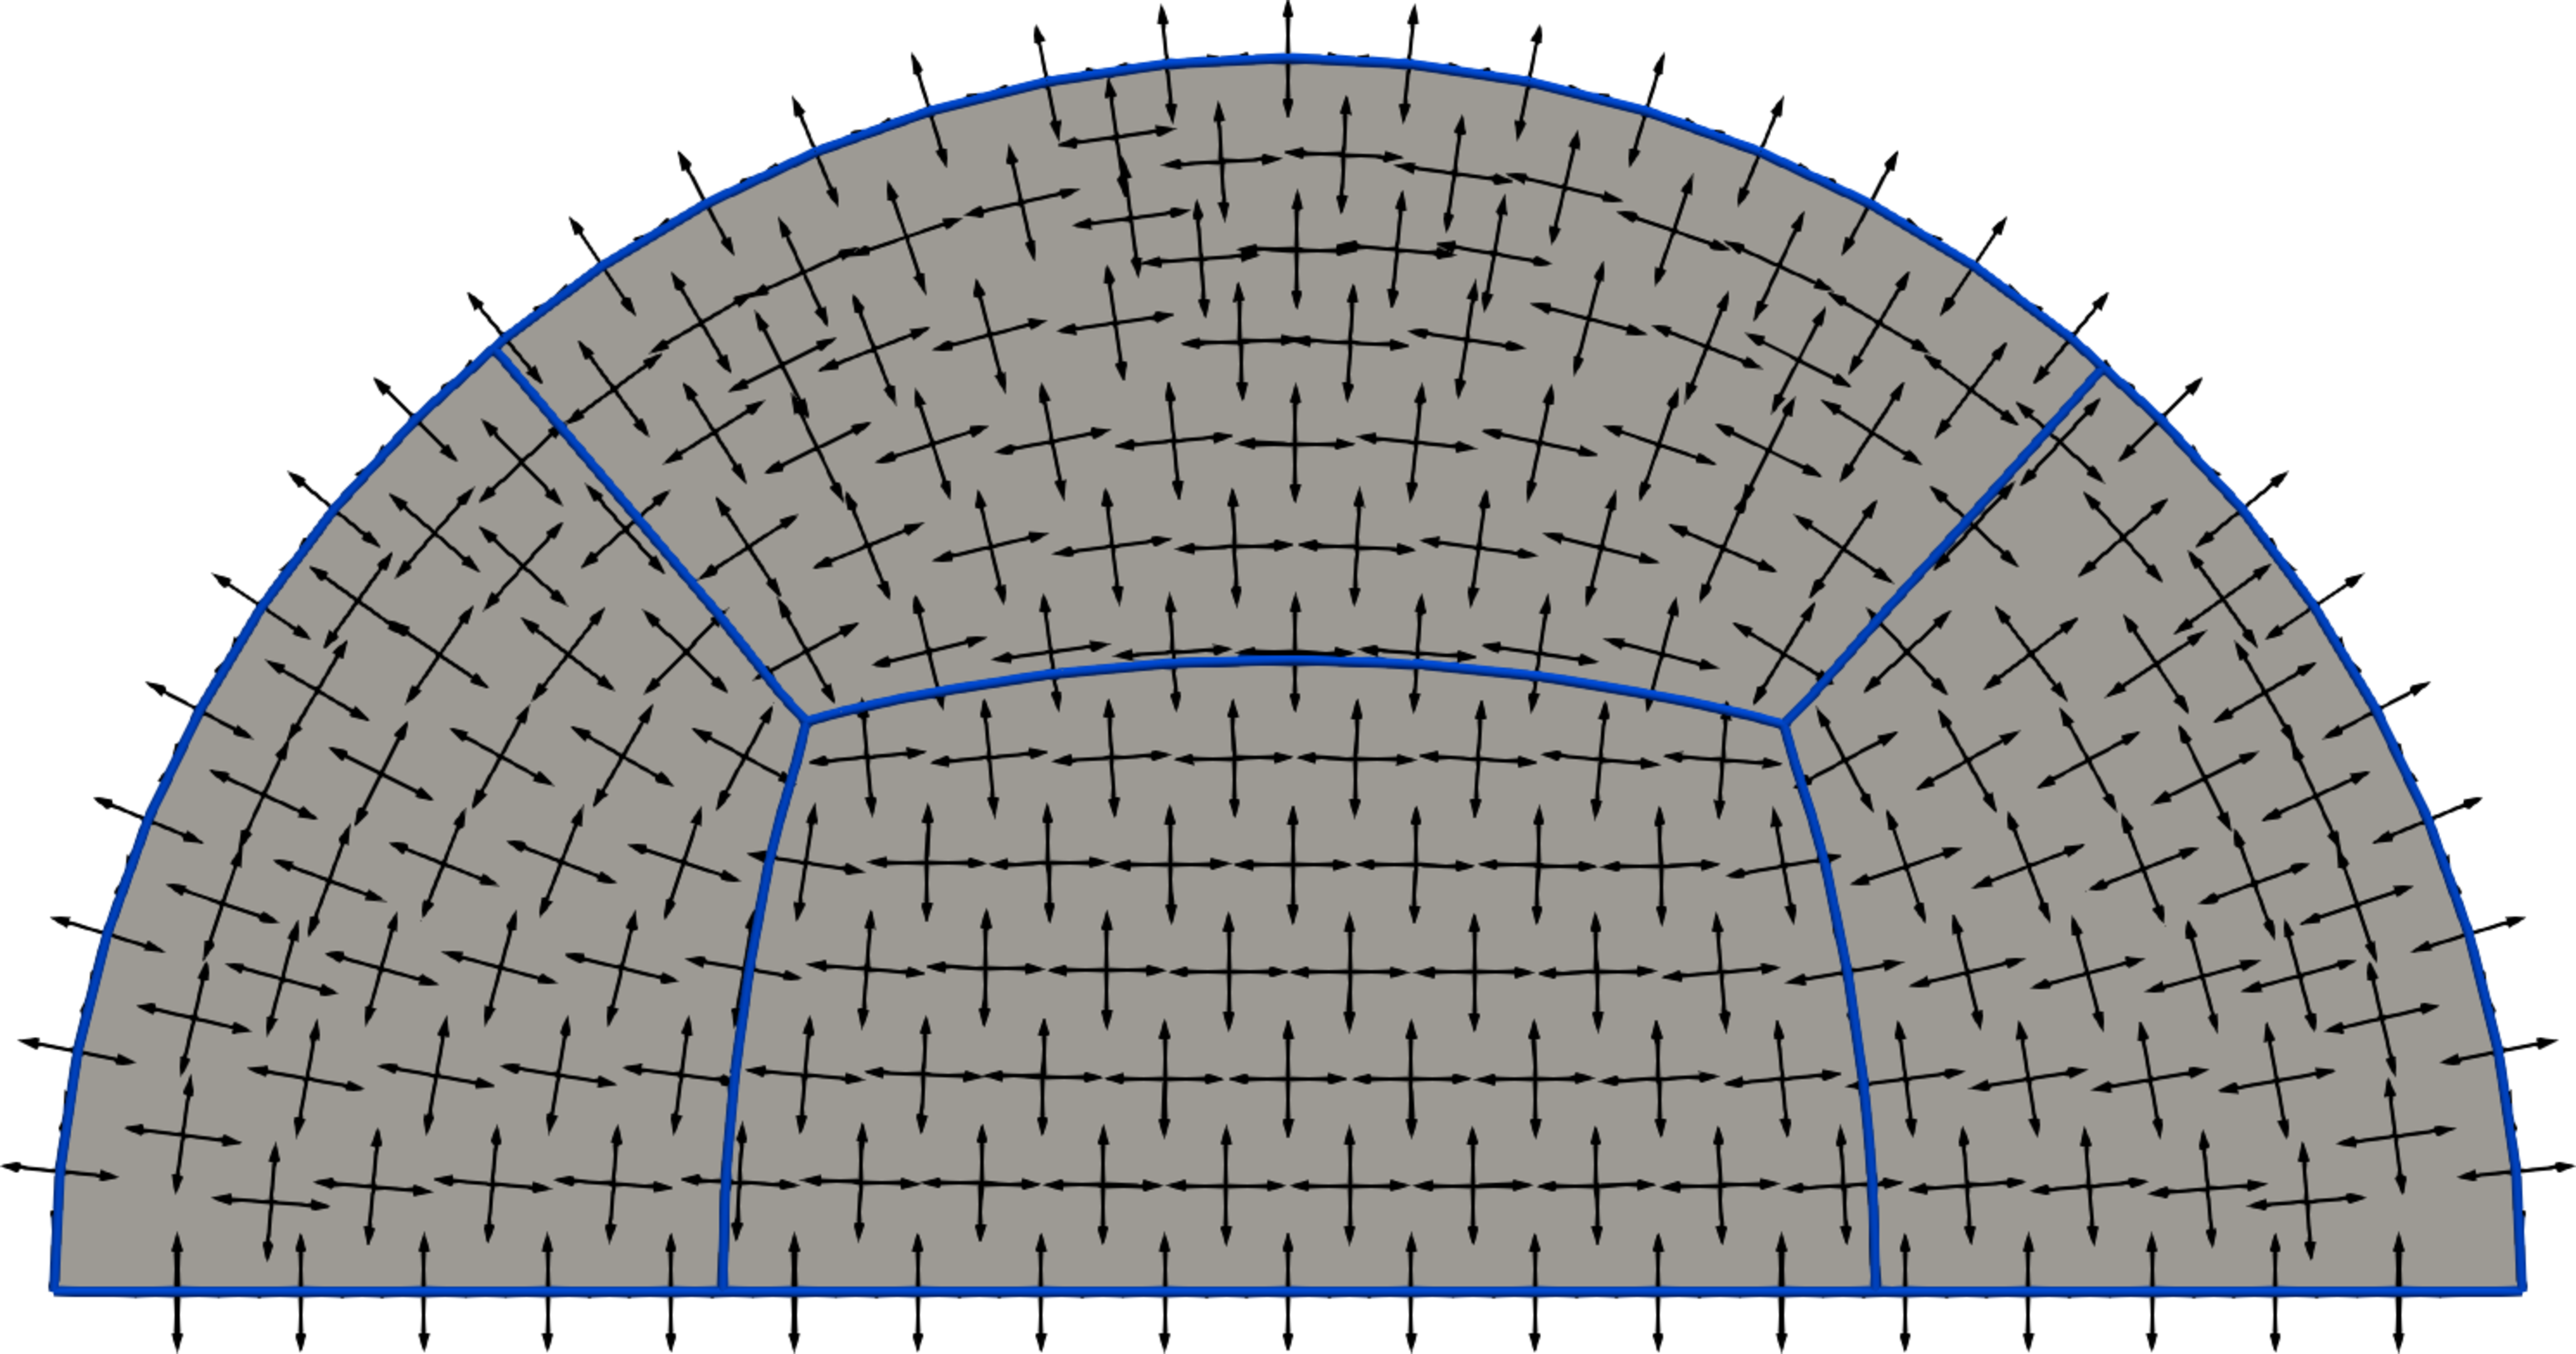
\includegraphics[width=\textwidth]{images/demi_disc_second_phi_first.pdf}
    \caption{Alignement du champ de croix présenté sur la figure \ref{fig:demiDisc_valProp_mauvaix_decoup} sur le bord du domaine et partitionnement du domaine.}
    \label{fig:demi_disc_second_cond_phi_first}
\end{subfigure}
\\[0.3ex]
\begin{subfigure}{0.65\textwidth}
    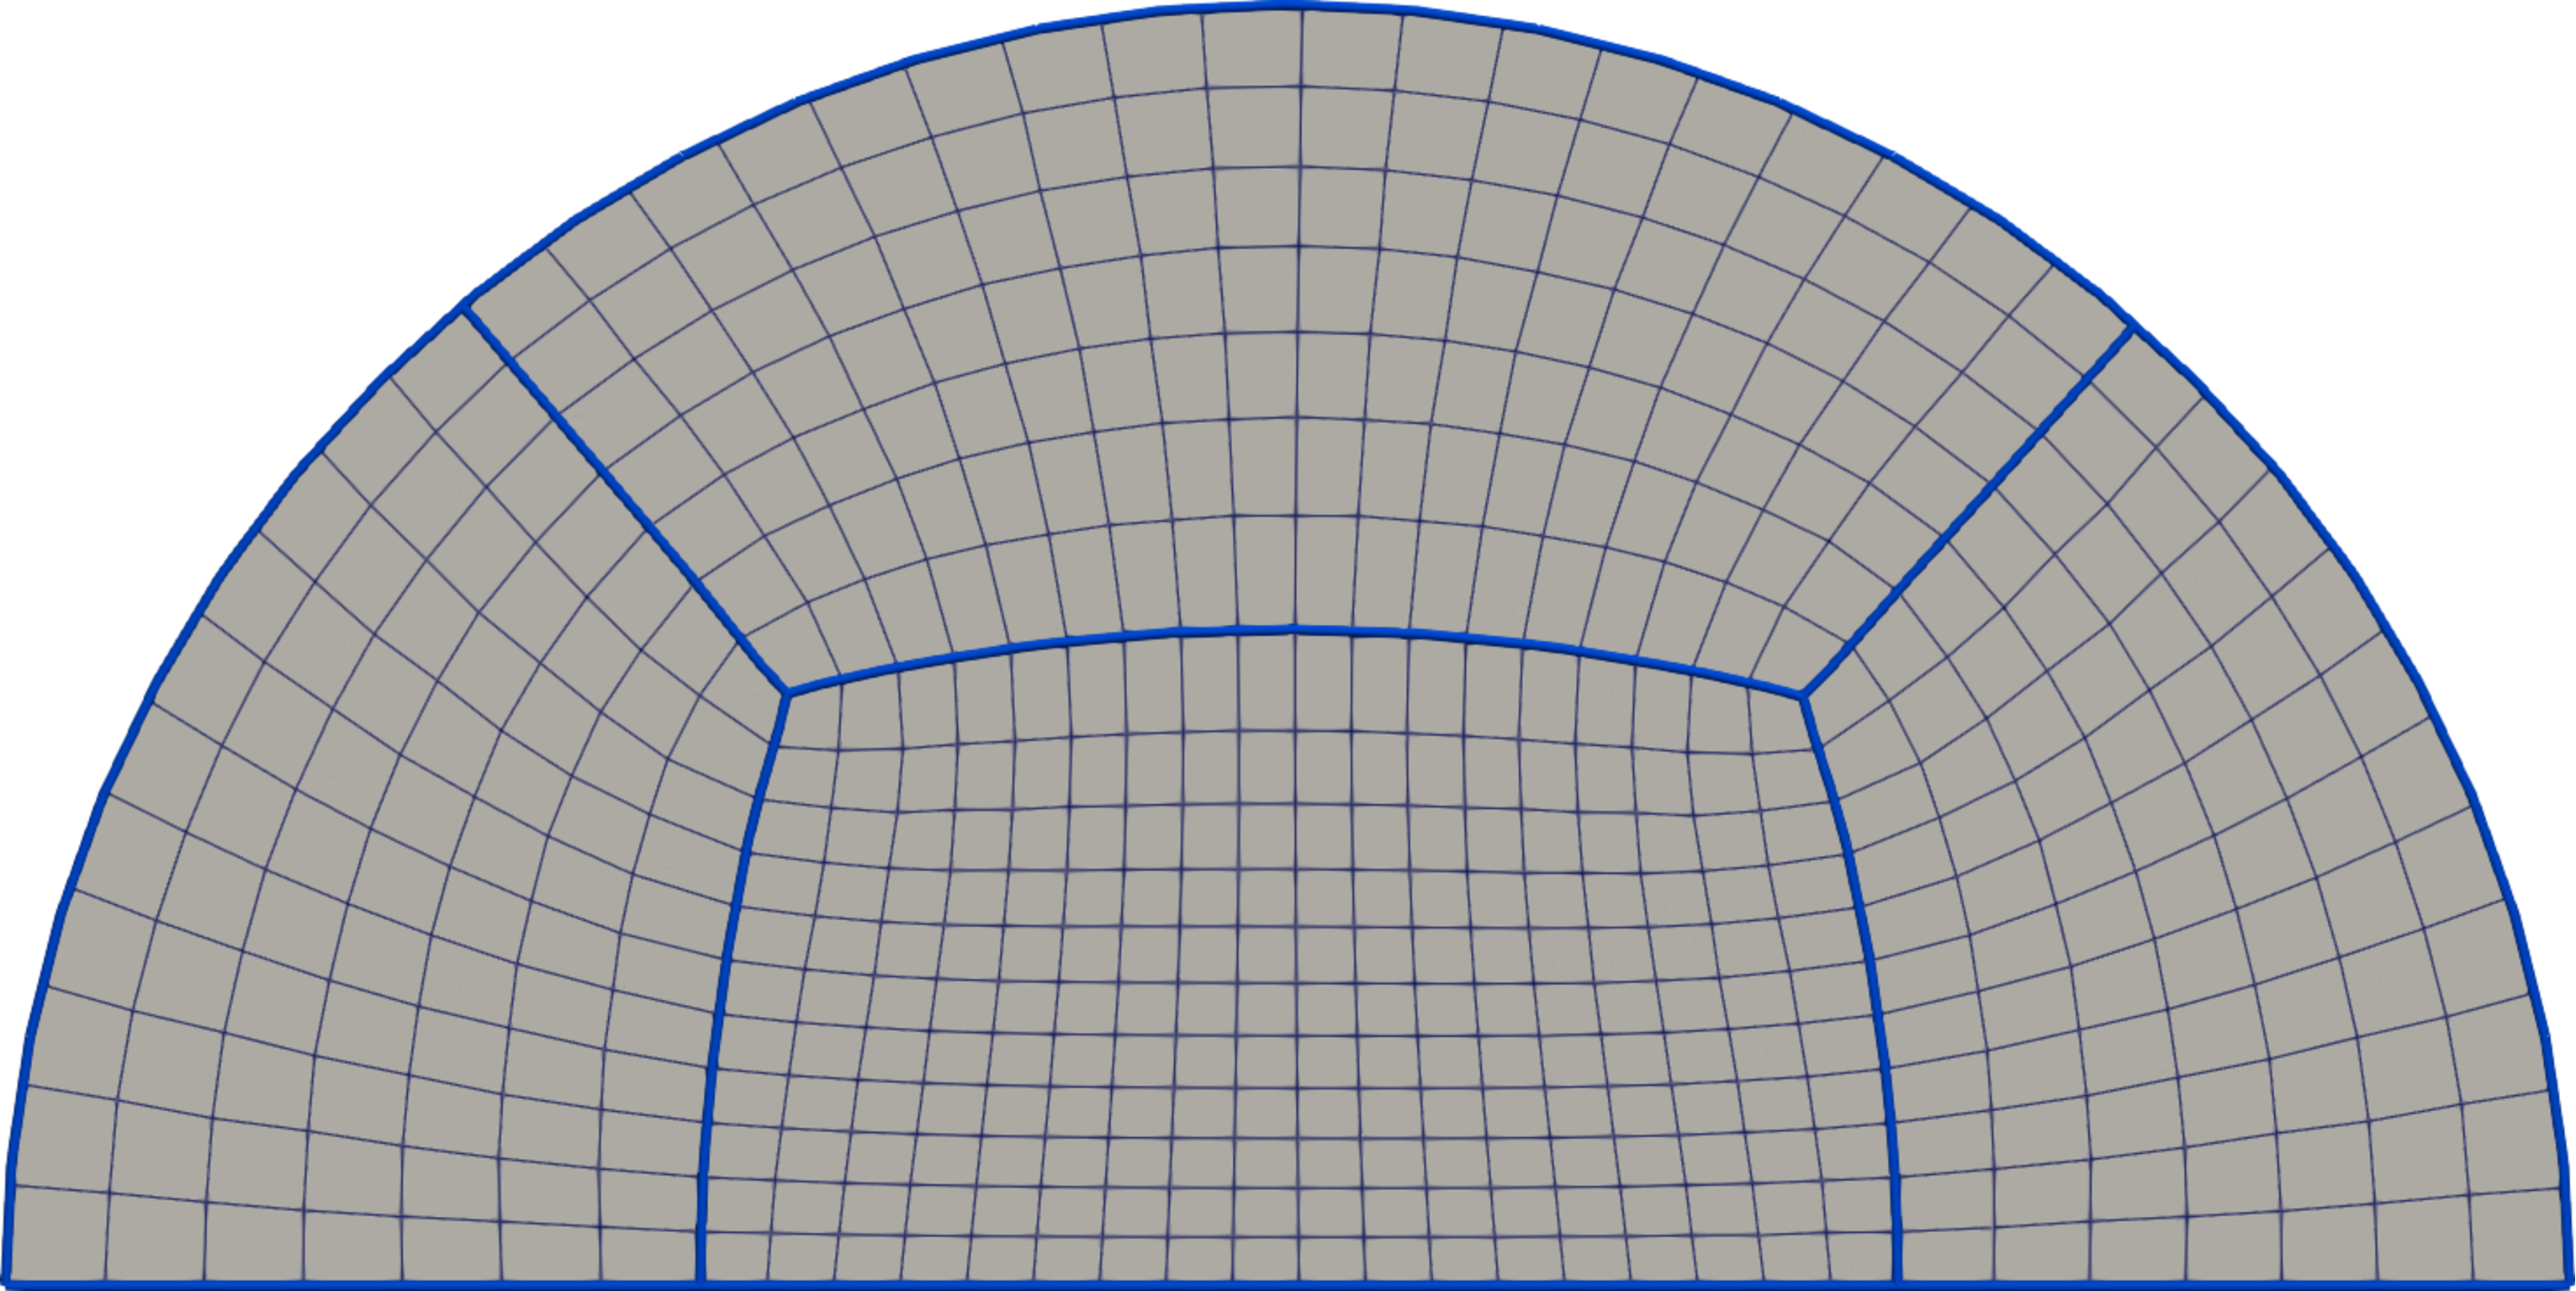
\includegraphics[width=\textwidth]{images/demi_disc_second_phi_second.pdf}
    \caption{Maillage quadrilatéral du domaine.}
    \label{fig:demi_disc_second_cond_phi_second}
\end{subfigure}
\caption{Illustration de l'opération d'alignement à partir du champ d'angle donné par l'équation \eqref{eqn:principe_def_phi}.}
\label{fig:demi_disc_second_cond_phi}
\end{figure}

\begin{remark}
    \[\]
    \vspace{-1cm}
    \begin{enumerate}
        \item On montre (voir le Théorème \ref{thm:theorem2}) que le champ de croix $\bar{v}$ est aligné par rapport à $\partial\Omega$. On se ramène ainsi au cas du champ de croix aligné sur le bord de $\Omega$ et l'application l'algorithme \ref{alg:algo_main} permet d'obtenir un partitionnement de $\Omega$ en régions de quatre côtés lorsque les séparatrices ne convergent pas en cycles limites.\\
        \item Le champ de croix $\bar{v}$ conserve certaines caractéristiques du champ de croix $\bar{u}$. Ainsi $\bar{v}$ est un champ de croix presque-$\mathcal{C}^1$ sur $\Omega$. De plus pour tout $p\in\Omega$, $id_{\bar{v}}(p)=id_{\bar{u}}(p)$ et pour tout $p\in\partial\Omega$, $id^\partial_{\bar{v}}(p)=I_p$.\\
        \item La condition \eqref{eqn:principe_hypothese_u} permet de garantir que $\phi(\gamma(1))-\phi(\gamma(0))=0$ (voir le lemme \ref{lem:marvelous_lemma}) nécessaire pour garantir que le point $p=\gamma(0)=\gamma(1)$ satisfait $id_{\bar{v}}(p)=I_p$.%integrale dphi egale 0 car hypothese sur u garantissant ainsi idv=I Controle on trouve ce qui est prescrit on peut donc evider des quadrangle degenerer en choisissant le bon I en fonction la courbure locale en chaque point
    \end{enumerate}
\end{remark}

 L'algorithme suivant résume le procédé.

\vspace{0.5cm}
\begin{algorithm}[H]
\label{alg:algo_simply_connected}
\SetKwInOut{Input}{Entrée}
\SetKwInOut{Output}{Sortie}
\Input{$\Omega$ un domaine borné et fermé simplement connexe, champ de croix $\bar{u}$ défini sur $\Omega$, ensemble $\mathcal{B}$, paramètre $I_p$ pour tout $p\in\partial\Omega$.}
\Output{Partition de $\Omega$ en ensembles de régions.}
\vspace{0.2cm}
1.) Calcul du champ d'alignement (voir l'équation \eqref{eqn:principe_def_phi}),\\\vspace{0.2cm}
2.) Calcul du champ de croix $\bar{v}$ (voir l'équation \eqref{eqn:principe_def_v}),\\\vspace{0.2cm}
3.) Application de l'algorithme \ref{alg:algo_main} au champ de croix $\bar{v}$.\\\vspace{0.2cm}
\caption{Algorithme de partitionnement pour un domaine simplement connexe basé sur un champ de croix non aligné}
\end{algorithm}
\vspace{0.5cm}

En appliquant cet algorithme au champ de croix représenté sur la figure \ref{fig:demiDisc_valProp_mauvaix_decoup}, nous obtenons le partitionnement illustré sur la figure \ref{fig:demi_disc_second_cond_phi}. Un autre exemple est présenté sur la figure \ref{fig:rect_demi_disc}. Dans ce cas, le champ de croix initial possède deux points singuliers d'indice $-1/4$. L'ensemble $\mathcal{B}$ correspond aux coins du domaine, auxquels nous avons associé le paramètre $I_p=1/4$ pour tout $p\in\mathcal{B}$.



\begin{figure}[!h]
\centering
\begin{subfigure}{0.58\textwidth}
    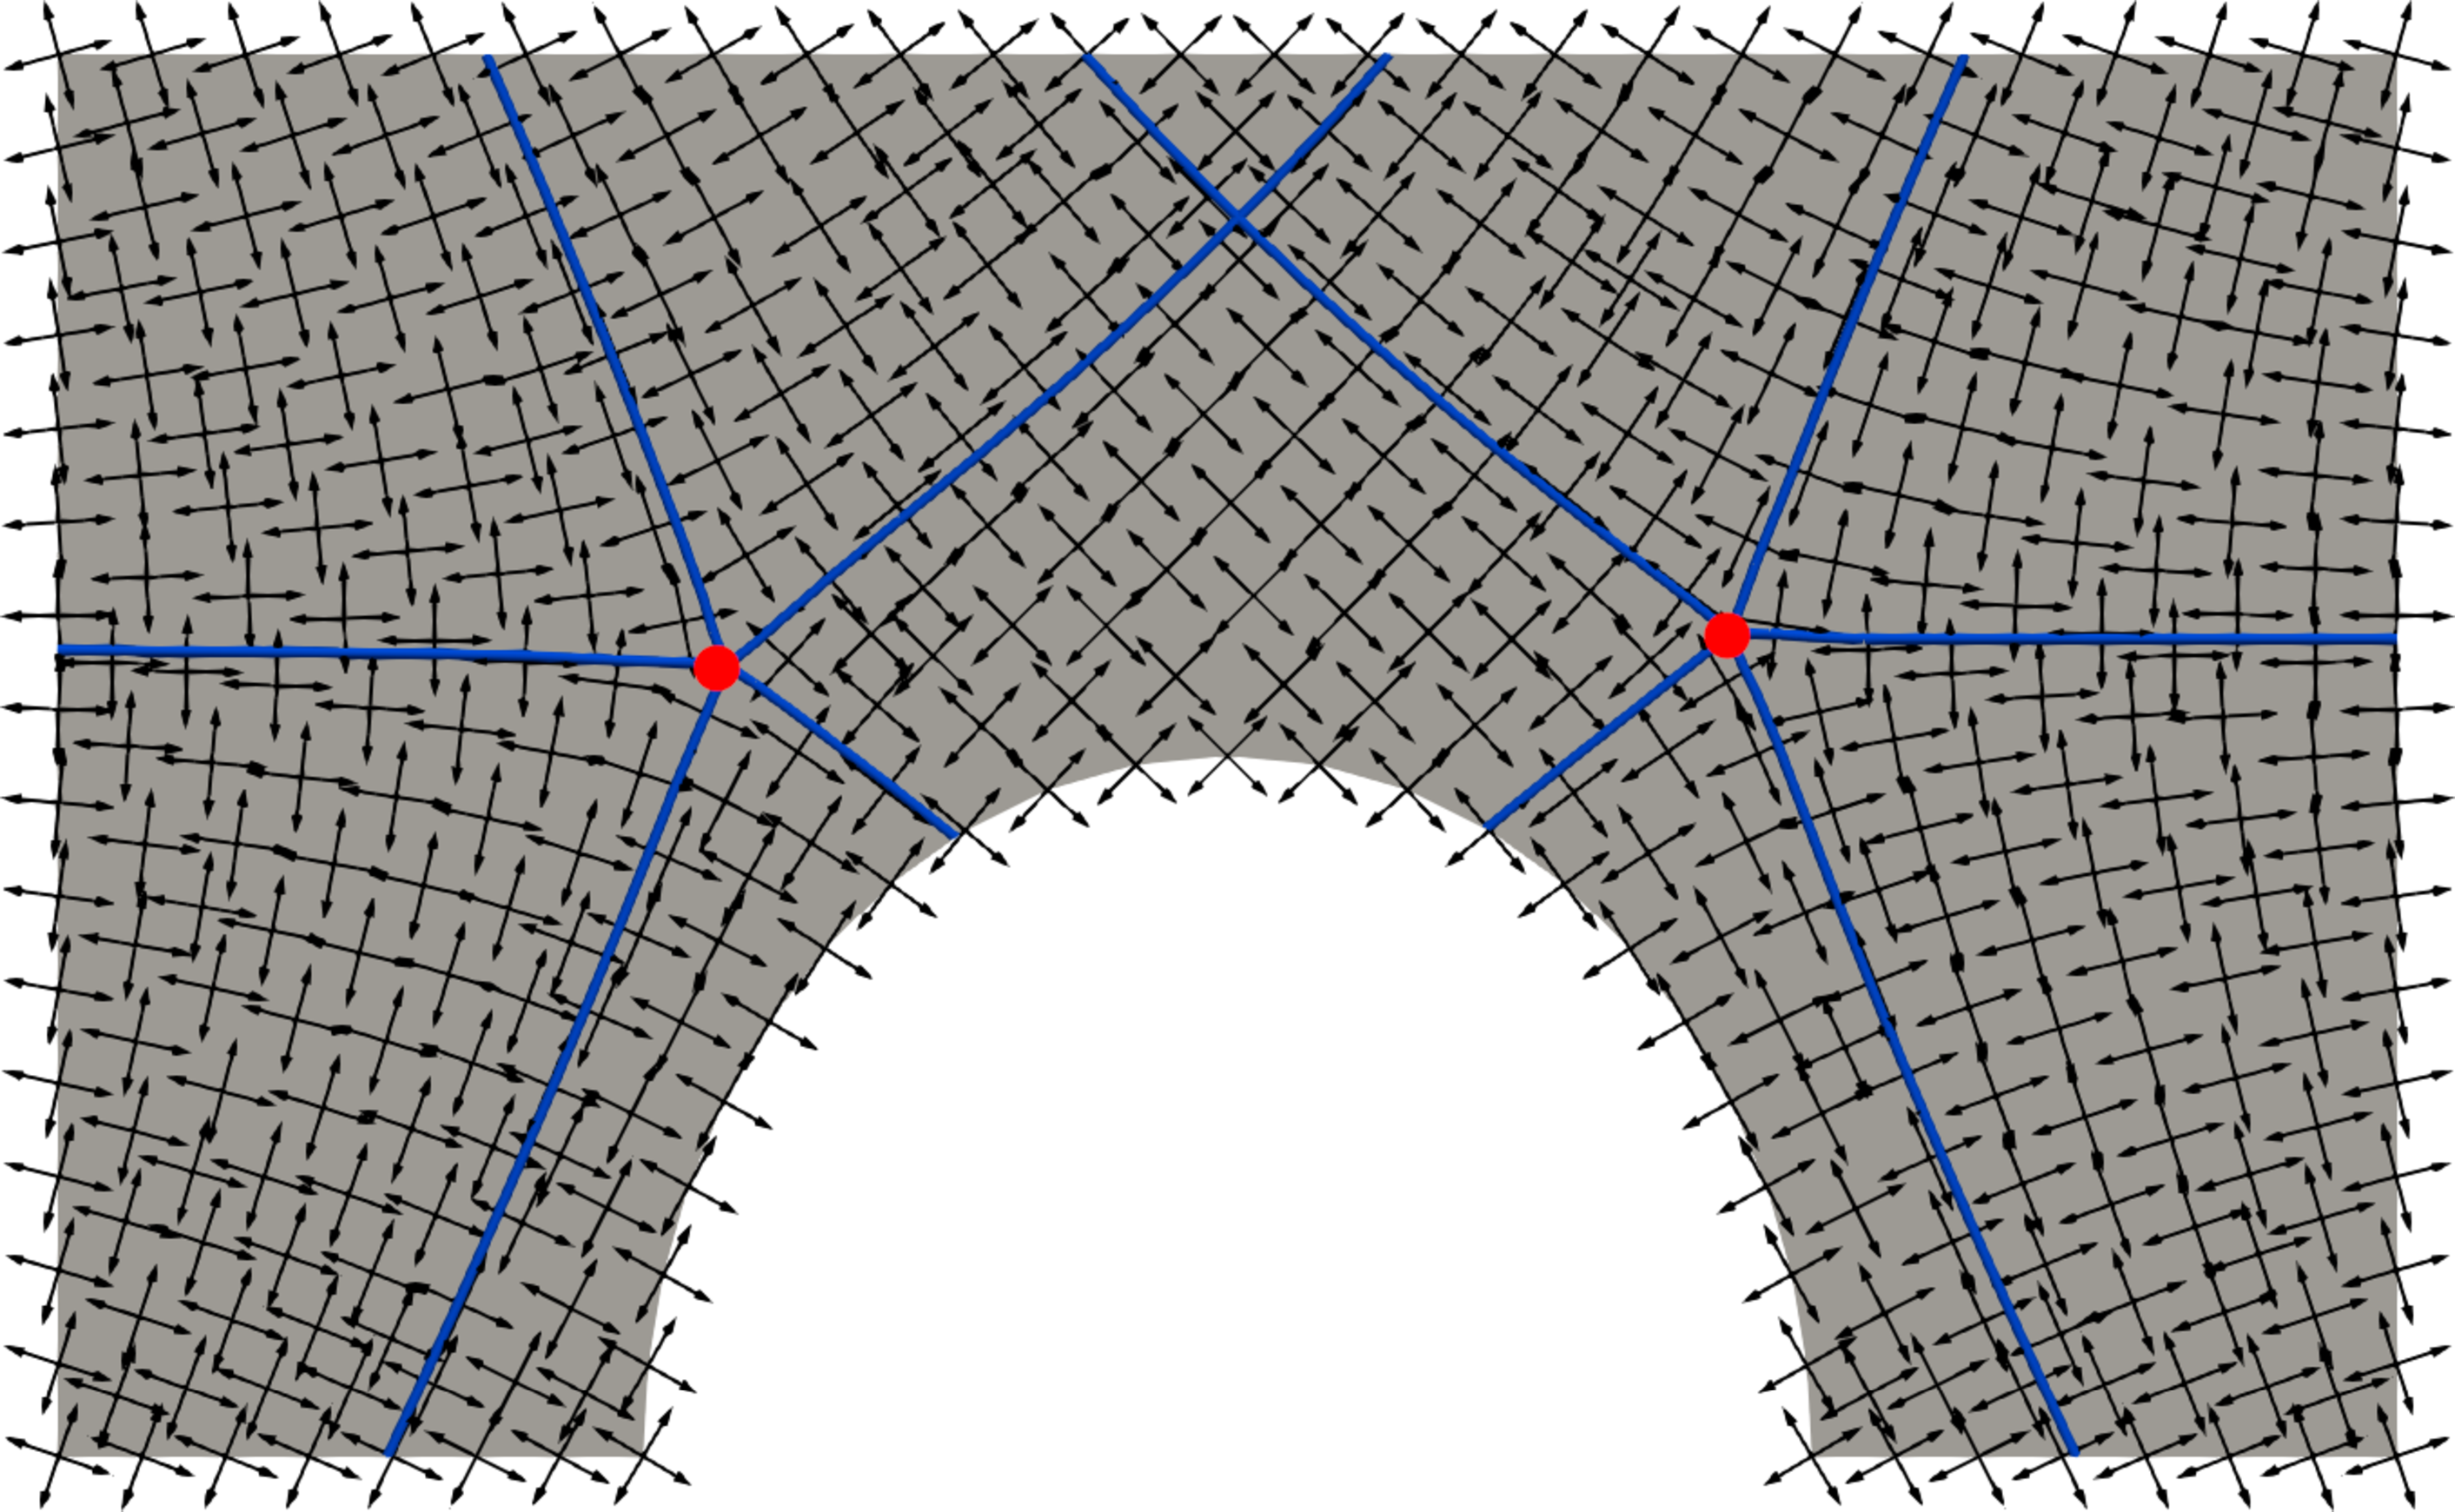
\includegraphics[width=\textwidth]{images/rect_demi_disc_first.pdf}
    \caption{Champ de croix initial avec deux points singuliers internes d'indice $1/4$.}
    \label{fig:rect_demi_disc_first}
\end{subfigure}
\\[0.46cm]
\begin{subfigure}{0.58\textwidth}
    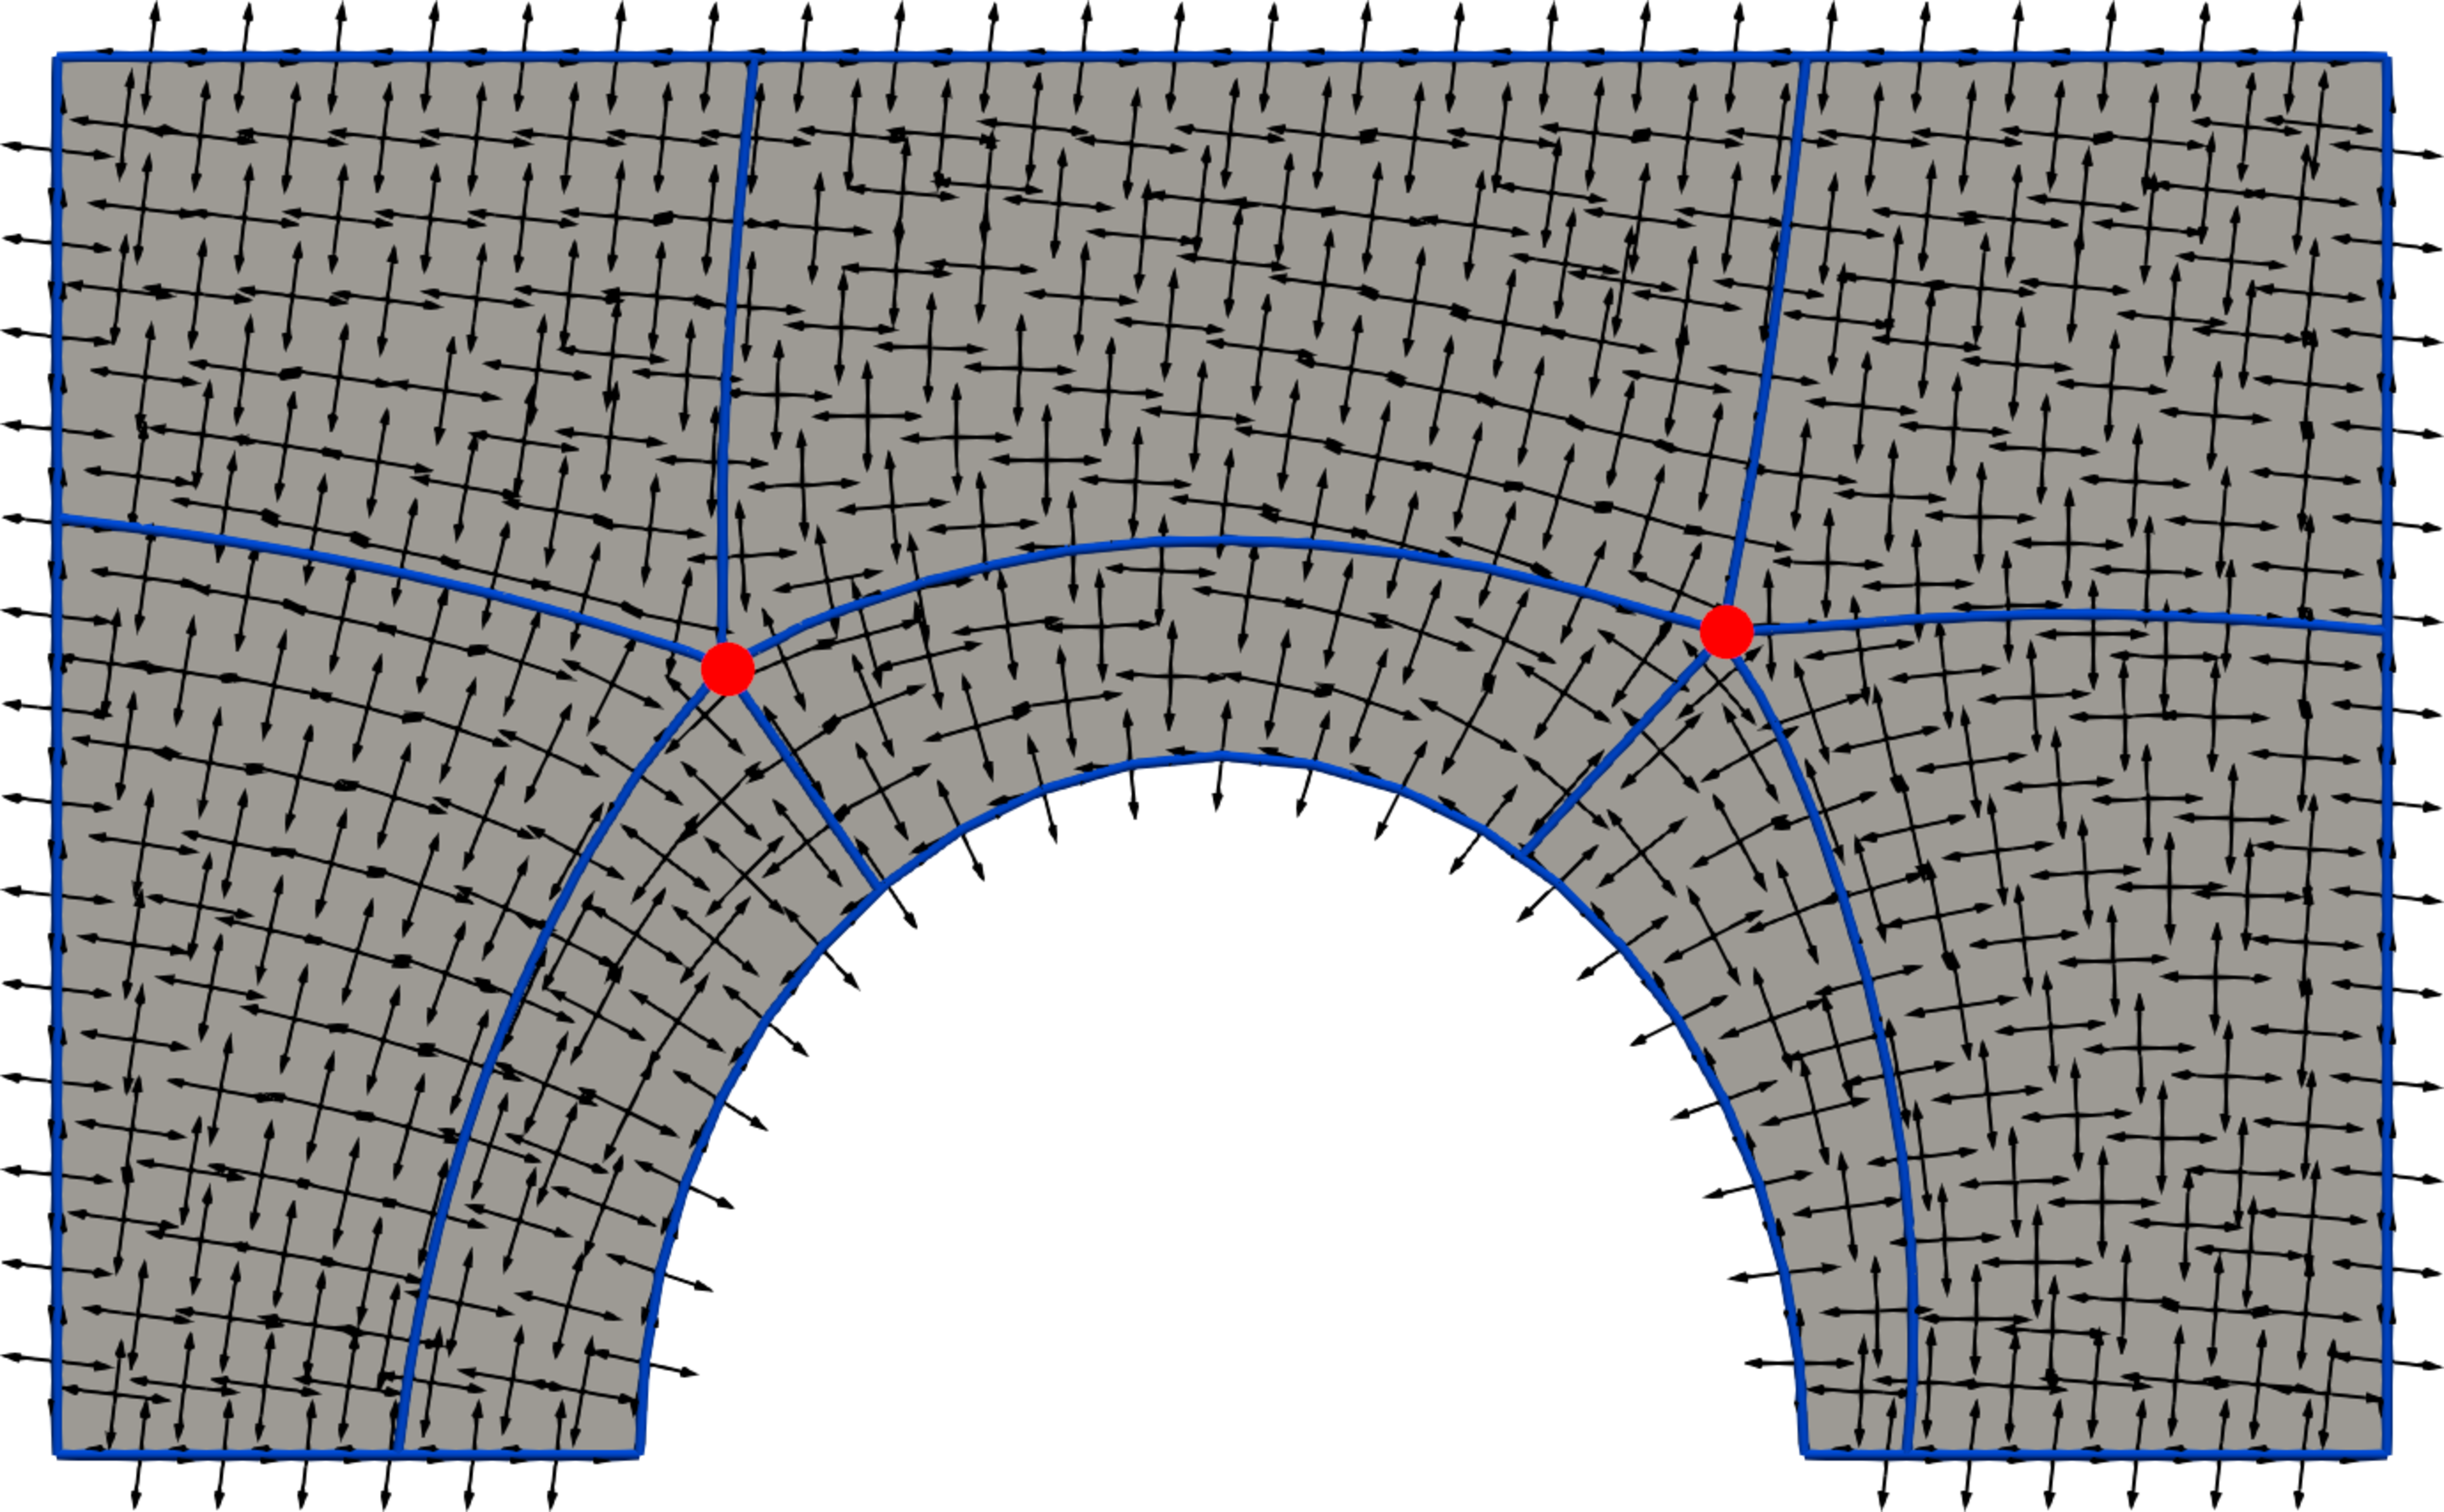
\includegraphics[width=\textwidth]{images/rect_demi_disc_second.pdf}
    \caption{Alignement du champ de croix initial sur le bord du domaine et partitionnement du domaine.}
    \label{fig:rect_demi_disc_second}
\end{subfigure}
\\[0.46cm]
\begin{subfigure}{0.58\textwidth}
    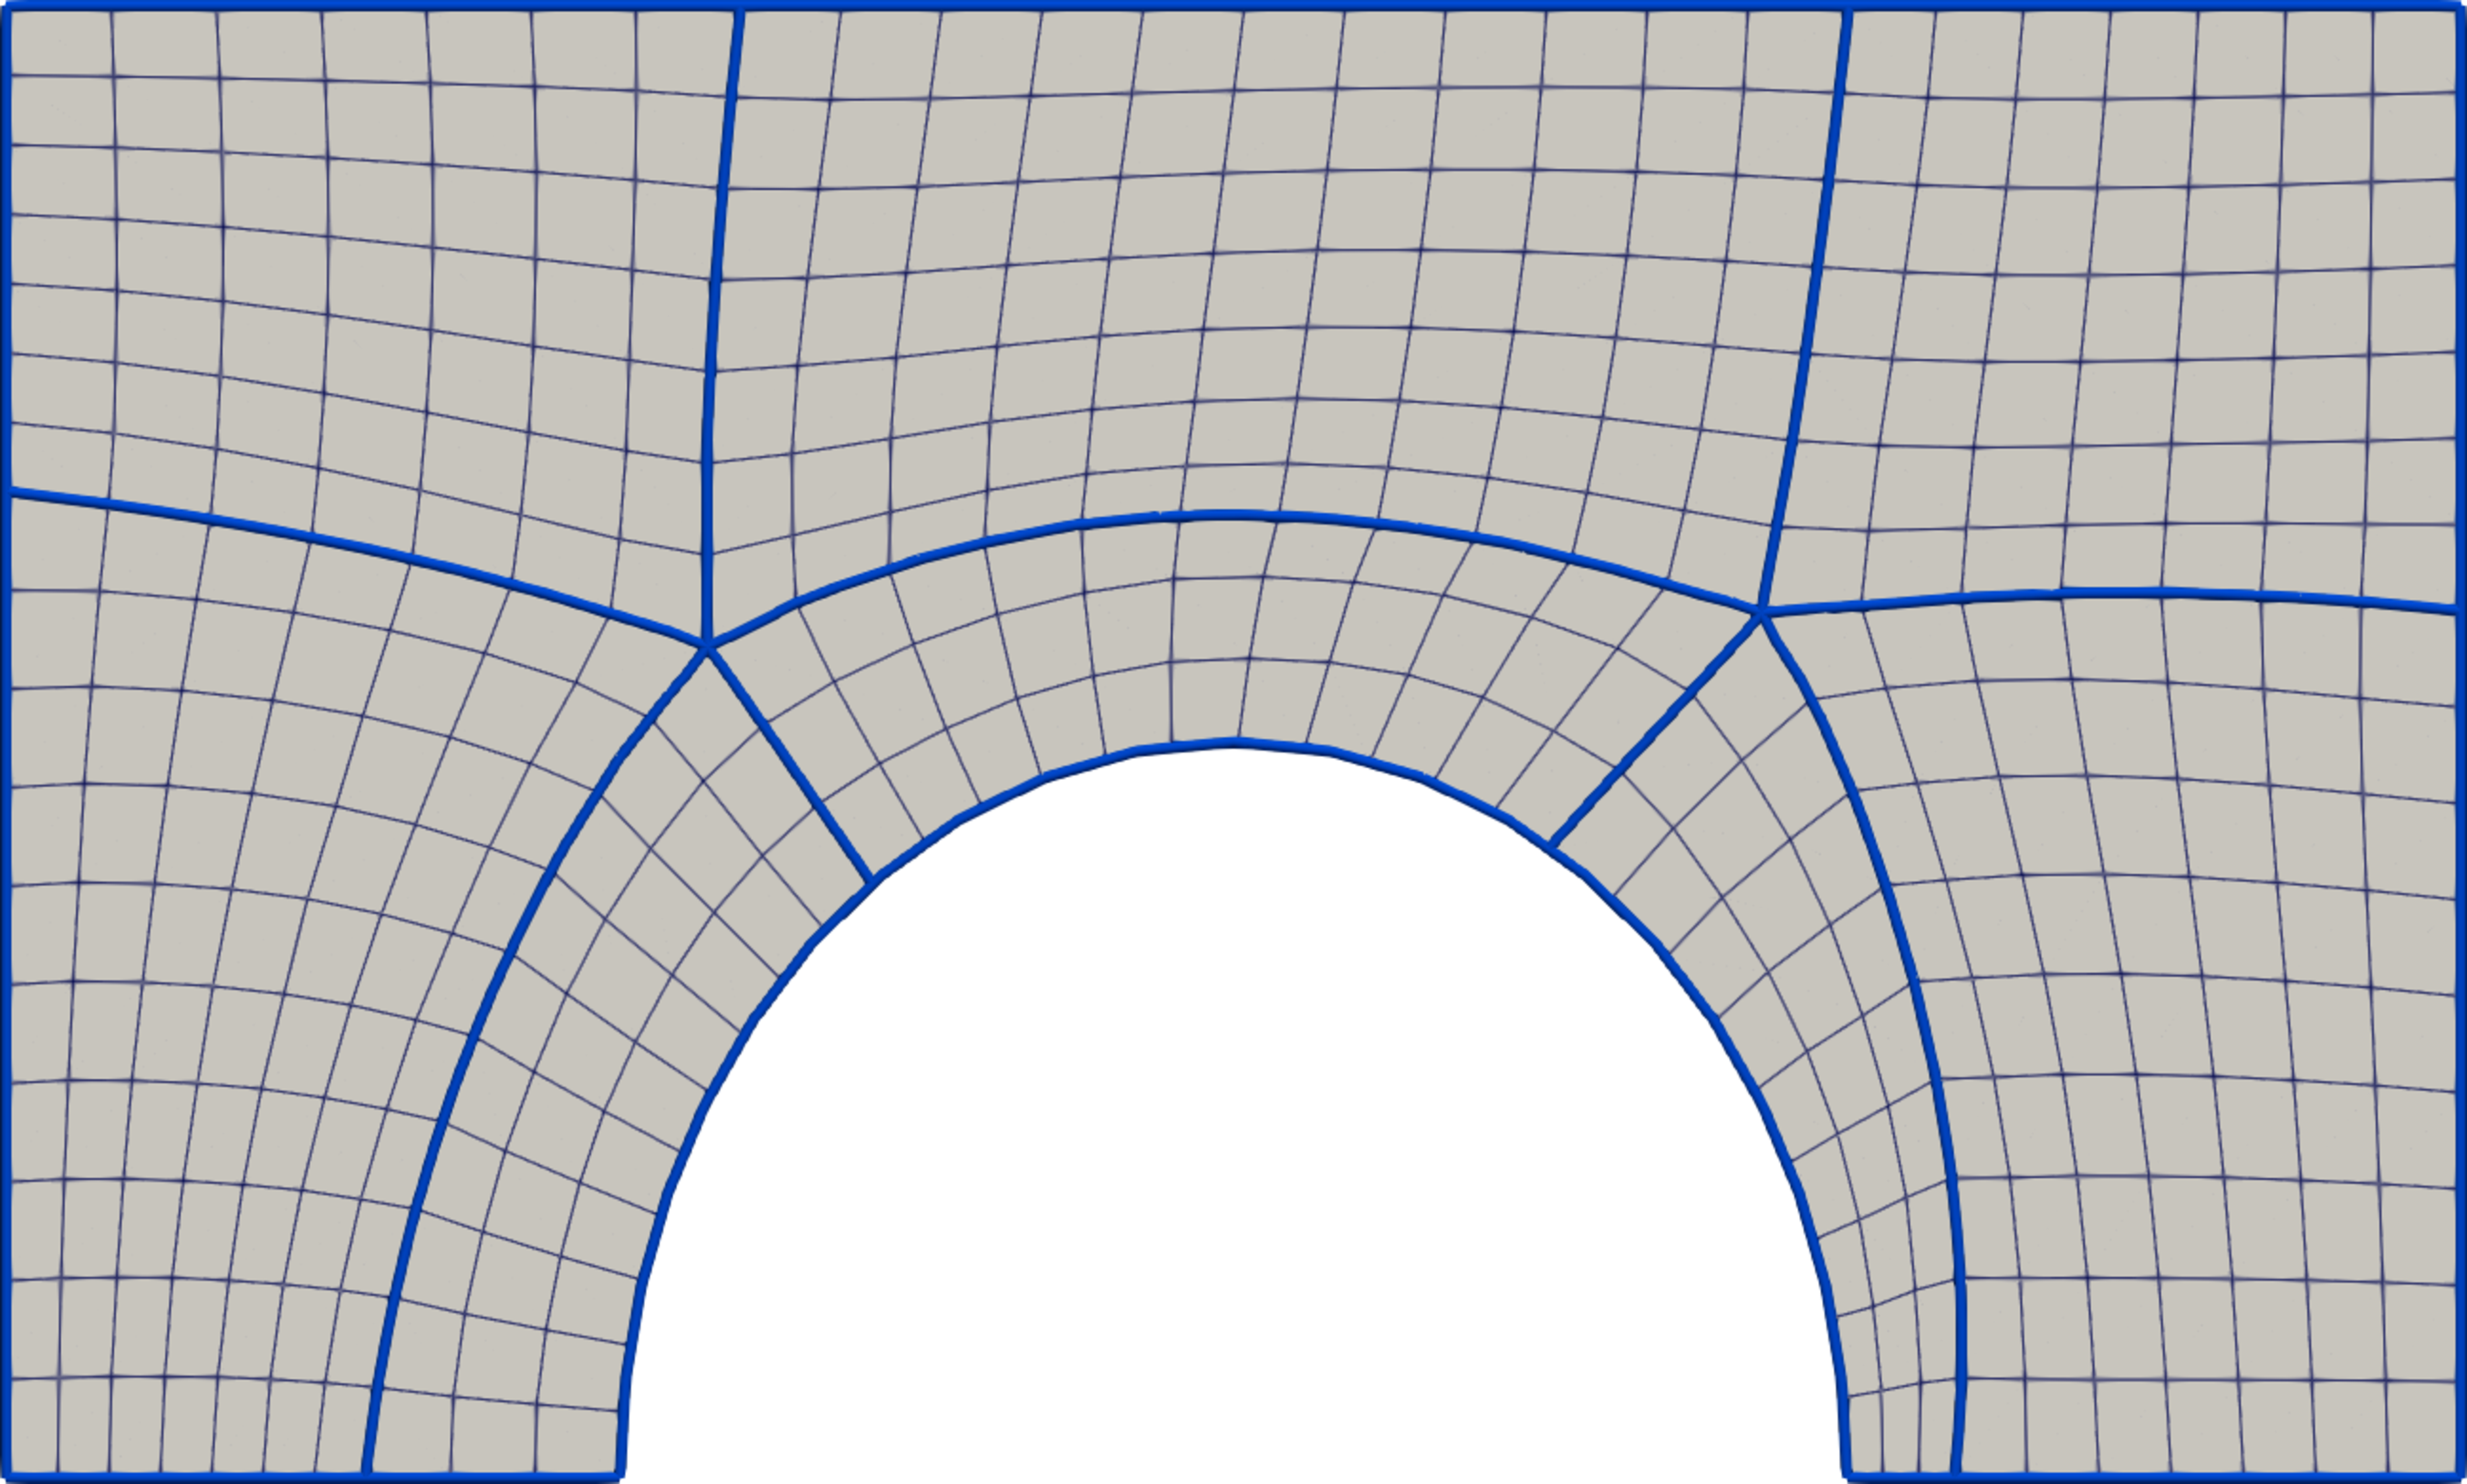
\includegraphics[width=\textwidth]{images/rect_demi_disc_third.pdf}
    \caption{Maillage quadilatéral du domaine présentant un quadrangle dégénéré.}
    \label{fig:rect_demi_disc_third}
\end{subfigure}
\caption{Une autre illustration de l'opération d'alignement à partir du champ d'angle donné.}
\label{fig:rect_demi_disc}
\end{figure}

\paragraph{Domaines non-simplement connexes:}
Nous supposons maintenant que $\Omega$ est un domaine non-simplement connexe. Autrement dit sa frontière $\partial\Omega$ peut potentiellement être constitué de plusieurs composantes connexes. On a donc $\partial\Omega=\cup_i\Gamma_i$, où $\Gamma_i,~i\in\llbracket 0, n_b-1\rrbracket$ désigne les composantes connexes de $\partial\Omega$ et $n_b$ le nombre de composantes connexes de $\partial\Omega$. Pour tout $i\in\llbracket0, n_b-1\rrbracket$, on note $\gamma_i$ la paramétrisation de $\Gamma_i$ sur $[0, 1]$ dans le sens positif. Soit $\bar{u}$ un champ de croix presque-$\mathcal{C}^1$ défini sur $\Omega$ et non-nécessairement aligné sur le bord de $\Omega$ tel que pour tout point $p\in\mathcal{S}_{\bar{u}}\backslash\partial\Omega$, $id_{\bar{u}}(p)=k/4$, avec $k\in\mathbb{Z}$ et $k\leq 1$. On suppose de plus que $0\leq Card(\mathcal{S}_{\bar{u}})+Card(\mathcal{B})< \infty$. En appliquant le processus présenté dans la partie précédente, la condition \eqref{eqn:principe_hypothese_u} devient:

\begin{equation}
    \sum_{i=0}^{n_b-1}\left(\theta_{\bar{u}}^{\gamma_i}(1)-\theta_{\bar{u}}^{\gamma_i}(0)\right)=2\pi\chi(\Omega)-2\pi\sum_{p\in\mathcal{B}}I_p.
    \label{eqn:principe_hypothese_u_prime}
\end{equation}
Cependant, cette condition ne permet pas de garantir que, pour tout $i\in\llbracket0, n_b-1\rrbracket$, $\phi(\gamma_i(1))-\phi(\gamma_i(0))=0$, ce qui est essentiel pour s'assurer que pour tout $p\in\partial \Omega$, $id_{\bar{v}}(p)= I_p$. C'est notamment ce qu'on observe sur l'exemple de la figure \ref{fig:carre_demi_disc_vide_mauvais}. Sur cet exemple, le champ de croix initial vérifie la condition \eqref{eqn:principe_hypothese_u_prime}. Elle contient deux points singuliers internes, chacun ayant un indice de $-1/4$. L'ensemble $\mathcal{B}$ se compose, d'une part, des quatre coins du bord carré où chaque coin a un paramètre $I_p$ fixé à $1/4$, et d'autre part, des deux coins du demi-disque où chaque coin a un paramètre $I_p$ fixé à $-1/4$. Le champ d'alignement est calculé avec l'équation \eqref{eqn:first_phi_computation}, puis le champ de croix $\bar{v}$ est construit. On observe clairement que $\bar{v}$ est bien aligné avec le bord du domaine et conserve les singularités internes du champ de croix initial. Cependant, on remarque l'apparition de singularités de bord dans le champ de croix $\bar{v}$. En appliquant l'algorithme de partitionnement \ref{alg:algo_main} sur $\bar{v}$, le partitionnement obtenu présente des régions à quatre côtés (figure \ref{fig:carre_demi_disc_vide_mauvais_second}) mais, la présence de points singuliers de bord non contrôlés (en termes de positionnement et d'indice) conduit à un maillage quadrilatéral comportant des quadrangles dégénérés (figure \ref{fig:carre_demi_disc_vide_mauvais_third}).

\begin{figure}[!h]
\centering
\begin{subfigure}{0.495\textwidth}
    \includegraphics[width=\textwidth]{images/carre_demi_disc_vide_mauvais_first.pdf}
    \caption{Champ de croix initial avec deux points singuliers internes, chacun d'indice $1/4$ et vérifiant l'équation \ref{eqn:principe_hypothese_u_prime}.}
    \label{fig:carre_demi_disc_vide_mauvais_first}
\end{subfigure}
\hfill
\begin{subfigure}{0.495\textwidth}
    \includegraphics[width=\textwidth]{images/carre_demi_disc_vide_mauvais_second.pdf}
    \caption{Alignement du champ de croix initial sur le bord du domaine et partitionnement du domaine.}
    \label{fig:carre_demi_disc_vide_mauvais_second}
\end{subfigure}
\\[0.2cm]
\begin{subfigure}{0.5\textwidth}
    \includegraphics[width=\textwidth]{images/carre_demi_disc_vide_mauvais_third.pdf}
    \caption{Maillage quadilatéral du domaine présentant des quadrangles dégénérés.}
    \label{fig:carre_demi_disc_vide_mauvais_third}
\end{subfigure}
\caption{Illustration de l'opération d'alignement sur un domaine non-simplement connexe à partir d'un champ de croix vérifiant la condition \eqref{eqn:principe_hypothese_u_prime}.}
\label{fig:carre_demi_disc_vide_mauvais}
\end{figure}
Pour surmonter cette limitation, nous modifions la conditions à imposer sur le champ de croix initial $\bar{u}$ de la manière suivante:
\begin{equation}
    \left\{
    \begin{array}{lcll}
    \theta_{\bar{u}}^{\gamma_0}(1)-\theta_{\bar{u}}^{\gamma_0}(0)&=&2\pi-2\pi\displaystyle\sum_{p\in\mathcal{B}\cap\Gamma_0}I_p&\mbox{ sur }\Gamma_0\\\\
    \theta_{\bar{u}}^{\gamma_i}(1)-\theta_{\bar{u}}^{\gamma_i}(0)&=&-2\pi-2\pi\displaystyle\sum_{p\in\mathcal{B}\cap\Gamma_i}I_p&\mbox{ sur }\Gamma_i,~\forall i\in\llbracket 1, n_b-1\rrbracket.
    \end{array}
    \right.
    \label{eqn:principe_hypothese_u_second}
\end{equation}
où $\Gamma_0$ désigne le bord extérieur de $\Omega$. En supposant que le champ de croix $\bar{u}$ vérifie cette condition, la condition de bord de l'équation \eqref{eqn:principe_def_phi} devient:
$$
\phi(\gamma_i(t))=\theta_{\bar{n}}^{\gamma_i}(t)+\mathcal{I}(t)-\theta_{\bar{u}}^{\gamma_i}(t) \mbox{ sur } \gamma_i^{-1}(\Gamma_i\backslash(\mathcal{B}\cup\mathcal{S}_{\bar{u}})),~\forall i\in\llbracket 0, n_b-1\rrbracket.
$$
\begin{remark}
    On montre (voir le Théorème \ref{thm:theorem3}) que le champ de croix $\bar{v}$ (résultant de l'opération d'alignement) est aligné par rapport à $\partial\Omega$. De plus pour tout $p\in\Omega\backslash\partial\Omega$, $id_{\bar{v}}(p)=id_{\bar{u}}(p)$ et pour tout $p\in\partial\Omega$, $id_{\bar{v}}(p)=I_p$.
\end{remark}
La figure \ref{fig:carre_demi_disc_vide_bon} donne une illustration de la construction d'un maillage quadrilatéral sur un domaine non-simplement connexe à partir d'un champ de croix vérifiant la condition \ref{eqn:principe_hypothese_u_second}. La figure \ref{LS89} donne une représentation visuelle supplémentaire.

\begin{figure}[!h]
\centering
\begin{subfigure}{0.495\textwidth}
    \includegraphics[width=\textwidth]{images/carre_demi_disc_vide_bon_first.pdf}
    \caption{Champ de croix initial avec deux points singuliers internes, chacun d'indice $1/4$ et vérifiant l'équation \ref{eqn:principe_hypothese_u_second}.}
    \label{fig:carre_demi_disc_vide_bon_first}
\end{subfigure}
\hfill
\begin{subfigure}{0.495\textwidth}
    \includegraphics[width=\textwidth]{images/carre_demi_disc_vide_bon_second.pdf}
    \caption{Alignement du champ de croix initial sur le bord du domaine et partitionnement du domaine.}
    \label{fig:carre_demi_disc_vide_bon_second}
\end{subfigure}
\\[0.8cm]
\begin{subfigure}{0.5\textwidth}
    \includegraphics[width=\textwidth]{images/carre_demi_disc_vide_bon_third.pdf}
    \caption{Maillage quadilatéral du domaine.}
    \label{fig:carre_demi_disc_vide_bon_third}
\end{subfigure}
\caption{Illustration de l'opération d'alignement sur un domaine non-simplement connexe à partir d'un champ de croix vérifiant la condition \eqref{eqn:principe_hypothese_u_second}.}
\label{fig:carre_demi_disc_vide_bon}
\end{figure}

\paragraph{Correction d'un champ de croix ne vérifiant pas la condition \eqref{eqn:principe_hypothese_u_second}:} D'après nos observations expérimentales, alors qu'il est relativement aisé de construire des champs de croix conformes à la formule \eqref{eqn:principe_hypothese_u_prime}, la génération de champs de croix respectant la formule \eqref{eqn:principe_hypothese_u_second} de manière simple et efficiente s'avère plus complexe. Par exemple le champ de croix illustré sur la figure \ref{fig:carre_demi_disc_vide_mauvais_first} vérifie \eqref{eqn:principe_hypothese_u_prime} mais pas \eqref{eqn:principe_hypothese_u_second}). Face à cette problématique, nous proposons une solution alternative en introduisant un processus de correction visant à modifier un champ de croix existant, $\bar{u}$ (vérifiant \ref{eqn:principe_hypothese_u_prime}), de manière à ce qu'il respecte la condition \eqref{eqn:principe_hypothese_u_second}. Cette démarche implique l'identification d'un champ d'angle $\omega$ permettant de définir un champ de croix corrigé, $\bar{u}_c$, à travers l'expression $\bar{u}_c:=\mathbf{R}(\omega)\bar{u}$, satisfaisant ainsi :
\begin{equation}
    \left\{
    \begin{array}{lcll}
    \theta_{\bar{u}_c}^{\gamma_0}(1)-\theta_{\bar{u}_c}^{\gamma_0}(0)&=&2\pi-2\pi\displaystyle\sum_{p\in\mathcal{B}\cap\Gamma_0}I_p&\mbox{ sur }\Gamma_0\\\\
    \theta_{\bar{u}_c}^{\gamma_i}(1)-\theta_{\bar{u}_c}^{\gamma_i}(0)&=&-2\pi-2\pi\displaystyle\sum_{p\in\mathcal{B}\cap\Gamma_i}I_p&\mbox{ sur }\Gamma_i,~\forall i\in\llbracket 1, n_b-1\rrbracket.
    \end{array}
    \right.
\end{equation}
De ce fait, le champ de croix corrigé $\bar{u}_c$ répond à la condition \eqref{eqn:principe_hypothese_u_second}. En appliquant le processus d'alignement à $\bar{u}_c$ ainsi que l'algorithme de partitionnement au champ résultant, nous parvenons à générer un maillage quadrilatéral du domaine initial. La construction du champ d'angle $\omega$ peut être effectuée selon diverses méthodes. Selon la méthode choisie, elle peut influencer les points singuliers de $\bar{u}$ et de l'ensemble $\mathcal{B}$ dans le maillage final. Nous reviendrons sur sa construction dans les parties suivantes (voir la section \ref{sec:discussion}).  L'algorithme \ref{alg:algo_non_simply_connected} résume la méthode de génération de maillage sur un domaine non-simplement connexe.

\vspace{0.5cm}
\begin{algorithm}[H]
\label{alg:algo_non_simply_connected}
\SetKwInOut{Input}{Entrée}
\SetKwInOut{Output}{Sortie}
\Input{$\Omega$ un domaine borné et fermé, champ de croix $\bar{u}$ défini sur $\Omega$, ensemble $\mathcal{B}$, paramètre $I_p$ pour tout $p\in\partial\Omega$.}
\Output{Partition de $\Omega$ en ensembles de régions.}
\vspace{0.2cm}
1.) Correction du champ de croix si nécessaire,\\\vspace{0.2cm}
1.) Calcul du champ d'alignement,\\\vspace{0.2cm}
2.) Calcul du champ de croix $\bar{v}$,\\\vspace{0.2cm}
3.) Application de l'algorithme \ref{alg:algo_main} au champ de croix $\bar{v}$.\\\vspace{0.2cm}
\caption{Algorithme de partitionnement pour un domaine non-simplement connexe basé sur un champ de croix non aligné}
\end{algorithm}
\vspace{0.5cm}

\begin{figure}[!h]
\centering
\includegraphics[scale=0.5]{images/LS89_bis.pdf}
\caption{Maillage du LS89 blade (géométrie détaillée dans \cite{gourdain2010advanced}).}
\label{LS89}
\end{figure}

\subsection{Etude de la méthode}
\label{subsec:etude_de_la_methode}
Dans la section précédente, nous avons exposé des algorithmes qui, sous certaines conditions, permettent de subdiviser un domaine en régions à quatres côtés. Dans cette partie, nous allons présenter plusieurs résultats visant à garantir l'efficacité de ces méthodes. Commençons par le cas où le champ de croix est aligné avec le bord du domaine. Nous avons le résultat suivant:
\begin{theorem}
\label{thm:theorem1}
Soit $\Omega$ un domaine borné et fermé dans $\mathbb{R}^2$ avec une frontière régulière par morceau et soit $\bar{u}$ un champ de croix presque-$\mathcal{C}^1$ aligné avec $\partial\Omega$ tel que $0<Card(\mathcal{S}_{\bar{u}})<\infty$ et pour tout $p\in\Omega$, $id_{\bar{u}}(p)=k/4$ où $k\in\mathbb{Z}$ et $k\leq 1$. Si l'algorithme de partitionnement \ref{alg:algo_main} appliqué à $\bar{u}$ converge alors le partitionnement résultant est une décomposition de $\Omega$ en régions à quatre côtés.
\end{theorem}

\begin{proof}
Selon les propositions \ref{prop:stream_from_interior_sing} et \ref{prop:stream_from_bord_sing}, chaque point singulier de $u$ donne lieu à un nombre fini de séparatrices. Étant donné que par hypothèse ces séparatrices ne convergent pas vers des cycles limites, elles doivent soit se terminer en un point singulier, soit intersecter la frontière de $\Omega$. En conséquence, les séparatrices de $\bar{u}$ divisent $\Omega$ en régions qui ne contiennent aucun point singulier et qui sont délimitées par des séparatrices.

Soit $\mathcal{R}$ l'une de ces régions. Selon le Théorème de Poincaré-Hopf, on a $\chi(\mathcal{R})=\sum_{i=1}^{n_c} id_{\bar{u}}(c_i)$, où $(c_i)_{i\in\llbracket1,n_c\rrbracket}$ désigne les coins de $\mathcal{R}$ (c'est à dire les points d'intersections des séparatrices formant la région $\mathcal{R}$) et $n_c$ est le nombre de coins. $\chi(\mathcal{R})\geq0$ car, d'après la proposition \ref{prop:loveprop}, nous avons $id_{\bar{u}}(c_i)=1/4>0$ pour chaque coin $c_i$ de $\mathcal{R}$. De plus, on sait que $\chi(\mathcal{R}) = 2 - 2g - b$, où $g$ représente le genre de $\mathcal{R}$ et $b$ le nombre de composantes connexes de $\partial\mathcal{R}$ (détail en Annexe). Comme $\mathcal{R}$ est une partie du plan, on a $g = 0$, ce qui implique que $\chi(\mathcal{R})\in\{0, 1\}$.
\begin{itemize}
\item $\chi(\mathcal{R})=0$: dans ce cas on a $n_c=0$ et $\mathcal{R}=\Omega$. Cela mène à une contradiction puisque, selon les hypothèses du théorème on a $Card(\mathcal{S}_{\bar{u}})>0$.
\item $\chi(\mathcal{R})=1$: cela implique que :
$$1=\sum_{i=1}^{n_c}id_u(c_i)=\sum_{i=1}^{n_c}\frac{1}{4}\Longrightarrow n_c=4.$$
Ainsi, $\mathcal{R}$ est une région à quatre côtés.
\end{itemize}
\end{proof}

\paragraph{\'Etude de l'opération d'alignement}

Soit $\Omega$ un domaine fermé et borné dans $\mathbb{R}^2$ avec une frontière lisse par morceaux. Supposons dans un premier temps que $\Omega$ est simplement connexe. Soit $\mathcal{B}\subset\partial\Omega$ un ensemble de point isolé de $\partial\Omega$ et $I_p$ un paramètre associé à chaque point $p\in\Omega$ tel que:
\begin{equation}
I_p=
\left\{
\begin{array}{ll}
\displaystyle\frac{k}{4}\mbox{ avec }k\in\mathbb{Z}^*\mbox{ et }k\leq 1& \mbox{ si } p\in\mathcal{B}\\[0.5cm]
0& \mbox{ sinon }
\end{array}
\right.
\label{eqn:etude_def_I}
\end{equation}
Soit $\bar{u}$ un champ de croix presque-$\mathcal{C}^1$ défini sur $\Omega$, non nécessairement aligné sur $\partial\Omega$, tel que pour tout point $p\in\mathcal{S}_{\bar{u}}\backslash\partial\Omega$, $id_{\bar{u}}(p)=k/4$, avec $k\in\mathbb{Z}$ et $k\leq 1$. On suppose de plus que $0< Card(\mathcal{S}_{\bar{u}})+Card(\mathcal{B})< \infty$ et qu'il existe $\theta_{\bar{u}}^\gamma$ un relèvement continu de $\bar{u}$ le long de $\gamma$ tel que:
\begin{equation}
    \label{eqn:etude_hypothese_u}
    \theta_{\bar{u}}^\gamma(1)-\theta_{\bar{u}}^\gamma(0)=2\pi\chi(\Omega)-2\pi\sum_{p\in\mathcal{B}}I_p.
\end{equation}
où $\gamma$ est une paramétrisation sur $[0, 1]$ de $\partial\Omega$ orientée positivement et vérifiant $\gamma(0)=\gamma(1)\notin\mathcal{B}\cup\mathcal{S}_{\bar{n}}\cup\mathcal{S}_{\bar{u}}$.
Soit $\phi$, la fonction définie par l'équation \eqref{eqn:principe_def_phi}. Nous avons alors le lemme suivant:

\begin{lemma}
    \label{lem:marvelous_lemma}
    $\phi(\gamma(1))-\phi(\gamma(0))=0$.
\end{lemma}
\begin{proof}
    $$
    \begin{array}{lcl}
        \phi(\gamma(1))-\phi(\gamma(0))&=&\theta^\gamma_{\bar{n}}(1)+\mathcal{I}(1)-\theta_{\bar{u}}(\gamma(1))-(\theta^\gamma_{\bar{n}}(0)+\mathcal{I}(0)-\theta_{\bar{u}}^\gamma(0))\\\\
        &=&(\theta^\gamma_{\bar{n}}(1)-\theta_{\bar{n}}^\gamma(0))+(\mathcal{I}(1)-\mathcal{I}(0))-(\theta_{\bar{u}}^\gamma(1)-\theta_{\bar{u}}^\gamma(0)).
    \end{array}
    $$
    En posant $\gamma^{-1}(\mathcal{B}\cup\mathcal{S}_{\bar{n}})=\{t_1,\dots,t_{n_t}\}$ avec $n_t\in\mathbb{N}^*$ et $t_1<\dots<t_{n_t}$, on a:
    $$
    \begin{array}{lcl}
        \theta_{\bar{n}}^\gamma(1)-\theta^\gamma_{\bar{n}}(0)&=&\theta_{\bar{n}}^\gamma(t_1^-)-\theta_{\bar{n}}^\gamma(0)+\displaystyle\sum_{i=2}^{n_t}\left(\theta_{\bar{n}}^\gamma(t_i^-)-\theta_{\bar{n}}^\gamma(t_{i-1}^+)\right)+\theta_{\bar{n}}^\gamma(0)\\[0.7cm]
        &&+\theta_{\bar{n}}^\gamma(1)-\theta_{\bar{n}}^\gamma(t_{n_t}^-)+\displaystyle\sum_{i=1}^{n_t}\left(\theta_{\bar{n}}^\gamma(t_i^+)-\theta_{\bar{n}}^\gamma(t_i^-)\right)-\theta_{\bar{n}}^\gamma(0)\\[0.7cm]
        &=&\displaystyle\int_0^1d\theta_{\bar{n}}^\gamma+\displaystyle\sum_{i=1}^{n_t}\left(\theta_{\bar{n}}^\gamma(t_i^+)-\theta_{\bar{n}}^\gamma(t_i^-)\right)\\[0.7cm]
        \theta_{\bar{n}}^\gamma(1)-\theta^\gamma_{\bar{n}}(0)&=&\displaystyle\int_0^1d\theta_{\bar{n}}^\gamma+\displaystyle\sum_{s\in\gamma^{-1}(\mathcal{B}\cup\mathcal{S}_{\bar{n}})}\left(\theta_{\bar{n}}^\gamma(s^+)-\theta_{\bar{n}}^\gamma(s^-)\right).
    \end{array}
    $$
    Remarquons aussi que puisque $\mathcal{I}(0)=0$, on a:
    $$
    \mathcal{I}(1)-\mathcal{I}(0)=\sum_{s\in\gamma^{-1}(\mathcal{B}\cup\mathcal{S}_{\bar{n}})}\left[\left(\pi-\widehat{\gamma(s)}-2\pi I_{\gamma(s)}\right)-\left(\theta^{\gamma}_{\bar{n}}(s^+)-\theta^{\gamma}_{\bar{n}}(s^-)\right)\right].
    $$
    Il vient alors que:
    $$
    \phi(\gamma(1))-\phi(\gamma(0))=\displaystyle\int_0^1d\theta_{\bar{n}}^\gamma+\sum_{s\in\gamma^{-1}(\mathcal{B}\cup\mathcal{S}_{\bar{n}})}\left(\pi-\widehat{\gamma(s)}-2\pi I_{\gamma(s)}\right)-(\theta_{\bar{u}}^\gamma(1)-\theta_{\bar{u}}^\gamma(0)).
    $$
    Autrement dit,
    $$
    \begin{array}{lcl}
        \phi(\gamma(1))-\phi(\gamma(0))&=&\displaystyle\sum_{i=1}^{n_t}\int_{t_i}^{t_{i+1}}d\theta_{\bar{n}}^\gamma+\sum_{s\in\gamma^{-1}(\mathcal{B})}\left(\pi-\widehat{\gamma(s)}\right)\\[0.7cm]
        &&-\displaystyle\left(\sum_{s\in\gamma^{-1}(\mathcal{B}\cup\mathcal{S}_{\bar{n}})}2\pi I_{\gamma(s)}+(\theta_{\bar{u}}^\gamma(1)-\theta_{\bar{u}}^\gamma(0))\right),
    \end{array}
    $$
    où on a posé $t_{n_t+1}:=t_1$. D'après le théorème des tangentes tournantes \cite{hopf1935drehung, rotskoff2010gauss}, on sait que :
    $$
    \displaystyle\sum_{i=1}^{n_t}\left(\theta_{\bar{n}}^\gamma(t_{i+1})-\theta_{\bar{n}}^\gamma(t_i)\right)+\sum_{s\in\gamma^{-1}(\mathcal{B}\cup\mathcal{S}_{\bar{n}})}\left(\pi-\widehat{\gamma(s)}\right)=2\pi.
    $$
    On obtient alors en utilisant la condition \eqref{eqn:etude_hypothese_u}
    $$
    \phi(\gamma(1))-\phi(\gamma(0))=2\pi-2\pi\chi(\Omega).
    $$
    Autrement dit,
    $$
    \phi(\gamma(1))-\phi(\gamma(0))=0.
    $$
\end{proof}
L'opération d'alignement consiste à calculer le champ de croix $\bar{v}$ défini pour tout $p\in\Omega$ par:
\begin{equation}
\bar{v}(p)=
\left\{
\begin{array}{ll}
\mathbf{R}(\phi(p))\bar{u}(p) & \mbox{ si } p\in\Omega\backslash(\mathcal{B}\cup\mathcal{S}_{\bar{n}}\cup\mathcal{S}_{\bar{u}}),\\[0.5cm]
\bar{n}(p) & \mbox{ si } p\in(\mathcal{S}_{\bar{u}}\cap\partial\Omega)\backslash(\mathcal{B}\cup\mathcal{S}_{\bar{n}}),\\[0.5cm]
0 & \mbox{ si } p\in\mathcal{B}\cup\mathcal{S}_{\bar{n}}.
\end{array}
\right.
\label{eqn:etude_def_v}
\end{equation}
Nous avons alors le théorème suivant:
\begin{theorem}
\label{thm:theorem2}
Le champ de croix $\bar{v}$ est presque-$\mathcal{C}^1$ sur $\Omega$ et aligné avec $\partial\Omega$. De plus, pour tout $p\in\Omega$, on a:
\begin{equation}
id_{\bar{v}}(p)=
\left\{
\begin{array}{ll}
    id_{\bar{u}}(p) & \mbox{ si } p\in\Omega\backslash\partial\Omega,\\\\
    I_p & \mbox{ sinon }.
\end{array}
\right.
\end{equation}
\end{theorem}

\begin{proof}
    Du fait que la fonction $\phi$ définie par l'équation \eqref{eqn:principe_def_phi} est de classe $\mathcal{C}^1$ sur $\Omega\backslash(\mathcal{B}\cup\mathcal{S}_{\bar{n}}\cup(\mathcal{S}_{\bar{u}}\cap\partial\Omega)))$, le champ $\bar{v}$ est presque-$\mathcal{C}^1$ sur $\Omega$. Cela découle immédiatement de la proposition \ref{prop:cont1}, étant donné que $\bar{u}$ est presque-$\mathcal{C}^1$ sur $\Omega$.

    De plus, $\bar{v}$ est aligné avec $\partial\Omega$. En effet, $\bar{v}(p)=0$ pour tout $p\in\mathcal{B}\cup\mathcal{S}_{\bar{n}}$ et $\bar{v}(p)=\bar{n}(p)$ pour tout $p\in(\mathcal{S}_{\bar{u}}\cap\partial\Omega)\backslash(\mathcal{B}\cup\mathcal{S}_{\bar{n}})$. Par ailleurs, pour tout $p\in\partial\Omega\backslash(\mathcal{B}\cup\mathcal{S}_{\bar{n}}\cup\mathcal{S}_{\bar{u}})$ on a:
    $$\theta_{\bar{v}}(\gamma(t_p))=\phi(\gamma(t_p))+\theta_{\bar{u}}^\gamma(t_p)+k\frac{\pi}{2}=\theta_{\bar{n}}^\gamma(t_p)+\mathcal{I}(t_p)-\theta_{\bar{u}}^\gamma(t_p)+\theta_{\bar{u}}^\gamma(t_p)+k\frac{\pi}{2},$$
    où $t_p\in[0,1]$ tel que $\gamma(t_p)=p$ et $k\in\mathbb{Z}$. Or pour tout $s\in\gamma^{-1}(\mathcal{B}\cup\mathcal{S}_{\bar{n}})\cap[0, t_p]$ on a:
    $$
    \lim\limits_{r\rightarrow s^+}\theta^{\gamma}_{\bar{n}}(r) - \lim\limits_{r\rightarrow s^-}\theta^{\gamma}_{\bar{n}}(r)\equiv(\pi-\widehat{\gamma(s)})\pmod{\frac{\pi}{2}}.
    $$
    Il vient alors que:
    $$
    \theta_{\bar{v}}(\gamma(t_p))=\theta_{\bar{n}}^{\gamma}(t_p)+\displaystyle\sum_{s\in\gamma^{-1}(\mathcal{B}\cup\mathcal{S}_{\bar{n}})}\left[\left(\pi-\widehat{\gamma(s)}-m_s\frac{\pi}{2}\right)-\left(\pi-\widehat{\gamma(s)}+k_s\frac{\pi}{2}\right)\right]\mathbb{1}_{[0, t_p]}(s)+k\frac{\pi}{2},
    $$
    où $k_s\in\mathbb{Z}$ et où on a posé $I_{\gamma(s)}=m_s/4$ avec $m_s\in\mathbb{Z}$ et $m_s\leq1$. Autrement dit, on a:
    $$
    \theta_{\bar{v}}(\gamma(t_p))=\theta_{\bar{n}}^\gamma(t_p)+\displaystyle\sum_{s\in\gamma^{-1}(\mathcal{B}\cup\mathcal{S}_{\bar{n}})}\left[-m_s\frac{\pi}{2}+k_s\frac{\pi}{2}\right]\mathbb{1}_{[0, t_p]}(s)+k\frac{\pi}{2},$$
    et donc:
    $$
    \theta_{\bar{v}}(\gamma(t_p))\equiv\theta_{\bar{n}}^\gamma(t_p)\pmod{\frac{\pi}{2}}.
    $$
    Ce qui implique que $\bar{v}(p)=\bar{n}(p)$. On conclut alors que $\bar{v}$ est aligné avec $\partial\Omega$.\\\\
    Nous calculons maintenant pour tout $p\in\Omega$, l'indice de $p$ dans le champ $\bar{v}$. Ainsi, on a:\\
    \begin{itemize}
        \item[$\bullet$] Si $p\in\Omega\backslash\partial\Omega$, $id_{\bar{v}}(p)=id_{\bar{u}}(p)$ selon la proposition \ref{prop:relation_u_Rthetau}, car la fonction $\phi$ définie par l'équation \eqref{eqn:principe_def_phi} est de classe $\mathcal{C}^1$ sur $\Omega\backslash\partial\Omega$.\\
        \item[$\bullet$] Si $p\in\partial\Omega\backslash\{\gamma(0)\}$ (sachant que $\gamma(0)=\gamma(1)$), on a:
        $$
        id^\partial_{\bar{v}}(p)=\frac{1}{2\pi}\left[\pi-\widehat{p}+\displaystyle\lim\limits_{s\rightarrow 0}\int_s^{1-s}d\theta_{\bar{v}}^{\mathcal{C}}\right]=\frac{1}{2\pi}\left(\pi-\widehat{p}+(\theta_{\bar{v}}^{\mathcal{C}}(1)-\theta_{\bar{v}}^{\mathcal{C}}(0))\right),
        $$
        où $\mathcal{C}$ est un lacet paramétré sur $[0, 1]$ tel que $\mathcal{C}(0)=p=\mathcal{C}(1)$ et les vecteurs $\mathcal{C}'(0)$ et $\mathcal{C}'(1)$ sont tangents à $\partial\Omega$. De plus, $\mathcal{C}$ n'englobe aucun autre point singulier de $\bar{u}$. Soit $t_p\in]0, 1[$ tel que $\gamma(t_p)=p$. On a:
        $$
        id^\partial_{\bar{v}}(p)=\frac{1}{2\pi}\left[\pi-\widehat{p}+\left(\theta_{\bar{v}}^\gamma(t_p^-)-\theta_{\bar{v}}^\gamma(t_p^+)\right)\right],
        $$
        où on a noté $\lim_{t\rightarrow t_p^+}\theta^\gamma_{\bar{v}}(t)=\theta^\gamma_{\bar{v}}(t_p^+)$ et $\lim_{t\rightarrow t_p^-}\theta^\gamma_{\bar{v}}(t)=\theta_{\bar{v}}^\gamma(t_p^-)$. Autrement dit, on a:
        $$
        \begin{array}{lcl}
        id^\partial_{\bar{v}}(p)&=&\displaystyle\frac{1}{2\pi}\left[\pi-\widehat{p}+\left(\phi(\gamma(t_p^-))+\theta_{\bar{u}}^\gamma(t_p^-)-\phi(\gamma(t_p^+))-\theta_{\bar{u}}^\gamma(t_p^+)\right)\right]\\\\
        &=&\displaystyle\frac{1}{2\pi}\left[\pi-\widehat{p}+\left(\theta_{\bar{n}}^\gamma(t_p^-)-\theta_{\bar{n}}^\gamma(t_p^+)\right)+\left(\mathcal{I}(t_p^-)-\mathcal{I}(t_p^+)\right)\right].
        \end{array}
        $$
        Remarquons que:
        \begin{eqnarray*}
            \mathcal{I}(t_p^+)-\mathcal{I}(t_p^-)&=&\sum_{s\in\gamma^{-1}(\mathcal{B}\cup\mathcal{S}_{\bar{n}})\cap[0, t_p]}\left[\left(\pi-\widehat{\gamma(s)}-2\pi I_{\gamma(s)}\right)-\left(\theta^{\gamma}_{\bar{n}}(s^+) - \theta^{\gamma}_{\bar{n}}(s^-)\right)\right]\\\\
            &&-\sum_{s\in\gamma^{-1}(\mathcal{B}\cup\mathcal{S}_{\bar{n}})\cap[0, t_p[}\left[\left(\pi-\widehat{\gamma(s)}-2\pi I_{\gamma(s)}\right)-\left(\theta^{\gamma}_{\bar{n}}(s^+) - \theta^{\gamma}_{\bar{n}}(s^-)\right)\right]\\\\
            &=&\left(\pi-\widehat{p}-2\pi I_p\right)-\left(\theta^{\gamma}_{\bar{n}}(t_p^+) - \theta^{\gamma}_{\bar{n}}(t_p^-)\right).
        \end{eqnarray*}
        Il vient alors que:
        \begin{eqnarray*}
        id^\partial_{\bar{v}}(p)&=&\displaystyle\frac{1}{2\pi}\left[\pi-\widehat{p}-\left(\theta^{\gamma}_{\bar{n}}(t_p^+) - \theta^{\gamma}_{\bar{n}}(t_p^-)\right)-\left(\pi-\widehat{p}-2\pi I_p\right)+\left(\theta^{\gamma}_{\bar{n}}(t_p^+) - \theta^{\gamma}_{\bar{n}}(t_p^-)\right)\right]\\\\
        &=&\displaystyle\frac{1}{2\pi}\left[\pi-\widehat{p}-\left(\pi-\widehat{p}-2\pi I_p\right)\right].
        \end{eqnarray*}
        Par conséquent, $id^\partial_{\bar{v}}(p)=I_p$.\\
        \item[$\bullet$] Supposons maintenant que $p=\gamma(0)=\gamma(1)$. Puisque $\bar{v}$ est aligné par rapport à $\partial\Omega$, en appliquant le théorème de Poincaré-Hopf à $\bar{v}$, on obtient :
        $$
        \sum_{q\in\Omega} id_{\bar{v}}(q)+\sum_{q\in\partial\Omega\backslash\partial\Omega} id^\partial_{\bar{v}}(q)=\chi(\Omega).
        $$
        % BIEN SUR ICI ON PEUT DIRE QUE LA SOMME DES ID_V= SOMME DES ID_U MAIS CE N'EST PAS DE CA ON A BESOIN. oN A BESOIN DE THETA_U_1-THETA_U_0 ET ON NE SAIT PAS MONTRER QUE SOMME DES ID_U=THETA_U_1-THETA_U_0 A CAUSE DE THETA_U^GAMMA
        Sachant que $\sum_{q\in\Omega\backslash\partial\Omega}id_{\bar{v}}(q)=\theta_{\bar{v}}^\gamma(1)-\theta_{\bar{v}}^\gamma(0)$ (puisqu'il sagit du nombre de fois que $\bar{v}$ tourne sur lui même le long de $\gamma$), il vient que :
        $$
        \phi(\gamma(1))-\phi(\gamma(0))+\left(\theta_{\bar{u}}^\gamma(1)-\theta_{\bar{u}}^\gamma(0)\right)+\sum_{q\in\partial\Omega}id_{\bar{v}}^\gamma(q)=\chi(\Omega).
        $$
        D'après le lemme \ref{lem:marvelous_lemma}, $\phi(\gamma(1))-\phi(\gamma(0))=0$. On a donc:
        $$
        \theta_{\bar{u}}^\gamma(1)-\theta_{\bar{u}}^\gamma(0)+\sum_{q\in\partial\Omega} id^\partial_{\bar{v}}(q)=\chi(\Omega).
        $$
        Or d'après ce qui précède, pour tout $q\in\partial\Omega\backslash\{p\}$, on a $id_{\bar{v}}^\gamma(q)=I_q$. Par conséquent:
        $$
        \theta_{\bar{u}}^\gamma(1)-\theta_{\bar{u}}^\gamma(0)+\sum_{q\in\partial\Omega\backslash\{p\}}I_q + id^\partial_{\bar{v}}(p) + I_p - I_p =\chi(\Omega).
        $$
        Autrement dit,
        $$
        id^\partial_{\bar{v}}(p) - I_p =\chi(\Omega)-\left[\left(\theta_{\bar{u}}^\gamma(1)-\theta_{\bar{u}}^\gamma(0)\right)+\sum_{q\in\partial\Omega} I_q\right].
        $$
        Finalement, en utilisant la condition \eqref{eqn:etude_hypothese_u}, on obtient:
        $$
        id^\partial_v(p)=I_p.
        $$
    \end{itemize}
\end{proof}

Nous donnons maintenant la généralisation du théorème précédent aux domaines non-simplement connexe. On suppose que $\Omega$ est borné et fermé et que $\partial\Omega=\cup_i\Gamma_i$, où $\Gamma_i,~i\in\llbracket 0, n_b-1\rrbracket$ désigne les composantes connexes de $\partial\Omega$ et $n_b$ le nombre de composantes connexes de $\partial\Omega$. Dans ce cas, nous modifions la condition \eqref{eqn:etude_hypothese_u} comme suit:
\begin{equation}
    \left\{
    \begin{array}{lcll}
    \theta_{\bar{u}}^{\gamma_0}(1)-\theta_{\bar{u}}^{\gamma_0}(0)&=&2\pi-2\pi\displaystyle\sum_{p\in(\mathcal{B}\cup\mathcal{S}_{\bar{n}})\cap\Gamma_0}I_p&\mbox{ sur }\Gamma_0,\\\\
    \theta_{\bar{u}}^{\gamma_i}(1)-\theta_{\bar{u}}^{\gamma_i}(0)&=&-2\pi-2\pi\displaystyle\sum_{p\in(\mathcal{B}\cup\mathcal{S}_{\bar{n}})\cap\Gamma_i}I_p&\mbox{ sur }\Gamma_i,~\forall i\in\llbracket 1, n_b-1\rrbracket.
    \end{array}
    \right.
    \label{eqn:etude_hypothese_u_second}
\end{equation}
où pour tout $i\in\llbracket0, n_b-1\rrbracket$, $\gamma_i$ est une paramétrisation sur $[0, 1]$ de $\Gamma_i$ orientée positivement et vérifiant $\gamma_i(0)=\gamma_i(1)\notin\mathcal{B}\cup\mathcal{S}_{\bar{n}}\cup\mathcal{S}_{\bar{u}}$. L'équation \eqref{eqn:principe_def_phi} devient alors:
\begin{equation}
\left\{
\begin{array}{lcll}
\Delta\phi &=& 0 &\mbox{ dans }\Omega,\\[0.5cm]
\phi(\gamma_i(t))&=&\theta_{\bar{n}}^{\gamma_i}(t)+\mathcal{I}(t)-\theta_{\bar{u}}^{\gamma_i}(t) & \mbox{ sur } \gamma_i^{-1}(\Gamma_i\backslash(\mathcal{B}\cup\mathcal{S}_{\bar{n}}\cup\mathcal{S}_{\bar{u}})),~\forall i\in\llbracket 0, n_b-1\rrbracket.
\end{array}
\right.
\label{eqn:etude_def_phi_second}
\end{equation}
où la fonction $\mathcal{I}$ est donnée pour tout $i\in\llbracket0, n_b-1\rrbracket$, et pour tout $t\in{\gamma_i}^{-1}(\Gamma_i\backslash(\mathcal{B}\cup\mathcal{S}_{\bar{n}}\cup\mathcal{S}_{\bar{u}}))$ par:
$$
\mathcal{I}(t)=\sum_{s\in{\gamma_i}^{-1}((\mathcal{B}\cup\mathcal{S}_{\bar{n}})\cap\Gamma_i)}\left[\left(\pi-\widehat{\gamma_i(s)}-2\pi I_{\gamma_i(s)}\right)-\left(\lim\limits_{r\rightarrow s^+}\theta^{\gamma_i}_{\bar{n}}(r) - \lim\limits_{r\rightarrow s^-}\theta^{\gamma_i}_{\bar{n}}(r)\right)\right]\mathbb{1}_{[0, t]}(s),
$$
avec $\widehat{\gamma_i(s)}$ la mesure de l'ouverture angulaire de la frontière en $\gamma_i(s)$. Nous avons alors le lemme suivant:

\begin{lemma}
    Pour tout $i\in\llbracket0, n_b-1\rrbracket$, $\phi(\gamma_i(1))-\phi(\gamma_i(0))=0$.
    \label{lem:marvelous_lemma_second}
\end{lemma}
\begin{proof}
De façon analogue a ce qui est fait dans la preuve du lemme \ref{lem:marvelous_lemma}, on a pour tout $i\in\llbracket 0, n_b-1\rrbracket$:
$$
\begin{array}{lcl}
    \phi(\gamma_i(1))-\phi(\gamma_i(0))&=&\displaystyle\sum_{i=1}^{n_t}\int_{t_i}^{t_{i+1}}d\theta_{\bar{n}}^{\gamma_i}+\sum_{s\in{\gamma_i}^{-1}((\mathcal{B}\cup\mathcal{S}_{\bar{n}})\cap\Gamma_i)}\left(\pi-\widehat{\gamma_i(s)}\right)\\\\
    &&-\displaystyle\left(\sum_{s\in{\gamma_i}^{-1}((\mathcal{B}\cup\mathcal{S}_{\bar{n}})\cap\Gamma_i)}2\pi I_{\gamma_i(s)}+(\theta_{\bar{u}}^{\gamma_i}(1)-\theta_{\bar{u}}^{\gamma_i}(0))\right),
\end{array}
$$
    où on a posé $t_{n_t+1}:=t_1$. D'après le théorème des tangentes tournantes \cite{hopf1935drehung, rotskoff2010gauss}, on sait que :
    $$
    \left\{
    \begin{array}{ll}
    \displaystyle\sum_{i=1}^{n_t}\left(\theta_{\bar{n}}^{\gamma_0}(t_{i+1})-\theta_{\bar{n}}^{\gamma_0}((t_i)\right)+\sum_{s\in{\gamma_0}^{-1}((\mathcal{B}\cup\mathcal{S}_{\bar{n}})\cap\Gamma_0)}\left(\pi-\widehat{\gamma_0(s)}\right)=2\pi.\\\\
    \displaystyle\sum_{i=1}^{n_t}\left(\theta_{\bar{n}}^{\gamma_i}(t_{j+1})-\theta_{\bar{n}}^{\gamma_i}(t_j)\right)+\sum_{s\in{\gamma_i}^{-1}((\mathcal{B}\cup\mathcal{S}_{\bar{n}})\cap\Gamma_i)}\left(\pi-\widehat{\gamma_i(s)}\right)=-2\pi&\mbox{ si }i\in\llbracket1, n_b-1\rrbracket.
    \end{array}
    \right.
    $$
    On obtient alors en utilisant la condition \eqref{eqn:etude_hypothese_u_second}
    $$
    \left\{
    \begin{array}{lcl}
    \phi(\gamma_0(1))-\phi(\gamma_0(0))&=&2\pi-\displaystyle\sum_{s\in{\gamma_0}^{-1}((\mathcal{B}\cup\mathcal{S}_{\bar{n}})\cap\Gamma_0)}\left(\pi-\widehat{\gamma_0(s)}\right)\\\\
    &&+\displaystyle\sum_{s\in{\gamma_0}^{-1}((\mathcal{B}\cup\mathcal{S}_{\bar{n}})\cap\Gamma_0)}\left(\pi-\widehat{\gamma_0(s)}\right)-2\pi,\\\\
    \phi(\gamma_i(1))-\phi(\gamma_i(0))&=&-2\pi-\displaystyle\sum_{s\in{\gamma_i}^{-1}((\mathcal{B}\cup\mathcal{S}_{\bar{n}})\cap\Gamma_i)}\left(\pi-\widehat{\gamma_i(s)}\right)\\\\
    &&+\displaystyle\sum_{s\in{\gamma_i}^{-1}((\mathcal{B}\cup\mathcal{S}_{\bar{n}})\cap\Gamma_i)}\left(\pi-\widehat{\gamma_i(s)}\right)+2\pi, \mbox{si }i\in\llbracket 1, n_b-1\rrbracket.
    \end{array}
    \right.
    $$
    Autrement dit,
    $$
    \forall i\in\llbracket 0, n_b-1\rrbracket,\mbox{ on a }\phi(\gamma_i(1))-\phi(\gamma_i(0))=0.
    $$
\end{proof}
De manière similaire à la procédure précédente, le champ de croix $\bar{v}$ obtenu à partir de l'opération d'alignement est défini pour tout $p\in\Omega$ par:
\begin{equation}
\bar{v}(p)=
\left\{
\begin{array}{ll}
\mathbf{R}(\phi(p))\bar{u}(p) & \mbox{ si } p\in\Omega\backslash(\mathcal{B}\cup\mathcal{S}_{\bar{n}}\cup\mathcal{S}_{\bar{u}}),\\[0.5cm]
\bar{n}(p) & \mbox{ si } p\in(\mathcal{S}_{\bar{u}}\cap\partial\Omega)\backslash(\mathcal{B}\cup\mathcal{S}_{\bar{n}}),\\[0.5cm]
0 & \mbox{ si } p\in\mathcal{B}\cup\mathcal{S}_{\bar{n}}.
\end{array}
\right.
%\label{eqn:etude_def_v_second}
\end{equation}
On a alors le théorème suivant:
\begin{theorem}
\label{thm:theorem3}
Le champ de croix $\bar{v}$ est presque-$\mathcal{C}^1$ sur $\Omega$ et aligné avec $\partial\Omega$. De plus, pour tout $p\in\Omega$, on a:
\begin{equation}
id_{\bar{v}}(p)=
\left\{
\begin{array}{ll}
    id_{\bar{u}}(p) & \mbox{ si } p\in\Omega\backslash\partial\Omega,\\\\
    I_p & \mbox{ sinon }.
\end{array}
\right.
\end{equation}
\end{theorem}
\begin{proof}
    Du fait que la fonction $\phi$ définie par l'équation \eqref{eqn:etude_def_phi_second} est de classe $\mathcal{C}^1$ sur $\Omega\backslash(\mathcal{B}\cup\mathcal{S}_{\bar{n}}\cup(\mathcal{S}_{\bar{u}}\cap\partial\Omega))$, le champ $\bar{v}$ est presque-$\mathcal{C}^1$ sur $\Omega$. Cela découle immédiatement de la proposition \ref{prop:cont1}, étant donné que $\bar{u}$ est presque-$\mathcal{C}^1$ sur $\Omega$.

    De plus, $\bar{v}$ est aligné avec $\partial\Omega$. En effet, $\bar{v}(p)=0$ pour tout $p\in\mathcal{B}\cup\mathcal{S}_{\bar{n}}$ et $\bar{v}(p)=\bar{n}(p)$ pour tout $p\in(\mathcal{S}_{\bar{u}}\cap\partial\Omega)\backslash(\mathcal{B}\cup\mathcal{S}_{\bar{n}})$. Par ailleurs, pour tout $p\in\partial\Omega\backslash(\mathcal{B}\cup\mathcal{S}_{\bar{n}}\cup\mathcal{S}_{\bar{u}})$, $\exists i\in\llbracket0, n_b-1\rrbracket$ tel que $p\in\Gamma_i\backslash(\mathcal{B}\cup\mathcal{S}_{\bar{n}}\cup\mathcal{S}_{\bar{u}})$ et on a:
    $$\theta_{\bar{v}}(\gamma_i(t_p))=\phi(\gamma_i(t_p))+\theta_{\bar{u}}^{\gamma_i}(t_p)+k\frac{\pi}{2}=\theta_{\bar{n}}^{\gamma_i}(t_p)+\mathcal{I}(t_p)-\theta_{\bar{u}}^{\gamma_i}(t_p)+\theta_{\bar{u}}^{\gamma_i}(t_p)+k\frac{\pi}{2},$$
    où $t_p\in[0,1]$ tel que $\gamma_i(t_p)=p$ et $k\in\mathbb{Z}$. Or pour tout $s\in{\gamma_i}^{-1}((\mathcal{B}\cup\mathcal{S}_{\bar{n}})\cap\Gamma_i)\cap[0, t_p]$ on a
    $$
    \lim_{r\rightarrow s^+}\theta^{\gamma_i}_{\bar{n}}(r) - \lim_{r\rightarrow s^-}\theta^{\gamma_i}_{\bar{n}}(r)\equiv(\pi-\widehat{\gamma(s)})\pmod{\frac{\pi}{2}}.
    $$
    Il vient alors que:
    $$
    \theta_{\bar{v}}(\gamma_i(t_p))=\theta_{\bar{n}}^{\gamma_i}(t_p)+\displaystyle\sum_{s\in{\gamma_i}^{-1}((\mathcal{B}\cup\mathcal{S}_{\bar{n}})\cap\Gamma_i)}\left[\left(\pi-\widehat{\gamma_i(s)}-m_s\frac{\pi}{2}\right)-\left(\pi-\widehat{\gamma_i(s)}+k_s\frac{\pi}{2}\right)\right]\mathbb{1}_{[0, t_p]}(s)+k\frac{\pi}{2},
    $$
    où $k_s\in\mathbb{Z}$ et où on a posé $I_{\gamma_i(s)}=m_s/4$ avec $m_s\in\mathbb{Z}$ et $m_s\leq1$. Autrement dit, on a:
    $$
    \theta_{\bar{v}}(\gamma_i(t_p))=\theta_{\bar{n}}^{\gamma_i}(t_p)+\displaystyle\sum_{s\in{\gamma_i}^{-1}(\mathcal{B}\cup\mathcal{S}_{\bar{n}})}\left[-m_s\frac{\pi}{2}+k_s\frac{\pi}{2}\right]\mathbb{1}_{[0, t_p]}(s)+k\frac{\pi}{2},$$
    et donc:
    $$
    \theta_{\bar{v}}(\gamma_i(t_p))\equiv\theta_{\bar{n}}^{\gamma_i}(t_p)\pmod{\frac{\pi}{2}}.
    $$
    Ce qui implique que $\bar{v}(p)=\bar{n}(p)$. On conclut alors que $\bar{v}$ est aligné avec $\partial\Omega$.\\\\
    Nous calculons maintenant pour tout $p\in\Omega$, l'indice de $p$ dans le champ $\bar{v}$. Ainsi, on a:\\
    \begin{itemize}
        \item[$\bullet$] Si $p\in\Omega\backslash\partial\Omega$, $id_{\bar{v}}(p)=id_{\bar{u}}(p)$ selon la proposition \ref{prop:relation_u_Rthetau}, car la fonction $\phi$ définie par l'équation \eqref{eqn:etude_def_phi_second} est de classe $\mathcal{C}^1$ sur $\Omega\backslash\partial\Omega$.\\
        \item[$\bullet$] Si $p\in\Gamma_i\backslash\{\gamma_i(0)\}$ (sachant que $\gamma_i(0)=\gamma_i(1)$) avec $i\in\llbracket0, n_b-1\rrbracket$, on a:
        $$
        id^\partial_{\bar{v}}(p)=\frac{1}{2\pi}\left[\pi-\widehat{p}+\displaystyle\lim\limits_{s\rightarrow 0}\int_s^{1-s}d\theta_{\bar{v}}^{\mathcal{C}}\right]=\frac{1}{2\pi}\left(\pi-\widehat{p}+(\theta_{\bar{v}}^{\mathcal{C}}(1)-\theta_{\bar{v}}^{\mathcal{C}}(0))\right),
        $$
        où $\mathcal{C}$ est un lacet paramétré sur $[0, 1]$ tel que $\mathcal{C}(0)=p=\mathcal{C}(1)$ et les vecteurs $\mathcal{C}'(0)$ et $\mathcal{C}'(1)$ sont tangents à $\partial\Omega$. De plus, $\mathcal{C}$ n'englobe aucun autre point singulier de $\bar{u}$. Soit $t_p\in]0, 1[$ tel que $\gamma_i(t_p)=p$. On a:
        $$
        id^\partial_{\bar{v}}(p)=\frac{1}{2\pi}\left[\pi-\widehat{p}+\left(\theta_{\bar{v}}^{\gamma_i}(t_p^-)-\theta_{\bar{v}}^{\gamma_i}(t_p^+)\right)\right],
        $$
        où on a noté $\lim_{t\rightarrow t_p^+}\theta^{\gamma_i}_{\bar{v}}(t)=\theta^{\gamma_i}_{\bar{v}}(t_p^+)$ et $\lim_{t\rightarrow t_p^-}\theta^{\gamma_i}_{\bar{v}}(t)=\theta_{\bar{v}}^{\gamma_i}(t_p^-)$. Autrement dit, on a:
        $$
        \begin{array}{lcl}
        id^\partial_{\bar{v}}(p)&=&\displaystyle\frac{1}{2\pi}\left[\pi-\widehat{p}+\left(\phi(\gamma_i(t_p^-))+\theta_{\bar{u}}^{\gamma_i}(t_p^-)-\phi(\gamma_i(t_p^+))-\theta_{\bar{u}}^{\gamma_i}(t_p^+)\right)\right]\\\\
        &=&\displaystyle\frac{1}{2\pi}\left[\pi-\widehat{p}+\left(\theta_{\bar{n}}^{\gamma_i}(t_p^-)-\theta_{\bar{n}}^{\gamma_i}(t_p^+)\right)+\left(\mathcal{I}(t_p^-)-\mathcal{I}(t_p^+)\right)\right]
        \end{array}
        $$
        Remarquons que:
        $$
        \begin{array}{ll}
            \mathcal{I}(t_p^+)-\mathcal{I}(t_p^-)=&\displaystyle\sum_{s\in{\gamma_i}^{-1}((\mathcal{B}\cup\mathcal{S}_{\bar{n}})\cap\Gamma_i)\cap[0, t_p]}\left[\left(\pi-\widehat{\gamma_i(s)}-2\pi I_{\gamma_i(s)}\right)-\left(\theta^{\gamma_i}_{\bar{n}}(s^+) - \theta^{\gamma_i}_{\bar{n}}(s^-)\right)\right]\\\\
            &-\displaystyle\sum_{s\in{\gamma_i}^{-1}((\mathcal{B}\cup\mathcal{S}_{\bar{n}})\cap\Gamma_i)\cap[0, t_p[}\left[\left(\pi-\widehat{\gamma_i(s)}-2\pi I_{\gamma_i(s)}\right)-\left(\theta^{\gamma_i}_{\bar{n}}(s^+) - \theta^{\gamma_i}_{\bar{n}}(s^-)\right)\right]\\\\
            \mathcal{I}(t_p^+)-\mathcal{I}(t_p^-)=&\left(\pi-\widehat{p}-2\pi I_p\right)-\left(\theta^{\gamma_i}_{\bar{n}}(t_p^+) - \theta^{\gamma_i}_{\bar{n}}(t_p^-)\right).
        \end{array}
        $$
        Il vient alors que:
        \begin{eqnarray*}
        id^\partial_{\bar{v}}(p)&=&\displaystyle\frac{1}{2\pi}\left[\pi-\widehat{p}-\left(\theta^{\gamma_i}_{\bar{n}}(t_p^+) - \theta^{\gamma_i}_{\bar{n}}(t_p^-)\right)-\left(\pi-\widehat{p}-2\pi I_p\right)+\left(\theta^{\gamma_i}_{\bar{n}}(t_p^+) - \theta^{\gamma_i}_{\bar{n}}(t_p^-)\right)\right]\\\\
        &=&\displaystyle\frac{1}{2\pi}\left[\pi-\widehat{p}-\left(\pi-\widehat{p}-2\pi I_p\right)\right].
        \end{eqnarray*}
        Par conséquent, $id^\partial_{\bar{v}}(p)=I_p$.\\
        \item[$\bullet$] Supposons maintenant que $p\in\Gamma_i$ tel que $p=\gamma_i(0)=\gamma_i(1)$ avec $i\in\llbracket0, n_b-1\rrbracket$. De ce qui précède, il ressort que $\bar{v}$ est aligné par rapport à $\partial\Omega$ donc aligné sur $\Gamma_i$. Par conséquent, d'après le théorème des tangentes tournantes \cite{hopf1935drehung, rotskoff2010gauss}, on a:
        $$
        \left\{
        \begin{array}{ll}
         \displaystyle\int_0^1 d\theta_{\bar{v}}^{\gamma_0}+\sum_{s\in{\gamma_0}^{-1}((\mathcal{B}\cup\mathcal{S}_{\bar{n}})\cap\Gamma_0)}\left(\pi-\widehat{\gamma_0(s)}\right)=2\pi&\mbox{ si }i=0,\\\\
        \displaystyle\int_0^1 d\theta_{\bar{v}}^{\gamma_i}+\sum_{s\in{\gamma_i}^{-1}((\mathcal{B}\cup\mathcal{S}_{\bar{n}})\cap\Gamma_i)}\left(\pi-\widehat{\gamma_i(s)}\right)=-2\pi&\mbox{ si }i\in\llbracket 1, n_b-1\rrbracket.
        \end{array}
        \right.
        $$
        Ce qui est équivalent à
        $$
        \left\{
        \begin{array}{lcl}
         2\pi&=&\displaystyle\int_0^1 d\theta_{\bar{v}}^{\gamma_0}+\displaystyle\sum_{s\in{\gamma_0}^{-1}((\mathcal{B}\cup\mathcal{S}_{\bar{n}})\cap\Gamma_0)}\left(\theta^{\gamma_0}_{\bar{v}}(s^+)-\theta^{\gamma_0}_{\bar{v}}(s^-)\right)\\\\
         &&+\displaystyle\sum_{s\in{\gamma_0}^{-1}((\mathcal{B}\cup\mathcal{S}_{\bar{n}})\cap\Gamma_0)}\left(\pi-\widehat{\gamma_0(s)}\right)-\displaystyle\sum_{s\in{\gamma_0}^{-1}((\mathcal{B}\cup\mathcal{S}_{\bar{n}})\cap\Gamma_0)}\left(\theta^{\gamma_0}_{\bar{v}}(s^+)-\theta^{\gamma_0}_{\bar{v}}(s^-)\right),\\\\
         &&\mbox{ si }i=0,\\\\
        -2\pi&=&\displaystyle\int_0^1 d\theta_{\bar{v}}^{\gamma_i}+\displaystyle\sum_{s\in{\gamma_i}^{-1}((\mathcal{B}\cup\mathcal{S}_{\bar{n}})\cap\Gamma_i)}\left(\theta^{\gamma_i}_{\bar{v}}(s^+) - \theta^{\gamma_i}_{\bar{v}}(s^-)\right)\\\\
        &&+\displaystyle\sum_{s\in{\gamma_i}^{-1}((\mathcal{B}\cup\mathcal{S}_{\bar{n}})\cap\Gamma_i)}\left(\pi-\widehat{\gamma_i(s)}\right)-\displaystyle\sum_{s\in{\gamma_i}^{-1}((\mathcal{B}\cup\mathcal{S}_{\bar{n}})\cap\Gamma_i)}\left(\theta^{\gamma_i}_{\bar{v}}(s^+)-\theta^{\gamma_i}_{\bar{v}}(s^-)\right),\\\\
        &&\mbox{ si }i\in\llbracket 1, n_b-1\rrbracket.
        \end{array}
        \right.
        $$
        Autrement dit,
        $$
        \left\{
        \begin{array}{ll}
        \theta_{\bar{v}}^{\gamma_0}(1)-\theta_{\bar{v}}^{\gamma_0}(0)+
         \displaystyle\sum_{s\in{\gamma_0}^{-1}((\mathcal{B}\cup\mathcal{S}_{\bar{n}})\cap\Gamma_0)}id^\partial_{\bar{v}}(\gamma_0(s))=2\pi&\mbox{ si }i=0,\\\\
        \theta_{\bar{v}}^{\gamma_i}(1)-\theta_{\bar{v}}^{\gamma_i}(0)+
         \displaystyle\sum_{s\in{\gamma_i}^{-1}((\mathcal{B}\cup\mathcal{S}_{\bar{n}})\cap\Gamma_i)}id^\partial_{\bar{v}}(\gamma_i(s))=-2\pi&\mbox{ si }i\in\llbracket 1, n_b-1\rrbracket.
        \end{array}
        \right.
        $$
        On a donc:
        $$
        \left\{
        \begin{array}{r}
        \phi(\gamma_0(1))-\phi(\gamma_0(0))+\left(\theta_{\bar{u}}^{\gamma_0}(1)-\theta_{\bar{u}}^{\gamma_0}(0)\right)+
         \displaystyle\sum_{s\in{\gamma_0}^{-1}((\mathcal{B}\cup\mathcal{S}_{\bar{n}})\cap\Gamma_0)}id^\partial_{\bar{v}}(\gamma_0(s))=2\pi\\\\
         \mbox{ si }i=0,\\\\
        \phi(\gamma_i(1))-\phi(\gamma_i(0))+\left(\theta_{\bar{u}}^{\gamma_i}(1)-\theta_{\bar{u}}^{\gamma_i}(0)\right)+
         \displaystyle\sum_{s\in{\gamma_i}^{-1}((\mathcal{B}\cup\mathcal{S}_{\bar{n}})\cap\Gamma_i)}id^\partial_{\bar{v}}(\gamma_i(s))=-2\pi\\\\
         \mbox{ si }i\in\llbracket 1, n_b-1\rrbracket.
        \end{array}
        \right.
        $$
        D'après le lemme \ref{lem:marvelous_lemma_second}, $\phi(\gamma_i(1))-\phi(\gamma_i(0))=0$ pour tout $i\in\llbracket0, n_b-1\rrbracket$. On a donc:
        $$
        \left\{
        \begin{array}{ll}
        \theta_{\bar{u}}^{\gamma_0}(1)-\theta_{\bar{u}}^{\gamma_0}(0)+
         \displaystyle\sum_{q\in(\mathcal{B}\cup\mathcal{S}_{\bar{n}})\cap\Gamma_0}id^\partial_{\bar{u}}(q)=2\pi&\mbox{ si }i=0,\\\\
        \theta_{\bar{u}}^{\gamma_i}(1)-\theta_{\bar{u}}^{\gamma_i}(0)+
         \displaystyle\sum_{q\in(\mathcal{B}\cup\mathcal{S}_{\bar{n}})\cap\Gamma_i}id^\partial_{\bar{v}}(q)=-2\pi&\mbox{ si }i\in\llbracket 1, n_b-1\rrbracket.
        \end{array}
        \right.
        $$
        Or d'après ce qui précède, pour tout $q\in\partial\Omega\backslash\{p\}$, on a $id_{\bar{v}}^\gamma(q)=I_q$. Par conséquent:
        $$
        \left\{
        \begin{array}{ll}
        \theta_{\bar{u}}^{\gamma_0}(1)-\theta_{\bar{u}}^{\gamma_0}(0)+
         \displaystyle\sum_{q\in\Gamma_0\backslash\{p\}}
         I_q+ id^\partial_{\bar{v}}(p)+I_p-I_p=2\pi&\mbox{ si }i=0,\\\\
        \theta_{\bar{u}}^{\gamma_i}(1)-\theta_{\bar{u}}^{\gamma_i}(0)+
         \displaystyle\sum_{q\in\Gamma_i\backslash\{p\}}I_q+ id^\partial_{\bar{v}}(p)+I_p-I_p=-2\pi&\mbox{ si }i\in\llbracket 1, n_b-1\rrbracket.
        \end{array}
        \right.
        $$
        Autrement dit,
         $$
        \left\{
        \begin{array}{ll}
         id^\partial_{\bar{v}}(p)-I_p=2\pi-\left[\left(\theta_{\bar{u}}^{\gamma_0}(1)-\theta_{\bar{u}}^{\gamma_0}(0)\right)+\displaystyle\sum_{q\in\Gamma_0} I_q\right]&\mbox{ si }i=0,\\\\
         id^\partial_{\bar{v}}(p)-I_p=-2\pi-\left[\left(\theta_{\bar{u}}^{\gamma_i}(1)-\theta_{\bar{u}}^{\gamma_i}(0)\right)+\displaystyle\sum_{q\in\Gamma_i} I_q\right]&\mbox{ si }i\in\llbracket 1, n_b-1\rrbracket.
        \end{array}
        \right.
        $$
        Finalement, en utilisant la condition \eqref{eqn:etude_hypothese_u_second}, on obtient:
        $$
        id^\partial_v(p)=I_p.
        $$
    \end{itemize}
\end{proof}

En cas de non-conformité du champ de croix $\bar{u}$ à la condition \eqref{eqn:etude_hypothese_u_second}, nous introduisons un processus de correction visant à obtenir un champ de croix satisfaisant cette condition. Considérons $\bar{u}$ comme un champ de croix presque-$\mathcal{C}^1$ défini sur $\Omega$, sans nécessité d'alignement sur $\partial\Omega$, tel que $0<Card(\mathcal{S}_{\bar{u}})<\infty$ et pour tout point $p\in\mathcal{S}_{\bar{u}}\backslash\partial\Omega$, $id_{\bar{u}}(p)=k/4$, avec $k\in\mathbb{Z}$ et $k\leq 1$. On suppose de plus qu'il existe $\theta_{\bar{u}}^\gamma$ un relèvement continu de $\bar{u}$ tel que:
\begin{equation}
    \displaystyle\sum_{i=0}^{n_b-1}\left(\theta_{\bar{u}}^{\gamma_i}(1)-\theta_{\bar{u}}^{\gamma_i}(0)\right)=2\pi\chi(\Omega)-2\pi\sum_{p\in\mathcal{B}\cup\mathcal{S}_{\bar{n}}}I_p.
\end{equation}
où pour tout $i\in\llbracket0, n_b-1\rrbracket$, $\gamma_i$ est une paramétrisation sur $[0, 1]$ de $\Gamma_i$ orientée positivement et vérifiant $\gamma_i(0)=\gamma_i(1)\notin\mathcal{B}\cup\mathcal{S}_{\bar{n}}\cup\mathcal{S}_{\bar{u}}$.
Soit $\bar{w}$ un champ de croix presque-$\mathcal{C}^1$ définit sur $\Omega$ et vérifiant:
\begin{equation}
    \left\{
    \begin{array}{lcll}
    \theta_{\bar{w}}^{\gamma_0}(1)-\theta_{\bar{w}}^{\gamma_0}(0)&=&\theta_{\bar{u}}^{\gamma_0}(0)-\theta_{\bar{u}}^{\gamma_0}(1)+2\pi\left(1-\displaystyle\sum_{p\in(\mathcal{B}\cup\mathcal{S}_{\bar{n}})\cap\Gamma_0}I_p\right)&\mbox{ sur }\Gamma_0\\\\
    \theta_{\bar{w}}^{\gamma_i}(1)-\theta_{\bar{w}}^{\gamma_i}(0)&=&\theta_{\bar{u}}^{\gamma_i}(0)-\theta_{\bar{u}}^{\gamma_i}(1)-2\pi\left(1+\displaystyle\sum_{p\in(\mathcal{B}\cup\mathcal{S}_{\bar{n}})\cap\Gamma_i}I_p\right)&\mbox{ sur }\Gamma_i,\\\\
    &&&~\forall i\in\llbracket 1, n_b-1\rrbracket.
    \end{array}
    \right.
    \label{eqn:etude_hypothese_w}
\end{equation}

Dans la section \ref{sec:discussion}, nous aborderons les diverses approches pour la construction d'un tel champ de croix

\begin{proposition}
    Le champ de croix $\bar{u}_c$ défini par $\bar{u}_c:=\mathbf{R}(\theta_{\bar{w}})\bar{u}$ est presque-$\mathcal{C}^1$ sur $\Omega$ et vérifie la condition \eqref{eqn:etude_hypothese_u_second}.
\end{proposition}

\begin{proof}
$\bar{w}$ étant presque-$\mathcal{C}^1$ sur $\Omega$, il s'ensuit que $\bar{u}_c$ est presque-$\mathcal{C}^1$ sur $\Omega$ d'après la proposition \ref{prop:cont1}.
De plus, on a:
    $$
    \left\{
    \begin{array}{lcll}
    \theta_{\bar{u}_c}^{\gamma_0}(1)-\theta_{\bar{u}_c}^{\gamma_0}(0)&=&\theta_{\bar{w}}^{\gamma_0}(1)+\theta_{\bar{u}}^{\gamma_0}(1)-\theta_{\bar{w}}^{\gamma_0}(0)-\theta_{\bar{u}}^{\gamma_0}(0),&\mbox{sur }\Gamma_0\\\\
    \theta_{\bar{u}_c}^{\gamma_i}(1)-\theta_{\bar{u}_c}^{\gamma_i}(0)&=&\theta_{\bar{w}}^{\gamma_i}(1)+\theta_{\bar{u}}^{\gamma_i}(1)-\theta_{\bar{w}}^{\gamma_i}(0)-\theta_{\bar{u}}^{\gamma_i}(0),&\mbox{sur }\Gamma_i,~\forall i\in\llbracket 1, n_b-1\rrbracket.
    \end{array}
    \right.
    $$
    En utilisant l'hypothèse \eqref{eqn:etude_hypothese_w}, on obtient:
    $$
    \left\{
    \begin{array}{lcl}
    \theta_{\bar{u}_c}^{\gamma_0}(1)-\theta_{\bar{u}_c}^{\gamma_0}(0)&=&-\left(\theta_{\bar{u}}^{\gamma_0}(1)-\theta_{\bar{u}}^{\gamma_0}(0)\right)+2\pi\left(1-\displaystyle\sum_{p\in(\mathcal{B}\cup\mathcal{S}_{\bar{n}})\cap\Gamma_0}I_p\right)\\\\
    &&+\left(\theta_{\bar{u}}^{\gamma_0}(1)-\theta_{\bar{u}}^{\gamma_0}(0)\right)\mbox{ sur }\Gamma_0\\\\
    \theta_{\bar{u}_c}^{\gamma_i}(1)-\theta_{\bar{u}_c}^{\gamma_i}(0)&=&-\left(\theta_{\bar{u}}^{\gamma_i}(1)-\theta_{\bar{u}}^{\gamma_i}(0)\right)-2\pi\left(1+\displaystyle\sum_{p\in(\mathcal{B}\cup\mathcal{S}_{\bar{n}})\cap\Gamma_i}I_p\right)\\\\
    &&+\left(\theta_{\bar{u}}^{\gamma_i}(1)-\theta_{\bar{u}}^{\gamma_i}(0)\right)\mbox{ sur }\Gamma_i,~\forall i\in\llbracket 1, n_b-1\rrbracket.
    \end{array}
    \right.
    $$
    Autrement dit,
    $$
    \left\{
    \begin{array}{lcll}
    \theta_{\bar{u}_c}^{\gamma_0}(1)-\theta_{\bar{u}_c}^{\gamma_0}(0)&=&2\pi-2\pi\displaystyle\sum_{p\in(\mathcal{B}\cup\mathcal{S}_{\bar{n}})\cap\Gamma_0}I_p&\mbox{ sur }\Gamma_0\\\\
    \theta_{\bar{u}_c}^{\gamma_i}(1)-\theta_{\bar{u}_c}^{\gamma_i}(0)&=&-2\pi-2\pi\displaystyle\sum_{p\in(\mathcal{B}\cup\mathcal{S}_{\bar{n}})\cap\Gamma_i}I_p&\mbox{ sur }\Gamma_i,~\forall i\in\llbracket 1, n_b-1\rrbracket.
    \end{array}
    \right.
    $$
    D'où le résultat.
\end{proof}

Après cela, l'opération d'alignement peut être exécutée sur le champ $\bar{u}_c$, aboutissant au champ de croix $\bar{v}$ défini pour tout $p\in\Omega$ par :
\begin{equation}
\bar{v}(p)=
\left\{
\begin{array}{ll}
\mathbf{R}(\phi(p))\bar{u}_c(p) & \mbox{ si } p\in\Omega\backslash(\mathcal{B}\cup\mathcal{S}_{\bar{n}}\cup(\mathcal{S}_{\bar{u}_c}\cap\partial\Omega)),\\[0.5cm]
\bar{n}(p) & \mbox{ si } p\in(\mathcal{S}_{\bar{u}_c}\cap\partial\Omega)\backslash(\mathcal{B}\cap\mathcal{S}_{\bar{n}}),\\[0.5cm]
0 & \mbox{ si } p\in\mathcal{B}\cup\mathcal{S}_{\bar{n}}.
\end{array}
\right.
\label{eqn:etude_def_v_third}
\end{equation}

où $\phi$ est donné par:
\begin{equation}
\left\{
\begin{array}{lcll}
\Delta\phi &=& 0 &\mbox{ dans }\Omega,\\[0.5cm]
\phi(\gamma_i(t))&=&\theta_{\bar{n}}^{\gamma_i}(t)+\mathcal{I}(t)-\theta_{\bar{u}_c}^{\gamma_i}(t) & \mbox{ sur } \gamma_i^{-1}(\Gamma_i\backslash(\mathcal{B}\cup\mathcal{S}_{\bar{n}}\cup\mathcal{S}_{\bar{u}_c})),~\forall i\in\llbracket 0, n_b-1\rrbracket.
\end{array}
\right.
\label{eqn:etude_def_phi_third}
\end{equation}

On a alors le théorème suivant:
\begin{theorem}
\label{thm:theorem4}
Le champ de croix $\bar{v}$ est presque-$\mathcal{C}^1$ sur $\Omega$ et aligné avec $\partial\Omega$. Si de plus $\mathcal{S}_{\bar{w}}=\emptyset$, alors on a $\mathcal{S}_{\bar{v}}\backslash\partial\Omega=\mathcal{S}_{\bar{u}}\backslash\partial\Omega$ et pour tout $p\in\Omega$, on a:
\begin{equation}
id_{\bar{v}}(p)=
\left\{
\begin{array}{ll}
    id_{\bar{u}}(p) & \mbox{ si } p\in\Omega\backslash\partial\Omega,\\\\
    I_p & \mbox{ sinon }.
\end{array}
\right.
\end{equation}
\end{theorem}

\begin{proof}
Du fait que $\bar{u}_c$ est presque-$\mathcal{C}^1$ sur $\Omega$, il en découle que $\bar{v}$ est également presque-$\mathcal{C}^1$ sur $\Omega$, conformément à la proposition \ref{prop:cont1}. De plus, comme $\bar{u}_c$ satisfait la condition \eqref{eqn:etude_hypothese_u_second}, l'application du théorème \ref{thm:theorem3} permet d'affirmer que $\bar{v}$ est aligné par rapport à $\partial\Omega$.


Supposons maintenant que $\mathcal{S}_{\bar{w}}=\emptyset$. Dans ce cas, $\theta_{\bar{w}}$ est une fonction de classe $\mathcal{C}^1$ sur $\Omega$ et d'après la proposition \ref{prop:cont1}, on a $\mathcal{S}_{\bar{u}_c}=\mathcal{S}_{\bar{u}}$. Le même argument permet d'avoir $\mathcal{S}_{\bar{v}}\backslash\partial\Omega=\mathcal{S}_{\bar{u}_c}\backslash\partial\Omega$ (puisque $\phi$ est de classe $\mathcal{C}^1$ dans $\Omega\backslash\partial\Omega$) et donc de conclure que $\mathcal{S}_{\bar{v}}=\mathcal{S}_{\bar{u}}$.

Finalement, sachant que le champ de croix $\bar{u}_c$ satisfait la condition \eqref{eqn:etude_hypothese_u_second} l'application du théorème \ref{thm:theorem3} à ce dernier permet de garantir que pour tout $p\in\Omega$, on a:
\begin{equation}
id_{\bar{v}}(p)=
\left\{
\begin{array}{ll}
    id_{\bar{u}_c}(p) & \mbox{ si } p\in\Omega\backslash\partial\Omega,\\\\
    I_p & \mbox{ sinon }.
\end{array}
\right.
\end{equation}
Par conséquent l'application de la proposition \ref{prop:relation_u_Rthetau} permet d'avoir (puisque $\theta_{\bar{w}}$ est de classe $\mathcal{C}^1$),
\begin{equation}
id_{\bar{v}}(p)=
\left\{
\begin{array}{ll}
    id_{\bar{u}}(p) & \mbox{ si } p\in\Omega\backslash\partial\Omega,\\\\
    I_p & \mbox{ sinon }.
\end{array}
\right.
\end{equation}
\end{proof}



\section{Discussions}
\label{sec:discussion}

Dans cette section, nous procédons à un examen approfondi de certains détails et implications de la méthode présentée précédemment. Nous analysons en détail les aspects spécifiques de cette approche et explorons leurs implications dans le contexte de notre travail.

\subsection{Sur la signification pratique de l'hypothèse $0<Card(\mathcal{S}_{\bar{u}})<\infty$}

L'hypothèse $0<Card(\mathcal{S}_{\bar{u}})<\infty$, telle que présentée dans le théorème \ref{thm:theorem1}, revêt une importance significative pour la mise en œuvre pratique d'un code basé sur notre travail. Elle qu'il faut que le champ de croix doit avoir au moins un poins singulier dans le domaine de calcul. Autrement dit, la présence d'un point singulier est essentielle pour le processus de partitionnement du domaine, même si le champ de croix satisfait toutes les autres hypothèses énoncées dans le théorème \ref{thm:theorem1}.

Pour illustrer ce point (voir figure \ref{fig:anneau}), considérons l'exemple d'un domaine en forme d'anneau avec un champ de croix radial. Un tel champ de croix ne comporte aucun point singulier. Par conséquent l'application de l'algorithme de partitionnement ne produit qu'une région correspondant au domaine de départ (voir figure \ref{fig:anneau}). L'introduction d'un point singulier de bord sur le champ de croix permet de résoudre ce problème. En introduisant, par exemple, une singularité d'indice 0 sur l'une des frontières du domaine (voir figure \ref{fig:anneau}), une séparatrice est créée, permettant ainsi un maillage complet du domaine.

\begin{figure}[!h]
\centering
\includegraphics[scale=0.3]{images/anneau_cross.pdf}\hfill
\includegraphics[scale=0.89]{images/anneau_mail.pdf}
\caption{Illustration du maillage quadrilatéral d'un anneau à partir d'un champ de croix radial.}
\label{fig:anneau}
\end{figure}

\subsection{Sur la conservation des propriétés du champ de croix initial}

À l'origine de notre travail, notre objectif principal était de générer des maillages quadrilatéraux pour des domaines en utilisant des champs de croix existants, tout en préservant leurs propriétés caractéristiques intrinsèques. Parmi ces caractéristiques, la forme globale du champ revêt une importance particulière. Par exemple, un champ de croix dérivé de la vitesse d'un fluide possède une forme spécifique à cet écoulement. La préservation de cette forme aurait permis d'obtenir des maillages alignés avec la dynamique fluide, offrant ainsi une adaptabilité aux propriétés physiques étudiées.

Malheureusement, notre méthode actuelle ne semble pas préserver efficacement cette caractéristique. L'approche que nous avons élaborée, basée sur l'alignement par un champ d'angle global du domaine, altère considérablement la forme du champ de croix initial. Cette altération ne permet pas de conserver les orientations spécifiques présentes dans le champ de croix initial. Cependant, notre méthode parvient à maintenir la localisation des points singuliers du champ de croix initial ainsi que leurs indices.

\subsection{Sur les singularités de bord}
\label{subsec:sing_bord}
Il est parfois obligatoire pour les simulations numériques de délimiter des parties de la frontière du domaine avec des nœuds physiques. C'est particulièrement le cas lors de l'application de conditions aux limites morcelées. Lorsque ces nœuds ne coïncident pas avec les nœuds géométriques (comme les coins), une manière de prendre en compte cette information serait de les considérer dans le champ de croix comme des points singuliers de bord.

La présence d'une singularité en bordure indique une rotation locale du champ de croix associée à la normale sortante. La quantification de cette rotation fournit la valeur de l'indice associé à la singularité (voir l'équation \eqref{eqn:Indexboundary}). Dans la littérature, les associations (angle de coin - indice) proposées tendent à minimiser la rotation du champ sur la frontière afin de maintenir le champ de croix à l'intérieur du domaine aussi lisse que possible. La distribution conventionnelle proposée dans la littérature correspond aux valeurs du tableau \ref{tabul} avec différentes tolérances autour des angles donnés (voir les détails dans \cite{macq2020ginzburg}).

\begin{table}[!h]
\centering
\begin{tabular}{|c|c|c|c|}
\hline
\multirow{2}{*}{angle} & \multirow{2}{*}{$\simeq\pi/2$} & \multirow{2}{*}{$\simeq\pi$} & \multirow{2}{*}{$\simeq3\pi/2$} \\
&&&\\
\hline
\multirow{2}{*}{index} & \multirow{2}{*}{$1/4$}   & \multirow{2}{*}{$0$}   & \multirow{2}{*}{$-1/4$}\\
&&&\\
\hline
\multirow{2}{*}{$N_s$} & \multirow{2}{*}{2}   & \multirow{2}{*}{3}   & \multirow{2}{*}{4}   \\
&&&\\
\hline
&&&\\
&&&\\
\multirow{2}{*}{Illustration} & \multirow{2}{*}{\includegraphics[scale=0.25]{images/geogebra-export_1.pdf}}   & \multirow{2}{*}{\includegraphics[scale=0.2]{images/geogebra-export_2.pdf}}   & \multirow{2}{*}{\includegraphics[scale=0.2]{images/geogebra-export_3.pdf}}   \\
&                          &                        &                           \\
&&&\\
&&&\\
&&&\\
&&&\\
&&&\\
&&&\\
&&&\\
\hline
\end{tabular}
\caption{Distribution usuelle d'angles-index de singularités de bord.}
\label{tabul}
\end{table}

Dans notre travail, nous gérons les points singuliers de bord lors de l'opération d'alignement du champ de croix initial par rapport au bord du domaine à mailler. Ces points sont spécifiés dans l'ensemble $\mathbf{B}$ et à chaque point $p\in\mathcal{B}$ est associé un paramètre $I_p$ représentant l'indice du point et donc son influence sur la rotation locale du champ. Cette approche offre la possibilité de définir, en un point quelconque du bord, un indice arbitraire, indépendemment de la valeur de l'angle formé par le bord au point considéré. Deux cas pratique peuvent être envisager pour la mise en oeuvre pratique de cette approche. Nous présentons ces deux possibilités sur les figures \ref{fig:demiDisc_sing_bord_first} et \ref{fig:demiDisc_sing_bord_second} \ref{fig:demiDisc_sing_bord_third}.

Sur la figure \ref{fig:demiDisc_sing_bord_first}, on se donne un champ de croix aligné le long du bord du domaine, comprenant trois points singuliers de bord d'indice $1/4$ et un point singulier interne d'indice $1/4$. Le maillage associé à ce champ de croix est également représenté sur cette figure. Ensuite, l'un des points singuliers de bord est déplacé en préservant son indice via l'opération d'alignement, comme illustré sur la figure \ref{fig:demiDisc_sing_bord_second}. Notons que puisque le champ de croix est déjà aligné par rapport au bord du domaine, le champ d'alignement utilisé dans cette opération est presque-partout nul.

Sur la figure \ref{fig:demiDisc_sing_bord_second}, le champ de croix initial présente trois points singuliers internes d'indice $1/4$, tandis que l'ensemble $\mathcal{B}$ est composé de trois points singuliers de bord d'indices $1/4$. Après l'opération d'alignement, le champ de croix final contient à la fois les singularités initialement présentes et celles spécifiées le long du bord du domaine via l'ensemble $\mathcal{B}$, comme illustré sur la figure \ref{fig:demiDisc_sing_bord_third}. Le maillage associé à ce champ de croix est également présenté sur cette figure.


\begin{figure}[!h]
\centering
\includegraphics[scale=0.24]{images/yo_1.pdf}\\[0.5cm]
\includegraphics[scale=0.24]{images/yo_2.pdf}
\caption{Partitionnement avec 3 points singuliers de bord d'indice 1/4 et 1 point singulier interne d'indice 1/4.}
\label{fig:demiDisc_sing_bord_first}
\end{figure}

\begin{figure}[!h]
\centering
\includegraphics[scale=0.24]{images/yo_11.pdf}\\[0.5cm]
\includegraphics[scale=0.24]{images/yo_12.pdf}
\caption{Déplacement d'un des point singulier de bord du champ de croix illustré sur la figure \ref{fig:demiDisc_sing_bord_second}.}
\label{fig:demiDisc_sing_bord_second}
\end{figure}

\begin{figure}[!h]
\centering
\includegraphics[scale=0.24]{images/yo_3.pdf}\\[0.5cm]
\includegraphics[scale=0.24]{images/yo_4.pdf}
\caption{Partitionnement avec 3 points singuliers interne d'indice 1/4, deux points singuliers de bord d'indice 1/4 et 1 points singuliers de bord d'indice -1/4.}
\label{fig:demiDisc_sing_bord_third}
\end{figure}

\begin{comment}
\begin{figure}[!h]
\centering
\includegraphics[scale=0.5]{images/mesh_quad_4.pdf}
%\caption{ Boundary (black), Separatrices (blue), Singularity (red) }
\includegraphics[scale=0.5]{images/mesh_quad_5.pdf}
\caption{En haut : 2 points singuliers internes d'indice 1/4 chacun et 2 points singuliers d'indice 1/4 sur la frontière, en bas : 1 point singulier interne d'indice 1/4 et 3 points singuliers d'indice 1/4 sur la frontière.}
\label{modeles_tri}
\end{figure}
\end{comment}


\subsection{Sur la construction du champ de correction}
La construction du champ de correction proposé dans la partie \ref{subsec:etude_de_la_methode} revient à trouvé un champ de croix $\bar{w}$ dont l'angle vérifie
\begin{equation}
    \left\{
    \begin{array}{lcll}
    \theta_{\bar{w}}^{\gamma_0}(1)-\theta_{\bar{w}}^{\gamma_0}(0)&=&\theta_{\bar{u}}^{\gamma_0}(0)-\theta_{\bar{u}}^{\gamma_0}(1)+2\pi\left(1-\displaystyle\sum_{p\in(\mathcal{B}\cup\mathcal{S}_{\bar{n}})\cap\Gamma_0}I_p\right)&\mbox{ sur }\Gamma_0\\\\
    \theta_{\bar{w}}^{\gamma_i}(1)-\theta_{\bar{w}}^{\gamma_i}(0)&=&\theta_{\bar{u}}^{\gamma_i}(0)-\theta_{\bar{u}}^{\gamma_i}(1)-2\pi\left(1+\displaystyle\sum_{p\in(\mathcal{B}\cup\mathcal{S}_{\bar{n}})\cap\Gamma_i}I_p\right)&\mbox{ sur }\Gamma_i,\\\\
    &&&~\forall i\in\llbracket 1, n_b-1\rrbracket.
    \end{array}
    \right.
    \label{eqn:disc_hypothese_w}
\end{equation}
Pour construire un tel champ de croix, nous proposons plusieurs options. La première consiste a calculer le champ d'angle $\varphi$ vérifiant l'equation suivante:
\begin{equation}
\left\{
\begin{array}{lcll}
    \Delta\varphi &=& 0 & \mbox{ dans }\Omega,\\\\
    \displaystyle\frac{1}{2\pi}\displaystyle\int_{\Gamma_0}d\varphi &=& \theta_{\bar{u}}^{\gamma_0}(0)-\theta_{\bar{u}}^{\gamma_0}(1)+2\pi\left(1-\displaystyle\sum_{p\in(\mathcal{B}\cup\mathcal{S}_{\bar{n}})\cap\Gamma_0}I_p\right)&\mbox{ sur }\Gamma_0\\\\
    \displaystyle\frac{1}{2\pi}\displaystyle\int_{\Gamma_i}d\varphi &=& \theta_{\bar{u}}^{\gamma_i}(0)-\theta_{\bar{u}}^{\gamma_i}(1)-2\pi\left(1+\displaystyle\sum_{p\in(\mathcal{B}\cup\mathcal{S}_{\bar{n}})\cap\Gamma_i}I_p\right)&\mbox{ sur }\Gamma_i,\\\\
    &&&~\forall i\in\llbracket 1, n_b-1\rrbracket.
\end{array}
\right.
\end{equation}
Le champ de croix $\bar{w}$ est alors formé en utilisant le champ d'angle $\theta_{\bar{w}}(p)=\varphi(p)$ pour tout $p\in\Omega$. Néanmoins, cette méthode induit l'émergence de points singuliers aux frontières dans le champ de croix $\bar{w}$. Par conséquent, cela va engendrer l'apparition de points singuliers non souhaités aux frontières du champ de croix $\bar{v}$ (résultant de l'alignement), et par extension, le risque de créer des quadrilatères dégénérés lors de la génération du maillage quadrilatéral pour le domaine.

Une autre alternative pour construire le champ de croix $\bar{w}$ consiste à calculer le champ de vecteur $h$ vérifiant

\begin{equation}
\left\{
\begin{array}{lcll}
    \Delta h &=& 0 & \mbox{ dans }\Omega,\\\\
    \displaystyle\frac{1}{2\pi}\displaystyle\int_{\Gamma_0}d\theta_{h} &=&4\left[\theta_{\bar{u}}^{\gamma_0}(0)-\theta_{\bar{u}}^{\gamma_0}(1)+2\pi\left(1-\displaystyle\sum_{p\in(\mathcal{B}\cup\mathcal{S}_{\bar{n}})\cap\Gamma_0}I_p\right)\right]&\mbox{ sur }\Gamma_0\\\\
    \displaystyle\frac{1}{2\pi}\displaystyle\int_{\Gamma_i}d\theta_{h} &=& 4\left[\theta_{\bar{u}}^{\gamma_i}(0)-\theta_{\bar{u}}^{\gamma_i}(1)-2\pi\left(1+\displaystyle\sum_{p\in(\mathcal{B}\cup\mathcal{S}_{\bar{n}})\cap\Gamma_i}I_p\right)\right]&\mbox{ sur }\Gamma_i,\\\\
    &&&~\forall i\in\llbracket 1, n_b-1\rrbracket.
\end{array}
\right.
\label{eqn:disc_lefeu_1}
\end{equation}
Noter qu'en fonction du choix du $\theta_h$ sur le bord (en accord avec les condition de bord de l'équation \ref{eqn:disc_lefeu_1}) on obtiendra différent champ de vecteur ayant tous la particularité de ne présenté aucun point singulier sur le bord du domaine. On peut ensuite construire le champ de croix $\bar{w}$ via la formule suivante:
\begin{equation}
    \bar{w}(p) =
\left\{
    \begin{array}{ll}
        \displaystyle\left\{\mathbf{R}\left(\frac{m\pi}{2}\right)\mathbf{R}\left(\frac{\theta_h(p)}{4}\right)(1, 0)^t,~ m\in \mathbb{Z}\right\} &\text{ si }h(p)\neq 0,\\\\
        0& \text{sinon}.
    \end{array}
\right.
\label{eqn:disc_repr_to_cross}
\end{equation}

Une dernière possibilité consiste à résoudre directement l'équation vectorielle suivante.

\begin{equation}
\left\{
\begin{array}{lcll}
    \Delta h &=& 0 & \mbox{ dans }\Omega,\\\\
    h(p) &=&
    \left\{
    \begin{array}{ll}
        \mathbf{R}\displaystyle\left(4(\theta_{\bar{n}}(p)-\theta_{\bar{u}}(p))\right)(1, 0)^t &\text{ si }\bar{n}(p)\neq 0\mbox{ et }\bar{u}(p)\neq 0\\\\
        0& \text{sinon}
    \end{array}
    \right.
    &\mbox{ sur }\partial\Omega.\\\\
\end{array}
\right.
\label{eqn:disc_lefeu_2}
\end{equation}
Le champ de croix $\bar{w}$ est ensuite construit comme dans le cas précédent grace à la formule \ref{eqn:disc_repr_to_cross}.

\begin{remark}
Les deux dernières alternatives présentées peuvent potentiellement introduire de nouveaux points singuliers internes dans le champ de croix final.
\end{remark}


\subsection{Sur les multi-matériaux}

Formellement, un multi-matériau correspond à l'ensemble de plusieurs sous-domaines (matériaux) connexe, délimités par leurs frontières respectives. La gestion de telles géométries implique un traitement localisé de chaque sous-domaine. Cependant, il est crucial de prendre en considération les jonctions singulières entre ces divers sous-domaines. Par exemple, dans la figure \ref{connexe3}, la géométrie est constituée d'une combinaison de deux demi-disques et d'une plaque carrée avec un trou circulaire. Le maillage de chacun des sous-domaines peut être réalisé aisément grâce aux techniques présentées précédemment. Toutefois, il est impératif de prendre en compte les points de jonction entre les trois sous-domaines. Sans cela, certaines régions formées ne présenteront pas quatre côtés dans l'assemblage final.

\begin{figure}[!h]
\centering
\includegraphics[scale=0.535]{images/carreDiscPleinCouper domain.pdf}\hfill
\includegraphics[scale=0.8]{images/mesh_quad_6.pdf}
\caption{Un exemple de géométrie multi-matériaux. Gauche: Domaine, droite: maillage quadrilatéral.}
\label{connexe3}
\end{figure}


%%% Local Variables:
%%% mode: latex
%%% TeX-master: "../phdthesis"
%%% End:



\chapter{Discrétisation, algorithmes et exemples}
\label{chap:alorithme}
\minitoc

\[\]

Dans le précédent chapitre, la méthode a été élaborée dans un cadre continu, supposant un accès direct au domaine de calcul et à son champ de croix correspondant. Toutefois, dans la réalité, cette accessibilité directe n'est pas toujours envisageable. Ainsi, pour rendre cette méthode plus praticable, nous abordons dans ce chapitre une approche discrète, adaptant les différents algorithmes pour opérer sur des maillages triangulaires.

\'Etant donné un tel maillage représentant un domaine donné, le but de ce chapitre est de démontrer qu'à partir d'un champ de croix donné, il est possible de construire sur le maillage triangulaire un maillage quadrilatéral, et d'expliquer dans quelle mesure ce maillage représente fidèlement le domaine initial.

\section{Représentation discrète}

Soit $\Omega$ un domaine compact et connexe de $\mathbb{R}^2$ dont le bord $\partial\Omega$ est lisse par morceau. On désigne par $\bar{u}$ un champ de croix presque-$\mathcal{C}^1$ défini sur $\Omega$.

\subsection{Maillage triangulaire}

Considérons maintenant un maillage triangulaire $\Omega_h$ de $\Omega$. Par là, nous entendons que $\Omega_h$ est une surface polygonale compacte de $\mathbb{R}^2$ représentant une triangulation conforme de $\Omega$. Autrement dit, $\Omega_h$ est formé par l'union de $N_t$ triangles fermés non vide ($\Omega_h=\cup_{k=1}^{N_t}T_k$) tel que tout intersection entre deux triangles est soit vide, soit un sommet, soit une arête. De plus, tous les sommets de $\Omega_h$ appartiennent à $\Omega$. Nous noterons $\mathcal{T}_h$ l'ensemble des triangles formant $\Omega_h$, l'indice $h$ faisant référence à la finesse du maillage, que l’on définit par le diamètre maximal des triangles constituant $\Omega_h$.
$$
h:=\max_{T\in\mathcal{T}_h} diam(T)
$$
Le diamètre d’un triangle est la distance maximale entre deux points du triangle. Nous notons de plus $\mathcal{A}_h$ et $\mathcal{S}_h$ les ensembles respectivement des sommets et des arêtes de $\Omega_h$. Pour tout $p\in\Omega_h$, nous désignons par $T_p$ la partie du plan formé par l'ensemble des triangles de $\Omega_h$ contenant $p$: $T_p=\displaystyle\cup_{T\in\mathcal{T}_h\atop~p\in T~}T$.

\subsection{Champ de croix}

Nous cherchons maintenant à construire une représentation du champ de croix $\bar{u}$ sur le maillage triangulaire $\Omega_h$. Pour ce faire, nous allons nous orienter en nous basant sur les différentes opérations que nous devrons effectuer sur cette représentation en prenant comme modèle les opérations réalisées sur $\bar{u}$ dans le chapitre \ref{chap:theoritical}. Observons que nous devrons calculer la variation de l'angle des croix le long d'un arc paramétré, notamment pour déterminer l'indice de points ou pour quantifier la variation du champ de croix dans une partie du domaine. En limitant ces arcs aux bords des triangles, il devient évident qu'il est possible de simplifier le problème en connaissant la variation des croix le long des arêtes du triangle. En d'autres termes, il nous faut une notion de variation d'angle entre deux croix quelconques. Nous avons alors la définition suivante:

\begin{definition}
Soient deux croix $\mathbf{c}_1,\mathbf{c}_2$ non nulles. L'angle signé entre $\mathbf{c}_1$ et $\mathbf{c}_2$ noté $\delta\theta(\mathbf{c}_1,\mathbf{c}_2$) est l'unique élément de l'ensemble:
$$
\{\delta\theta(\mathbf{c}_1,\mathbf{c}_2)\}:=\left\{\theta_{\mathbf{c}_2}-\theta_{\mathbf{c}_1}+k\frac{\pi}{2},~k\in\mathbb{Z}\right\}\cap\left]-\frac{\pi}{4}, \frac{\pi}{4}\right[.
$$
\end{definition}
Nous dirons que $\delta\theta(\mathbf{c}_1,\mathbf{c}_2$) n'est pas défini lorsque $|\theta_{\mathbf{c}_2}-\theta_{\mathbf{c}_1}|=\pi/4$. Cette fonction mesure la variation angulaire entre $\mathbf{c}_1$ et $\mathbf{c}_2$ de $\mathbf{c}_1$ vers $\mathbf{c}_2$. Autrement dit, on a:
$$
\theta_{\mathbf{c}_2}=\theta_{\mathbf{c}_1}+\delta\theta(\mathbf{c}_1,\mathbf{c}_2).
$$
Une conséquence directe de cette définition est l'antisymétrie de l'angle, ce qui se traduit par:
$$
\delta\theta(\mathbf{c}_1, \mathbf{c}_2)=-\delta\theta(\mathbf{c}_2,\mathbf{c}_1).
$$
Soit $\bar{u}_h$ la représentation du champ de croix $\bar{u}$ sur $\Omega_h$ que nous définissons pour tout $p\in\Omega_h$ de la manière suivante:\\
\begin{itemize}
\item[$\bullet$] si $p\in\mathcal{S}_h$, alors $\bar{u}_h(p)=\bar{u}(p)$,\\[-0.2cm]
\item[$\bullet$] si $p\in T$ où $T\in\mathcal{T}_h$ est un triangle non-singulier, alors on pose :%\\[-0.3cm]
$$
\left\{
\begin{array}{l}
\theta_1 = \theta_{\bar{u}_h}(s_1)\\\\
\theta_2 = \theta_1 + \delta\theta(\bar{u}_h(s_1),\bar{u}_h(s_2))\\\\
\theta_3 = \theta_2 + \delta\theta(\bar{u}_h(s_2),\bar{u}_h(s_3))
\end{array}
\right.
$$
où $s_1$, $s_2$ et $s_3$ sont les sommets du triangle $T$. La croix $\bar{u}_h(p)$ est alors donnée par :
$$
\left\{
\begin{array}{l}
\bar{u}_h(p)=\displaystyle\left\{\mathbf{R}\left(\theta_p+m\frac{\pi}{2}\right)(1,0)^t,~m\in\mathbb{Z}\right\},\\\\
\theta_p=\displaystyle\sum_{i\in\llbracket1, 3\rrbracket}\lambda_i\theta_i,
\end{array}
\right.
$$
avec $(\lambda_i)_{i\in\llbracket 1, 3\rrbracket}$ les coordonnées barycentriques de $p$ dans le triangle $T$. Autrement dit, ils vérifient $p=\sum_{i=1}^3\lambda_i s_i$ et $\sum_{i=1}^3\lambda_i=1$.
\\[-0.2cm]
\item[$\bullet$] si $p\in T$ avec $T\in\mathcal{T}_h$ un triangle singulier  et $p$ barycentre de $T$ (c'est à dire $p=1/3(s_1+s_2+s_3)$ avec $s_1$, $s_2$ et $s_3$ les sommets de $T$) alors on pose $\bar{u}_h(p)=0$.\\[-0.2cm]
\item[$\bullet$] sinon $p$ appartient à un triangle singulier $T$ tel qu'il existe $q\in T$ avec $\bar{u}_h(q)=0$. La croix $\bar{u}_h(p)$ est alors donnée par:
$$
\left\{
\begin{array}{l}
\bar{u}_h(p)=\bar{u}_h(\widetilde{p}),\\\\
\{\widetilde{p}\}=[qp)\cap\partial T_q.
\end{array}
\right.
$$


si $p\in a$, où $a\in\mathcal{A}_h$ est une arête de sommets $s_1$ et $s_2$, alors on a:
$$
\left\{
\begin{array}{l}
\bar{u}_h(p)=\displaystyle\left\{\mathbf{R}\left(\theta_p+m\frac{\pi}{2}\right)(1,0)^t,~m\in\mathbb{Z}\right\},\\\\
\theta_p=\theta_{\bar{u}_h}(s_1)+\displaystyle\frac{\|\overrightarrow{s_1p}\|}{\|\overrightarrow{s_1s_2}\|}\delta\theta(\bar{u}_h(s_1),\bar{u}_h(s_2)).
\end{array}
\right.
$$


Noter que l'ensemble $[qp)\cap\partial T_q$ est bien réduit à un singleton puisque $T_q$ est une réunion de simplexes donc convexe.
\end{itemize}

Dans toute la suite, nous imposons les contraintes suivantes sur le maillage $\Omega_h$ :\\[-0.2cm]
\begin{itemize}
 \item pour chaque arête $a\in\mathcal{A}_h$ délimitée par les sommets $s_1$ et $s_2$, il est requis que $\bar{u}(s_1)\neq 0$ ou $\bar{u}(s_2)\neq 0$.\\[-0.2cm]
 \item De plus, dans le cas où $\bar{u}(s_1)\neq 0$ et $\bar{u}(s_2)\neq 0$, la quantité $\delta\theta(\bar{u}(s_1), \bar{u}(s_2))$ doit être définie.\\[-0.2cm]
\end{itemize}
Dans la pratique, il sera donc impératif d'affiner ou de modifier localement un maillage qui ne satisfait pas ces contraintes. La pertinence de ces contraintes prend tout son sens par la suite, avec l'approche de construction que nous proposons pour représenter $\bar{u}$ sur $\Omega_h$. Nous introduisons à présent le concept de triangle singulier avec la définition suivante :

\begin{definition}
\label{def:triangle_singulier}
 Un triangle $T$ de $\mathcal{T}_h$ et de sommets $s_1$, $s_2$ et $s_3$ est dit singulier si l'une des assertions suivantes est vérifiée:\\[-0.2cm]
 \begin{itemize}
  \item[i.)] il existe $i\in\llbracket 1, 3\rrbracket$ tel que $\bar{u}(s_i)=0$,\\[-0.2cm]
  \item[ii.)] $\sum_{i=1}^3\delta\theta(\bar{u}(s_i),\bar{u}(s_{i+1}))\neq 0$.
 \end{itemize}

\end{definition}

Avec ces concepts en main, nous décrivons à présent la représentation du champ de croix $\bar{u}$ sur $\Omega_h$ par un champ de croix $\bar{u}_h$. Ce dernier est défini pour tout $p\in\Omega_h$ par :\\


\begin{remark}
La variation angulaire du champ de croix le long des arêtes du maillage constitue le fondement de la représentation mentionnée précédemment. Il est donc essentiel de pouvoir définir les croix en chaque point le long de chaque arête, d'où la pertinence des contraintes précédemment évoquées imposées au maillage .
\end{remark}


\begin{comment}
\subsection*{Maillage triangulaire et représentation des  champs de croix}

Considérons maintenant une triangulation h de la surface Ω. Par là, nous entendons que h est une surface polyédrique orientable compacte de dimension deux, de classe C0, et en notant Th l'ensemble des triangles fermés non vides tels que $∪T \in Th T = Ω$, nous supposons que tous les sommets appartiennent à Ω, et que toute intersection entre deux triangles est soit vide, soit un sommet, soit un côté. Soit $h_T = diam(T) et h = max{h_T : T \in Th}$

Considérons $\Omega$ comme un domaine borné et fermé dans $\mathbb{R}^2$. Pour le représenter, nous utilisons un maillage triangulaire noté $\Omega_h=(V, E, F)$, où $h$ est la taille des éléments du maillage. Ici, $V$ désigne l'ensemble des sommets de $\Omega_h$, $E$ représente l'ensemble des arêtes, et $F$ correspond à l'ensemble des triangles qui composent $\Omega_h$. Si $\bar{u}$ est un champ de croix défini sur $\Omega$, on se donne un ensemble de valeurs de $\bar{u}$ défini sur les sommets de $\Omega_h$. Une représentation $\bar{u}_h$ de $\bar{u}$ est alors construite pour tout $p\in\Omega_h$ de la manière suivante:

\begin{equation}
    \bar{u}_h(p) =
\left\{ 
    \begin{array}{lc}
        \displaystyle\left\{\mathbf{R}\left(\frac{m\pi}{2}\right)
        \begin{pmatrix} 
          cos(\arg{g(p)}/4)\\\\
          sin(\arg{g(p)}/4)
        \end{pmatrix},
        ~ m\in \mathbb{Z}\right\} &\text{ si }g(p)\neq (0, 0)\\\\
        0& \text{sinon}
    \end{array} 
\right.
\label{eqn:def_u_h}
\end{equation}
où $g$ est définie pour tout $p\in\Omega_h$ par:
\begin{equation}
    g(p)=\sum_{i=1}^3\lambda_i
    \begin{pmatrix} 
      cos(4\theta_{\bar{u}_h}(s_i))\\\\
      sin(4\theta_{\bar{u}_h}(s_i))
    \end{pmatrix},
\end{equation}
avec $(s_i)_{i\in\llbracket 1, 3\rrbracket}$ les sommets d'un triangle de $\Omega_h$ contenant $p$ et $(\lambda_i)_{i\in\llbracket 1, 3\rrbracket}$ les coordonnées barycentriques de $p$ dans ce triangle. Remarquons que le champ de croix $\bar{u}_h$ ainsi défini est presque-$\mathcal{C}^1$ sur chaque triangle puisque $g$ est linéaire sur chaque triangle.
\end{comment}

\subsection{Points singuliers, indice et ligne de champs}
\label{subsec:pt_sing_ind_lign_champ}

L'ensemble $\mathcal{S}_{\bar{u}_h}$, défini comme l'ensemble des points singuliers de $\bar{u}_h$, est constitué des points $p \in \Omega_h$ tels que $\bar{u}_h(p) = 0$.
\begin{lemma}
    Les points singuliers de $\bar{u}_h$ sont isolés.
\end{lemma}
\begin{proof}
    Soit $q$ un point singulier de $\bar{u}_h$. Le point $q$ est isolé puisque par construction, on a $T_q\cap\mathcal{S}_{\bar{u}_h}=\{q\}$. En effet, pour tout $p\in T_q\backslash\{q\}$ on a $\bar{u}_h(p)=\bar{u}_h(\widetilde{p})$ où $\widetilde{p}$ est le point d'intersection entre la demi-droite $[qp)$ et le bord $\partial T_q$ de $F_q$. Il existe donc une arête $a\in\mathcal{A}_h$ vérifiant $a\subset\partial T_q$ et contenant le point $\widetilde{p}$. Par ailleurs pour tout $r\in a$, on a $\bar{u}_h(r)\neq 0$ par construction puisque $\bar{u}_h(s_1)\neq 0$ et $\bar{u}_h(s_2)\neq 0$ (avec $s_1$ et $s_2$ les sommets de $a$). Il vient alors que $\bar{u}_h(\widetilde{p})\neq 0$ et par conséquent $p\notin \mathcal{S}_{\bar{u}_h}$. Autrement dit, $T_q\cap\mathcal{S}_{\bar{u}_h}=\{q\}$.
\end{proof}

Examinons à présent l'indice des points singuliers de $\bar{u}_h$. Soit $p$ un point singulier de $\bar{u}_h$ avec $p\in\Omega_h\backslash\partial\Omega_h$. L'indice de $p$ est donné par:
$$
id_{\bar{u}_h}(p)=\frac{1}{2\pi}\int_0^1 d\theta^\gamma_{\bar{u}_h}=\frac{1}{2\pi}\sum_{\gamma_T\in\{\gamma\cap T,~T\in\mathcal{T}_h\}}\int_0^1 d\theta^{\gamma_T}_{\bar{u}_h}.
$$
où $\gamma$ est un chemin fermé paramétré sur $[0, 1]$ englobant $p$ et ne contenant aucun autre point singulier de $\bar{u}_h$. En pratique, nous calculerons l'indice d'un point $p$ en utilisant une paramétrisation $\gamma$ du bord $\partial T_p$ de $T_p$. De ce fait, l'indice du point $p$ s'écrit:
\begin{equation}
    \label{eqn:ind_int}
    id_{\bar{u}_h}(p)=\displaystyle\frac{1}{2\pi}\displaystyle\sum_{i=1}^{n_s}\left(\theta^\gamma_{\bar{u}_h}(s_{i+1})-\theta^\gamma_{\bar{u}_h}(s_i)\right)=\displaystyle\frac{1}{2\pi}\sum_{i=1}^{n_s}\delta\theta(\bar{u}_h(s_i),\bar{u}_h(s_{i+1})),
\end{equation}
où $(s_i)_{i\in\llbracket 1, n_s\rrbracket}=\mathcal{S}_h\cap\partial T_p$ désigne l'ensemble des sommets des triangles formant $T_p$, privés du point $p$, et numérotés dans le sens positif avec $s_{n_s+1}:=s_1$.
Si $p\in\partial\Omega_h$ alors l'indice de $p$ est donné par:
\begin{equation}
    \label{eqn:ind_bord}
    id_{\bar{u}_h}(p)=\displaystyle\frac{1}{2\pi}\left[\pi-\widehat{p}+\displaystyle\sum_{i=1}^{n_s}\left(\theta^\gamma_{\bar{u}_h}(s_{i+1})-\theta^\gamma_{\bar{u}_h}(s_i)\right)\right]=\displaystyle\frac{1}{2\pi}\left[\pi-\widehat{p}+\displaystyle\sum_{i=1}^{n_s}\delta\theta(\bar{u}_h(s_i),\bar{u}_h(s_{i+1}))\right],
\end{equation}
où $\gamma$ dans ce cas est la paramétrisation de $\partial T_p\backslash\partial\Omega_h$ (c'est à dire la partie de $\partial T_p$ se trouvant à l'intérieur de $\Omega_h$) et $(s_i)_{i\in\llbracket 1, n_s\rrbracket}$ l'ensemble des sommets de $\Omega_h$ appartenant à $\partial T_p\backslash\partial\Omega_h$.

\begin{proposition}
    Pour tout $p\in\Omega_h\backslash\partial\Omega_h$, on a $4id_{\bar{u}_h}(p)\in\rrbracket -n_a/4, n_a/4\llbracket$ où $n_a$ est le nombre d'arête de $\Omega_h$ inclut dans $\partial T_p$.
\end{proposition}

\begin{proof}
Soit $p\in\Omega_h$. On sait que:
$$
id_{\bar{u}_h}(p)=\displaystyle\frac{1}{2\pi}\sum_{i=1}^{n_s}\delta\theta(\bar{u}_h(s_i),\bar{u}_h(s_{i+1})).
$$
Or pour tout $i\in\llbracket 1, n_s\rrbracket$, on a $\delta\theta(\bar{u}_h(s_i),\bar{u}_h(s_{i+1}))\in]-\frac{\pi}{4}, \frac{\pi}{4}[$. Autrement dit,
$$
\displaystyle\frac{1}{2\pi}\sum_{i=1}^{n_s}\delta\theta(\bar{u}_h(s_i),\bar{u}_h(s_{i+1}))\in\left]-\frac{n_s}{8}, \frac{n_s}{8}\right[.
$$
Or on sait que $4id_{\bar{u}_h}\in\mathbb{Z}$ et $n_s=n_a$. Par conséquent,
$$
4id_{\bar{u}_h}(p)\in\left\rrbracket-\frac{n_a}{4}, \frac{n_a}{4}\right\llbracket.
$$
\end{proof}
Un corollaire direct de la proposition précédente est que si un point singulier est localiser à l'intérieur d'un triangle alors les seuls indices possible pour ce point sont $-1/4, 0$ et $1/4$.\\

Nous abordons à présent la représentation des lignes de champs de $\bar{u}_h$ dans $\Omega_h$. Rappelons que étant donné un point $p_0\in\Omega_h$ et un vecteur $\overrightarrow{u_0}\in\mathbb{R}^2$, la ligne de champ $SL_{\bar{u}_h}(p_0, \overrightarrow{u_0})$ d'origine $p_0$ est la courbe $S$ telle que :

\begin{enumerate}
\item il existe $\pi_{\bar{u}_h}^S:\Omega_h\longrightarrow\mathbb{R}^2$ une application telle que $\pi_{\bar{u}_h}^S(p_0)=\overrightarrow{u_0}$ et pour tout $p\in Im S$ il existe un voisinnage $V_p$ de $p$ tel que:
\begin{equation}
\pi_{\bar{u}_h}^S\in\mathcal{C}^1(V_p) \mbox{ et }  \forall q\in V_p, \pi_{\bar{u}_h}^S(q)\in \bar{u}_h(q),
\end{equation}
\item $S$ est une solution maximale dans $\Omega$ de l'équation différentielle
\begin{equation}
\frac{dS(t)}{dt}=\pi_{\bar{u}_h}^S(S(t)),t\in \mathbb{R} \text{ et }  S(0)=p_0.
\end{equation}
\end{enumerate}
Pour représenter cette ligne de champ, nous procédons à la construction d'une approximation $SL^h_{\bar{u}_h}(p_0, \overrightarrow{u_0})$ de $SL_{\bar{u}_h}(p_0, \overrightarrow{u_0})$ sur $\Omega_h$.  Cette représentation prend la forme d'une séquence de segments, élaborée en utilisant la méthode de Heun \cite{ascher1998computer} telle qu'exposée dans \cite{kowalski2013pde}. Le premier segment est représenté par $[p_0p_1]$ où $p_1$ est le point d'intersection entre $\partial T_{p_0}$ et la demi-droite d'origine $p_0$ et de vecteur directeur $\overrightarrow{u_0}$. Ensuite, pour tout $i\geq 1$, on construit le segment  $[p_ip_{i+1}]$ en cherchant le point $p_{i+1}$ comme le point d'intersection entre $\partial T_{p_i}$ et la demi-droite d'origine $p_i$ et dirigée par le vecteur:
\begin{equation}
\overrightarrow{u_i}=\mathbf{P}(\bar{u}_h(p_i), \overrightarrow{p_{i-1}p_i})+\mathbf{P}(\bar{u}_h(p'_{i+1}), \overrightarrow{p_{i-1}p_i}).
\end{equation}
Dans cette formule, $p'_{i+1}$ est le point d'intersection entre $\partial T_{p_i}$ et la demi-droite d'origine $p_i$ et dirigé par le vecteur $\mathbf{P}(\bar{u}_h(p_i), \overrightarrow{p_{i-1}p_i})$ et pour tout $(\mathbf{c},d)\in\mathbf{C}\backslash\{0\}\times\mathbb{R}^2$, $\mathbf{P}(\mathbf{c}, d)$ désigne le vecteur $\mathbf{c}$ qui s'aligne le mieux avec la direction $d$. Autrement dit, il s'agit de l'unique élément de l'ensemble:
\begin{equation}
\{\mathbf{P}(\mathbf{c}, d)\}=\underset{c_k\in\mathbf{c},~k\in\llbracket1, 4\rrbracket}{\mathrm{argmin}}|c_k.d\|d\|^{-1}-1|.
\end{equation}
Une illustration de ce processus est donné sur la figure \ref{fig:draw_streams_1}.

\begin{figure}[!h]
     \centering
     \begin{subfigure}[b]{0.7\textwidth}
         \centering
         \includegraphics[width=\textwidth]{images/draw_streams_11.pdf}
         \caption{Construction du premier segment de la ligne de champ.}
     \end{subfigure}
     \begin{subfigure}[b]{0.7\textwidth}
         \centering
         \includegraphics[width=\textwidth]{images/draw_streams_12.pdf}
         \caption{Intégration de la ligne de champ dans un triangle.}
     \end{subfigure}
        \caption{Approximation d'une ligne de champ par la méthode de Heun's.}
        \label{fig:draw_streams_1}
\end{figure}

Une approche alternative, plus efficace et rapide pour construire les segments $[p_ip_{i+1}]$ pour $i\geq 1$, consiste à exploiter la proposition \ref{prop:align_sepa_voisinnage}. Considérons $L_T=SL_{\bar{u}_h}\cap T$, la portion de la ligne de champ $SL_{\bar{u}_h}$ se trouvant dans un triangle $T$ et que l'on souhaite représenter par un segment $[p_ip_{i+1}]$. Ici, $p_i$ et $p_{i+1}$ représentent les points d'intersection entre $L$ et le bord de $T$ (c'est-à-dire, $\{p_i, p_{i+1}\}=L\cap\partial T$) et le but est de trouver le point $p_{i+1}$. Or d'après la proposition \ref{prop:align_sepa_voisinnage}, nous savons que pour tout $p\in L_T$ on a:
\begin{equation}
W^\gamma_{\bar{u}_h}(p_{i+1})-W^\gamma_{\bar{u}_h}(p_i)=-\pi,
\label{eqn:formule_W}
\end{equation}
où $\gamma$ est une paramétrisation sur $[0, 1]$ de $\partial T$ dans le sens positif et pour tout $t\in[0, 1]$ on a $W^\gamma_{\bar{u}_h}(t)=\theta_{\bar{u}_h}^\gamma(t)-\arg{\overrightarrow{p\gamma(t)}}$. Il suffit donc de trouver une approximation du point $p$ puis d'exploiter l'équation \ref{eqn:formule_W} pour trouver une approximation de $p_{i+1}$. Dans notre cas, nous choisissons comme approximation du point $p$, le point $p_i^{'}$ vérifiant:
$$
p_i^{'}\in T\mbox{ et }\overrightarrow{p_ip_i^{'}}=\epsilon\overrightarrow{p_{i-1}p_i}, \mbox{ avec }\epsilon\in]0, 1[.
$$
On trouve ensuite $p_{i+1}$ en utilisant l'équation \ref{eqn:formule_W} avec $W^\gamma_{\bar{u}_h}(t)=\theta_{\bar{u}_h}^\gamma(t)-\arg{\overrightarrow{p_i^{'}\gamma(t)}}$ (voir la figure \ref{fig:draw_streams_2}).

\begin{figure}[!h]
     \centering
     \begin{subfigure}[b]{0.7\textwidth}
         \centering
         \includegraphics[width=\textwidth]{images/draw_streams_21.pdf}
         \caption{Construction du premier segment de la ligne de champ.}
     \end{subfigure}
     \begin{subfigure}[b]{0.7\textwidth}
         \centering
         \includegraphics[width=\textwidth]{images/draw_streams_22.pdf}
         \caption{Intégration de la ligne de champ dans un triangle.}
     \end{subfigure}
        \caption{Approche alternative pour l'intéfration des lignes de champ dans un champ de croix.}
        \label{fig:draw_streams_2}
\end{figure}


\subsection{Lien entre $\bar{u}$ et $\bar{u}_h$}

À présent, nous nous posons la question de savoir quel lien on peut exhiber entre le champ de coix $\bar{u}$ et sa représentation $\bar{u}_h$ construite dans les parties précedentes.

Pour tout $T\in\mathcal{T}_h$ avec $T$ non-singulier, on sait que $\theta_{\bar{u}_h}$ est linéaire par construction dans $T$. Il vient alors que $\theta_{\bar{u}_h}$ tend vers $\theta_{\bar{u}}$ sur $\Omega_h\backslash\cup_{p\in\mathcal{S}_{\bar{u}_h}}T_p$ lorsque $h$ tend vers $0$. Autrement dit, $\bar{u}_h$ tend vers $\bar{u}$ sur $\Omega_h\backslash\cup_{p\in\mathcal{S}_{\bar{u}_h}}T_p$ lorsque $h$ tend vers $0$. \color{red} Cependant la somme des indices des points singuliers de $u$ est équivalent à la somme des indices des points singuliers de $\bar{u}_h$.\\
Pas besoin de modifier le maillage grace etoilage penser a Jovanna\color{black}.
\[\]
Une conséquence de la représentation du champ de croix que nous avons présentée est que les points singuliers de $\bar{u}$ ne correspondent pas aux points singuliers de $\bar{u}_h$ ($\mathcal{S}_{\bar{u}}=\mathcal{S}_{\bar{u}_h}$). Par exemple, sur la figure \ref{fig:eclatement_point_sing}, nous avons un champ de croix contenant un point singulier d'indice $1$ que nous représentons sur un maillage triangulaire. On observe alors la présence d'une multitude de points singuliers d'indice $1/4$ et d'indices $-1/4$, localisés dans divers triangles. Il est à noter cependant que la somme des indices de ces points singuliers correspond bien à l'indice du point singulier initial. D'où le lemme suivant:

\begin{lemma}
 Soit $\bar{u}_h$ une représentation de $\bar{u}$ sur $\Omega_h$. Alors on a:
 $$
 \sum_{p\in\mathcal{S}_{\bar{u}}\backslash\partial\Omega}id_{\bar{u}}(p)=\sum_{p\in\mathcal{S}_{\bar{u}_h}\backslash\partial\Omega_h}id_{\bar{u}_h}(p).
 $$
\end{lemma}

\begin{proof}

\end{proof}


\begin{figure}[!h]
  \centering
  \includegraphics[scale=0.27]{images/u_sing.pdf}\hspace{0.2cm}
  \includegraphics[scale=0.26]{images/u_h_sing.pdf}
  \caption{.}
  \label{fig:eclatement_point_sing}
\end{figure}

\section{Partitionnement de $\partial\Omega_h$}

L'adaptation de l'algorithme de partitionnement \ref{alg:algo_main} au maillage $\Omega_h$ est donné par:\\

\begin{algorithm}[H]
\label{alg:discr_algo_main}
\SetKwInOut{Input}{Entrée}
\SetKwInOut{Output}{Sortie}
\Input{$\Omega_h$ un maillage triangulaire, champ de croix $\bar{u}_h$ linéaire par morceau sur chaque triangle de $\Omega_h$.}
\Output{Partition de $\Omega_h$ en ensembles de régions.}
\vspace{0.2cm}
1.) Identification des points singuliers du champ de croix,\\\vspace{0.2cm}
2.) Détermination du nombre de séparatrices pour chaque point singulier,\\\vspace{0.2cm}
3.) Intégration des séparatrices,\\\vspace{0.2cm}
4.) Identification des régions.\\\vspace{0.2cm}
\caption{Algorithme de partitionnement $\Omega_h$}
\end{algorithm}
\vspace{0.5cm}
On considère que l'algorithme a convergé si les séparatrices ne convergent pas vers un cycle limite. Examinons maintenant en détail certaines étapes de cet algorithme:

\subsection{Recherche de points singuliers}

Par construction, les points singuliers du champ de croix $\bar{u}_h$ se situent soit aux sommets du maillage $\Omega_h$, soit à l'intérieur des triangles qui le constituent.En pratique, la recherche de ces points peut être effectuée localement sur chaque triangle. Cela implique de tester le caractère singulier ou non de chaque triangle (voir la définition \ref{def:triangle_singulier}). Considérons $T\in\mathcal{T}_h$ comme un triangle singulier de $\Omega_h$. Par conception, il contient nécessairement un point singulier. Nous distinguons alors deux cas :\\
\begin{itemize}
 \item le point singulier correspond à l'un des sommets du triangle $T$.\\
 \item sinon, le point singulier se trouve à l'intérieur du triangle. Conformément à notre représentation de $\bar{u}_h$, dans ce cas précis, il s'agit du barycentre du triangle. Cependant rien empêche de choisir un autre point à l'intérieur du triangle tout en modifiant le calcul des valeurs du champ dans le triangle. Remarquons que tous les points singuliers de bord sont sur des sommets.\\
\end{itemize}

Une fois la localisation des points singulier identifié, on peut facilement calculé leur index grâce aux formules \ref{eqn:ind_int} ou \ref{eqn:ind_bord} en fonction de leur localisation.

\begin{remark}
L'emplacement d'un point singulier $p$ dans $T_p$ n'est pas fixé de manière absolue. La proposition \ref{prop:stream_from_interior_sing} indique qu'il est possible de faire correspondre ce point singulier à tout point à l'intérieur de $T_p$, moyennant une modification du champ dans $T_p$ comme spécifié dans ladite proposition. Dans notre représentation des champs de croix précédemment exposée, nous avons opté pour le barycentre des triangles lorsque $T_p$ correspond à un triangle.

En poursuivant cette logique, il est envisageable de substituer un groupe de singularités par un unique point singulier. Pour cela, il suffit de définir l'ensemble $T_p$ de manière à ce qu'il englobe tous les points singuliers que l'on souhaite regrouper avec $p$, le nouveau point singulier. Cette approche est bénéfique car elle permet de traiter les points singuliers situés trop près les uns des autres, par exemple, ceux présents dans deux triangles voisins.
\end{remark}

\subsection{Construction des séparatrices}

Une fois les points singuliers de $\bar{u}_h$ identifiés, nous procédons à la création des séparatrices sur $\Omega_h$. Cette étape comprend le calcul du nombre de séparatrices à assigner à chaque point singulier, la détermination des directions initiales pour chaque séparatrice, ainsi que l'intégration de ces séparatrices.

\paragraph{Nombre de séparatrices:} Si $p$ est un point singulier de $\bar{u}_h$, alors le nombre de séparatrices $N_s(p)$ associées à $p$ est donné par:
\begin{equation}
    N_s(p) = 
    \left\{
    \begin{array}{ll}
    4-4id_{\bar{u}_h}(p) & \mbox{ si } p\in\Omega_h\backslash\partial\Omega_h\\[0.3cm]
    2-4id_{\bar{u}_h}(p) & \mbox{ si } p\in\partial\Omega_h
    \end{array}
    \right.
\end{equation}

\begin{figure}[!h]
\centering
\includegraphics[scale=0.755]{images/triangle separatrices 3.png}
\includegraphics[scale=0.755]{images/triangle separatrices 5.png}
\caption{Illustration du maillage quadrilatéral d'un anneau à partir d'un champ de croix radial.}
\label{fig:init_streams_int}
\end{figure}

\begin{figure}[!h]
\centering
\includegraphics[scale=0.755]{images/triangle separatrices bord.png}
\caption{Illustration du maillage quadrilatéral d'un anneau à partir d'un champ de croix radial.}
\label{fig:init_streams_bord}
\end{figure}

\paragraph{Directions initiales et intégration:}

Soit $p_0\in\mathcal{S}_{\bar{u}_h}\backslash\partial\Omega_h$. Étant donné que $\bar{u}_h$ s'annule en $p_0$, notre première étape consiste à déterminer les orientations initiales des séparatrices. Les directions initiales des séparatrices émanant de $p_0$ sont données par les vecteurs $\overrightarrow{p_0q_i}$, $i\in\llbracket 1, N_s(p_0) \rrbracket$ où la suite de points $(q_i)_{i\in\llbracket 1, N_s(p_0)\rrbracket}\subset\partial T_{p_0}$ est construite de la manière suivante (voir figure \ref{fig:init_streams_int}):\\
\begin{itemize}
    \item[$\bullet$] le premier point $q_1$ est tout point de $\partial T_{p_0}$ tel que $\overrightarrow{p_0q_1}.\|\overrightarrow{p_0q_1}\|^{-1}\in\bar{u}_h(q_1)$\\
    \item[$\bullet$] soit $t_1\in[0, 1]$ tel que $\gamma(t_1)=q_1$. Pour tout $i\in\llbracket 2, N_s(p_0)\rrbracket$, on a:
    $$
    q_i=\gamma(t_i)\mbox{ avec }\int_{t_{i-1}}^{t_i}dW_{p_0}^\gamma=-\frac{\pi}{2},
    $$
    où $\gamma$ est une paramétrisation de $\partial T_{p_0}$ sur $[0, 1]$ dans le sens positif et la fonction $W^\gamma_{p_0}$ est donné pour tout $t\in[0, 1]$ par:
    $$
    W_{p_0}^\gamma(t)=\theta^\gamma_{\bar{u}_h}(t)-\arg \overrightarrow{p_0\gamma(t)}.
    $$
\end{itemize}

Le principe demeure inchangé lorsque $p_0$ est un point singulier de bord ($p_0\in\mathcal{S}_{\bar{u}_h}\cap\partial\Omega_h$) (voir la figure \ref{fig:init_streams_bord}). Dans ce cas, le premier point $q_1$ est unique et correspond à $\gamma(0)$ où $\gamma$ est une paramétrisation sur $[0, 1]$ de $\partial T{p_0}\backslash\partial\Omega_h$ dans le sens positif. Une fois les orientations initiales déterminées, l'intégration d'une séparatrice correspond exactement au processus d'intégration d'une ligne de champ tel que décrit dans la section \ref{subsec:pt_sing_ind_lign_champ}.

\begin{figure}[h!]
\centering
\begin{subfigure}[b]{0.7\textwidth}
    \centering
    \includegraphics[width=\textwidth]{images/depart_sepa_1.pdf}
    \caption{Répartition uniforme des différences angulaires entre les directions de sortie.}
\end{subfigure}
\\[0.5cm]
\begin{subfigure}[b]{0.7\textwidth}
    \centering
    \includegraphics[width=\textwidth]{images/depart_sepa_2.pdf}
    \caption{Calcul des directions de sortie à l'aide de notre méthode.}
\end{subfigure}
\caption{Illustration des directions de sortie des séparatrices d'un point singulier d'indice $1/4$, utilisant deux méthodes distinctes.}
\label{fig:first_dir}
\end{figure}

\begin{remark}
Dans la littérature, les directions initiales sont souvent calculées de manière uniforme autour du point singulier. Par exemple, pour un point singulier d'indice $1/4$, les directions initiales des trois séparatrices sont espacées d'une différence angulaire de $2\pi/3$ les unes des autres. Nous observons ainsi que la méthode d'initialisation que nous proposons ci-dessus est plus précise et fournit de meilleurs résultats (voir la figure \ref{fig:first_dir}).
\end{remark}




\paragraph{Traversé d'un triangle singulier:}

\begin{figure}[!h]
\centering
\begin{subfigure}[b]{0.495\textwidth}
    \centering
    \includegraphics[width=\textwidth]{images/draw_streams_sing_1.pdf}
    \caption{\'Echec d'intégration d'une séparatrice dans un triangle singulier.}
    \label{fig:draw_streams_sing_1}
\end{subfigure}
\hfill
\begin{subfigure}[b]{0.495\textwidth}
    \centering
    \includegraphics[width=\textwidth]{images/draw_streams_sing_2.pdf}
    \caption{Processus d'intégration d'une séparatice dans un triangle singulier: étape 1.}
    \label{fig:draw_streams_sing_2}
\end{subfigure}
\\[0.8cm]
\begin{subfigure}[b]{0.495\textwidth}
    \centering
    \includegraphics[width=\textwidth]{images/draw_streams_sing_3.pdf}
    \caption{Processus d'intégration d'une séparatice dans un triangle singulier: étape 2.}
    \label{fig:draw_streams_sing_3}
\end{subfigure}
\hfill
\begin{subfigure}[b]{0.495\textwidth}
    \centering
    \includegraphics[width=\textwidth]{images/draw_streams_sing_4.pdf}
    \caption{Processus d'intégration d'une séparatice dans un triangle singulier: étape 3.}
    \label{fig:draw_streams_sing_4}
\end{subfigure}
\caption{Illustration de l'intégration d'une séparatice dans un triangle singulier.}
\label{fig:draw_streams_sing}
\end{figure}

\begin{figure}[!h]
\centering
\begin{subfigure}{0.65\textwidth}
    \includegraphics[width=\textwidth]{images/decoup_sans_fusion.pdf}
    \caption{Intégration de séparatrices sans fusion.}
    \label{fig:decoup_sans_fusion}
\end{subfigure}
\\[0.5cm]
\begin{subfigure}{0.65\textwidth}
    \includegraphics[width=\textwidth]{images/decoup_detect_fusion.pdf}
    \caption{Détection d'une fusion.}
    \label{fig:decoup_detect_fusion}
\end{subfigure}
\\[0.5cm]
\begin{subfigure}{0.65\textwidth}
    \includegraphics[width=\textwidth]{images/decoup_fusion.pdf}
    \caption{Intégration de séparatrices avec fusion.}
    \label{fig:decoup_fusion}
\end{subfigure}
\caption{Illustration de la fusion de séparatrices.}
\label{fig:fusion}
\end{figure}


lors de l'intégration d'une séparatrice, il peut arriver qu'elle doive traverser un triangle singulier. Dans ce cas, le processus d'intégration tel que décrit précédemment peut échouer (voir la figure \ref{fig:draw_streams_sing_1}). Cela résulte du fait que le champ d'angle associé au champ de croix dans le triangle n'est pas linéaire et présente des variations importantes. Pour surmonter ce problème, nous cherchons à représenter la séparatrice dans le triangle singulier en utilisant une succession d'autres segments calculés par un raffinement local du maillage à l'intérieur du triangle singulier. L'objectif est d'isoler le point singulier par rapport à la trajectoire de la séparatrice. Voici le procédé:

Considérons $T$ comme un triangle contenant un point singulier que doit traverser une séparatrice dont l'origine ne se trouve pas dans $T$. En d'autres termes, le dernier point calculé lors de la construction de cette séparatrice appartient à $T$ et le processus habituel d'intégration a généreé un segment traversant $T$ (voir figure \ref{fig:draw_streams_1}). Dans la suite nous appellerons ce "dernier point" le point d'entrée de la séparatrice dans $T$. On commence en subdivisant $T$ en quatre triangles. Cette subdivision peut être réalisée en reliant, par exemple, les milieux des arêtes de $T$ Il est essentiel de noter que si le point d'entrée coincide avec le milieu d'une arête, un autre point de cette arête doit être choisi pour la subdivision. L'objectif est que le point d'entrée se retrouve associé à un triangle issu de la subdivision et ne contenant pas de point singulier. On peut alors appliquer le processus d'intégration dans ce triangle, tel que décrit précédemment (voir figure \ref{fig:draw_streams_sing_2}). Il ne reste plus qu'à itérer ce schéma de construction jusqu'à ce que la séparatrice sorte de la partie du plan correspondant au triangle initial (voir figures \ref{fig:draw_streams_sing_3} et \ref{fig:draw_streams_sing_4}). On se retouve ainsi avec un raffinement local et adapté du maillage en fonction de la trajectoire de la séparatrice ce qui permet en pratique de ne pas raffiner l'intégralité du maillage pour avoir une bonne approximation de la séparatice. Il convient de souligner qu'il n'est pas nécessaire d'apporter des modifications locales au maillage dans sa globalité. Après avoir construit la séparatrice, nous conservons uniquement ses points de passage et supprimons tout raffinement local utilisé.


\paragraph{Fusion de séparatrices:} 


de manière similaire à ce qui est réalisé dans \cite{marcon2019high}, les séparatrices du champ de croix sont construites simultanément en incrémentant chacune d'elles progressivement, et la rencontre entre deux séparatrices est anticipée en comparant à chaque incrément, d'une part, la distance entre les derniers points calculés et, d'autre part, les directions des derniers segments construits. En d'autres termes, on cherche à déterminer si, à un moment donné, deux séparatrices données avancent dans des directions opposées et si elles sont suffisamment proches l'une de l'autre. On compare ces deux mesures à des seuils prédéfinis, et en fonction du résultat, on décide de fusionner ou non les deux séparatrices.

La fusion se réalise en créant une nouvelle séparatrice par une fusion linéaire des points des deux séparatrices impliquées. Pour se faire, chaque séparatrice est prolongée à travers $\Omega_h$ jusqu'à atteindre la position de départ de l'autre, tout en maintenant le même nombre de points pour chacune des séparatrices. L'intérêt de fusionner les séparatrices réside dans la réduction de leur nombre, ce qui se traduit directement par une diminution du nombre de régions générées lors du découpage du domaine. Nous illustrons la fusion de deux séparatrices sur la figure \ref{fig:fusion}. Il est remarquable que la non-fusion des séparatrices génère davantage de régions, certaines étant fortement étirées et non homogènes par rapport aux autres, ce qui est une source potentielle d'inhomogénéité des mailles dans les maillages quadrilatéraux.


\begin{figure}[h!]
\centering
\includegraphics[scale=0.2755]{images/eclatement_1.pdf}
\hfill
\includegraphics[scale=0.2755]{images/intersect_stream.pdf}
\caption{Direction de sortie différentes.}
\label{fig:detect_intersection}
\end{figure}


\subsection{Assemblage des partitions}

Une fois les séparatrices construites, nous procédons à la subdivision du maillage triangulaire $\Omega_h$ en plusieurs régions distinctes. Cette opération consiste à modifier $\Omega_h$ en y intégrant les segments formant les séparatrices, créant ainsi un nouveau maillage. Notre objectif est de délimiter chaque région sous forme de sous-maillage distinct de $\Omega_h$. Ce processus débute par l'identification des frontières de ces régions via la localisation des points d'intersection entre les séparatrices, suivie de l'extraction de chaque région individuelle.

\paragraph{Intersections de séparatrices:}

Comme annoncé, la première étape de ce processus consiste à déterminer les frontières des régions. La recherche des points d'intersection entre les séparatrices peut être réalisée localement dans chaque triangle et simultanément. Étant donné que les séparatrices sont constituées de segments, il suffit de vérifier l'intersection de ces segments les uns par rapport aux autres. En découpant les séparatrices au niveau de ces points d'intersection, cela met en évidence les contours des régions, comme illustré sur la figure \ref{fig:detect_intersection} avec une couleur différente pour chaque séparatice.

\paragraph{Identification des partitions:}
Dans cette phase, notre objectif est de découper le maillage triangulaire initial $\Omega_h$ en plusieurs sous-maillages, représentant chacun une partition. Pour y parvenir, nous enrichissons $\Omega_h$ en y insérant les points qui constituent les séparatrices, puis nous ajustons le maillage pour qu'il intègre les segments formés par ces séparatrices. Cette étape de modification du maillage peut être réalisée localement au niveau de chaque triangle de $\Omega_h$, exploitant ainsi les capacités de calcul parallèle pour accélérer le processus.

Considérons $T$ comme un triangle de $\Omega_h$ traversé par certains segments des séparatrices construites (voir figure \ref{fig:exemple_insert_pt_0}). Pour insérer ces segments dans $T$, nous commençons par introduire les points de bord de ces segments tout en conservant la structure en triangles du triangle initial. De cette manière, nous obtenons un raffinement triangulaire de $T$. Pour insérer un point $p$ dans $T$ (s'il ne fait pas encore parti du raffinement), on commence par identifier l'élément ou des deux éléments de $T$ contenant ce point. Ensuite, l'insertion de $p$ s'opère dans ces éléments en générant de nouveaux triangles de la manière suivante (voir figure \ref{fig:insert_pt}):\\
\begin{itemize}
 \item si $p$ se trouve à l'intérieur d'un triangle $K\subset T$ alors son insertion génère trois nouveaux triangles par liaison de $p$ aux sommets de $K$.\\
 \item si $p$ se trouve sur une arête d'un triangle $K\subset T$, alors don insertion engendre deux nouveaux triangles par liaison de $p$ au sommet opposé à l'arête concernée.
\end{itemize}

\begin{figure}[h!]
\centering
\includegraphics[scale=0.37]{images/insert_pt_1.pdf}\hfill
\includegraphics[scale=0.37]{images/insert_pt_2.pdf}
\caption{Direction de sortie différentes.}
\label{fig:insert_pt}
\end{figure}

\begin{figure}[h!]
\centering
\begin{subfigure}{0.45\textwidth}
    \includegraphics[width=\textwidth]{images/decoup_triangle.pdf}
    \caption{Triangle traversé par des séparatrices.}
    \label{fig:exemple_insert_pt_0}
\end{subfigure}
\hfill
\begin{subfigure}{0.45\textwidth}
    \includegraphics[width=\textwidth]{images/decoup_triangle-1.pdf}
    \caption{Insertion de $D$.}
    \label{fig:exemple_insert_pt_1}
\end{subfigure}
\\[0.5cm]
\begin{subfigure}{0.45\textwidth}
    \includegraphics[width=\textwidth]{images/decoup_triangle-2.pdf}
    \caption{Insertion de $E$.}
    \label{fig:exemple_insert_pt_2}
\end{subfigure}
\hfill
\begin{subfigure}{0.45\textwidth}
    \includegraphics[width=\textwidth]{images/decoup_triangle-3.pdf}
    \caption{Insertion de $F$.}
    \label{fig:exemple_insert_pt_3}
\end{subfigure}
\\[0.5cm]
\begin{subfigure}{0.45\textwidth}
    \includegraphics[width=\textwidth]{images/decoup_triangle-4.pdf}
    \caption{Insertion de $G$.}
    \label{fig:exemple_insert_pt_4}
\end{subfigure}
\hfill
\begin{subfigure}{0.45\textwidth}
    \includegraphics[width=\textwidth]{images/decoup_triangle-5.pdf}
    \caption{Insertion de $H$.}
    \label{fig:exemple_insert_pt_5}
\end{subfigure}
\caption{Adaptation locale du triangle en fonction des points de passage des séparatrices.}
\label{fig:exemple_insert_pt}
\end{figure}

Sur la figure illustrée par la référence \ref{fig:exemple_insert_pt}, nous avons quatre segments de séparatrices à considérer ($DH$, $HE$, $HG$, $FH$). Nous procédons donc à l'insertion séquentielle des points $D$, $E$, $F$, $G$, $H$ (l'ordre d'insertion est sans importance). On se retrouve alors avec un raffinement local contenant tous les points nécessaire à la suite du processus. Le raffinement ainsi produit ne contient pas en général dans la liste de ses arêtes les segments des séparatrices. La suite du processus consistera à recenser les segments des séparatrices qui n'ont pas été généré suite à l'insertion des points puis à procéder à des ajustements locaux pour garantir leur présence dans le raffinement effectué. Plus précisement, nous effectuerons des retournements d'arêtes en nous inspirant de la méthode de génération de maillages de type Voronoi, telle qu'exposée dans \cite{georgegeneration}: soit $T$ le maillage local correspondant au raffinement précédemment construit. Avec cette notation, nous identifions le triangle $T$ et son maillage local. Soit $AB$ un segment non présente dans $T$ et $T_{AB}$ l'ensemble des éléments de $T$ dont une arête est coupée par $AB$. Si le premier triangle de $T_{AB}$ (contenant $A$ comme sommet) et le second triangle de cet ensemble (le voisin d'arête commune, oposée à $A$) forment un polygone convexe, on peut appliquer le retournement d'arête. On supprime ainsi l'arête commune et on génère une nouvelle arête sans intersection avec $AB$. Ce processus est similaire pour le dernier élément (ayant $B$ comme sommet) et l'avant-dernier. Cela permet d'avancer sans que l'arête nouvellement créée ne croise $AB$. En itérant ce processus, le polygone $T_{AB}$ est remaillé et l'arête $AB$ est désormais présente comme une arête d'un triangle (voir figure \ref{fig:retournement_arete_george}).

\begin{figure}[h!]
\centering
\includegraphics[scale=0.275]{images/retourn_arete_george-1.pdf}\hfill
\includegraphics[scale=0.275]{images/retourn_arete_george-2.pdf}
\caption{Forçage par retournement. Source: \cite{georgegeneration}.}
\label{fig:retournement_arete_george}
\end{figure}

\vspace{0.5cm}
\begin{algorithm}[H]
\vspace{0.2cm}
1.) Identification des points singuliers du champ de croix,\\\vspace{0.2cm}
2.) Détermination du nombre de séparatrices pour chaque point singulier,\\\vspace{0.2cm}
3.) Intégration des séparatrices,\\\vspace{0.2cm}
4.) Identification des régions.\\\vspace{0.2cm}
\caption{Algorithme de partitionnement $\Omega_h$}
\end{algorithm}
\vspace{0.5cm}





\begin{figure}[h!]
\centering
\includegraphics[scale=0.275]{images/retournement_arete-1.pdf}\hfill
\includegraphics[scale=0.275]{images/retournement_arete-2.pdf}
\caption{Direction de sortie différentes.}
\label{fig:retournement_arete}
\end{figure}


Localement dans chaque triangle,\\
on ajoute les points constituant les separatrices a $\Omega_h$ modifiant ainsi la topologie du maillage triangulaire initial,\\
Pour se faire, on exécute localement l'algorithme d'insertition de point localement dans chaque triangle.\\
donné par\\
En utilisant des opérations de retournement d'arêtes, nous cherchons ensuite à retrouver les segments constituant les séparatrices ayant traversé $T$. Cette procédure s'inspire de la génération de maillages selon la méthode de type Voronoi présentée dans \cite{georgegeneration}. Notons $K$\\
Il ne reste plus qu'a travailler chaque partition en la maillant \ref{subsec:gen_mesh_quad}
\begin{figure}[h!]
\centering
\includegraphics[scale=0.29]{images/eclatement_2.pdf}
\hfill
\includegraphics[scale=0.3575]{images/eclatement_3.pdf}
\caption{Extraction des régions en tant que sous-maillages.}
\label{fig:eclatement}
\end{figure}

\begin{figure}[h!]
\centering
\includegraphics[scale=0.29]{images/separatrice_echantillonage_1.pdf}
\hfill
\includegraphics[scale=0.3535]{images/separatrice_echantillonage_2.pdf}
\caption{Extraction des régions en tant que sous-maillages.}
\label{fig:separatrice_echantillonage}
\end{figure}

\subsection{Génération du maillage quadrilatéral}
\label{subsec:gen_mesh_quad}

On définit un pas de mailler\\
A partir de là onn affecte un nombre de noeud à chaque sepratrice\\
glouton\\
On cherche ensuite les sepa commun\\
on prend par exemple le max ou le min de leur nombre\\

\paragraph{Interpolation transfinie}

\begin{figure}[h!]
\centering
\begin{subfigure}{0.5\textwidth}
    \includegraphics[width=\textwidth]{images/transfini_1.pdf}
    \caption{Insertion de $D$.}
    \label{fig:transfini_1}
\end{subfigure}
\hfill
\begin{subfigure}{0.4\textwidth}
    \includegraphics[width=\textwidth]{images/transfini_2.pdf}
    \caption{Insertion de $E$.}
    \label{fig:transfini_2}
\end{subfigure}
\\[0.5cm]
\begin{subfigure}{0.5\textwidth}
    \includegraphics[width=\textwidth]{images/transfini_3.pdf}
    \caption{Insertion de $F$.}
    \label{fig:transfini_3}
\end{subfigure}
\caption{Adaptation locale du triangle en fonction des points de passage des séparatrices.}
\label{fig:transfini}
\end{figure}

\begin{figure}[h!]
\centering
\begin{subfigure}{0.48\textwidth}
    \includegraphics[width=\textwidth]{images/quad_equation_1.pdf}
    \caption{Insertion de $D$.}
    \label{fig:quad_equation_1}
\end{subfigure}
\\[0.5cm]
\begin{subfigure}{0.48\textwidth}
    \includegraphics[width=\textwidth]{images/quad_equation_2.pdf}
    \caption{Insertion de $E$.}
    \label{fig:quad_equation_2}
\end{subfigure}
\hfill
\begin{subfigure}{0.48\textwidth}
    \includegraphics[width=\textwidth]{images/quad_equation_3.pdf}
    \caption{Insertion de $F$.}
    \label{fig:quad_equation_3}
\end{subfigure}
\\[0.5cm]
\begin{subfigure}{0.48\textwidth}
    \includegraphics[width=\textwidth]{images/quad_equation_4.pdf}
    \caption{Insertion de $G$.}
    \label{fig:quad_equation_4}
\end{subfigure}
\caption{Adaptation locale du triangle en fonction des points de passage des séparatrices.}
\label{fig:quad_equation}
\end{figure}


\begin{figure}[h!]
\centering
\begin{subfigure}{0.48\textwidth}
    \includegraphics[width=\textwidth]{images/quad_eclatement.pdf}
    \caption{Insertion de $D$.}
    \label{fig:quad_eclatement}
\end{subfigure}
\hfill
\begin{subfigure}{0.48\textwidth}
    \includegraphics[width=\textwidth]{images/quad_carre.pdf}
    \caption{Insertion de $E$.}
    \label{fig:quad_carre}
\end{subfigure}
\caption{Adaptation locale du triangle en fonction des points de passage des séparatrices.}
\label{fig:maillage_quad_carre}
\end{figure}

Il faut ensuite mailler les blocs obtenus. Il s'agit de régions de quatre cotés, mais dont les côtés sont déformés. Nous utilisons donc une interpolation transfinie afin de construire sur ces régions un maillage structuré. De façon générale, il s'agit de construire une quadrangulation structurée $\mathcal{C}^0$-continue d'un quadrangle $\mathcal{Q}$ de $\mathbb{R}^d$. Cette méthode est due à W. A. Cook \cite{ref4} et est décrite dans \cite{ref5}.\\
Soient $C_i(t),~~t\in[0,1]$ et $i\in\{1,2,3,4\}$ des paramétrisations de chacun des quatre côtés de la région. Ces courbes peuvent aussi être vues comme les restrictions aux quatre côtés d'une surface notée Q(x,y) avec:
$$Q(t,0)=C_1(t);~~Q(1,t)=C_2(t);~~Q(t,1)=C_3(t);~~Q(0,t)=C_4(t);$$
Soient :\\
$U_{i0}$ les $n+1$ points choisis et connus sur le côté 1 de $Q$ avec $i=0,...,m$;\\
$U_{in}$ les $n+1$ points choisis et connus sur le côté 2 de $Q$ avec $i=0,...,m$;\\
$U_{0j}$ les $m+1$ points choisis et connus sur le côté 3 de $Q$ avec $i=0,...,n$;\\
$U_{mj}$ les $m+1$ points choisis et connus sur le côté 4 de $Q$ avec $i=0,...,n$;\\
Les points $U_{ij}$ sont ensuite reportés sur les côtés du carré unité via les formules suivantes:
\tiny
\begin{eqnarray}
u_{i0}=\displaystyle\frac{\displaystyle\sum_{k=1}^i\|U_{k0}-U_{k-10}\|}{\displaystyle\sum_{k=1}^i\|U_{k0}-U_{k-10}\|},~~u_{i1}=\displaystyle\frac{\displaystyle\sum_{k=1}^i\|U_{k1}-U_{k-11}\|}{\displaystyle\sum_{k=1}^i\|U_{k1}-U_{k-11}\|},~~u_{0j}=\displaystyle\frac{\displaystyle\sum_{k=1}^i\|U_{0k}-U_{0k-1}\|}{\displaystyle\sum_{k=1}^i\|U_{0k}-U_{0k-1}\|},~~u_{1j}=\displaystyle\frac{\displaystyle\sum_{k=1}^i\|U_{1k}-U_{1k-1}\|}{\displaystyle\sum_{k=1}^i\|U_{1k}-U_{1k-1}\|}
\end{eqnarray}
\normalsize
Une quadrangulation du carré unité est obtenue en trouvant les points de coordonnées $(x_{ij},y_{ij})$, intersection des segment $u_{i0}u_{in}$ et $u_{0j}u_{mj}$. Ces points sont ensuite reportés sur le domaine grâce à l'application (\ref{appli}).

\begin{eqnarray}
T_c(x,y)&=&
\begin{bmatrix}
(1-x),x
\end{bmatrix}
\begin{bmatrix}
C_4(y)\\\\
C_2(y)
\end{bmatrix}
+
\begin{bmatrix}
(1-y),y
\end{bmatrix}
\begin{bmatrix}
C_1(y)\\\\
C_3(y)
\end{bmatrix}\nonumber\\\nonumber\\
&&-
\begin{bmatrix}
(1-x),x
\end{bmatrix}
\begin{bmatrix}
U_{00}&U_{mn}\\\\
U_{m0}&U_{0n}
\end{bmatrix}
\begin{bmatrix}
(1-y)\\\\
y
\end{bmatrix}
\label{appli}
\end{eqnarray}

Cette application réalise une transformation d'un maillage régulier dans l’espace paramétrique en un réseau de deux familles de lignes de maillage dans l’espace physique avec les propriétés suivantes :
\begin{enumerate}
\item la première et la dernière ligne de maillage de chaque famille épousent les frontières respectives du domaine,
\item les lignes intermédiaires du maillage sont adaptées aux frontières et varient de manière monotone d’une frontière à l’autre,
\item le maillage n’est pas nécessairement orthogonal.
\end{enumerate}
Nous illustrons le processus d'interpolation transfinie sur la figure \ref{fig:interpol}

equation\\
Tracé directement dans le champ de croix\\
Interpolation transfini.

\section{Opération d'alignement}
s'inspirer de kennan cos laplacien rtheta...
\[\]
Nous abordons maintenant la discrétisation de l'opération d'alignement présenté dans le chapitre \ref{chap:theoritical}. Étant donné une représentation $\bar{N}_h$ du champ de croix $\bar{N}$ sur le bord $\partial\Omega_h$ de $\Omega_h$, nous cherchons à modifier $\bar{u}_h$ en construisant un nouveau champ de croix $\bar{v}_h$ qui soit aligné avec $\partial\Omega_h$. Autrement dit, on veut que pour tout $p\in\partial\Omega_h$, $\bar{v}_h(p)\in\{\bar{N}_h(p), 0\}$. Pour se faire, on commence par définir l'ensemble des points singuliers de bord du champ de croix $\bar{v}$ que l'on note $\mathcal{B}$. On associe un paramètre $I_p$ pour tout $p\in\mathcal{B}$ représentant l'indice que nous souhaitons qu'il possède dans le champ de croix $\bar{v}$ et vérifiant:
\begin{equation}
I_p=
\left\{
\begin{array}{ll}
\displaystyle\frac{k}{4}\mbox{ avec }k\in\mathbb{Z}\mbox{ et }k\leq 1&\mbox{ si }p\in\mathcal{B},\\[0.5cm]
0&\mbox{ sinon }.
\end{array}
\right.
\end{equation}
Le champ de croix $\bar{u}_h$ choisit comme champ initial doit alors vérifié $0<\#\mathcal{S}_{\bar{u}_h}<\infty$ et pour tout point $p\in\mathcal{S}_{\bar{u}_h}$, $id_{\bar{u}_h}(p)=k/4$, avec $k\in\mathbb{Z}$ et $k\leq 1$. On suppose de plus que:
\begin{equation}
    \label{eqn:etude_hyp_u_simple}
    \theta_{\bar{u}_h}-\theta_{\bar{u}_h}=\chi(\Omega)-\sum_{p\in\mathcal{B}}I(p).
\end{equation}
Le champ de croix $\bar{v}_h$ est alors donné par:
\begin{equation}
\bar{v}_h(p)=
\left\{
\begin{array}{ll}
\mathbf{R}(\phi_h(p))\bar{u}_h(p) & \mbox{ si } p\in\Omega_h\backslash(\mathcal{B}\cup\mathcal{S}_{\bar{u}_h}),\\[0.5cm]
\bar{N}_h(p) & \mbox{ si } p\in(\mathcal{S}_{\bar{u}_h}\cap\partial\Omega_h)\backslash\mathcal{B},\\[0.5cm]
0 & \mbox{ si } p\in\mathcal{B}.
\end{array}
\right.
\label{eqn:etude_def_v_second}
\end{equation}
où $\phi_h$ est une approximation de la fonction $\phi$ définie par l'équation de Laplace suivant:\begin{equation}
\left\{
\begin{array}{lcll}
\Delta\phi &=& 0 &\mbox{ dans }\Omega_h,\\[0.5cm]
\phi_h(\gamma(t))&=&\theta^\gamma_{\bar{N}_h}(t)+\mathcal{I}(t)-\theta_{\bar{u}_h}(\gamma(t)) & \mbox{ sur } \gamma^{-1}(\partial\Omega_h\backslash(\mathcal{B}\cup\mathcal{S}_{\bar{u}_h})),
\end{array}
\right.
\end{equation}
où $\gamma$ est une paramétrisation sur $[0, 1]$ de $\partial\Omega_h$ et la fonction $\mathcal{I}$ est donnée par:
$$
\mathcal{I}(t)=\displaystyle\sum_{s\in\gamma^{-1}(\mathcal{B})}\left[\left(\pi-\widehat{\gamma(s)}-2\pi I_{\gamma(s)}\right)-\left(\displaystyle\lim\limits_{r\rightarrow s^+}\theta^{\gamma}_{\bar{N}_h}(r) - \lim\limits_{r\rightarrow s^-}\theta^{\gamma}_{\bar{N}_h}(r)\right)\right]\mathbb{1}_{[0, t]}(s),
$$
avec $\widehat{\gamma(s)}$ la mesure de l'ouverture angulaire de la frontière en $\gamma(s)$.

ne pas oublié thetah pour le non-simplement connexe



\chapter{Extension aux surfaces courbes}
\label{chap:surface_courbe}
\minitoc

\[\]

Dans ce chapitre, nous exposons une généralisation des notions abordés au deux chapitres précédents au cas des surfaces courbes dans l'espace. Plus précisement, on considère $\Omega$ comme une surface compacte orienté plongé dans $\mathbb{R}^3$. Pour tout point $p\in\Omega$ nous notons $N(p)$ la normale à la surface (autrement dit le vecteur normale à l'espace tangent $T_p\Omega$).

\section{Champ de croix, points singuliers, indices et séparatrices}

Dans cette section, nous revenons sur les définitions et concepts introduits dans le chapitre \ref{chap:theoritical}. Un champ de croix $\bar{u}$ défini sur $\Omega$ attribue à chaque point $p$ de $\Omega$ une croix (voir la définition \ref{def:croix}) dans l'espace tangent $T_p\Omega$. L'ensemble $\mathcal{S}_{\bar{u}_h}$, désignant les points singuliers de $\bar{u}_h$, est composé des points $p \in \Omega_h$ tels que $\bar{u}_h(p) = 0$. On dit que le champ de croix est presque-$\mathcal{C}^1$ s'il satisfait à la définition \ref{def:presqueC1}. En ajustant l'opérateur de rotation pour permettre la rotation d'une croix autour de la normale surfacique au point considéré, la proposition \ref{prop:cont1} autorise la rotation d'un champ de croix défini sur une surface par rapport à un champ d'angle défini sur cette même surface.\\\\
À la différence du cas planaire où une référence globale était disponible pour le calcul des angles des croix, dans ce contexte, nous choisissons une référence arbitraire pour chaque espace tangent de la surface, permettant ainsi de déterminer l'angle de la croix par rapport à cette référence. Cette approche conduit à la formule de l'indice d'un point $p$ dans un champ de croix presque-$\mathcal{C}^1$ défini sur $\Omega$ :
\begin{equation}
\label{eqn:index_surf}
id_{\bar{u}}(p) = \frac{1}{2\pi}\int_0^1 d\theta_{\bar{u}}^\gamma,
\end{equation}
où $\gamma$ est un chemin fermé inclus dans $\Omega$, paramétré dans le sens positif, encerclant uniquement le point $p$ sans inclure d'autres points singuliers de $\bar{u}$, et tel que la partie de $\Omega$ délimitée par $\gamma$ est homéomorphe à $\mathbb{R}^2$. Les définitions des lignes de champ pour les champs de croix sur les surfaces courbes ainsi que les propriétés des séparatrices restent applicables dans ce nouveau cadre. Cependant, il convient de noter que pour intégrer les lignes de champ à partir de points singuliers (séparatrices), le voisinage étoilé permettant de modifier localement le champ de croix pour faciliter le démarrage de la séparatrice doit être de taille suffisamment réduite. Plus précisément, ce voisinage doit être homéomorphe au plan pour mettre en œuvre l'opération de modification du champ introduite dans la proposition \ref{prop:stream_from_interior_sing}. À partir de là, les résultats établissant le lien entre le nombre de séparatrices associées à un point singulier et l'indice du point sont aisément retrouvés. Nous illustrons sur la figure \ref{fig:separatrice_illustration_surface} les séparatrices d'un point d'indice $1/4$ et d'un point d'indice $-1/4$.\\


\begin{figure}[!h]
  \centering
  \includegraphics[scale=0.282]{images/surface_sepa_5.pdf}
\\[0.5cm]
  \includegraphics[scale=0.282]{images/surface_sepa_3.pdf}
  \caption{Gauche: Illustration des séparatrices émanant de points singuliers d'indice $-1/4$ (en haut) et d'indice $1/4$ (en bas).}
  \label{fig:separatrice_illustration_surface}
\end{figure}

Examinons maintenant ce que devient ces concepts dans un cadre discret. Soit $\Omega_h$ un maillage triangulaire de $\Omega$ vérifiant les contraintes définis dans la sous-section \ref{subsec:mesh_tri} et soit $\bar{u}$ un champ de croix presque-$\mathcal{C}^1$ défini sur $\Omega$. L'évaluation de l'assertion \ref{ass:triangle_singulier} s'effectue en projetant les champ de croix sur un même espace tangent. On définit ensuite les zones singulières comme précedemment (voir \ref{subsec:discr_champ_de_croix}).


definition de delta avec cosinus\\
on definit ensuite les zone singuliere comme dans le chapitre 3\\
definir ensuite la represenatation en projetant sur les triangles\\
on se retrouve ainsi avec une definition par morceau

\ref{alg:discr_algo_main}


On peut subdiviser l'ensemble des triangles vérifiant l'assertion \ref{ass:triangle_singulier} en plusieurs partitions, dont les parties du plan correspondant seront appelées \emph{zones singulières}. Pour assembler ces partitions, on regroupe les triangles singuliers qui ont un ou plusieurs triangles singuliers comme voisins. Voici un exemple illustrant la construction de zones singulières sur la figure \ref{fig:zone_singuliere}. Dans ce cas, on se donne une configuration où la couleur rouge indique les lieux où l'une des propriétés de l'assertion \ref{ass:triangle_singulier} est vérifiée. Nous affichons ensuite les zones singulières correspondantes en bleu. Cette configuration particulière conduit à la création de cinq zones singulières que nous présentons sur la même figure. Dans la suite, nous utiliserons la notation $\mathbf{Z}=\cup_{i=1}^{N_Z}Z_i$ pour représenter la partie du plan occupé par l'ensemble des zones singulières. Ici, $Z_i$ désigne une zone singulière spécifique, et $N_z$ représente le nombre total de zones singulières. Ce nombre est nécessairefini puisque le champ de croix $\bar{u}$ possède un nombre fini de points singuliers. Nous associons ensuite à chaque zone singulière $Z\in \mathbf{Z}$ un point arbitrairement choisi dans $Z$, que nous notons $S_Z$ (par exemple, lorsque $Z$ est réduit à un unique triangle, on peut choisir $S_Z$ comme le barycentre du triangle en question).

\begin{figure}[h!]
\centering
\begin{subfigure}{0.49\textwidth}
    \includegraphics[width=\textwidth]{images/zone_singuliere_1.pdf}
    %\caption{Insertion de $D$.}
    %\label{fig:quad_eclatement}
\end{subfigure}
\hfill
\begin{subfigure}{0.49\textwidth}
    \includegraphics[width=\textwidth]{images/zone_singuliere_2.pdf}
    %\caption{Insertion de $E$.}
    %\label{fig:quad_carre}
\end{subfigure}
\caption{Illustration de la construction de zones singulières.}
\label{fig:zone_singuliere}
\end{figure}

Avec ces outils, nous sommes à présent en mesure de présenter notre proposition de représentation $\bar{u}_h$ sur $\Omega_h$ d'un champ de croix $\bar{u}$ défini sur $\Omega$. Pour tout $p\in\Omega_h$, nous définissons $\bar{u}_h$ de la manière suivante:\\

\begin{itemize}
\item[$\bullet$] si $p\in(\mathcal{S}_h\backslash\mathbf{Z})\cap\partial Z$, alors $\bar{u}_h(p)=\bar{u}(p)$.\\%[-0.3cm]
\item[$\bullet$] si $p\in\Omega_h\backslash\mathbf{Z}$ alors il existe $T\in\mathcal{T}_h$ tel que $p\in T$ et $T$ ne vérifie pas l'assertion \ref{ass:triangle_singulier}. On pose alors:
$$
\left\{
\begin{array}{l}
\theta_1 = \theta_{\bar{u}_h}(s_1)\\\\
\theta_2 = \theta_1 + \delta\theta(\bar{u}_h(s_1),\bar{u}_h(s_2))\\\\
\theta_3 = \theta_2 + \delta\theta(\bar{u}_h(s_2),\bar{u}_h(s_3))
\end{array}
\right.
$$
où $s_1$, $s_2$ et $s_3$ sont les sommets du triangle $T$. La croix $\bar{u}_h(p)$ est alors donnée par:
$$
\left\{
\begin{array}{l}
\bar{u}_h(p)=\displaystyle\left\{\mathbf{R}\left(\theta_p+m\frac{\pi}{2}\right)(1,0)^t,~m\in\mathbb{Z}\right\},\\\\
\theta_p=\displaystyle\sum_{i\in\llbracket1, 3\rrbracket}\lambda_i\theta_i,
\end{array}
\right.
$$
avec $(\lambda_i)_{i\in\llbracket 1, 3\rrbracket}$ les coordonnées barycentriques de $p$ dans le triangle $T$. Autrement dit, ils vérifient $p=\sum_{i=1}^3\lambda_i s_i$ et $\sum_{i=1}^3\lambda_i=1$.\\
\item[$\bullet$] si $p\in\mathbf{Z}$ alors il existe une zone singulière $Z\subset\mathbf{Z}$ tel que $p\in Z$. On a alors:\\
\begin{itemize}
 \item si $p=S_Z$, alors $\bar{u}_h(p)=0$.\\
 \item sinon la croix $\bar{u}_h(p)$ est donnée par:
\begin{equation}
\label{eqn:etoilage}
\left\{
\begin{array}{l}
\bar{u}_h(p)=\bar{u}_h(\widetilde{p}),\\\\
\{\widetilde{p}\}=[S_Zp)\cap\partial Z.
\end{array}
\right.
\end{equation}
Notons que l'ensemble $[S_Zp)\cap\partial Z$ est bien réduit à un singleton puisque $Z$ est une réunion de simplexes donc convexe.\\
\end{itemize}
\end{itemize}

\begin{remark}
La construction nous avons exposé se base sur l'angle signé entre les croix des arêtes du maillage. Plus précisément, nous utilisons les variations du champ de croix le long des arêtes pour construire notre représentation en chaque point et pour évaluer les indices des points singuliers. Ainsi, lorsque cette variation angulaire n'est pas définie, notre représentation induit des points singuliers non isolés, comme nous le verrons dans le lemme \ref{lem:isolation_pt_sing}.
Pour palier à ce désagrément, nous imposons dans toute la suite les conditions suivantes:\\
\begin{itemize}
 \item si on a $Z\subset\mathbf{Z}$ tel que $Z\cap\partial\Omega_h=\emptyset$, on doit avoir pour tout $p\in\partial Z\cap\mathcal{S}_h$, $\bar{u}(p)\neq 0$ et pour tout arête $s_1s_2\subset\partial Z$, $\delta\theta(\bar{u}(s_1),\bar{u}(s_2))$ doit être défini.\\
 \item si on a $Z\subset\mathbf{Z}$ tel que $Z\cap\partial\Omega_h\neq\emptyset$, on impose $S_Z\in\partial\Omega_h$ et on doit avoir pour tout $p\in(\partial Z\cap\mathcal{S}_h)\backslash\{S_Z\}$, $\bar{u}(p)\neq 0$ et pour tout arête $s_1s_2\subset\partial Z$, $\delta\theta(\bar{u}(s_1),\bar{u}(s_2))$ doit être défini.\\
\end{itemize}
Dans la pratique, il sera donc impératif de modifier un maillage qui ne satisfait pas ces contraintes. %La pertinence de ces contraintes prend tout son sens par la suite, avec l'approche de construction que nous proposons pour représenter $\bar{u}$ sur $\Omega_h$.
Étant donné que les points singuliers du champ de croix $\bar{u}$ sont isolés, on peut toujours satisfaire ces contraintes en affinant ou en modifiant localement (par exemple, par des opérations de retournement d'arêtes) un maillage qui ne satisfait pas ces contraintes.
\end{remark}





\section{Partitionnement de $\partial\Omega_h$ et maillage}
\label{sec:partitionnement_omega_h}

Nous abordons maintenant la question du partitionnement du maillage $\Omega_h$ représentant le domaine $\Omega_h$. De façon similare à ce que nous avons présenter dans le cas planaire, nous nous basons sur l'algorithme \ref{alg:discr_algo_main}.

Les points singuliers coincidant exactement avec les points $S_Z$ où $Z\subset\mathbf{Z}$ leur recherche consiste donc à retrouver ces points. Il faut ensuite déterminer le nombre de séparatrices par points singuliers ainsi que leur direction de départ grâce à la fonction $W_{p_0}^\gamma$ où ici $p_0$ désigne le point singulier et $\gamma$ est une paramétrisation du bord $\partial Z_{p_0}$ de la zone singuliere $Z_{p_0}$ contenant $p_0$. On intègre ensuite les lignes de champs sur la surface triangulée. Cependant, contrairement au cas planaire les triangles ne se trouve pas tous dans le même plan. Le passage d'une ligne de champ d'un triangle à son voisin se fait alors en projetant le vecteur d'intégration dans le plan du triangle voisin. Nous illustrons cela sur la figure ...


Une fois les points singuliers de $\bar{u}_h$ identifiés, nous procédons à la création des séparatrices sur $\Omega_h$.

\paragraph{Traversé d'un triangle singulier:}

\begin{figure}[!h]
\centering
\begin{subfigure}[b]{0.495\textwidth}
    \centering
    \includegraphics[width=\textwidth]{images/draw_streams_sing_1.pdf}
    \caption{\'Echec d'intégration d'une séparatrice dans un triangle singulier.}
    \label{fig:draw_streams_sing_1}
\end{subfigure}
\hfill
\begin{subfigure}[b]{0.495\textwidth}
    \centering
    \includegraphics[width=\textwidth]{images/draw_streams_sing_2.pdf}
    \caption{Processus d'intégration d'une séparatice dans un triangle singulier: étape 1.}
    \label{fig:draw_streams_sing_2}
\end{subfigure}
\\[0.8cm]
\begin{subfigure}[b]{0.495\textwidth}
    \centering
    \includegraphics[width=\textwidth]{images/draw_streams_sing_3.pdf}
    \caption{Processus d'intégration d'une séparatice dans un triangle singulier: étape 2.}
    \label{fig:draw_streams_sing_3}
\end{subfigure}
\hfill
\begin{subfigure}[b]{0.495\textwidth}
    \centering
    \includegraphics[width=\textwidth]{images/draw_streams_sing_4.pdf}
    \caption{Processus d'intégration d'une séparatice dans un triangle singulier: étape 3.}
    \label{fig:draw_streams_sing_4}
\end{subfigure}
\caption{Illustration de l'intégration d'une séparatice dans un triangle singulier.}
\label{fig:draw_streams_sing}
\end{figure}

\begin{figure}[!h]
\centering
\begin{subfigure}{0.65\textwidth}
    \includegraphics[width=\textwidth]{images/decoup_sans_fusion.pdf}
    \caption{Intégration de séparatrices sans fusion.}
    \label{fig:decoup_sans_fusion}
\end{subfigure}
\\[0.5cm]
\begin{subfigure}{0.65\textwidth}
    \includegraphics[width=\textwidth]{images/decoup_detect_fusion.pdf}
    \caption{Détection d'une fusion.}
    \label{fig:decoup_detect_fusion}
\end{subfigure}
\\[0.5cm]
\begin{subfigure}{0.65\textwidth}
    \includegraphics[width=\textwidth]{images/decoup_fusion.pdf}
    \caption{Intégration de séparatrices avec fusion.}
    \label{fig:decoup_fusion}
\end{subfigure}
\caption{Illustration de la fusion de séparatrices.}
\label{fig:fusion}
\end{figure}


Nous désignons par \emph{triangle singulier}, tout triangle contenant un point singulier. Lors de l'intégration d'une séparatrice, il peut arriver qu'elle doive traverser un triangle singulier. Dans ce cas, le processus d'intégration tel que décrit précédemment peut échouer (voir la figure \ref{fig:draw_streams_sing_1}). Cela résulte du fait que le champ d'angle associé au champ de croix dans le triangle n'est pas continue et présente des variations importantes. Pour surmonter ce problème, nous cherchons à représenter la séparatrice dans le triangle singulier en utilisant une succession d'autres segments calculés par un raffinement local du maillage à l'intérieur du triangle singulier. L'objectif est d'isoler le point singulier par rapport à la trajectoire de la séparatrice. Voici le procédé:

Considérons $T$ comme un triangle contenant un point singulier que doit traverser une séparatrice dont l'origine ne se trouve pas dans $T$. En d'autres termes, le dernier point calculé lors de la construction de cette séparatrice appartient à $T$ et le processus habituel d'intégration a généreé un segment traversant $T$ (voir figure \ref{fig:draw_streams_1}). Dans la suite nous appellerons ce "dernier point" le point d'entrée de la séparatrice dans $T$. On commence en subdivisant $T$ en quatre triangles. Cette subdivision peut être réalisée en reliant, par exemple, les milieux des arêtes de $T$ Il est essentiel de noter que si le point d'entrée coincide avec le milieu d'une arête, un autre point de cette arête doit être choisi pour la subdivision. L'objectif est que le point d'entrée se retrouve associé à un triangle issu de la subdivision et ne contenant pas de point singulier. On peut alors appliquer le processus d'intégration dans ce triangle, tel que décrit précédemment (voir figure \ref{fig:draw_streams_sing_2}). Il ne reste plus qu'à itérer ce schéma de construction jusqu'à ce que la séparatrice sorte de la partie du plan correspondant au triangle initial (voir figures \ref{fig:draw_streams_sing_3} et \ref{fig:draw_streams_sing_4}). On se retouve ainsi avec un raffinement local et adapté du maillage en fonction de la trajectoire de la séparatrice ce qui permet en pratique de ne pas raffiner l'intégralité du maillage pour avoir une bonne approximation de la séparatice. Il convient de souligner qu'il n'est pas nécessaire d'apporter des modifications locales au maillage dans sa globalité. Après avoir construit la séparatrice, nous conservons uniquement ses points de passage et supprimons tout raffinement local utilisé.


\paragraph{Fusion de séparatrices:}


de manière similaire à ce qui est réalisé dans \cite{marcon2019high}, les séparatrices du champ de croix sont construites simultanément en incrémentant chacune d'elles progressivement, et la rencontre entre deux séparatrices est anticipée en comparant à chaque incrément, d'une part, la distance entre les derniers points calculés et, d'autre part, les directions des derniers segments construits. En d'autres termes, on cherche à déterminer si, à un moment donné, deux séparatrices données avancent dans des directions opposées et si elles sont suffisamment proches l'une de l'autre. On compare ces deux mesures à des seuils prédéfinis, et en fonction du résultat, on décide de fusionner ou non les deux séparatrices.

La fusion se réalise en créant une nouvelle séparatrice par une fusion linéaire des points des deux séparatrices impliquées. Pour se faire, chaque séparatrice est prolongée à travers $\Omega_h$ jusqu'à atteindre la position de départ de l'autre, tout en maintenant le même nombre de points pour chacune des séparatrices. L'intérêt de fusionner les séparatrices réside dans la réduction de leur nombre, ce qui se traduit directement par une diminution du nombre de régions générées lors du découpage du domaine. Nous illustrons la fusion de deux séparatrices sur la figure \ref{fig:fusion}. Il est remarquable que la non-fusion des séparatrices génère davantage de régions, certaines étant fortement étirées et non homogènes par rapport aux autres, ce qui est une source potentielle d'inhomogénéité des mailles dans les maillages quadrilatéraux.


\subsection{Assemblage des partitions}

Une fois les séparatrices construites, nous procédons à la subdivision du maillage triangulaire $\Omega_h$ en plusieurs régions distinctes. Cette opération consiste à modifier $\Omega_h$ en y intégrant les segments formant les séparatrices, créant ainsi un nouveau maillage. Notre objectif est de délimiter chaque région sous forme de sous-maillage distinct de $\Omega_h$. Ce processus débute par l'identification des frontières de ces régions via la localisation des points d'intersection entre les séparatrices, suivie de l'extraction de chaque région individuelle.

\paragraph{Intersections de séparatrices:}

Comme annoncé, la première étape de ce processus consiste à déterminer les frontières des régions. La recherche des points d'intersection entre les séparatrices peut être réalisée localement dans chaque triangle et simultanément. Étant donné que les séparatrices sont constituées de segments, il suffit de vérifier l'intersection de ces segments les uns par rapport aux autres. En découpant les séparatrices au niveau de ces points d'intersection, cela met en évidence les contours des régions, comme illustré sur la figure \ref{fig:detect_intersection} avec une couleur différente pour chaque séparatice.

\paragraph{Identification des partitions:}
Dans cette phase, notre objectif est de découper le maillage triangulaire initial $\Omega_h$ en plusieurs sous-maillages, représentant chacun une partition. Pour y parvenir, nous enrichissons $\Omega_h$ en y insérant les points qui constituent les séparatrices, puis nous ajustons le maillage pour qu'i
\begin{figure}[h!]
\centering
\begin{subfigure}{0.49\textwidth}
    \includegraphics[width=\textwidth]{images/eclatement_1.pdf}
    %\caption{Insertion de $D$.}
    %\label{fig:quad_eclatement}
\end{subfigure}
\hfill
\begin{subfigure}{0.49\textwidth}
    \includegraphics[width=\textwidth]{images/intersect_stream.pdf}
    %\caption{Insertion de $E$.}
    %\label{fig:quad_carre}
\end{subfigure}
\caption{Intersection de séparatrices.}
\label{fig:detect_intersection}
\end{figure}


\begin{figure}[h!]
\centering
\begin{subfigure}{0.49\textwidth}
    \includegraphics[width=\textwidth]{images/eclatement_2.pdf}
    %\caption{Insertion de $D$.}
    %\label{fig:quad_eclatement}
\end{subfigure}
\hfill
\begin{subfigure}{0.49\textwidth}
    \includegraphics[width=\textwidth]{images/eclatement_3.pdf}
    %\caption{Insertion de $E$.}
    %\label{fig:quad_carre}
\end{subfigure}
\caption{Extraction des régions en tant que sous-maillages.}
\label{fig:eclatement}
\end{figure}


\section{Génération du maillage quadrilatéral}
\label{sec:gen_mesh_quad}

\subsection{Uniformisation}

\begin{figure}[h!]
\centering
\begin{subfigure}{0.49\textwidth}
    \includegraphics[width=\textwidth]{images/separatrice_echantillonage_1.pdf}
    %\caption{Insertion de $D$.}
    %\label{fig:quad_eclatement}
\end{subfigure}
\hfill
\begin{subfigure}{0.49\textwidth}
    \includegraphics[width=\textwidth]{images/separatrice_echantillonage_2.pdf}
    %\caption{Insertion de $E$.}
    %\label{fig:quad_carre}
\end{subfigure}
\caption{Exemple d'identification de séparatrices parallèles.}
\label{fig:separatrice_echantillonage}
\end{figure}


\begin{figure}[h!]
\centering
\begin{subfigure}{0.49\textwidth}
    \includegraphics[width=\textwidth]{images/quad_eclatement.pdf}
    %\caption{Insertion de $D$.}
    \label{fig:quad_eclatement}
\end{subfigure}
\hfill
\begin{subfigure}{0.49\textwidth}
    \includegraphics[width=\textwidth]{images/quad_carre.pdf}
    %\caption{Insertion de $E$.}
    \label{fig:quad_carre}
\end{subfigure}
\caption{Illustration du maillage des blocs résultant du partitionnement de l'exemple présenté à la figure \ref{fig:separatrice_echantillonage}.}
\label{fig:maillage_quad_carre}
\end{figure}

\color{black}

\section{Opération d'alignement}

Abordons à présent la discrétisation de l'opération d'alignement exposée dans le chapitre \ref{chap:theoritical}, en supposant que $\Omega$ soit un domaine simplement connexe. Pour rappel, cette opération vise à créer un champ de croix $\bar{v}=\mathbf{R}(\phi)\bar{u}$ aligné sur $\partial\Omega$ (c'est-à-dire aligné sur le champ de croix $\bar{n}$ associé à la normale sortante de $\partial\Omega$). Ceci est réalisé à partir d'un champ de croix $\bar{u}$ presque-$\mathcal{C}^1$ défini sur $\Omega$, mais non nécessairement aligné par rapport au bord de $\Omega$. La fonction $\phi$ est définie par l'équation \eqref{eqn:principe_def_phi}.

Considérons $\bar{u}_h$ comme une représentation discrète de $\bar{u}$ sur $\Omega_h$. Dans le contexte discret, cette opération équivaut à aligner $\bar{u}_h$ sur un champ de croix défini sur $\partial\Omega_h$ et représentant le champ de croix associé à la normale extérieure de $\partial\Omega$. Commençons par construire cette représentation que nous notons $\bar{n}_h$. Pour tout sommet $a\in\mathcal{S}_h\cap\partial\Omega_h$, avec $b$ et $c$ comme ses sommets voisins également situés sur $\partial\Omega_h$, nous avons :
\begin{equation}
\bar{n}_h(a)=\displaystyle\left\{\mathbf{R}\left(\frac{m\pi}{2}\right)g(a),~ m\in\mathbb{Z}\right\},
\end{equation}
où $g(a)$ est donné par:
\begin{equation}
g(a)=\displaystyle\frac{1}{\|\overrightarrow{ab}\|+\|\overrightarrow{ac}\|}\left(\overrightarrow{ab}+\overrightarrow{ac}\right).
\end{equation}
Ensuite, on élimine les arêtes de bord où la variation angulaire $\delta\theta$ du champ $\bar{n}_h$ n'est pas définie, soit en effectuant un raffinement local ou global du maillage, soit en insérant dans le maillage un nouveau point situé au milieu de l'arête en question. Ce point sera considéré comme un point singulier dans le champ $\bar{n}_h$, et par conséquent, pour un tel point $a\in\mathcal{S}_h\cap\partial\Omega_h$, nous fixons $\bar{n}_h(a)=0$. Ainsi, on se retrouve avec deux types d'arêtes incluses dans $\partial\Omega_h$ : les arêtes avec un sommet singulier dans $\bar{n}_h$ et les arêtes où la variation angulaire $\delta\theta$ de $\bar{n}_h$ est bien définie. La construction de $\bar{n}_h$ se poursuit alors de la manière suivante : pour tout point $p\in ab$ avec $ab$ une arête incluse dans $\partial\Omega_h$, on a:\\
\begin{itemize}
\item[$\bullet$] Si $\delta\theta(\bar{n}_h(a), \bar{n}_h(b))$ est défini, alors:
 $$
 \left\{
 \begin{array}{l}
 \bar{n}_h(p)=\mathbf{R}(\theta_p)\bar{n}_h(a),\\\\
 \theta_p = \theta_{\bar{n}_h}(a)+\displaystyle\frac{\|\overrightarrow{ap}\|}{\|\overrightarrow{ab}\|}\delta\theta(\bar{n}_h(a), \bar{n}_h(b)).
 \end{array}
 \right.
 $$
 \item[$\bullet$] Sinon, par construction, l'un des deux sommets de l'arête $ab$ est nul et l'autre non nul. Supposons sans perte de généralité qu'il s'agit de $a$. On pose alors:
 $$
 \bar{n}_h(p)=\bar{n}_h(b).
 $$
\end{itemize}
Après la construction du champ de croix $\bar{n}_h$, nous entamons l'opération d'alignement proprement dite. L'objectif est d'ajuster $\bar{u}_h$ pour former un nouveau champ de croix $\bar{v}_h$ tel que $\bar{v}_h=\bar{n}_h$ sur $\Omega_h$, à l'exception d'un nombre limité de points où il s'annule. En d'autres termes, nous visons à ce que, pour tout $p\in\partial\Omega_h$, $\bar{v}_h(p)\in\{\bar{n}_h(p), 0\}$. Pour y parvenir, nous débutons en associant à chaque sommet $p\in\partial\mathcal{S}_h\cap\Omega_h$ un paramètre $I_p$ vérifiant:
\begin{equation}
I_p=\displaystyle\frac{k}{4}\mbox{ avec }k\in\mathbb{Z}\mbox{ et }k\leq 1
\end{equation}
Ce paramètre représente l'indice désiré pour les points de bord dans le champ de croix $\bar{v}_h$ (une fois l'opération d'alignement réalisée). Un critère a priori pour choisir automatiquement ce paramètre a été exposé dans la sous-section \ref{subsec:sing_bord}. Ensuite, nous définissons l'ensemble $\mathcal{B}$ qui regroupe les points que nous souhaitons rendre singuliers dans le champ de croix $\bar{v}_h$ (une fois l'opération d'alignement réalisée). Cet ensemble doit, naturellement, inclure tous les points $p$ tels que $I_p\neq 0$, car ces points auront un indice non nul dans $\bar{v}_h$. Cependant, il est également envisageable d'inclure dans $\mathcal{B}$ des points dont le paramètre $I_p$ est nul. L'ensemble $\mathcal{B}$ doit aussi inclure les points singuliers du champ $\bar{n}_h$. Ces points étant déjà singulier dans $\bar{n}_h$, ils resteront singuliers dans $\bar{v}_h$ après l'opération d'alignement. Pour finir, il est impératif que le champ de croix $\bar{u}_h$ satisfasse:\\
\begin{itemize}
 \item[$\bullet$] $0\leq Card(\mathcal{S}_{\bar{u}_h})<\infty$,\\
 \item[$\bullet$] Pour tout point $p\in\mathcal{S}_{\bar{u}_h}$, $id_{\bar{u}_h}(p)=k/4$, avec $k\in\mathbb{Z}$ et $k\leq 1$,\\
 \item[$\bullet$] Soit $\gamma$ une paramétrisation de $\partial\Omega_h$ dans le sens positif. Il existe $\theta_{\bar{u}_h}^\gamma$ vérifiant:
 \begin{equation}
    \label{eqn:etude_hyp_u_simple}
    \theta_{\bar{u}_h}^\gamma(1)-\theta_{\bar{u}_h}^\gamma(0)=\chi(\Omega_h)-\sum_{p\in\mathcal{B}}I_p.
\end{equation}
\end{itemize}
Ces critères sont automatiquement vérifiés si les points singuliers de $\bar{u}$ sont isolés et que le maillage $\Omega_h$ est adapté à la représentation discrète que nous avons présentée dans la sous-section \ref{sec:repr_discrete}. Le champ de croix $\bar{v}_h$ est alors défini pour tout $p\in\Omega_h$ par:
\begin{equation}
\bar{v}_h(p)=
\left\{
\begin{array}{ll}
\mathbf{R}(\phi_h(p))\bar{u}_h(p) & \mbox{ si } p\in\Omega_h\backslash(\mathcal{B}\cup\mathcal{S}_{\bar{u}_h}),\\[0.5cm]
\bar{n}_h(p) & \mbox{ si } p\in(\mathcal{S}_{\bar{u}_h}\cap\partial\Omega_h)\backslash\mathcal{B},\\[0.5cm]
0 & \mbox{ si } p\in\mathcal{B}.
\end{array}
\right.
\label{eqn:etude_def_v_second}
\end{equation}
où $\phi_h$ est définie par l'équation de Laplace suivant:
\begin{equation}
\left\{
\begin{array}{lcll}
\Delta\phi_h &=& 0 &\mbox{ dans }\Omega,\\[0.5cm]
\phi_h(\gamma(t))&=&\theta_{\bar{n}_h}^\gamma(t)+\mathcal{I}(t)-\theta_{\bar{u}_h}(\gamma(t))& \mbox{ sur } \gamma^{-1}(\partial\Omega_h\backslash(\mathcal{B}\cup\mathcal{S}_{\bar{u}_h})),
\end{array}
\right.
\label{eqn:algorithm_def_phi}
\end{equation}
où la fonction $\mathcal{I}$ est donnée par:
$$
\mathcal{I}(t)=\displaystyle\sum_{s\in\gamma^{-1}(\mathcal{B})}\left[\left(\pi-\widehat{\gamma(s)}-2\pi I_{\gamma(s)}\right)-\left(\displaystyle\lim\limits_{r\rightarrow s^+}\theta^{\gamma}_{\bar{n}_h}(r) - \lim\limits_{r\rightarrow s^-}\theta^{\gamma}_{\bar{n}_h}(r)\right)\right]\mathbb{1}_{[0, t]}(s),
$$
avec $\widehat{\gamma(s)}$ la mesure de l'ouverture angulaire de la frontière en $\gamma(s)$.

En pratique, la résolution de l'équation \eqref{eqn:algorithm_def_phi} est effectuée par la méthode des éléments finis $\mathbb{P}_1$, en utilisant la formule du Laplacien cotangente pour la discrétisation de l'opérateur Laplacien \cite{solomon2014laplace, nealen2006laplacian, belkin2008discrete} (voir Annexe \ref{chap:annexes} pour plus de détails). Cette approche est privilégiée en raison de sa simplicité, facilitant l'extension de l'opération d'alignement dans le cas des surfaces courbes dans l'espace (voir le chapitre \ref{chap:surface_courbe}).

\begin{remark}
\[\]
\vspace{-1cm}
\begin{enumerate}
\item Le champ de croix $\bar{v}_h$ conserve certaines propriétés du champ de croix $\bar{u}_h$. Ainsi, on a $\mathcal{S}_{\bar{v}_h}\cap(\Omega_h\backslash\partial\Omega_h)=\mathcal{S}_{\bar{u}_h}\cap(\Omega_h\backslash\partial\Omega_h)$, puisque $\phi_h$ est $\mathcal{C}^0$ sur $\Omega_h\backslash\partial\Omega_h$. Les indices des points constituant ces ensembles sont également préservés. Autrement dit, pour tout point $p\in\Omega_h\backslash\partial\Omega_h$, on a $id_{\bar{u}_h}(p)=id_{\bar{v}_h}(p)$.
\item Pour tout $p\in\partial\Omega_h$, si $p\in\mathcal{S}_h$, alors $id_{\bar{v}_h}(p)=I_p$ ; sinon, $id_{\bar{v}_h}
(p)=0$.
\item Lorsque $\Omega_h$ est un domaine non simplement connexe, la procédure d'alignement reste conforme à celle développée dans le chapitre \ref{chap:theoritical}. Il convient toutefois de définir avec précision $\bar{n}_h$ et $\mathcal{B}$ pour chaque composante connexe de $\partial\Omega_h$.
\end{enumerate}
\end{remark}
Nous présentons le processus d'alignement à travers un exemple illustré à la figure \ref{fig:alignment}.

\begin{figure}[h!]
\centering
\begin{subfigure}{0.515\textwidth}
    \includegraphics[width=\textwidth]{images/alignment_1.pdf}
    \caption{Champ de croix $\bar{u}_h$}
    \label{fig:alignment_1}
\end{subfigure}
\hfill
\begin{subfigure}{0.478\textwidth}
    \includegraphics[width=\textwidth]{images/alignment_2.pdf}
    \caption{Champ scalaire $\phi_h$ (en randian)}
    \label{fig:alignment_2}
\end{subfigure}
\\[0.5cm]
\begin{subfigure}{0.51\textwidth}
    \includegraphics[width=\textwidth]{images/alignment_3.pdf}
    \caption{Champ de croix $\bar{v}_h$ (suite à l'opération d'alignement).}
    \label{fig:alignment_3}
\end{subfigure}
\hfill
\begin{subfigure}{0.482\textwidth}
    \includegraphics[width=\textwidth]{images/alignment_4.pdf}
    \caption{Maillage.}
    \label{fig:alignment_4}
\end{subfigure}
\caption{Illustration du processus d'alignement dans un cadre discret.}
\label{fig:alignment}
\end{figure}





















































\section{Extension des résultats principaux du cas planaire}

somme de champs de croix\\
heat method\\
connexion\\

\subsection{Operation d'alignement}


\subsection{Etude de la méthode}
\label{subsec:etude_de_la_methode}
Dans la section précédente, nous avons exposé des algorithmes qui, sous certaines conditions, permettent de subdiviser un domaine en régions à quatres côtés. Dans cette partie, nous allons présenter plusieurs résultats visant à garantir l'efficacité de ces méthodes. Commençons par le cas où le champ de croix est aligné avec le bord du domaine. Nous avons le résultat suivant:
\begin{theorem}
\label{thm:theorem1}
Soit $\Omega$ un domaine borné et fermé dans $\mathbb{R}^2$ avec une frontière régulière par morceau et soit $\bar{u}$ un champ de croix presque-$\mathcal{C}^1$ aligné avec $\partial\Omega$ tel que $0<Card(\mathcal{S}_{\bar{u}})<\infty$ et pour tout $p\in\Omega$, $id_{\bar{u}}(p)=k/4$ où $k\in\mathbb{Z}$ et $k\leq 1$. Si l'algorithme de partitionnement \ref{alg:algo_main} appliqué à $\bar{u}$ converge alors le partitionnement résultant est une décomposition de $\Omega$ en régions à quatre côtés.
\end{theorem}

\begin{proof}
Selon les propositions \ref{prop:stream_from_interior_sing} et \ref{prop:stream_from_bord_sing}, chaque point singulier de $u$ donne lieu à un nombre fini de séparatrices. Étant donné que ces séparatrices ne convergent pas vers des cycles limites, elles doivent soit se terminer en un point singulier, soit intersecter la frontière de $\Omega$. En conséquence, les séparatrices de $\bar{u}$ divisent $\Omega$ en régions qui ne contiennent aucun point singulier et qui sont délimitées par des séparatrices.

Soit $\mathcal{R}$ l'une de ces régions. Selon le Théorème de Poincaré-Hopf, on a $\chi(\mathcal{R})=\sum_{i=1}^{n_c} id_{\bar{u}}(c_i)$, où $(c_i)_{i\in\llbracket1,n_c\rrbracket}$ désigne les coins de $\mathcal{R}$ (c'est à dire les points d'intersections des séparatrices formant la région $\mathcal{R}$) et $n_c$ est le nombre de coins. $\chi(\mathcal{R})\geq0$ car, d'après la proposition \ref{prop:loveprop}, nous avons $id_{\bar{u}}(c_i)=1/4>0$ pour chaque coin $c_i$ de $\mathcal{R}$. De plus, on sait que $\chi(\mathcal{R}) = 2 - 2g - b$, où $g$ représente le genre de $\mathcal{R}$ et $b$ le nombre de composantes connexes de $\partial\mathcal{R}$. Comme $\mathcal{R}$ est une partie du plan, on a $g = 0$, ce qui implique que $\chi(\mathcal{R})\in\{0, 1\}$.
\begin{itemize}
\item $\chi(\mathcal{R})=0$: dans ce cas on a $n_c=0$ et $\mathcal{R}=\Omega$. Cela mène à une contradiction puisque, selon les hypothèses du théorème on a $Card(\mathcal{S}_{\bar{u}})>0$.
\item $\chi(\mathcal{R})=1$: cela implique que :
$$1=\sum_{i=1}^{n_c}id_u(c_i)=\sum_{i=1}^{n_c}\frac{1}{4}\Longrightarrow n_c=4.$$
Ainsi, $\mathcal{R}$ est une région à quatre côtés.
\end{itemize}
\end{proof}

\paragraph{\'Etude de l'opération d'alignement}

Soit $\Omega$ un domaine fermé et borné dans $\mathbb{R}^2$ avec une frontière lisse par morceaux. Supposons dans un premier temps que $\Omega$ est simplement connexe. Soit $\mathcal{B}\subset\partial\Omega$ un ensemble de point isolé de $\partial\Omega$ et $I_p$ un paramètre associé à chaque point $p\in\Omega$ tel que:
\begin{equation}
I_p=
\left\{
\begin{array}{ll}
\displaystyle\frac{k}{4}\mbox{ avec }k\in\mathbb{Z}\mbox{ et }k\leq 1& \mbox{ si } p\in\mathcal{B}\\[0.5cm]
0& \mbox{ sinon }
\end{array}
\right.
\label{eqn:etude_def_I}
\end{equation}
Soit $\bar{u}$ un champ de croix presque-$\mathcal{C}^1$ défini sur $\Omega$, non nécessairement aligné sur $\partial\Omega$, tel que $0<Card(\mathcal{S}_{\bar{u}})<\infty$ et pour tout point $p\in\mathcal{S}_{\bar{u}}\backslash\partial\Omega$, $id_{\bar{u}}(p)=k/4$, avec $k\in\mathbb{Z}$ et $k\leq 1$. On suppose de plus qu'il existe $\theta_{\bar{u}}^\gamma$ un relèvement continu de $\bar{u}$ le long de $\gamma$ tel que:
\begin{equation}
    \label{eqn:etude_hypothese_u}
    \theta_{\bar{u}}^\gamma(1)-\theta_{\bar{u}}^\gamma(0)=2\pi\chi(\Omega)-2\pi\sum_{p\in\mathcal{B}}I_p.
\end{equation}
où $\gamma$ est une paramétrisation sur $[0, 1]$ de $\partial\Omega$ orientée positivement et vérifiant $\gamma(0)=\gamma(1)\notin\mathcal{B}\cup\mathcal{S}_{\bar{n}}\cup\mathcal{S}_{\bar{u}}$.
Soit $\phi$, la fonction définie par l'équation de Laplace suivant:
\begin{equation}
\left\{
\begin{array}{lcll}
\Delta\phi &=& 0 &\mbox{ dans }\Omega,\\[0.5cm]
\phi(\gamma(t))&=&\theta_{\bar{n}}^\gamma(t)+\mathcal{I}(t)-\theta_{\bar{u}}(\gamma(t))& \mbox{ sur } \gamma^{-1}(\partial\Omega\backslash(\mathcal{B}\cup\mathcal{S}_{\bar{n}}\cup\mathcal{S}_{\bar{u}})),
\end{array}
\right.
\label{eqn:etude_def_phi}
\end{equation}
où la fonction $\mathcal{I}$ est donnée pour tout $t\in\gamma^{-1}(\partial\Omega\backslash(\mathcal{B}\cup\mathcal{S}_{\bar{n}}\cup\mathcal{S}_{\bar{u}}))$ par:
$$
\mathcal{I}(t)=\sum_{s\in\gamma^{-1}(\mathcal{B}\cup\mathcal{S}_{\bar{n}})}\left[\left(\pi-\widehat{\gamma(s)}-2\pi I_{\gamma(s)}\right)-\left(\lim\limits_{r\rightarrow s^+}\theta^{\gamma}_{\bar{n}}(r) - \lim\limits_{r\rightarrow s^-}\theta^{\gamma}_{\bar{n}}(r)\right)\right]\mathbb{1}_{[0, t]}(s),
$$
avec $\widehat{\gamma(s)}$ la mesure de l'ouverture angulaire de la frontière en $\gamma(s)$. Nous avons alors le lemme suivant:

\begin{lemma}
    \label{lem:marvelous_lemma}
    $\phi(\gamma(1))-\phi(\gamma(0))=0$.
\end{lemma}
\begin{proof}
    $$
    \begin{array}{lcl}
        \phi(\gamma(1))-\phi(\gamma(0))&=&\theta^\gamma_{\bar{n}}(1)+\mathcal{I}(1)-\theta_{\bar{u}}(\gamma(1))-(\theta^\gamma_{\bar{n}}(0)+\mathcal{I}(0)-\theta_{\bar{u}}(\gamma(0)))\\\\
        &=&(\theta^\gamma_{\bar{n}}(1)-\theta_{\bar{n}}^\gamma(0))+(\mathcal{I}(1)-\mathcal{I}(0))-(\theta_{\bar{u}}(\gamma(1))-\theta_{\bar{u}}(\gamma(0))
    \end{array}
    $$
    En posant $\gamma^{-1}(\mathcal{B}\cup\mathcal{S}_{\bar{n}})=\{t_1,\dots,t_{n_t}\}$ avec $n_t\in\mathbb{N}^*$ et $t_1<\dots<t_{n_t}$, on a:
    $$
    \begin{array}{lcl}
        \theta_{\bar{n}}^\gamma(1)-\theta^\gamma_{\bar{n}}(0)&=&\theta_{\bar{n}}^\gamma(t_1^-)-\theta_{\bar{n}}^\gamma(0)+\displaystyle\sum_{i=2}^{n_t}\left(\theta_{\bar{n}}^\gamma(t_i^-)-\theta_{\bar{n}}^\gamma(t_{i-1}^+)\right)+\theta_{\bar{n}}^\gamma(0)\\[0.7cm]
        &&+\theta_{\bar{n}}^\gamma(1)-\theta_{\bar{n}}^\gamma(t_{n_t}^-)+\displaystyle\sum_{i=1}^{n_t}\left(\theta_{\bar{n}}^\gamma(t_i^+)-\theta_{\bar{n}}^\gamma(t_i^-)\right)-\theta_{\bar{n}}^\gamma(0)\\[0.7cm]
        &=&\displaystyle\int_0^1d\theta_{\bar{n}}^\gamma+\displaystyle\sum_{i=1}^{n_t}\left(\theta_{\bar{n}}^\gamma(t_i^+)-\theta_{\bar{n}}^\gamma(t_i^-)\right)\\[0.7cm]
        \theta_{\bar{n}}^\gamma(1)-\theta^\gamma_{\bar{n}}(0)&=&\displaystyle\int_0^1d\theta_{\bar{n}}^\gamma+\displaystyle\sum_{s\in\gamma^{-1}(\mathcal{B}\cup\mathcal{S}_{\bar{n}})}\left(\theta_{\bar{n}}^\gamma(s^+)-\theta_{\bar{n}}^\gamma(s^-)\right)
    \end{array}
    $$
    Remarquons aussi que puisque $\mathcal{I}(0)=0$, on a:
    $$
    \mathcal{I}(1)-\mathcal{I}(0)=\sum_{s\in\gamma^{-1}(\mathcal{B}\cup\mathcal{S}_{\bar{n}})}\left[\left(\pi-\widehat{\gamma(s)}-2\pi I_{\gamma(s)}\right)-\left(\theta^{\gamma}_{\bar{n}}(s^+)-\theta^{\gamma}_{\bar{n}}(s^-)\right)\right].
    $$
    Il vient alors que:
    $$
    \phi(\gamma(1))-\phi(\gamma(0))=\displaystyle\int_0^1d\theta_{\bar{n}}^\gamma+\sum_{s\in\gamma^{-1}(\mathcal{B}\cup\mathcal{S}_{\bar{n}})}\left(\pi-\widehat{\gamma(s)}-2\pi I_{\gamma(s)}\right)-(\theta_{\bar{u}}^\gamma(1)-\theta_{\bar{u}}^\gamma(0)).
    $$
    Autrement dit,
    $$
    \begin{array}{lcl}
        \phi(\gamma(1))-\phi(\gamma(0))&=&\displaystyle\sum_{i=1}^{n_t}\int_{t_i}^{t_{i+1}}d\theta_{\bar{n}}^\gamma+\sum_{s\in\gamma^{-1}(\mathcal{B})}\left(\pi-\widehat{\gamma(s)}\right)\\[0.7cm]
        &&-\displaystyle\left(\sum_{s\in\gamma^{-1}(\mathcal{B}\cup\mathcal{S}_{\bar{n}})}2\pi I_{\gamma(s)}+(\theta_{\bar{u}}^\gamma(1)-\theta_{\bar{u}}^\gamma(0))\right)
    \end{array}
    $$
    où on a posé $t_{n_t+1}:=t_1$. D'après le théorème des tangentes tournantes \cite{hopf1935drehung, rotskoff2010gauss}, on sait que :
    $$
    \displaystyle\sum_{i=1}^{n_t}\left(\theta_{\bar{n}}^\gamma(t_{i+1})-\theta_{\bar{n}}^\gamma(t_i)\right)+\sum_{s\in\gamma^{-1}(\mathcal{B}\cup\mathcal{S}_{\bar{n}})}\left(\pi-\widehat{\gamma(s)}\right)=2\pi.
    $$
    On obtient alors en utilisant la condition \eqref{eqn:etude_hypothese_u}
    $$
    \phi(\gamma(1))-\phi(\gamma(0))=2\pi-2\pi\chi(\Omega).
    $$
    Autrement dit,
    $$
    \phi(\gamma(1))-\phi(\gamma(0))=0.
    $$
\end{proof}
L'opération d'alignement consiste à calculer le champ de croix $\bar{v}$ défini pour tout $p\in\Omega$ par:
\begin{equation}
\bar{v}(p)=
\left\{
\begin{array}{ll}
\mathbf{R}(\phi(p))\bar{u}(p) & \mbox{ si } p\in\Omega\backslash(\mathcal{B}\cup\mathcal{S}_{\bar{n}}\cup\mathcal{S}_{\bar{u}}),\\[0.5cm]
\bar{n}(p) & \mbox{ si } p\in(\mathcal{S}_{\bar{u}}\cap\partial\Omega)\backslash(\mathcal{B}\cup\mathcal{S}_{\bar{n}}),\\[0.5cm]
0 & \mbox{ si } p\in\mathcal{B}\cup\mathcal{S}_{\bar{n}}.
\end{array}
\right.
\label{eqn:etude_def_v}
\end{equation}
Nous avons alors le théorème suivant:
\begin{theorem}
\label{thm:theorem2}
Le champ de croix $\bar{v}$ est presque-$\mathcal{C}^1$ sur $\Omega$ et aligné avec $\partial\Omega$. De plus, pour tout $p\in\Omega$, on a:
\begin{equation}
id_{\bar{v}}(p)=
\left\{
\begin{array}{ll}
    id_{\bar{u}}(p) & \mbox{ si } p\in\Omega\backslash\partial\Omega,\\\\
    I_p & \mbox{ sinon }.
\end{array}
\right.
\end{equation}
\end{theorem}

\begin{proof}
    Du fait que la fonction $\phi$ définie par l'équation \eqref{eqn:etude_def_phi} est de classe $\mathcal{C}^1$ sur $\Omega\backslash(\mathcal{B}\cup\mathcal{S}_{\bar{n}}\cup(\mathcal{S}_{\bar{u}}\cap\partial\Omega)))$, le champ $\bar{v}$ est presque-$\mathcal{C}^1$ sur $\Omega$. Cela découle immédiatement de la proposition \ref{prop:cont1}, étant donné que $\bar{u}$ est presque-$\mathcal{C}^1$ sur $\Omega$.

    De plus, $\bar{v}$ est aligné avec $\partial\Omega$. En effet, $\bar{v}(p)=0$ pour tout $p\in\mathcal{B}\cup\mathcal{S}_{\bar{n}}$ et $\bar{v}(p)=\bar{n}(p)$ pour tout $p\in(\mathcal{S}_{\bar{u}}\cap\partial\Omega)\backslash(\mathcal{B}\cup\mathcal{S}_{\bar{n}})$. Par ailleurs, pour tout $p\in\partial\Omega\backslash(\mathcal{B}\cup\mathcal{S}_{\bar{n}}\cup\mathcal{S}_{\bar{u}})$ on a:
    $$\theta_{\bar{v}}(\gamma(t_p))=\phi(\gamma(t_p))+\theta_{\bar{u}}^\gamma(t_p)+k\frac{\pi}{2}=\theta_{\bar{n}}^\gamma(t_p)+\mathcal{I}(t_p)-\theta_{\bar{u}}^\gamma(t_p)+\theta_{\bar{u}}^\gamma(t_p)+k\frac{\pi}{2},$$
    où $t_p\in[0,1]$ tel que $\gamma(t_p)=p$ et $k\in\mathbb{Z}$. Or pour tout $s\in\gamma^{-1}(\mathcal{B}\cup\mathcal{S}_{\bar{n}})\cap[0, t_p]$ on a:
    $$
    \lim\limits_{r\rightarrow s^+}\theta^{\gamma}_{\bar{n}}(r) - \lim\limits_{r\rightarrow s^-}\theta^{\gamma}_{\bar{n}}(r)\equiv(\pi-\widehat{\gamma(s)})\pmod{\frac{\pi}{2}}.
    $$
    Il vient alors que:
    $$
    \theta_{\bar{v}}(\gamma(t_p))=\theta_{\bar{n}}^{\gamma}(t_p)+\displaystyle\sum_{s\in\gamma^{-1}(\mathcal{B}\cup\mathcal{S}_{\bar{n}})}\left[\left(\pi-\widehat{\gamma(s)}-m_s\frac{\pi}{2}\right)-\left(\pi-\widehat{\gamma(s)}+k_s\frac{\pi}{2}\right)\right]\mathbb{1}_{[0, t_p]}(s)+k\frac{\pi}{2},
    $$
    où $k_s\in\mathbb{Z}$ et où on a posé $I_{\gamma(s)}=m_s/4$ avec $m_s\in\mathbb{Z}$ et $m_s\leq1$. Autrement dit, on a:
    $$
    \theta_{\bar{v}}(\gamma(t_p))=\theta_{\bar{n}}^\gamma(t_p)+\displaystyle\sum_{s\in\gamma^{-1}(\mathcal{B}\cup\mathcal{S}_{\bar{n}})}\left[-m_s\frac{\pi}{2}+k_s\frac{\pi}{2}\right]\mathbb{1}_{[0, t_p]}(s)+k\frac{\pi}{2}$$
    et donc:
    $$
    \theta_{\bar{v}}(\gamma(t_p))\equiv\theta_{\bar{n}}^\gamma(t_p)\pmod{\frac{\pi}{2}}.
    $$
    Ce qui implique que $\bar{v}(p)=\bar{n}(p)$. On conclut alors que $\bar{v}$ est aligné avec $\partial\Omega$.\\\\
    Nous calculons maintenant pour tout $p\in\Omega$, l'indice de $p$ dans le champ $\bar{v}$. Ainsi, on a:\\
    \begin{itemize}
        \item[$\bullet$] Si $p\in\Omega\backslash\partial\Omega$, $id_{\bar{v}}(p)=id_{\bar{u}}(p)$ selon la proposition \ref{prop:relation_u_Rthetau}, car la fonction $\phi$ définie par l'équation \eqref{eqn:etude_def_phi} est de classe $\mathcal{C}^1$ sur $\Omega\backslash\partial\Omega$.\\
        \item[$\bullet$] Si $p\in\partial\Omega\backslash\{\gamma(0)\}$ (sachant que $\gamma(0)=\gamma(1)$), on a:
        $$
        id^\partial_{\bar{v}}(p)=\frac{1}{2\pi}\left[\pi-\widehat{p}+\displaystyle\lim\limits_{s\rightarrow 0}\int_s^{1-s}d\theta_{\bar{v}}^{\mathcal{C}}\right]=\frac{1}{2\pi}\left(\pi-\widehat{p}+(\theta_{\bar{v}}^{\mathcal{C}}(1)-\theta_{\bar{v}}^{\mathcal{C}}(0))\right),
        $$
        où $\mathcal{C}$ est un lacet paramétré sur $[0, 1]$ tel que $\mathcal{C}(0)=p=\mathcal{C}(1)$ et les vecteurs $\mathcal{C}'(0)$ et $\mathcal{C}'(1)$ sont tangents à $\partial\Omega$. De plus, $\mathcal{C}$ n'englobe aucun autre point singulier de $\bar{u}$. Soit $t_p\in]0, 1[$ tel que $\gamma(t_p)=p$. On a:
        $$
        id^\partial_{\bar{v}}(p)=\frac{1}{2\pi}\left[\pi-\widehat{p}+\left(\theta_{\bar{v}}^\gamma(t_p^-)-\theta_{\bar{v}}^\gamma(t_p^+)\right)\right]
        $$
        où on a noté $\lim_{t\rightarrow t_p^+}\theta^\gamma_{\bar{v}}(t)=\theta^\gamma_{\bar{v}}(t_p^+)$ et $\lim_{t\rightarrow t_p^-}\theta^\gamma_{\bar{v}}(t)=\theta_{\bar{v}}^\gamma(t_p^-)$. Autrement dit, on a:
        $$
        \begin{array}{lcl}
        id^\partial_{\bar{v}}(p)&=&\displaystyle\frac{1}{2\pi}\left[\pi-\widehat{p}+\left(\phi(\gamma(t_p^-))+\theta_{\bar{u}}^\gamma(t_p^-)-\phi(\gamma(t_p^+))-\theta_{\bar{u}}^\gamma(t_p^+)\right)\right]\\\\
        &=&\displaystyle\frac{1}{2\pi}\left[\pi-\widehat{p}+\left(\theta_{\bar{n}}^\gamma(t_p^-)-\theta_{\bar{n}}^\gamma(t_p^+)\right)+\left(\mathcal{I}(t_p^-)-\mathcal{I}(t_p^+)\right)\right]
        \end{array}
        $$
        Remarquons que:
        \begin{eqnarray*}
            \mathcal{I}(t_p^+)-\mathcal{I}(t_p^-)&=&\sum_{s\in\gamma^{-1}(\mathcal{B}\cup\mathcal{S}_{\bar{n}})\cap[0, t_p]}\left[\left(\pi-\widehat{\gamma(s)}-2\pi I_{\gamma(s)}\right)-\left(\theta^{\gamma}_{\bar{n}}(s^+) - \theta^{\gamma}_{\bar{n}}(s^-)\right)\right]\\\\
            &&-\sum_{s\in\gamma^{-1}(\mathcal{B}\cup\mathcal{S}_{\bar{n}})\cap[0, t_p[}\left[\left(\pi-\widehat{\gamma(s)}-2\pi I_{\gamma(s)}\right)-\left(\theta^{\gamma}_{\bar{n}}(s^+) - \theta^{\gamma}_{\bar{n}}(s^-)\right)\right]\\\\
            &=&\left(\pi-\widehat{p}-2\pi I_p\right)-\left(\theta^{\gamma}_{\bar{n}}(t_p^+) - \theta^{\gamma}_{\bar{n}}(t_p^-)\right)
        \end{eqnarray*}
        Il vient alors que:
        \begin{eqnarray*}
        id^\partial_{\bar{v}}(p)&=&\displaystyle\frac{1}{2\pi}\left[\pi-\widehat{p}-\left(\theta^{\gamma}_{\bar{n}}(t_p^+) - \theta^{\gamma}_{\bar{n}}(t_p^-)\right)-\left(\pi-\widehat{p}-2\pi I_p\right)+\left(\theta^{\gamma}_{\bar{n}}(t_p^+) - \theta^{\gamma}_{\bar{n}}(t_p^-)\right)\right]\\\\
        &=&\displaystyle\frac{1}{2\pi}\left[\pi-\widehat{p}-\left(\pi-\widehat{p}-2\pi I_p\right)\right]
        \end{eqnarray*}
        Par conséquent, $id^\partial_{\bar{v}}(p)=I_p$.\\
        \item[$\bullet$] Supposons maintenant que $p=\gamma(0)=\gamma(1)$. Puisque $\bar{v}$ est aligné par rapport à $\partial\Omega$, en appliquant le théorème de Poincaré-Hopf à $\bar{v}$, on obtient :
        $$
        \sum_{q\in\Omega} id_{\bar{v}}(q)+\sum_{q\in\partial\Omega\backslash\partial\Omega} id^\partial_{\bar{v}}(q)=\chi(\Omega).
        $$
        % BIEN SUR ICI ON PEUT DIRE QUE LA SOMME DES ID_V= SOMME DES ID_U MAIS CE N'EST PAS DE CA ON A BESOIN. oN A BESOIN DE THETA_U_1-THETA_U_0 ET ON NE SAIT PAS MONTRER QUE SOMME DES ID_U=THETA_U_1-THETA_U_0 A CAUSE DE THETA_U^GAMMA
        Sachant que $\sum_{q\in\Omega\backslash\partial\Omega}id_{\bar{v}}(q)=\theta_{\bar{v}}^\gamma(1)-\theta_{\bar{v}}^\gamma(0)$ (puisqu'il sagit du nombre de fois que $\bar{v}$ tourne sur lui même le long de $\gamma$), il vient que :
        $$
        \phi(\gamma(1))-\phi(\gamma(0))+\left(\theta_{\bar{u}}^\gamma(1)-\theta_{\bar{u}}^\gamma(0)\right)+\sum_{q\in\partial\Omega}id_{\bar{v}}^\gamma(q)=\chi(\Omega)
        $$
        D'après le lemme \ref{lem:marvelous_lemma}, $\phi(\gamma(1))-\phi(\gamma(0))=0$. On a donc:
        $$
        \theta_{\bar{u}}^\gamma(1)-\theta_{\bar{u}}^\gamma(0)+\sum_{q\in\partial\Omega} id^\partial_{\bar{v}}(q)=\chi(\Omega).
        $$
        Or d'après ce qui précède, pour tout $q\in\partial\Omega\backslash\{p\}$, on a $id_{\bar{v}}^\gamma(q)=I_q$. Par conséquent:
        $$
        \theta_{\bar{u}}^\gamma(1)-\theta_{\bar{u}}^\gamma(0)+\sum_{q\in\partial\Omega\backslash\{p\}}I_q + id^\partial_{\bar{v}}(p) + I_p - I_p =\chi(\Omega).
        $$
        Autrement dit,
        $$
        id^\partial_{\bar{v}}(p) - I_p =\chi(\Omega)-\left[\left(\theta_{\bar{u}}^\gamma(1)-\theta_{\bar{u}}^\gamma(0)\right)+\sum_{q\in\partial\Omega} I_q\right]
        $$
        Finalement, en utilisant la condition \eqref{eqn:etude_hypothese_u}, on obtient:
        $$
        id^\partial_v(p)=I_p.
        $$
    \end{itemize}
\end{proof}

Nous donnons maintenant la généralisation du théorème précédent aux domaines non-simplement connexe. On suppose que $\Omega$ est borné et fermé et que $\partial\Omega=\cup_i\Gamma_i$, où $\Gamma_i,~i\in\llbracket 0, n_b-1\rrbracket$ désigne les composantes connexes de $\partial\Omega$ et $n_b$ le nombre de composantes connexes de $\partial\Omega$. Dans ce cas, nous modifions la condition \eqref{eqn:etude_hypothese_u} comme suit:
\begin{equation}
    \left\{
    \begin{array}{lcll}
    \theta_{\bar{u}}^{\gamma_0}(1)-\theta_{\bar{u}}^{\gamma_0}(0)&=&2\pi-2\pi\displaystyle\sum_{p\in(\mathcal{B}\cup\mathcal{S}_{\bar{n}})\cap\Gamma_0}I_p,&\mbox{ sur }\Gamma_0\\\\
    \theta_{\bar{u}}^{\gamma_i}(1)-\theta_{\bar{u}}^{\gamma_i}(0)&=&-2\pi-2\pi\displaystyle\sum_{p\in(\mathcal{B}\cup\mathcal{S}_{\bar{n}})\cap\Gamma_i}I_p,&\mbox{ sur }\Gamma_i,~\forall i\in\llbracket 1, n_b-1\rrbracket.
    \end{array}
    \right.
    \label{eqn:etude_hypothese_u_second}
\end{equation}
où pour tout $i\in\llbracket0, n_b-1\rrbracket$, $\gamma_i$ est une paramétrisation sur $[0, 1]$ de $\Gamma_i$ orientée positivement et vérifiant $\gamma_i(0)=\gamma_i(1)\notin\mathcal{B}\cup\mathcal{S}_{\bar{n}}\cup\mathcal{S}_{\bar{u}}$. L'équation \eqref{eqn:etude_def_phi} devient alors:
\begin{equation}
\left\{
\begin{array}{lcll}
\Delta\phi &=& 0 &\mbox{ dans }\Omega,\\[0.5cm]
\phi(\gamma_i(t))&=&\theta_{\bar{n}}^{\gamma_i}(t)+\mathcal{I}(t)-\theta_{\bar{u}}^{\gamma_i}(t) & \mbox{ sur } \gamma_i^{-1}(\Gamma_i\backslash(\mathcal{B}\cup\mathcal{S}_{\bar{n}}\cup\mathcal{S}_{\bar{u}})),~\forall i\in\llbracket 0, n_b-1\rrbracket.
\end{array}
\right.
\label{eqn:etude_def_phi_second}
\end{equation}
où la fonction $\mathcal{I}$ est donnée pour tout $i\in\llbracket0, n_b-1\rrbracket$, et pour tout $t\in{\gamma_i}^{-1}(\Gamma_i\backslash(\mathcal{B}\cup\mathcal{S}_{\bar{n}}\cup\mathcal{S}_{\bar{u}}))$ par:
$$
\mathcal{I}(t)=\sum_{s\in{\gamma_i}^{-1}((\mathcal{B}\cup\mathcal{S}_{\bar{n}})\cap\Gamma_i)}\left[\left(\pi-\widehat{\gamma_i(s)}-2\pi I_{\gamma_i(s)}\right)-\left(\lim\limits_{r\rightarrow s^+}\theta^{\gamma_i}_{\bar{n}}(r) - \lim\limits_{r\rightarrow s^-}\theta^{\gamma_i}_{\bar{n}}(r)\right)\right]\mathbb{1}_{[0, t]}(s),
$$
avec $\widehat{\gamma_i(s)}$ la mesure de l'ouverture angulaire de la frontière en $\gamma_i(s)$. Nous avons alors le lemme suivant:

\begin{lemma}
    Pour tout $i\in\llbracket0, n_b-1\rrbracket$, $\phi(\gamma_i(1))-\phi(\gamma_i(0))=0$.
    \label{lem:marvelous_lemma_second}
\end{lemma}
\begin{proof}
De façon analogue a ce qui est fait dans la preuve du lemme \ref{lem:marvelous_lemma}, on a pour tout $i\in\llbracket 0, n_b-1\rrbracket$:
$$
\begin{array}{lcl}
    \phi(\gamma_i(1))-\phi(\gamma_i(0))&=&\displaystyle\sum_{i=1}^{n_t}\int_{t_i}^{t_{i+1}}d\theta_{\bar{n}}^{\gamma_i}+\sum_{s\in{\gamma_i}^{-1}((\mathcal{B}\cup\mathcal{S}_{\bar{n}})\cap\Gamma_i)}\left(\pi-\widehat{\gamma_i(s)}\right)\\\\
    &&-\displaystyle\left(\sum_{s\in{\gamma_i}^{-1}((\mathcal{B}\cup\mathcal{S}_{\bar{n}})\cap\Gamma_i)}2\pi I_{\gamma_i(s)}+(\theta_{\bar{u}}^{\gamma_i}(1)-\theta_{\bar{u}}^{\gamma_i}(0))\right)
\end{array}
$$
    où on a posé $t_{n_t+1}:=t_1$. D'après le théorème des tangentes tournantes \cite{hopf1935drehung, rotskoff2010gauss}, on sait que :
    $$
    \left\{
    \begin{array}{ll}
    \displaystyle\sum_{i=1}^{n_t}\left(\theta_{\bar{n}}^{\gamma_0}(t_{i+1})-\theta_{\bar{n}}^{\gamma_0}((t_i)\right)+\sum_{s\in{\gamma_0}^{-1}((\mathcal{B}\cup\mathcal{S}_{\bar{n}})\cap\Gamma_0)}\left(\pi-\widehat{\gamma_0(s)}\right)=2\pi.\\\\
    \displaystyle\sum_{i=1}^{n_t}\left(\theta_{\bar{n}}^{\gamma_i}(t_{j+1})-\theta_{\bar{n}}^{\gamma_i}(t_j)\right)+\sum_{s\in{\gamma_i}^{-1}((\mathcal{B}\cup\mathcal{S}_{\bar{n}})\cap\Gamma_i)}\left(\pi-\widehat{\gamma_i(s)}\right)=-2\pi&\mbox{ si }i\in\llbracket1, n_b-1\rrbracket.
    \end{array}
    \right.
    $$
    On obtient alors en utilisant la condition \eqref{eqn:etude_hypothese_u_second}
    $$
    \left\{
    \begin{array}{lcl}
    \phi(\gamma_0(1))-\phi(\gamma_0(0))&=&2\pi-\displaystyle\sum_{s\in{\gamma_0}^{-1}((\mathcal{B}\cup\mathcal{S}_{\bar{n}})\cap\Gamma_0)}\left(\pi-\widehat{\gamma_0(s)}\right)\\\\
    &&+\displaystyle\sum_{s\in{\gamma_0}^{-1}((\mathcal{B}\cup\mathcal{S}_{\bar{n}})\cap\Gamma_0)}\left(\pi-\widehat{\gamma_0(s)}\right)-2\pi,\\\\
    \phi(\gamma_i(1))-\phi(\gamma_i(0))&=&-2\pi-\displaystyle\sum_{s\in{\gamma_i}^{-1}((\mathcal{B}\cup\mathcal{S}_{\bar{n}})\cap\Gamma_i)}\left(\pi-\widehat{\gamma_i(s)}\right)\\\\
    &&+\displaystyle\sum_{s\in{\gamma_i}^{-1}((\mathcal{B}\cup\mathcal{S}_{\bar{n}})\cap\Gamma_i)}\left(\pi-\widehat{\gamma_i(s)}\right)+2\pi, \mbox{si }i\in\llbracket 1, n_b-1\rrbracket.
    \end{array}
    \right.
    $$
    Autrement dit,
    $$
    \forall i\in\llbracket 0, n_b-1\rrbracket,\mbox{ on a }\phi(\gamma_i(1))-\phi(\gamma_i(0))=0.
    $$
\end{proof}
De manière similaire à la procédure précédente, le champ de croix $\bar{v}$ obtenu à partir de l'opération d'alignement est défini pour tout $p\in\Omega$ par:
\begin{equation}
\bar{v}(p)=
\left\{
\begin{array}{ll}
\mathbf{R}(\phi(p))\bar{u}(p) & \mbox{ si } p\in\Omega\backslash(\mathcal{B}\cup\mathcal{S}_{\bar{n}}\cup\mathcal{S}_{\bar{u}}),\\[0.5cm]
\bar{n}(p) & \mbox{ si } p\in(\mathcal{S}_{\bar{u}}\cap\partial\Omega)\backslash(\mathcal{B}\cup\mathcal{S}_{\bar{n}}),\\[0.5cm]
0 & \mbox{ si } p\in\mathcal{B}\cup\mathcal{S}_{\bar{n}}.
\end{array}
\right.
\label{eqn:etude_def_v_second}
\end{equation}
On a alors le théorème suivant:
\begin{theorem}
\label{thm:theorem3}
Le champ de croix $\bar{v}$ est presque-$\mathcal{C}^1$ sur $\Omega$ et aligné avec $\partial\Omega$. De plus, pour tout $p\in\Omega$, on a:
\begin{equation}
id_{\bar{v}}(p)=
\left\{
\begin{array}{ll}
    id_{\bar{u}}(p) & \mbox{ si } p\in\Omega\backslash\partial\Omega,\\\\
    I_p & \mbox{ sinon }.
\end{array}
\right.
\end{equation}
\end{theorem}
\begin{proof}
    Du fait que la fonction $\phi$ définie par l'équation \eqref{eqn:etude_def_phi_second} est de classe $\mathcal{C}^1$ sur $\Omega\backslash(\mathcal{B}\cup\mathcal{S}_{\bar{n}}\cup(\mathcal{S}_{\bar{u}}\cap\partial\Omega))$, le champ $\bar{v}$ est presque-$\mathcal{C}^1$ sur $\Omega$. Cela découle immédiatement de la proposition \ref{prop:cont1}, étant donné que $\bar{u}$ est presque-$\mathcal{C}^1$ sur $\Omega$.

    De plus, $\bar{v}$ est aligné avec $\partial\Omega$. En effet, $\bar{v}(p)=0$ pour tout $p\in\mathcal{B}\cup\mathcal{S}_{\bar{n}}$ et $\bar{v}(p)=\bar{n}(p)$ pour tout $p\in(\mathcal{S}_{\bar{u}}\cap\partial\Omega)\backslash(\mathcal{B}\cup\mathcal{S}_{\bar{n}})$. Par ailleurs, pour tout $p\in\partial\Omega\backslash(\mathcal{B}\cup\mathcal{S}_{\bar{n}}\cup\mathcal{S}_{\bar{u}})$, $\exists i\in\llbracket0, n_b-1\rrbracket$ tel que $p\in\Gamma_i\backslash(\mathcal{B}\cup\mathcal{S}_{\bar{n}}\cup\mathcal{S}_{\bar{u}})$ et on a:
    $$\theta_{\bar{v}}(\gamma_i(t_p))=\phi(\gamma_i(t_p))+\theta_{\bar{u}}^{\gamma_i}(t_p)+k\frac{\pi}{2}=\theta_{\bar{n}}^{\gamma_i}(t_p)+\mathcal{I}(t_p)-\theta_{\bar{u}}^{\gamma_i}(t_p)+\theta_{\bar{u}}^{\gamma_i}(t_p)+k\frac{\pi}{2},$$
    où $t_p\in[0,1]$ tel que $\gamma_i(t_p)=p$ et $k\in\mathbb{Z}$. Or pour tout $s\in{\gamma_i}^{-1}((\mathcal{B}\cup\mathcal{S}_{\bar{n}})\cap\Gamma_i)\cap[0, t_p]$ on a
    $$
    \lim_{r\rightarrow s^+}\theta^{\gamma_i}_{\bar{n}}(r) - \lim_{r\rightarrow s^-}\theta^{\gamma_i}_{\bar{n}}(r)\equiv(\pi-\widehat{\gamma(s)})\pmod{\frac{\pi}{2}}.
    $$
    Il vient alors que:
    $$
    \theta_{\bar{v}}(\gamma_i(t_p))=\theta_{\bar{n}}^{\gamma_i}(t_p)+\displaystyle\sum_{s\in{\gamma_i}^{-1}((\mathcal{B}\cup\mathcal{S}_{\bar{n}})\cap\Gamma_i)}\left[\left(\pi-\widehat{\gamma_i(s)}-m_s\frac{\pi}{2}\right)-\left(\pi-\widehat{\gamma_i(s)}+k_s\frac{\pi}{2}\right)\right]\mathbb{1}_{[0, t_p]}(s)+k\frac{\pi}{2},
    $$
    où $k_s\in\mathbb{Z}$ et où on a posé $I_{\gamma_i(s)}=m_s/4$ avec $m_s\in\mathbb{Z}$ et $m_s\leq1$. Autrement dit, on a:
    $$
    \theta_{\bar{v}}(\gamma_i(t_p))=\theta_{\bar{n}}^{\gamma_i}(t_p)+\displaystyle\sum_{s\in{\gamma_i}^{-1}(\mathcal{B}\cup\mathcal{S}_{\bar{n}})}\left[-m_s\frac{\pi}{2}+k_s\frac{\pi}{2}\right]\mathbb{1}_{[0, t_p]}(s)+k\frac{\pi}{2}$$
    et donc:
    $$
    \theta_{\bar{v}}(\gamma_i(t_p))\equiv\theta_{\bar{n}}^{\gamma_i}(t_p)\pmod{\frac{\pi}{2}}.
    $$
    Ce qui implique que $\bar{v}(p)=\bar{n}(p)$. On conclut alors que $\bar{v}$ est aligné avec $\partial\Omega$.\\\\
    Nous calculons maintenant pour tout $p\in\Omega$, l'indice de $p$ dans le champ $\bar{v}$. Ainsi, on a:\\
    \begin{itemize}
        \item[$\bullet$] Si $p\in\Omega\backslash\partial\Omega$, $id_{\bar{v}}(p)=id_{\bar{u}}(p)$ selon la proposition \ref{prop:relation_u_Rthetau}, car la fonction $\phi$ définie par l'équation \eqref{eqn:etude_def_phi} est de classe $\mathcal{C}^1$ sur $\Omega\backslash\partial\Omega$.\\
        \item[$\bullet$] Si $p\in\Gamma_i\backslash\{\gamma_i(0)\}$ (sachant que $\gamma_i(0)=\gamma_i(1)$) avec $i\in\llbracket0, n_b-1\rrbracket$, on a:
        $$
        id^\partial_{\bar{v}}(p)=\frac{1}{2\pi}\left[\pi-\widehat{p}+\displaystyle\lim\limits_{s\rightarrow 0}\int_s^{1-s}d\theta_{\bar{v}}^{\mathcal{C}}\right]=\frac{1}{2\pi}\left(\pi-\widehat{p}+(\theta_{\bar{v}}^{\mathcal{C}}(1)-\theta_{\bar{v}}^{\mathcal{C}}(0))\right),
        $$
        où $\mathcal{C}$ est un lacet paramétré sur $[0, 1]$ tel que $\mathcal{C}(0)=p=\mathcal{C}(1)$ et les vecteurs $\mathcal{C}'(0)$ et $\mathcal{C}'(1)$ sont tangents à $\partial\Omega$. De plus, $\mathcal{C}$ n'englobe aucun autre point singulier de $\bar{u}$. Soit $t_p\in]0, 1[$ tel que $\gamma_i(t_p)=p$. On a:
        $$
        id^\partial_{\bar{v}}(p)=\frac{1}{2\pi}\left[\pi-\widehat{p}+\left(\theta_{\bar{v}}^{\gamma_i}(t_p^-)-\theta_{\bar{v}}^{\gamma_i}(t_p^+)\right)\right]
        $$
        où on a noté $\lim_{t\rightarrow t_p^+}\theta^{\gamma_i}_{\bar{v}}(t)=\theta^{\gamma_i}_{\bar{v}}(t_p^+)$ et $\lim_{t\rightarrow t_p^-}\theta^{\gamma_i}_{\bar{v}}(t)=\theta_{\bar{v}}^{\gamma_i}(t_p^-)$. Autrement dit, on a:
        $$
        \begin{array}{lcl}
        id^\partial_{\bar{v}}(p)&=&\displaystyle\frac{1}{2\pi}\left[\pi-\widehat{p}+\left(\phi(\gamma_i(t_p^-))+\theta_{\bar{u}}^{\gamma_i}(t_p^-)-\phi(\gamma_i(t_p^+))-\theta_{\bar{u}}^{\gamma_i}(t_p^+)\right)\right]\\\\
        &=&\displaystyle\frac{1}{2\pi}\left[\pi-\widehat{p}+\left(\theta_{\bar{n}}^{\gamma_i}(t_p^-)-\theta_{\bar{n}}^{\gamma_i}(t_p^+)\right)+\left(\mathcal{I}(t_p^-)-\mathcal{I}(t_p^+)\right)\right]
        \end{array}
        $$
        Remarquons que:
        $$
        \begin{array}{ll}
            \mathcal{I}(t_p^+)-\mathcal{I}(t_p^-)=&\displaystyle\sum_{s\in{\gamma_i}^{-1}((\mathcal{B}\cup\mathcal{S}_{\bar{n}})\cap\Gamma_i)\cap[0, t_p]}\left[\left(\pi-\widehat{\gamma_i(s)}-2\pi I_{\gamma_i(s)}\right)-\left(\theta^{\gamma_i}_{\bar{n}}(s^+) - \theta^{\gamma_i}_{\bar{n}}(s^-)\right)\right]\\\\
            &-\displaystyle\sum_{s\in{\gamma_i}^{-1}((\mathcal{B}\cup\mathcal{S}_{\bar{n}})\cap\Gamma_i)\cap[0, t_p[}\left[\left(\pi-\widehat{\gamma_i(s)}-2\pi I_{\gamma_i(s)}\right)-\left(\theta^{\gamma_i}_{\bar{n}}(s^+) - \theta^{\gamma_i}_{\bar{n}}(s^-)\right)\right]\\\\
            \mathcal{I}(t_p^+)-\mathcal{I}(t_p^-)=&\left(\pi-\widehat{p}-2\pi I_p\right)-\left(\theta^{\gamma_i}_{\bar{n}}(t_p^+) - \theta^{\gamma_i}_{\bar{n}}(t_p^-)\right)
        \end{array}
        $$
        Il vient alors que:
        \begin{eqnarray*}
        id^\partial_{\bar{v}}(p)&=&\displaystyle\frac{1}{2\pi}\left[\pi-\widehat{p}-\left(\theta^{\gamma_i}_{\bar{n}}(t_p^+) - \theta^{\gamma_i}_{\bar{n}}(t_p^-)\right)-\left(\pi-\widehat{p}-2\pi I_p\right)+\left(\theta^{\gamma_i}_{\bar{n}}(t_p^+) - \theta^{\gamma_i}_{\bar{n}}(t_p^-)\right)\right]\\\\
        &=&\displaystyle\frac{1}{2\pi}\left[\pi-\widehat{p}-\left(\pi-\widehat{p}-2\pi I_p\right)\right]
        \end{eqnarray*}
        Par conséquent, $id^\partial_{\bar{v}}(p)=I_p$.\\
        \item[$\bullet$] Supposons maintenant que $p\in\Gamma_i$ tel que $p=\gamma_i(0)=\gamma_i(1)$ avec $i\in\llbracket0, n_b-1\rrbracket$. De ce qui précède, il ressort que $\bar{v}$ est aligné par rapport à $\partial\Omega$ donc aligné sur $\Gamma_i$. Par conséquent, d'après le théorème des tangentes tournantes \cite{hopf1935drehung, rotskoff2010gauss}, on a:
        $$
        \left\{
        \begin{array}{ll}
         \displaystyle\int_0^1 d\theta_{\bar{v}}^{\gamma_0}+\sum_{s\in{\gamma_0}^{-1}((\mathcal{B}\cup\mathcal{S}_{\bar{n}})\cap\Gamma_0)}\left(\pi-\widehat{\gamma_0(s)}\right)=2\pi&\mbox{ si }i=0,\\\\
        \displaystyle\int_0^1 d\theta_{\bar{v}}^{\gamma_i}+\sum_{s\in{\gamma_i}^{-1}((\mathcal{B}\cup\mathcal{S}_{\bar{n}})\cap\Gamma_i)}\left(\pi-\widehat{\gamma_i(s)}\right)=-2\pi&\mbox{ si }i\in\llbracket 1, n_b-1\rrbracket.
        \end{array}
        \right.
        $$
        Ce qui est équivalent à
        $$
        \left\{
        \begin{array}{lcl}
         2\pi&=&\displaystyle\int_0^1 d\theta_{\bar{v}}^{\gamma_0}+\displaystyle\sum_{s\in{\gamma_0}^{-1}((\mathcal{B}\cup\mathcal{S}_{\bar{n}})\cap\Gamma_0)}\left(\theta^{\gamma_0}_{\bar{v}}(s^+)-\theta^{\gamma_0}_{\bar{v}}(s^-)\right)\\\\
         &&+\displaystyle\sum_{s\in{\gamma_0}^{-1}((\mathcal{B}\cup\mathcal{S}_{\bar{n}})\cap\Gamma_0)}\left(\pi-\widehat{\gamma_0(s)}\right)-\displaystyle\sum_{s\in{\gamma_0}^{-1}((\mathcal{B}\cup\mathcal{S}_{\bar{n}})\cap\Gamma_0)}\left(\theta^{\gamma_0}_{\bar{v}}(s^+)-\theta^{\gamma_0}_{\bar{v}}(s^-)\right),\\\\
         &&\mbox{ si }i=0,\\\\
        -2\pi&=&\displaystyle\int_0^1 d\theta_{\bar{v}}^{\gamma_i}+\displaystyle\sum_{s\in{\gamma_i}^{-1}((\mathcal{B}\cup\mathcal{S}_{\bar{n}})\cap\Gamma_i)}\left(\theta^{\gamma_i}_{\bar{v}}(s^+) - \theta^{\gamma_i}_{\bar{v}}(s^-)\right)\\\\
        &&+\displaystyle\sum_{s\in{\gamma_i}^{-1}((\mathcal{B}\cup\mathcal{S}_{\bar{n}})\cap\Gamma_i)}\left(\pi-\widehat{\gamma_i(s)}\right)-\displaystyle\sum_{s\in{\gamma_i}^{-1}((\mathcal{B}\cup\mathcal{S}_{\bar{n}})\cap\Gamma_i)}\left(\theta^{\gamma_i}_{\bar{v}}(s^+)-\theta^{\gamma_i}_{\bar{v}}(s^-)\right),\\\\
        &&\mbox{ si }i\in\llbracket 1, n_b-1\rrbracket.
        \end{array}
        \right.
        $$
        Autrement dit,
        $$
        \left\{
        \begin{array}{ll}
        \theta_{\bar{v}}^{\gamma_0}(1)-\theta_{\bar{v}}^{\gamma_0}(0)+
         \displaystyle\sum_{s\in{\gamma_0}^{-1}((\mathcal{B}\cup\mathcal{S}_{\bar{n}})\cap\Gamma_0)}id^\partial_{\bar{v}}(\gamma_0(s))=2\pi&\mbox{ si }i=0,\\\\
        \theta_{\bar{v}}^{\gamma_i}(1)-\theta_{\bar{v}}^{\gamma_i}(0)+
         \displaystyle\sum_{s\in{\gamma_i}^{-1}((\mathcal{B}\cup\mathcal{S}_{\bar{n}})\cap\Gamma_i)}id^\partial_{\bar{v}}(\gamma_i(s))=-2\pi&\mbox{ si }i\in\llbracket 1, n_b-1\rrbracket.
        \end{array}
        \right.
        $$
        On a donc:
        $$
        \left\{
        \begin{array}{r}
        \phi(\gamma_0(1))-\phi(\gamma_0(0))+\left(\theta_{\bar{u}}^{\gamma_0}(1)-\theta_{\bar{u}}^{\gamma_0}(0)\right)+
         \displaystyle\sum_{s\in{\gamma_0}^{-1}((\mathcal{B}\cup\mathcal{S}_{\bar{n}})\cap\Gamma_0)}id^\partial_{\bar{v}}(\gamma_0(s))=2\pi\\\\
         \mbox{ si }i=0,\\\\
        \phi(\gamma_i(1))-\phi(\gamma_i(0))+\left(\theta_{\bar{u}}^{\gamma_i}(1)-\theta_{\bar{u}}^{\gamma_i}(0)\right)+
         \displaystyle\sum_{s\in{\gamma_i}^{-1}((\mathcal{B}\cup\mathcal{S}_{\bar{n}})\cap\Gamma_i)}id^\partial_{\bar{v}}(\gamma_i(s))=-2\pi\\\\
         \mbox{ si }i\in\llbracket 1, n_b-1\rrbracket.
        \end{array}
        \right.
        $$
        D'après le lemme \ref{lem:marvelous_lemma_second}, $\phi(\gamma_i(1))-\phi(\gamma_i(0))=0$ pour tout $i\in\llbracket0, n_b-1\rrbracket$. On a donc:
        $$
        \left\{
        \begin{array}{ll}
        \theta_{\bar{u}}^{\gamma_0}(1)-\theta_{\bar{u}}^{\gamma_0}(0)+
         \displaystyle\sum_{q\in(\mathcal{B}\cup\mathcal{S}_{\bar{n}})\cap\Gamma_0}id^\partial_{\bar{u}}(q)=2\pi&\mbox{ si }i=0,\\\\
        \theta_{\bar{u}}^{\gamma_i}(1)-\theta_{\bar{u}}^{\gamma_i}(0)+
         \displaystyle\sum_{q\in(\mathcal{B}\cup\mathcal{S}_{\bar{n}})\cap\Gamma_i}id^\partial_{\bar{v}}(q)=-2\pi&\mbox{ si }i\in\llbracket 1, n_b-1\rrbracket.
        \end{array}
        \right.
        $$
        Or d'après ce qui précède, pour tout $q\in\partial\Omega\backslash\{p\}$, on a $id_{\bar{v}}^\gamma(q)=I_q$. Par conséquent:
        $$
        \left\{
        \begin{array}{ll}
        \theta_{\bar{u}}^{\gamma_0}(1)-\theta_{\bar{u}}^{\gamma_0}(0)+
         \displaystyle\sum_{q\in\Gamma_0\backslash\{p\}}
         I_q+ id^\partial_{\bar{v}}(p)+I_p-I_p=2\pi&\mbox{ si }i=0,\\\\
        \theta_{\bar{u}}^{\gamma_i}(1)-\theta_{\bar{u}}^{\gamma_i}(0)+
         \displaystyle\sum_{q\in\Gamma_i\backslash\{p\}}I_q+ id^\partial_{\bar{v}}(p)+I_p-I_p=-2\pi&\mbox{ si }i\in\llbracket 1, n_b-1\rrbracket.
        \end{array}
        \right.
        $$
        Autrement dit,
         $$
        \left\{
        \begin{array}{ll}
         id^\partial_{\bar{v}}(p)-I_p=2\pi-\left[\left(\theta_{\bar{u}}^{\gamma_0}(1)-\theta_{\bar{u}}^{\gamma_0}(0)\right)+\displaystyle\sum_{q\in\Gamma_0} I_q\right]&\mbox{ si }i=0,\\\\
         id^\partial_{\bar{v}}(p)-I_p=-2\pi-\left[\left(\theta_{\bar{u}}^{\gamma_i}(1)-\theta_{\bar{u}}^{\gamma_i}(0)\right)+\displaystyle\sum_{q\in\Gamma_i} I_q\right]&\mbox{ si }i\in\llbracket 1, n_b-1\rrbracket.
        \end{array}
        \right.
        $$
        Finalement, en utilisant la condition \eqref{eqn:etude_hypothese_u_second}, on obtient:
        $$
        id^\partial_v(p)=I_p.
        $$
    \end{itemize}
\end{proof}



\section{Analyse de convergence}

\section{Génération de champs de croix}


\newpage




Dans la section précédente, nous avons exposé des algorithmes qui, sous certaines conditions, permettent de subdiviser un domaine en régions à quatres côtés. Dans cette partie, nous allons présenter plusieurs résultats visant à garantir l'efficacité de ces méthodes. Commençons par le cas où le champ de croix est aligné avec le bord du domaine. Nous avons le résultat suivant:
\begin{theorem}
\label{thm:theorem1}
Soit $\Omega$ un domaine borné et fermé dans $\mathbb{R}^2$ avec une frontière régulière par morceau et soit $\bar{u}$ un champ de croix presque-$\mathcal{C}^1$ aligné avec $\partial\Omega$ tel que $0<Card(\mathcal{S}_{\bar{u}})<\infty$ et pour tout $p\in\Omega$, $id_{\bar{u}}(p)=k/4$ où $k\in\mathbb{Z}$ et $k\leq 1$. Si l'algorithme de partitionnement \ref{alg:algo_main} appliqué à $\bar{u}$ converge alors le partitionnement résultant est une décomposition de $\Omega$ en régions à quatre côtés.
\end{theorem}

\begin{proof}
Selon les propositions \ref{prop:stream_from_interior_sing} et \ref{prop:stream_from_bord_sing}, chaque point singulier de $u$ donne lieu à un nombre fini de séparatrices. Étant donné que ces séparatrices ne convergent pas vers des cycles limites, elles doivent soit se terminer en un point singulier, soit intersecter la frontière de $\Omega$. En conséquence, les séparatrices de $\bar{u}$ divisent $\Omega$ en régions qui ne contiennent aucun point singulier et qui sont délimitées par des séparatrices.

Soit $\mathcal{R}$ l'une de ces régions. Selon le Théorème de Poincaré-Hopf, on a $\chi(\mathcal{R})=\sum_{i=1}^{n_c} id_{\bar{u}}(c_i)$, où $(c_i)_{i\in\llbracket1,n_c\rrbracket}$ désigne les coins de $\mathcal{R}$ (c'est à dire les points d'intersections des séparatrices formant la région $\mathcal{R}$) et $n_c$ est le nombre de coins. $\chi(\mathcal{R})\geq0$ car, d'après la proposition \ref{prop:loveprop}, nous avons $id_{\bar{u}}(c_i)=1/4>0$ pour chaque coin $c_i$ de $\mathcal{R}$. De plus, on sait que $\chi(\mathcal{R}) = 2 - 2g - b$, où $g$ représente le genre de $\mathcal{R}$ et $b$ le nombre de composantes connexes de $\partial\mathcal{R}$. Comme $\mathcal{R}$ est une partie du plan, on a $g = 0$, ce qui implique que $\chi(\mathcal{R})\in\{0, 1\}$.
\begin{itemize}
\item $\chi(\mathcal{R})=0$: dans ce cas on a $n_c=0$ et $\mathcal{R}=\Omega$. Cela mène à une contradiction puisque, selon les hypothèses du théorème on a $Card(\mathcal{S}_{\bar{u}})>0$.
\item $\chi(\mathcal{R})=1$: cela implique que :
$$1=\sum_{i=1}^{n_c}id_u(c_i)=\sum_{i=1}^{n_c}\frac{1}{4}\Longrightarrow n_c=4.$$
Ainsi, $\mathcal{R}$ est une région à quatre côtés.
\end{itemize}
\end{proof}

definition champ de croix avec fibré tangent\\
Les notions de points singuliers et d'indices restent inchangé.\\
definition de ces notions sur $\Omega_h$\\
Dans toute la suite, nous nous restreignons aux variété ave bord ou s\\


champ aligné ou varité sans bord\\



Nous proposons dans cette partie une extension de la méthode présenté dans les parties précédentes aux surfaces courbes. Pour se faire, nous reviendrons dans ce contexte sur les grandes étapes de la méthodes.
\[\]
La Difficulté pricipale qui va se poser lorsqu'on se place dans le cadre des surface courbe est le calcul des agles des croix.
\[\]
Commencçons par passer en revue dans le cadre des surfaces courbes les différents résultats obtenus dans le chapitre \ref{chap:theoritical}
\[\]

On parlera de $\bar{u}$ et $\bar{u}_h$ en même temps..

Champ de croix\\
Index avec angle defect\\
Streamline sur maillage\\
Theoreme 1, 2, 3\\


Dans la section précédente, nous avons exposé des algorithmes qui, sous certaines conditions, permettent de subdiviser un domaine en régions à quatres côtés. Dans cette partie, nous allons présenter plusieurs résultats visant à garantir l'efficacité de ces méthodes. Commençons par le cas où le champ de croix est aligné avec le bord du domaine. Nous avons le résultat suivant:
\begin{theorem}

Soit $\Omega$ un domaine borné et fermé dans $\mathbb{R}^2$ avec une frontière régulière par morceau et soit $\bar{u}$ un champ de croix presque-$\mathcal{C}^1$ aligné avec $\partial\Omega$ tel que $0<Card(\mathcal{S}_{\bar{u}})<\infty$ et pour tout $p\in\Omega$, $id_{\bar{u}}(p)=k/4$ où $k\in\mathbb{Z}$ et $k\leq 1$. Si l'algorithme de partitionnement \ref{alg:algo_main} appliqué à $\bar{u}$ converge alors le partitionnement résultant est une décomposition de $\Omega$ en régions à quatre côtés.
\end{theorem}




Soit $\Omega$ un domaine fermé et borné dans $\mathbb{R}^2$ avec une frontière lisse par morceaux. Supposons dans un premier temps que $\Omega$ est simplement connexe. Soit $\mathcal{B}\subset\partial\Omega$ un ensemble de point isolé de $\partial\Omega$ et $I_p$ un paramètre associé à chaque point $p\in\Omega$ tel que:
\begin{equation}
I_p=
\left\{
\begin{array}{ll}
\displaystyle\frac{k}{4}\mbox{ avec }k\in\mathbb{Z}\mbox{ et }k\leq 1& \mbox{ si } p\in\mathcal{B}\\[0.5cm]
0& \mbox{ sinon }
\end{array}
\right.
%\label{eqn:etude_def_I}
\end{equation}
Soit $\bar{u}$ un champ de croix presque-$\mathcal{C}^1$ défini sur $\Omega$, non nécessairement aligné sur $\partial\Omega$, tel que $0<Card(\mathcal{S}_{\bar{u}})<\infty$ et pour tout point $p\in\mathcal{S}_{\bar{u}}\backslash\partial\Omega$, $id_{\bar{u}}(p)=k/4$, avec $k\in\mathbb{Z}$ et $k\leq 1$. On suppose de plus qu'il existe $\theta_{\bar{u}}^\gamma$ un relèvement continu de $\bar{u}$ le long de $\gamma$ tel que:
\begin{equation}
    %\label{eqn:etude_hypothese_u}
    \theta_{\bar{u}}^\gamma(1)-\theta_{\bar{u}}^\gamma(0)=2\pi\chi(\Omega)-2\pi\sum_{p\in\mathcal{B}}I_p.
\end{equation}
où $\gamma$ est une paramétrisation sur $[0, 1]$ de $\partial\Omega$ orientée positivement et vérifiant $\gamma(0)=\gamma(1)\notin\mathcal{B}\cup\mathcal{S}_{\bar{N}}\cup\mathcal{S}_{\bar{u}}$.
Soit $\phi$, la fonction définie par l'équation de Laplace suivant:
\begin{equation}
\left\{
\begin{array}{lcll}
\Delta\phi &=& 0 &\mbox{ dans }\Omega,\\[0.5cm]
\phi(\gamma(t))&=&\theta_{\bar{N}}^\gamma(t)+\mathcal{I}(t)-\theta_{\bar{u}}(\gamma(t))& \mbox{ sur } \gamma^{-1}(\partial\Omega\backslash(\mathcal{B}\cup\mathcal{S}_{\bar{N}}\cup\mathcal{S}_{\bar{u}})),
\end{array}
\right.
%\label{eqn:etude_def_phi}
\end{equation}
où la fonction $\mathcal{I}$ est donnée pour tout $t\in\gamma^{-1}(\partial\Omega\backslash(\mathcal{B}\cup\mathcal{S}_{\bar{N}}\cup\mathcal{S}_{\bar{u}}))$ par:
$$
\mathcal{I}(t)=\sum_{s\in\gamma^{-1}(\mathcal{B}\cup\mathcal{S}_{\bar{N}})}\left[\left(\pi-\widehat{\gamma(s)}-2\pi I_{\gamma(s)}\right)-\left(\lim\limits_{r\rightarrow s^+}\theta^{\gamma}_{\bar{N}}(r) - \lim\limits_{r\rightarrow s^-}\theta^{\gamma}_{\bar{N}}(r)\right)\right]\mathbb{1}_{[0, t]}(s),
$$
avec $\widehat{\gamma(s)}$ la mesure de l'ouverture angulaire de la frontière en $\gamma(s)$. Nous avons alors le lemme suivant:

\begin{lemma}
    %\label{lem:marvelous_lemma}
    $\phi(\gamma(1))-\phi(\gamma(0))=0$.
\end{lemma}


L'opération d'alignement consiste à calculer le champ de croix $\bar{v}$ défini pour tout $p\in\Omega$ par:
\begin{equation}
\bar{v}(p)=
\left\{
\begin{array}{ll}
\mathbf{R}(\phi(p))\bar{u}(p) & \mbox{ si } p\in\Omega\backslash(\mathcal{B}\cup\mathcal{S}_{\bar{N}}\cup\mathcal{S}_{\bar{u}}),\\[0.5cm]
\bar{N}(p) & \mbox{ si } p\in(\mathcal{S}_{\bar{u}}\cap\partial\Omega)\backslash(\mathcal{B}\cup\mathcal{S}_{\bar{N}}),\\[0.5cm]
0 & \mbox{ si } p\in\mathcal{B}\cup\mathcal{S}_{\bar{N}}.
\end{array}
\right.
%\label{eqn:etude_def_v}
\end{equation}
Nous avons alors le théorème suivant:
\begin{theorem}
%\label{thm:theorem2}
Le champ de croix $\bar{v}$ est presque-$\mathcal{C}^1$ sur $\Omega$ et aligné avec $\partial\Omega$. De plus, pour tout $p\in\Omega$, on a:
\begin{equation}
id_{\bar{v}}(p)=
\left\{
\begin{array}{ll}
    id_{\bar{u}}(p) & \mbox{ si } p\in\Omega\backslash\partial\Omega,\\\\
    I_p & \mbox{ sinon }.
\end{array}
\right.
\end{equation}
\end{theorem}



Nous donnons maintenant la généralisation du théorème précédent aux domaines non-simplement connexe. On suppose que $\Omega$ est borné et fermé et que $\partial\Omega=\cup_i\Gamma_i$, où $\Gamma_i,~i\in\llbracket 0, n_b-1\rrbracket$ désigne les composantes connexes de $\partial\Omega$ et $n_b$ le nombre de composantes connexes de $\partial\Omega$. Dans ce cas, nous modifions la condition \eqref{eqn:etude_hypothese_u} comme suit:
\begin{equation}
    \left\{
    \begin{array}{lcll}
    \theta_{\bar{u}}^{\gamma_0}(1)-\theta_{\bar{u}}^{\gamma_0}(0)&=&2\pi-2\pi\displaystyle\sum_{p\in(\mathcal{B}\cup\mathcal{S}_{\bar{N}})\cap\Gamma_0}I_p,&\mbox{ sur }\Gamma_0\\\\
    \theta_{\bar{u}}^{\gamma_i}(1)-\theta_{\bar{u}}^{\gamma_i}(0)&=&-2\pi-2\pi\displaystyle\sum_{p\in(\mathcal{B}\cup\mathcal{S}_{\bar{N}})\cap\Gamma_i}I_p,&\mbox{ sur }\Gamma_i,~\forall i\in\llbracket 1, n_b-1\rrbracket.
    \end{array}
    \right.
    \label{eqn:etude_hypothese_u_second}
\end{equation}
où pour tout $i\in\llbracket0, n_b-1\rrbracket$, $\gamma_i$ est une paramétrisation sur $[0, 1]$ de $\Gamma_i$ orientée positivement et vérifiant $\gamma_i(0)=\gamma_i(1)\notin\mathcal{B}\cup\mathcal{S}_{\bar{N}}\cup\mathcal{S}_{\bar{u}}$. L'équation \eqref{eqn:etude_def_phi} devient alors:
\begin{equation}
\left\{
\begin{array}{lcll}
\Delta\phi &=& 0 &\mbox{ dans }\Omega,\\[0.5cm]
\phi(\gamma_i(t))&=&\theta_{\bar{N}}^{\gamma_i}(t)+\mathcal{I}(t)-\theta_{\bar{u}}^{\gamma_i}(t) & \mbox{ sur } \gamma_i^{-1}(\Gamma_i\backslash(\mathcal{B}\cup\mathcal{S}_{\bar{N}}\cup\mathcal{S}_{\bar{u}})),~\forall i\in\llbracket 0, n_b-1\rrbracket.
\end{array}
\right.
%\label{eqn:etude_def_phi_second}
\end{equation}
où la fonction $\mathcal{I}$ est donnée pour tout $i\in\llbracket0, n_b-1\rrbracket$, et pour tout $t\in{\gamma_i}^{-1}(\Gamma_i\backslash(\mathcal{B}\cup\mathcal{S}_{\bar{N}}\cup\mathcal{S}_{\bar{u}}))$ par:
$$
\mathcal{I}(t)=\sum_{s\in{\gamma_i}^{-1}((\mathcal{B}\cup\mathcal{S}_{\bar{N}})\cap\Gamma_i)}\left[\left(\pi-\widehat{\gamma_i(s)}-2\pi I_{\gamma_i(s)}\right)-\left(\lim\limits_{r\rightarrow s^+}\theta^{\gamma_i}_{\bar{N}}(r) - \lim\limits_{r\rightarrow s^-}\theta^{\gamma_i}_{\bar{N}}(r)\right)\right]\mathbb{1}_{[0, t]}(s),
$$
avec $\widehat{\gamma_i(s)}$ la mesure de l'ouverture angulaire de la frontière en $\gamma_i(s)$. Nous avons alors le lemme suivant:

\begin{lemma}
    Pour tout $i\in\llbracket0, n_b-1\rrbracket$, $\phi(\gamma_i(1))-\phi(\gamma_i(0))=0$.
    %\label{lem:marvelous_lemma_second}
\end{lemma}


De manière similaire à la procédure précédente, le champ de croix $\bar{v}$ obtenu à partir de l'opération d'alignement est défini pour tout $p\in\Omega$ par:
\begin{equation}
\bar{v}(p)=
\left\{
\begin{array}{ll}
\mathbf{R}(\phi(p))\bar{u}(p) & \mbox{ si } p\in\Omega\backslash(\mathcal{B}\cup\mathcal{S}_{\bar{N}}\cup\mathcal{S}_{\bar{u}}),\\[0.5cm]
\bar{N}(p) & \mbox{ si } p\in(\mathcal{S}_{\bar{u}}\cap\partial\Omega)\backslash(\mathcal{B}\cup\mathcal{S}_{\bar{N}}),\\[0.5cm]
0 & \mbox{ si } p\in\mathcal{B}\cup\mathcal{S}_{\bar{N}}.
\end{array}
\right.
%\label{eqn:etude_def_v_second}
\end{equation}
On a alors le théorème suivant:
\begin{theorem}
%\label{thm:theorem3}
Le champ de croix $\bar{v}$ est presque-$\mathcal{C}^1$ sur $\Omega$ et aligné avec $\partial\Omega$. De plus, pour tout $p\in\Omega$, on a:
\begin{equation}
id_{\bar{v}}(p)=
\left\{
\begin{array}{ll}
    id_{\bar{u}}(p) & \mbox{ si } p\in\Omega\backslash\partial\Omega,\\\\
    I_p & \mbox{ sinon }.
\end{array}
\right.
\end{equation}
\end{theorem}


En cas de non-conformité du champ de croix $\bar{u}$ à la condition \eqref{eqn:etude_hypothese_u_second}, nous introduisons un processus de correction visant à obtenir un champ de croix satisfaisant cette condition. Considérons $\bar{u}$ comme un champ de croix presque-$\mathcal{C}^1$ défini sur $\Omega$, sans nécessité d'alignement sur $\partial\Omega$, tel que $0<Card(\mathcal{S}_{\bar{u}})<\infty$ et pour tout point $p\in\mathcal{S}_{\bar{u}}\backslash\partial\Omega$, $id_{\bar{u}}(p)=k/4$, avec $k\in\mathbb{Z}$ et $k\leq 1$. On suppose de plus qu'il existe $\theta_{\bar{u}}^\gamma$ un relèvement continu de $\bar{u}$ tel que:
\begin{equation}
    \displaystyle\sum_{i=0}^{n_b-1}\left(\theta_{\bar{u}}^{\gamma_i}(1)-\theta_{\bar{u}}^{\gamma_i}(0)\right)=2\pi\chi(\Omega)-2\pi\sum_{p\in\mathcal{B}\cup\mathcal{S}_{\bar{N}}}I_p.
\end{equation}
où pour tout $i\in\llbracket0, n_b-1\rrbracket$, $\gamma_i$ est une paramétrisation sur $[0, 1]$ de $\Gamma_i$ orientée positivement et vérifiant $\gamma_i(0)=\gamma_i(1)\notin\mathcal{B}\cup\mathcal{S}_{\bar{N}}\cup\mathcal{S}_{\bar{u}}$.
Soit $\bar{w}$ un champ de croix presque-$\mathcal{C}^1$ définit sur $\Omega$ et vérifiant:
\begin{equation}
    \left\{
    \begin{array}{lcll}
    \theta_{\bar{w}}^{\gamma_0}(1)-\theta_{\bar{w}}^{\gamma_0}(0)&=&\theta_{\bar{u}}^{\gamma_0}(0)-\theta_{\bar{u}}^{\gamma_0}(1)+2\pi\left(1-\displaystyle\sum_{p\in(\mathcal{B}\cup\mathcal{S}_{\bar{N}})\cap\Gamma_0}I_p\right),&\mbox{ sur }\Gamma_0\\\\
    \theta_{\bar{w}}^{\gamma_i}(1)-\theta_{\bar{w}}^{\gamma_i}(0)&=&\theta_{\bar{u}}^{\gamma_i}(0)-\theta_{\bar{u}}^{\gamma_i}(1)-2\pi\left(1+\displaystyle\sum_{p\in(\mathcal{B}\cup\mathcal{S}_{\bar{N}})\cap\Gamma_i}I_p\right),&\mbox{ sur }\Gamma_i,\\\\
    &&&~\forall i\in\llbracket 1, n_b-1\rrbracket.
    \end{array}
    \right.
    %\label{eqn:etude_hypothese_w}
\end{equation}

Dans la section \ref{sec:discussion}, nous aborderons les diverses approches pour la construction d'un tel champ de croix

\begin{proposition}
    Le champ de croix $\bar{u}_c$ défini par $\bar{u}_c:=\mathbf{R}(\theta_{\bar{w}})\bar{u}$ est presque-$\mathcal{C}^1$ sur $\Omega$ et vérifie la condition \eqref{eqn:etude_hypothese_u_second}.
\end{proposition}


Après cela, l'opération d'alignement peut être exécutée sur le champ $\bar{u}_c$, aboutissant au champ de croix $\bar{v}$ défini pour tout $p\in\Omega$ par :
\begin{equation}
\bar{v}(p)=
\left\{
\begin{array}{ll}
\mathbf{R}(\phi(p))\bar{u}_c(p) & \mbox{ si } p\in\Omega\backslash(\mathcal{B}\cup\mathcal{S}_{\bar{N}}\cup(\mathcal{S}_{\bar{u}_c}\cap\partial\Omega)),\\[0.5cm]
\bar{N}(p) & \mbox{ si } p\in(\mathcal{S}_{\bar{u}_c}\cap\partial\Omega)\backslash(\mathcal{B}\cap\mathcal{S}_{\bar{N}}),\\[0.5cm]
0 & \mbox{ si } p\in\mathcal{B}\cup\mathcal{S}_{\bar{N}}.
\end{array}
\right.
%\label{eqn:etude_def_v_third}
\end{equation}

où $\phi$ est donné par:
\begin{equation}
\left\{
\begin{array}{lcll}
\Delta\phi &=& 0 &\mbox{ dans }\Omega,\\[0.5cm]
\phi(\gamma_i(t))&=&\theta_{\bar{N}}^{\gamma_i}(t)+\mathcal{I}(t)-\theta_{\bar{u}_c}^{\gamma_i}(t) & \mbox{ sur } \gamma_i^{-1}(\Gamma_i\backslash(\mathcal{B}\cup\mathcal{S}_{\bar{N}}\cup\mathcal{S}_{\bar{u}_c})),~\forall i\in\llbracket 0, n_b-1\rrbracket.
\end{array}
\right.
%\label{eqn:etude_def_phi_third}
\end{equation}

On a alors le théorème suivant:
\begin{theorem}
%\label{thm:theorem4}
Le champ de croix $\bar{v}$ est presque-$\mathcal{C}^1$ sur $\Omega$ et aligné avec $\partial\Omega$. Si de plus $\mathcal{S}_{\bar{w}}=\emptyset$, alors on a $\mathcal{S}_{\bar{v}}\backslash\partial\Omega=\mathcal{S}_{\bar{u}}\backslash\partial\Omega$ et pour tout $p\in\Omega$, on a:
\begin{equation}
id_{\bar{v}}(p)=
\left\{
\begin{array}{ll}
    id_{\bar{u}}(p) & \mbox{ si } p\in\Omega\backslash\partial\Omega,\\\\
    I_p & \mbox{ sinon }.
\end{array}
\right.
\end{equation}
\end{theorem}



Champ de croix\\
Index\\
Separatrices\\
Operation d'alignement\\
Les théorèmes
generation des champs de croix


Dans \cite{crane2010trivial, de2010trivial} les auteurs proposent un algorithme pour calculer des connexions triviales avec des singularités prescrites sur des surfaces discrètes générales. Nous adaptons cet algorithme pour construire des champs de croix défini sur les sommets d'un maillage triangulaire.


\chapter{Conclusion et perspectives}
\label{chap:conclusion}
%\minitoc

L'objectif principal de cette thèse était d'étudier et de développer une méthode de génération de maillages structurés par bloc à partir de champs de croix prescrits. Le chapitre \ref{chap:theoritical} du manuscrit se consacre à formaliser cet objectif dans un cadre théorique, tandis que les chapitres \ref{chap:alorithme} et \ref{chap:surface_courbe} mettent en œuvre cette approche sur des domaines planaires et des surfaces courbes dans l'espace. En conclusion de ce travail, nous résumons les résultats obtenus et esquissons certaines perspectives envisageables.

\section{Conclusion}

Nous avons entamé ce mémoire en formalisant la notion de champ de croix. L'objectif était d'acquérir une compréhension approfondie de cet objet afin de pouvoir en prescrire différents, qu'ils proviennent de divers champs des mathématiques ou de la physique, pour construire des maillages structurés par bloc.

Une première notion cruciale est l'angle formé par une croix par rapport à une référence donnée. La définition claire de cette notion nous a permis de construire un relèvement continu de cette dernière le long d'une courbe paramétrée, relèvement qui est à la base de la notion d'indice permettant d'obtenir une caractérisation qualitative des champs de croix que nous manipulons. L'étape suivante a consistée en l'exploration la notion de ligne de champ pour les champs de croix, en se penchant particulièrement sur celles qui débutent ou finissent leur trajet en des points singuliers du champ de croix. Nous avons mis en place un processus permettant de modifier localement le champ de croix afin de pouvoir trouver des directions de départ pour intégrer une ligne de champ depuis un point singulier. Par la suite, nous avons travaillé sur le nombre de lignes de champ à associer à un point singulier, mettant en évidence le comportement local du champ de croix au voisinage d'un point singulier. Ce comportement particulier, conférant un indice bien défini au point singulier vis-à-vis des secteurs créés par les lignes de champ dans son voisinage, est à la base de la preuve expliquant pourquoi le partitionnement du domaine avec les lignes de champ issues des points singuliers conduit bien à un découpage en régions de quatre côtés. Par la suite, nous avons mis en place un processus d'alignement de champs de croix sur le bord du domaine sur lequel ils sont définis. Ainsi, sous certaines conditions, nous modifions par ce processus des champs de croix prescrits afin de les rendre compatibles pour le processus de partitionnement en régions de quatre côtés. Ce processus a d'abord été présenté pour les domaines simplement connexes, puis généralisé ensuite aux domaines non-simplement connexes.

Dans le chapitre \ref{chap:alorithme}, nous traitons de la discrétisation de la méthode présentée dans le chapitre \ref{chap:theoritical}. Ce travail commence par la mise en place d'une représentation sur une triangulation d'un champ de croix donné sur un domaine continu, permettant ainsi de prendre en compte les singularités de degré élevé. De plus, la notion de zone singulière introduite permet de traduire dans le cadre discret les conséquences des résultats obtenus dans le chapitre \ref{chap:theoritical} sur l'initialisation de lignes de champ à partir de points singuliers. Par la suite, nous avons instauré la version discrète du processus de partitionnement, qui implique plusieurs étapes telles que le calcul de l'indice des points singuliers, l'approximation des lignes de champ émanant de ces points singuliers, l'extraction des régions délimitées par ces lignes de champ, et enfin, le maillage individuel de chacune de ces régions avec des mailles quadrilatérales. Une question cruciale qui s'est alors posée était de déterminer dans quelle mesure un tel maillage représentait fidèlement un quadrillage du domaine d'origine. Autrement dit, en raffinant les mailles quadrilatérales, est-ce que le maillage converge vers le vrai domaine ? Nous avons répondu à cette question par une analyse de convergence en identifiant un partitionnement dont les partitions sont composées de quatre côtés sur le domaine continu vers lequel converge le partitionnement construit sur la triangulation du domaine continu. Ainsi, nous démontrons que, dans la limite, le partitionnement construit sur la triangulation présente effectivement des partitions à quatre côtés.

Enfin, dans le chapitre \ref{chap:surface_courbe}, nous appliquons les approches développées précédemment au contexte des surfaces courbes dans l'espace. La difficulté principale dans ce cadre réside dans l'absence de référence globale pour le domaine considéré. L'angle du champ de croix est alors calculé à partir d'une référence arbitraire choisie en chaque espace tangent de la surface. Nous retrouvons ensuite les différents concepts définis dans les chapitres précédents, ainsi que la méthode de partitionnement des domaines considérés. Il est à noter que dans le cadre des surfaces courbes, une condition supplémentaire est requise pour garantir que les partitions obtenues sont bien à quatre côtés. Cela est dû à la possibilité de la présence d'anse dans les domaines étudiés. Nous établissons ensuite le processus d'alignement pour les domaines simplement connexes, puis nous procédons, comme précédemment, à l'analyse de convergence permettant de montrer que le maillage quadrilatéral construit sur la triangulation du domaine est effectivement un maillage quadrilatéral du domaine de calcul.

\section{Perspectives}
\label{sec:perspectives}

Dans cette section, nous mettons en lumière des axes de recherche potentiels qui pourraient élargir et approfondir notre compréhension du domaine, ouvrant ainsi la voie à de nouvelles découvertes et à des développements passionnants. Pour amorcer cette exploration, nous revisitons d'abord le défi inhérent à l'homogénéisation du maillage. Ensuite, nous nous penchons sur plusieurs problématiques, notamment l'adaptation du maillage, la gestion des cycles limites, le traitement des domaines périodiques, et les potentialités présentées par les maillages d'ordre supérieur.

\subsection*{Retour sur le problème de l'homogénéisation}

Ici, nous réexaminons la problématique de l'homogénéisation introduite dans le chapitre \ref{chap:alorithme}. L'objectif central est de déterminer comment, à partir d'un domaine donné, générer un maillage structuré par bloc avec des mailles homogènes en utilisant un champ de croix. Outre la solution présentée dans la section \ref{sec:Homogeneisation_algo}, une alternative pourrait impliquer l'utilisation de la méthode de génération de l'équation de Laplace, décrite dans la sous-section \ref{subsec:laplace_equation_generation}.

En principe, l'équation de Laplace génère des champs de croix en propageant la normale au bord du domaine, ce qui peut potentiellement engendrer des points singuliers très rapprochés. Cette proximité entre les points singuliers peut conduire, dans certains cas, à une distribution non homogène des partitions. Pour contrecarrer cet effet, l'idée est d'initier la propagation du champ de croix à partir de sources appropriées, autres que le bord. Introduire ces sources supplémentaires dans les conditions aux limites de l'équation vise à influencer la distribution des points singuliers finaux dans le champ de croix. Nous espérons que cette approche conduira à une dispersion plus éloignée des points singuliers les uns des autres, favorisant ainsi l'obtention d'une distribution des partitions plus homogène dans le maillage résultant. Cette approche est illustrée dans les figures \ref{fig:iteration_1} et \ref{fig:iteration_2}.

\begin{figure}[h!]
\centering
\includegraphics[scale=0.27]{images/explosion_1.pdf}
\hfill
\includegraphics[scale=0.27]{images/explosion_2.pdf}
\caption{Première itération.}
\label{fig:iteration_1}
\end{figure}

\begin{figure}[h!]
\includegraphics[scale=0.27]{images/explosion_3.pdf}
\hfill
\includegraphics[scale=0.27]{images/explosion_4.pdf}
\caption{Deuxième itération.}
\label{fig:iteration_2}
\end{figure}

Dans cet exemple particulier, nous commençons par générer un maillage en utilisant un champ de croix dérivé de la résolution de l'équation de Laplace, comme illustré dans la figure \ref{fig:iteration_1}. Ensuite, nous identifions un point dans le domaine où la densité de maille semble plus élevée, et nous itérons le calcul du champ de croix en utilisant la même équation. Cependant, cette fois, dans les conditions aux limites, nous attribuons une croix arbitraire au point spécifié. Le résultat de cette itération est le champ de croix présenté dans la figure \ref{fig:iteration_2}, qui est ensuite utilisé pour générer le maillage illustré sur la même figure. On peut observer que les points singuliers s'éloignent les uns des autres, permettant ainsi d'obtenir des partitions plus homogènes. Ce processus itératif peut être poursuivi en identifiant d'autres points dans le domaine où la densité de maille est élevée, puis en répétant l'opération décrite précédemment.\\\\
Une autre approche envisageable consiste à rechercher des points d'équilibre, où ces points sont relativement équidistants les uns des autres ainsi que des bords du domaine. En utilisant ensuite la méthode présentée dans la sous-section \ref{subsec:laplace_equation_generation}, nous générons un champ de croix sur le domaine que nous alignons ensuite sur le bord du domaine à partir de l'opération d'alignement. Une hypothèse sous-jacente est que, en garantissant une distance équidistante des points d'équilibre par rapport aux bords, le champ de croix résultant pourrait présenter des points singuliers plus uniformément répartis. Cette uniformité pourrait contribuer à obtenir un partitionnement avec des partitions plus homogènes. Pour identifier ces points d'équilibre, une approche pourrait consister, dans un premier temps, à déterminer la distance moyenne entre le bord et l'intérieur du domaine. On peut mettre en œuvre cette approche en attribuant des valeurs décroissantes aux triangles du bord vers l'intérieur du domaine, simulant ainsi une progression de front. En identifiant ensuite les sommets correspondants à la valeur moyenne des attributions des triangles, on sélectionne parmi ces sommets ceux qui sont le plus équidistants possible. Comme illustré sur la figure \ref{fig:coloriage}, un coloriage des triangles du bord vers l'intérieur du domaine permet de délimiter des zones d'équilibre, où l'on pourrait positionner les points singuliers sur la frontière.\\\\
\begin{figure}[h!]
\centering
\includegraphics[scale=0.35]{images/coloriage.png}
\caption{Détection de zones d'équilibres.}
\label{fig:coloriage}
\end{figure}
Ces deux approches, telles qu'elles sont exposées, présentent une limitation majeure, à savoir qu'elles ne permettent pas de contrôler la répartition des séparatrices dans le domaine une fois que les points singuliers sont disposés de manière équidistante les uns par rapport aux autres. La question qui se pose est donc de savoir s'il est possible d'influencer le champ de manière à, par exemple, maintenir la connectivité des séparatrices au cours des itérations successives dans le premier cas.


\subsection*{Comment adapter le maillage?}

L'adaptation du maillage à un contexte physique donné représente également une problématique centrale dans les simulations numériques. Les approches de génération explorées dans cette thèse ont pour objectif de converger vers cette application. En effet, l'idée de choisir un champ de croix et de le modifier pour qu'il serve à mailler un domaine découle du souhait de conserver le plus de caractéristiques possible dans le champ initial, garantissant ainsi que le maillage généré soit adapté au contexte d'où a été récupéré ce champ. Ce champ initial peut être déduit d'une estimation à posteriori.

Dans ce sens, une piste consiste à proposer un champ de croix aligné le plus possible sur une référence ($C_r$, d'angle $\theta$) et respectant des contraintes issues d'un autre champ de croix ($C_a$, d'angle $\phi$), typiquement garder le plus de caractéristiques possibles d'une estimation a posteriori et assurer l'alignement avec le bord du domaine. On cherche donc à résoudre le système:
\begin{equation}
\begin{cases}
    \tilde{\theta} := \theta + \alpha\phi \in C^1(\Omega), \\\\
    \min_{\substack{\alpha=1 \\ \partial\Omega}} \left\lvert \theta - \tilde{\theta} \right\rvert,
\end{cases}
\end{equation}
ce qui revient à résoudre au sens champ de croix (possibilité de $+k\pi/2$ sur les angles):
$$
\alpha^* = \arg\min_{\alpha\in C^1(\Omega,[0,1]), \alpha=1 \text{ sur } \partial\Omega} \left( \lVert \alpha\phi \rVert_\infty + \lambda \lVert \nabla (\alpha\phi) \rVert_\infty \right).
$$
En éléments finis $\mathbb{P}_1$, on a:
\begin{equation}
\begin{aligned}
    \lVert \alpha\phi \rVert_{L^\infty(T)} &= \max_{S \text{ sommets de } T} \left( \min_{k\in[-4,3]} \left\lvert \alpha(S)\phi(S) + k\pi/2 \right\rvert \right), \\\\
    \lVert \nabla (\alpha\phi) \rVert_{L^\infty(T)} &= \min_{k\in[0,3]^3} \left\lVert \sum_{i=1}^{3} \frac{\alpha(S_i)\phi(S_i) + k_i\pi/2}{h_{T,i}} \right\rVert,
\end{aligned}
\end{equation}
où $h_{T,i}$ est la longueur de la hauteur du triangle $T$ issue du sommet $S_i$ et $h_{T,i}$ la hauteur normalisée. Ainsi,
\[
\begin{array}{lcl}
\lVert \alpha\phi \rVert_{C^1(\Omega)} &=& \max_{S \text{ sommets de } T (\Omega)} \left( \min_{k\in[0,3]} \left\lvert \alpha(S)\phi(S) + k\pi/2 \right\rvert \right)\\\\
&&+ \lambda \max_{T\in\mathcal{T}(\Omega)} \left( \min_{k\in[0,3]^3} \left\lVert \sum_{i=1}^{3} \frac{\alpha(S_i)\phi(S_i) + k_i\pi/2}{h_{T,i}} \right\rVert \right).
\end{array}
\]
Cette approche cependant ne marche pas avec les angles représenté en $\mathbb{P}_1$. L'alternative consiste à trouver $\alpha \in C^1(\Omega)$ tel que:
\begin{equation}
\begin{cases}
    \tilde{\theta} := \theta + \alpha \in C^1(\Omega), \\\\
    \min \left\lvert \theta - \tilde{\theta} \right\rvert, \\\\
    \alpha = \phi - \theta \text{ sur } \partial\Omega.
\end{cases}
\label{eqn:adapt_eqn_1}
\end{equation}
En pratique, on va chercher $\alpha_h \in\mathbb{P}_1(\Omega)$ qui approche $\alpha$. Le contrôle $C^1$ de la solution n'est pas possible à rendre si on peut toujours supposer que $\alpha_h$ est une approximation nodale d'une fonction $\alpha$ plus régulière. En particulier, cette considération peut s'appliquer sur les nœuds d'un triangle donné en faisant par exemple passer $\alpha_h$ de 1 à 0 brutalement sur un/deux nœud/s du triangle, ce qui revient à dire que $\lVert \nabla\alpha \rVert \leq h^{-1}$ où $h$ est la hauteur du triangle dans le sens de variation considéré. Il s'en suivrait alors de trop rapides variations de la fonction $\tilde{\theta}$ reconstruite (et ses lignes de champs varieraient très vite ce qui engendrerait des éléments très déformés et/ou très petits). Pour pallier ce problème, on impose une variation maximale à ne pas dépasser notée $\nu > 0$.

De plus, dans le cadre du maillage quadrilatéral, si $\theta$ représente l’angle du champ de croix aligné avec le bord, alors, pour un domaine n’étant pas à 4 côtés, on sait que $\theta$ présentera des singularités dans le domaine et donc ne sera pas $C^1(\Omega)$. Le système \eqref{eqn:adapt_eqn_1} n’a donc pas de solution. Toutefois, si $\theta$ est aligné avec le bord alors il va exister un voisinage $V$ de $\partial\Omega$ privé de $\partial\Omega$ dans lequel $\theta$ sera $C^1$. On peut alors essayer de résoudre \eqref{eqn:adapt_eqn_1} pour un $\alpha$ à support dans $V$ et $C^1$, $\tilde{\theta}$ sera alors l’angle du champ de croix obtenu par $R(\alpha)C_r$, qui sera un champ de croix presque-$C^1$ et de singularités coïncidentes avec celles de $C_r$.

En outre, pour une question d’efficacité nous allons remplacer la résolution du problème d’optimisation globale \eqref{eqn:adapt_eqn_1} en une série d’optimisations locales. L’idée est de procéder triangle par triangle en notant que la contrainte de bord permet de définir explicitement la valeur de $\alpha$. La formulation éléments finis de \eqref{eqn:adapt_eqn_1} avec cette contrainte revient à trouver $\alpha_h\in\mathbb{P}_1(\Omega)$ tel que:
\begin{equation}
\begin{cases}
\tilde{\theta}_h := \theta_h + \alpha_h \in P^1(\Omega), \\\\
\min \left|\theta_h - \tilde{\theta}_h\right|, \\\\
\alpha_h = \phi_h - \theta_h, \ \partial\Omega, \\\\
\text{Supp}\,\alpha_h \subset V, \\\\
\|\nabla\alpha_h\| \leq \nu.
\end{cases}
\label{eqn:adapt_eqn_2}
\end{equation}
En pratique, la résolution de \eqref{eqn:adapt_eqn_2} peut être effectuée via la construction locale de $\tilde{\theta}_h$ sur chaque triangle $T\in\mathcal{T}_h$ suivante:\\
\begin{enumerate}
    \item Affectation des valeurs $\tilde{\theta}_h(S) = \phi_h(S)$ pour tous les nœuds $S \in \partial\Omega$,\\
    \item Tant qu'il reste des triangles à traiter :\\
    \begin{enumerate}
        \item Suppression des triangles ayant déjà $\tilde{\theta}_h$ calculé sur les 3 nœuds de la liste des triangles à traiter,\\
        \item Recherche des triangles $T$ pour lesquels $\tilde{\theta}_h$ est définie pour 2 nœuds sur 3,\\
        \item Si les valeurs de $\tilde{\theta}_h$ pour 2 nœuds sur 3 de $T$ sont nulles alors $T$ est retiré de la liste à évaluer,\\
        \item Sur $T_h$ on note $S_1$ et $S_2$ les nœuds pour lesquels $\tilde{\theta}_h$ a été évaluée, $S_3$ le troisième sommet, $\overrightarrow{h_3}$ la hauteur normalisée issue de $S_3$, $X_h = x_hS_2 +(1-x_h)S_1$ le pied de la hauteur et $h_3 = |X_h - S_3|$,\\
        \item À partir d'une valeur $\tilde{\theta}_h(S_1) \left[ \frac{\pi}{2} \right]$, on calcule
        \[
        \tilde{\theta}_h(S_2, S_1) := \arg\min_{y\in{\tilde{\theta}_h(S_2)+k\pi/2, k\in\mathbb{Z}}}
        \left|y - \tilde{\theta}_h(S_1)\right|,
        \]
        et on note $\beta = x_h \tilde{\theta}(S_2, S_1) + (1 - x_h)\tilde{\theta}(S_1)$,\\
        \item Calcul des variations maximales possibles pour $\theta \in [\theta^-, \theta^+]$ :
        \[
        \theta^\pm = \beta \pm |h_3|\nu\overrightarrow{h_3}.
        \]
        \item La solution est alors simplement obtenue par
    \[
    \tilde{\theta}_h(S_3) = \min(\theta^+, \max(\theta^-, \theta_h(S_3))),
    \]
    et le triangle est marqué comme traité.
    \end{enumerate}
\end{enumerate}
La fonction $\alpha_h = \tilde{\theta}_h - \theta_h$ vérifie alors les propriétés attendues dans \eqref{eqn:adapt_eqn_2}. Concernant le choix de $\nu$, on prend typiquement
\[
\nu = \frac{\pi}{4d} \mbox{ avec } d = nh,
\]
où $h$ est une grandeur caractéristique du maillage (typiquement la hauteur minimale) et $n > 0$. Cela porte le support de $\alpha_h$ typiquement à $d$ de $\partial\Omega$. Le $\pi/4$ représente la valeur maximale de variation attendue sur les angles, vu qu’ils sont définis par modulo $\pi/2$.\\\\
Une autre vision pour l'adaptation de maillage serait d'utiliser la méthode d'optimisation CVT en tenant compte d'une densité d'erreur à postéririori permettant d'influer le deplacement des noeuds. Une telle approche cependant en opposition avec ce qui a été présenté plus haut adapte directement le maillage quadrilatéral générer au lieu d'adapté le champ de croix dont il est issu. On conserve la nature en structure par bloc du maillage ainsi que les connectivités.

\subsection*{Comment gérer les cycles limites ?}
Un défi crucial associé à la méthode de génération de maillage quadrilatéral à partir de champs de croix réside dans la gestion des cycles limites. En effet, le contrôle sur la trajectoire des séparatrices n'est pas a priori déterminé, ce qui conduit souvent à un échec du partitionnement en présence de cycles limites, surtout dans le cas des surfaces courbes dans l'espace. Nous proposons ici une approche de solution pour ce problème. L'idée principale consiste à arrêter l'intégration des séparatrices convergentes en cycle lorsque celles-ci interagissent avec une autre séparatrice. À la fin du processus de partitionnement, on se retrouve avec des blocs n'ayant pas nécessairement quatre côtés.

Une première approche suggère d'utiliser une subdivision de Catmull-Clark pour subdiviser tous les blocs en des régions à quatre côtés tout en préservant la conformité entre les blocs. Cependant, cette méthode peut potentiellement générer des nœuds très irréguliers avec des valences élevées. Une autre piste, basée sur cette dernière approche, consiste à repérer les blocs qui ne sont pas à quatre côtés et à les subdiviser de manière spécifique. Supposons que toutes les partitions obtenues après le partitionnement ont au moins trois sommets. Lorsque le nombre de sommets est strictement supérieur à 4, on identifie quatre nœuds que l'on considère comme les coins du bloc. Ensuite, on associe deux à deux les sommets appartenant aux côtés non adjacents et les sommets appartenant aux côtés adjacents en utilisant un nœud singulier. À ce stade, on obtient une région qui a des sommets supplémentaires (autres que les coins choisis) uniquement sur un côté. On peut utiliser la subdivision de Catmull-Clark à cette étape. L'avantage de cette approche est la réduction du nombre de blocs à créer avec la subdivision de Catmull-Clark, diminuant ainsi la valence des points irréguliers générés. Pour les partitions de 3 et 5 côtés, on procède directement à la subdivision de Catmull-Clark. Ensuite, il est nécessaire de gérer la fusion des séparatrices d'un bloc à l'autre afin de ne pas engendrer de nouveaux cycles limites. Il est important de noter que les blocs générés avec une telle approche seront potentiellement très déformés. Cet artefact peut être résolu en optimisant le maillage généré via la méthode CVT présentée dans la section \ref{sec:Homogeneisation_algo}. Nous illustrons les différents cas de décompositions sur les figures \ref{fig:cycle_1}, \ref{fig:cycle_2} et \ref{fig:cycle_3}. Les points noirs sur les bord représentent les points d'arêts des lignes de champ convergeant en cycle limite.


\begin{figure}[h!]
\centering
\begin{subfigure}{0.49\textwidth}
    \includegraphics[width=\textwidth]{images/limit_cycle_1.pdf}
    %\caption{Champ scalaire $\phi_h$ (en randian)}
    %\label{fig:alignment_2}
\end{subfigure}
\hfill
\begin{subfigure}{0.49\textwidth}
    \includegraphics[width=\textwidth]{images/limit_cycle_2.pdf}
    %\caption{Maillage.}
    %\label{fig:alignment_4}
\end{subfigure}
\caption{Premier cas.}
\label{fig:cycle_1}
\end{figure}


\begin{figure}[h!]
\centering
\begin{subfigure}{0.49\textwidth}
    \includegraphics[width=\textwidth]{images/limit_cycle_3.pdf}
    %\caption{Champ scalaire $\phi_h$ (en randian)}
    %\label{fig:alignment_2}
\end{subfigure}
\hfill
\begin{subfigure}{0.49\textwidth}
    \includegraphics[width=\textwidth]{images/limit_cycle_4.pdf}
    %\caption{Maillage.}
    %\label{fig:alignment_4}
\end{subfigure}
\caption{Deuxième cas.}
\label{fig:cycle_2}
\end{figure}


\begin{figure}[h!]
\centering
\begin{subfigure}{0.49\textwidth}
    \includegraphics[width=\textwidth]{images/limit_cycle_5.pdf}
    %\caption{Champ scalaire $\phi_h$ (en randian)}
    %\label{fig:alignment_2}
\end{subfigure}
\hfill
\begin{subfigure}{0.49\textwidth}
    \includegraphics[width=\textwidth]{images/limit_cycle_6.pdf}
    %\caption{Maillage.}
    %\label{fig:alignment_4}
\end{subfigure}
\caption{Troisième cas.}
\label{fig:cycle_3}
\end{figure}


\subsection*{Face à un domaine périodique}

Une autre considération importante concerne la gestion des domaines périodiques, c'est-à-dire les domaines où les conditions aux bords sont périodiques d'un bord à un autre. C'est notamment le cas du modèle LS89, détaillé dans \cite{gourdain2010advanced}, où, par exemple, le bord supérieur et le bord inférieur doivent être connectés par des conditions aux bords périodiques. La question qui se pose est donc de savoir comment construire un maillage structuré par bloc avec la méthode des champs de croix de manière à générer des blocs conformes périodiquement d'un bord à l'autre. Sur la figure \ref{LS89_transparent} où nous avons superposé le maillage en bloc structuré du LS89, on observe que les blocs ne sont pas conformes périodiquement, ce qui pose problème pour l'exploitation de la nature structurée en bloc dans un contexte périodique.

\begin{figure}[!h]
\centering
\includegraphics[scale=0.5]{images/LS89_transparent.png}
\caption{Superposition du maillage du LS89.}
\label{LS89_transparent}
\end{figure}


\subsection*{Mailles d'ordre supérieur}

Dans notre étude, les quadrilatères construits le long du bord du domaine ont leurs nœuds positionnés le long des arêtes du maillage triangulaire utilisé pour la construction. Cependant, dans les codes de calcul, il peut être nécessaire d'interpoler la courbure le long de la frontière du maillage quadrilatéral, surtout dans le cas de conditions limites impliquant la dérivée normale, telles que les conditions aux limites de Neumann et de Robin. Face à une telle situation, les calculs de reconstitution de la normale dépendront de la résolution obtenue pour les mailles du bord lors de la construction du maillage quadrilatéral (voir la figure \ref{fig:mail_tri_vs_mail_quad}). Ainsi, si la finesse demandée pour le maillage quadrilatéral est supérieure à celle du maillage triangulaire servant de base à la construction, il sera impossible de récupérer de manière précise les informations avec les nœuds de bord du maillage quadrilatéral. Par conséquent, la définition explicite de $\Omega_{\tilde{h}}$ permet de se libérer des triangles de bord et de ne plus être contraint par cette dépendance.\\\\
\begin{figure}[h!]
\centering
\begin{subfigure}{0.6\textwidth}
    \includegraphics[width=\textwidth]{images/non_hermite_mesh_tri.pdf}
    \caption{Maillage triangulaire.}
    \label{fig:mail_tri_vs_mail_quad_1}
\end{subfigure}
\\[0.5cm]
\begin{subfigure}{0.6\textwidth}
    \includegraphics[width=\textwidth]{images/non_hermite_quad.pdf}
    \caption{Maillage quadrilatéral.}
    \label{fig:mail_tri_vs_mail_quad_2}
\end{subfigure}
\caption{Illustration d'un maillage quadrilatéral plus fin que le maillage triangulaire sous-jacent.}
\label{fig:mail_tri_vs_mail_quad}
\end{figure}
En utilisant une interpolation d'hermitte, on peut ainsi construire une reconstitution de régularité $\mathcal{C}^1$, $\partial\widetilde{\Omega_h}$ de $\partial\Omega_h$. Plus concrètement, soit $a$ et $b$ deux sommets de $\Omega_h$. L'arête $ab$ est remplacé par le polynôme $P$ défini pour tout $p\in ab$ par:
\[P(p) = q_a(p)P_a(p)+q_b(p)P_b(p),\]
où la fonction $q_x$, $x\in\{a, b\}$ est donné pour tout $p\in ab$ par:
\[q_x(p) = \prod_{y\in\{a,b\}, y\neq x} \left(\frac{p - y}{x - y}\right)^2,\]
et la fonction $P_x$, $x\in\{a, b\}$ est donné pour tout $p\in ab$ par:
\[P_x(p) = x + (p - x) \left(\mathcal{N}(x) - q_x'(x)x\right),\]
avec
\[q_x(x)=1,\quad\quad
q_x'(x)=\sum_{y\in\{a,b\}, y\neq x}\frac{2}{x - y},\quad\quad
\forall j \neq i \quad q_x'(y) = q_x(y) = 0.
\]
et $\mathcal{N}(x)$ est la normale sortante en $x$ définit par l'équation \eqref{eqn:n_reconstruit}.\\\\
Nous illustrons sur la figure \ref{fig:hermite} la Reconstitution d'une arête donné par ces deux sommets ainsi que les normales en ces sommets.


\begin{figure}[!h]
\centering
\includegraphics[scale=0.55]{images/hermite.pdf}
\caption{Illustration de la reconstitution d'une arête de bord par le molynôme d'Hermite.}
\label{fig:hermite}
\end{figure}



\chapter{Annexes}
\label{chap:annexes}
\minitoc

\[\]
\appendix
Annexes\\
Caractéristique d'Euler\\
Résolution numérique laplacien-Beltrami\\

%\printbibliography
\bibliographystyle{apalike}
\bibliography{references}
\end{document}

